\documentclass[11pt,letterpaper,twoside]{report}

% Layout
\usepackage{geometry}
\usepackage{setspace}
\usepackage{titlesec}
\usepackage[subfigure]{tocloft}

% Citation style
\usepackage{natbib}
\usepackage{apalike}

% include citations inline
\usepackage{bibentry}
\nobibliography*

% Figures
\usepackage{subfigure}
\usepackage{epsfig}
\usepackage{booktabs}
\usepackage{multicol}
\usepackage{listings}
\usepackage[table,xcdraw]{xcolor}

% Math
\usepackage{amsthm}
\usepackage{amsmath}
\usepackage{amssymb}
\usepackage{mathtools}
\DeclarePairedDelimiter{\ceil}{\lceil}{\rceil}

% Typography
\usepackage{times}
\usepackage{microtype}
\usepackage{textcomp}

% Macro support
\usepackage{xspace}

% PDF links
\usepackage[hidelinks]{hyperref} % backref=page

\usepackage{graphicx}
\graphicspath{{./figures/}}


% Use proper margins.
\geometry{letterpaper,left=1.25in,top=1in,right=1.25in,bottom=1in,nohead}



% double-space text
\doublespacing

% Center chapter titles, omit page numbers.
\titleformat{\chapter}[display]{\fillast\bfseries}{\Large\MakeUppercase{\chaptertitlename} \thechapter}{-11pt}{\huge\singlespacing}[\thispagestyle{empty}]

% Extend to 2in top margins
% Leave 22pts = 2x font size after heading
\titlespacing{\chapter}{0in}{0.62in}{22pt}

% Indent paragraphs four spaces throughout the thesis/dissertation.
\setlength{\parindent}{4ex}

% Tweak spacing of paragraph labels.
\titlespacing{\paragraph}{0in}{0.08in}{0.07in}

% We want numbered subsubsections
\setcounter{secnumdepth}{3}
\setcounter{tocdepth}{3}

% We need to double-space between footnotes.
\setlength{\footnotesep}{13pt}

% We don't want crazy vertical spacing.
\raggedbottom

% We don't want abandoned words.
\clubpenalty=10000 
\widowpenalty=10000

% Prevent awkward hyphenations.
\hyphenation{Raj-kumar}


% citation style

% default: cite with (Name, year)
\renewcommand{\cite}{\citep}

% common abbreviations
\newcommand{\eg}{{\it e.g.}\xspace}
\newcommand{\ie}{{\it i.e.}\xspace}
\newcommand{\etc}{{\it etc.}\xspace}
\newcommand{\etal}{\emph{et~al}\mbox{.}\xspace}

\newcommand{\xth}{\ensuremath{^{\text{th}}}\xspace}
%\newcommand{\fst}{\ensuremath{^{\text{st}}}\xspace}



\newcommand{\vs}{{vs\mbox{.}}\xspace}

% common Math notation
\newcommand{\NAT}[0]{\mathbb{N}\xspace}
\newcommand{\fun}[1]{\mathit{#1}} % typeset as function name
\newcommand{\setsize}[1]{\left| #1 \right|}
\newcommand{\setdef}[2]{\left\{ #1 \ \left|\  #2\right.\right\}}
\newcommand{\dispsum}[0]{\displaystyle\sum}

\newcommand{\defeq}[0]{\triangleq}
\renewcommand{\mod}{\operatorname{mod}}

% time units
\newcommand{\mus}[0]{\ensuremath{\mu s}\xspace}
\newcommand{\us}[0]{\ensuremath{\mu s}}
\newcommand{\ms}[0]{\ensuremath{\fun{ms}}\xspace}

% algorithm names
\newcommand{\kwfont}[1]{\textsf{#1}\xspace} %\small
% variable name
\newcommand{\var}[1]{\ensuremath{{\fun{#1}}}\xspace} %\small

%http://hstuart.dk/2007/08/03/programming-latex-%E2%80%94-writing-commands/
\newcommand{\mkkw}[2]{
	\newcommand{#1}[0]{\kwfont{#2}}
}

% fancy symbols and functions
\newcommand{\Alg}[0]{{\mathcal A}}
\newcommand{\Test}[0]{{\mathcal T}}
\newcommand{\Mach}[0]{{\mathcal M}}

\newcommand{\usum}[0]{u_{\mathrm{sum}}}
\newcommand{\umax}[0]{u_{\mathrm{max}}}
\newcommand{\umin}[0]{u_{\mathrm{min}}}
\newcommand{\utop}[0]{u_{\mathrm{top}}}

\newcommand{\esum}[0]{e_{\mathrm{sum}}}
\newcommand{\emax}[0]{e_{\mathrm{max}}}
\newcommand{\emin}[0]{e_{\mathrm{min}}}
\newcommand{\etop}[0]{e_{\mathrm{top}}}

\newcommand{\dsum}[0]{\delta_{\mathrm{sum}}}
\newcommand{\dmax}[0]{\delta_{\mathrm{max}}}
\newcommand{\dmin}[0]{\delta_{\mathrm{min}}}
\newcommand{\dtop}[0]{\delta_{\mathrm{top}}}

\newcommand{\prio}[0]{\mathsf Y}
\newcommand{\eprio}[0]{\mathsf y}

% src code
\newcommand{\src}[1]{\textsf{\small #1}\xspace}


% schedulers
\mkkw{\cfs}{CFS}

\mkkw{\edf}{EDF}
\mkkw{\edfwm}{EDF-WM}
\mkkw{\fp}{FP}
\mkkw{\fprm}{RM}
\mkkw{\fpdm}{DM}
\mkkw{\gedf}{G-EDF}
\mkkw{\gsnedf}{GSN-EDF}
\mkkw{\gfp}{G-FP}
\mkkw{\pedf}{P-EDF}
\mkkw{\pfp}{P-FP}
\mkkw{\cedf}{C-EDF}
\mkkw{\pssched}{PS}

\mkkw{\pfsched}{PF}
\mkkw{\pd}{PD}
\mkkw{\pds}{PD$^2$}
\mkkw{\cpds}{C-PD$^2$}

\mkkw{\jlfp}{JLFP}
\mkkw{\jldp}{JLDP}


% Plugins

\mkkw{\pfpgi}{P-FP-Rm}
\mkkw{\pfpdi}{P-FP-R1}
\mkkw{\pedfgi}{P-EDF-Rm}
\mkkw{\pedfdi}{P-EDF-R1}
\mkkw{\cedfiigi}{C2-EDF-Rm}
\mkkw{\cedfiidi}{C2-EDF-R1}
\mkkw{\cedfiiigi}{C6-EDF-Rm}
\mkkw{\cedfiiidi}{C6-EDF-R1}
\mkkw{\gedfgi}{G-EDF-Rm}
\mkkw{\gedfdi}{G-EDF-R1}

\mkkw{\cedfalldi}{C24-EDF-R1}

\mkkw{\capdsiigi}{C2-aPD$^2$-Rm}
\mkkw{\capdsiidi}{C2-aPD$^2$-R1}

\mkkw{\capdsiiigi}{C6-aPD$^2$-Rm}
\mkkw{\capdsiiidi}{C6-aPD$^2$-R1}

\mkkw{\gapdsgi}{G-aPD$^2$-Rm}
\mkkw{\gapdsdi}{G-aPD$^2$-R1}

\mkkw{\cspdsiigi}{C2-sPD$^2$-Rm}
\mkkw{\cspdsiidi}{C2-sPD$^2$-R1}

\mkkw{\cspdsiiigi}{C6-sPD$^2$-Rm}
\mkkw{\cspdsiiidi}{C6-sPD$^2$-R1}

\mkkw{\gspdsgi}{G-sPD$^2$-Rm}
\mkkw{\gspdsdi}{G-sPD$^2$-R1}


% POSIX

\mkkw{\schedfifo}{SCHED\_FIFO}
\mkkw{\schedrr}{SCHED\_RR}
\mkkw{\schedother}{SCHED\_OTHER}
\mkkw{\schedspor}{SCHED\_SPORADIC}
\mkkw{\prioprot}{PRIO\_PROTECT}
\mkkw{\scheddl}{SCHED\_DEADLINE}

% locking protocols
\mkkw{\npcs}{NCP}
\mkkw{\srp}{SRP}
\mkkw{\pcp}{PCP}
\mkkw{\msrp}{MSRP}
\mkkw{\dpcp}{DPCP}
\mkkw{\mpcp}{MPCP}
\mkkw{\mpcpvs}{MPCP-VS}
\mkkw{\fmlp}{FMLP}
\mkkw{\fmlpp}{FMLP$^{\mathrm{+}}$}
\mkkw{\npfmlpp}{NP-FMLP$^{\mathrm{+}}$}
\mkkw{\omlp}{OMLP}
\mkkw{\pip}{PIP}

% RW lock implementations
\mkkw{\pft}{PF-T}   % simple PF RW lock
\mkkw{\pfc}{PF-C}   % compact PF RW lock 
\mkkw{\pfq}{PF-Q}  % queue PF RW lock
\mkkw{\rwlin}{LX-RW}
\mkkw{\tft}{TF-T}
\mkkw{\tfq}{TF-Q}
\mkkw{\mtxt}{MX-T}
\mkkw{\mtxq}{MX-Q}

% locking protocol details
\newcommand{\FQ}[1]{FQ$_{#1}$}
\newcommand{\PQ}[1]{PQ$_{#1}$}

\newcommand{\WQ}[1]{WQ$_{#1}$}
\newcommand{\RQA}[1]{CQ$_{#1}$}
\newcommand{\RQP}[1]{DQ$_{#1}$}
\newcommand{\RQ}[2]{RQ$_{#1}^{#2}$}
\newcommand{\RQi}[1]{\RQ{#1}{1}}
\newcommand{\RQii}[1]{\RQ{#1}{2}}

\newcommand{\KQ}[1]{KQ$_{#1}$}
\newcommand{\KQq}[0]{\KQ{q}\xspace}
\newcommand{\RS}[1]{RS$_{#1}$}
\newcommand{\RSq}[0]{\RS{q}\xspace}

\newcommand{\BQ}[1]{BQ$_{#1}$}

\newcommand{\mc}[0]{\frac{m}{c}}
\newcommand{\nc}[0]{\frac{n}{c}}
\newcommand{\lmax}{L^{\fun{max}}}
\newcommand{\kmin}{k^{\fun{min}}}

% references
\newcommand{\chref}[1]{Chapter~\ref{ch:#1}\xspace}
\newcommand{\chrefs}[2]{Chapters~\ref{ch:#1} and~\ref{ch:#2}\xspace}
\newcommand{\secref}[1]{Section~\ref{sec:#1}\xspace}
\newcommand{\figref}[1]{Figure~\ref{fig:#1}\xspace}
\newcommand{\figrefi}[2]{Figure~\ref{fig:#1}(#2)\xspace}
\newcommand{\tabref}[1]{Table~\ref{tab:#1}\xspace}
\newcommand{\lemref}[1]{Lemma~\ref{lem:#1}\xspace}
\newcommand{\thmref}[1]{Theorem~\ref{thm:#1}\xspace}
\newcommand{\defref}[1]{Definition~\ref{def:#1}\xspace}
\newcommand{\exref}[1]{Example~\ref{ex:#1}\xspace}
\newcommand{\equref}[1]{Equation~(\ref{eq:#1})\xspace}
\newcommand{\inequref}[1]{Inequality~(\ref{eq:#1})\xspace}
\newcommand{\lstref}[1]{Listing~\ref{lst:#1}\xspace}
\newcommand{\pref}[1]{page~\pageref{p:#1}\xspace}
% citations

% resource notation
\newcommand{\res}[0]{\ell}
\newcommand{\req}[0]{\mathcal{R}}
\newcommand{\wreq}[0]{\mathcal{R}^{\fun{W}}}
\newcommand{\rreq}[0]{\mathcal{R}^{\fun{R}}}
\newcommand{\rlen}[0]{{\mathcal L}}
\newcommand{\bspin}[0]{s}

% locking proofs
\newcommand{\tauseq}[0]{\tau^{\fun{seq}}}

% overheads
\newcommand{\evlat}[0]{\Delta^{\fun{ev}}}
\newcommand{\ipilat}[0]{\Delta^{\fun{ipi}}}
\newcommand{\reloh}[0]{\Delta^{\fun{rel}}}
\newcommand{\schedoh}[0]{\Delta^{\fun{sch}}}
\newcommand{\cxsoh}[0]{\Delta^{\fun{cxs}}}
\newcommand{\cpmdoh}[0]{\Delta^{\fun{cpd}}}
\newcommand{\cidoh}[0]{\Delta^{\fun{cid}}}
\newcommand{\tickoh}[0]{\Delta^{\fun{tck}}}

\newcommand{\inoh}[0]{\Delta^{\fun{in}}}
\newcommand{\outoh}[0]{\Delta^{\fun{out}}}

\newcommand{\sysinoh}[0]{\Delta^{\fun{sci}}}
\newcommand{\sysoutoh}[0]{\Delta^{\fun{sco}}}


\newcommand{\numres}[0]{{n_r}}

% complicated names
\newcommand{\litmus}{LITMUS$^{\mathrm{RT}}$\xspace}
\newcommand{\aquo}{AQuoSA\xspace}
\newcommand{\prt}{PREEMPT\_RT\xspace}
\newcommand{\livlin}{L$^4$Linux\xspace}

% parameters

\newcommand{\pacc}[0]{\var{pacc}}
\newcommand{\wratio}[0]{\var{wratio}}

% special footnotes

% from http://help-csli.stanford.edu/tex/latex-footnotes.shtml
\long\def\symbolfootnote[#1]#2{\begingroup%
\def\thefootnote{\fnsymbol{footnote}}\footnote[#1]{#2}\endgroup}

% Theorems, etc.

\newtheoremstyle{mylemthm}% hnamei 
        {6pt}% hSpace abovei 
        {3pt}% hSpace belowi 
        {\slshape}% hBody fonti 
        {}% hIndent amounti1
        {\bfseries}% hTheorem head fonti 
        {.}% hPunctuation after theorem headi 
        {.5em}% hSpace after theorem headi2
        {}% hTheorem head spec (can be left empty, meaning `normal')i

\theoremstyle{mylemthm}

\newtheorem{theorem}{Theorem}[chapter]
\newtheorem{lemma}{Lemma}[chapter]

%\theoremstyle{definition}

\newtheoremstyle{mydef}% hnamei 
        {3pt}% hSpace abovei 
        {3pt}% hSpace belowi 
        {\normalfont}% hBody fonti 
        {}% hIndent amounti1
        {\bfseries}% hTheorem head fonti 
        {.}% hPunctuation after theorem headi 
        {.5em}% hSpace after theorem headi2
        {\thmname{#1} \thmnumber{#2}\thmnote{#3}}% hTheorem head spec (can be left empty, meaning `normal')i

\theoremstyle{mydef}


%% Flush words right at end of paragraph.
%% From: http://tex.stackexchange.com/questions/16330/hfill-after-linebreak
\newcommand\rightparend[1]{{%
      \unskip\nobreak\hfil\penalty50
      \hskip2em\hbox{}\nobreak\hfil\textbf{#1}%
      \parfillskip=0pt \finalhyphendemerits=0 \par}}


\newtheorem{definition}{Definition}[chapter]
\newtheorem{xxexample}{Example}[chapter]

%% "inherent" from xxexample, but place box at the end of example.
\newenvironment{example}{
\begin{xxexample}
}{
\rightparend{$\Diamond$}
\end{xxexample}
}
% \qed   \sqbullet \blackdiamond \vartriangleleft



\begin{document}

% Title page, TOC, etc.

% front matter pages use 2in top margin
\newgeometry{left=1.25in,top=2in,right=1.25in,bottom=1in,nohead}
\pagenumbering{roman}

%1. Title Page

\begin{titlepage}
\begin{center}

% 1. The title of the thesis/dissertation, centered 2� below the top of the page

\vspace{2in}
\begin{singlespace}
\Large 
ADAPTING COMMUNITY DETECTION APPROACHES TO LAGRE, MULTILAYER, AND ATTRIBUTED NETWORKS
\end{singlespace}


% 2. Your name, centered 1� below the title.
\vspace{61pt} % 1 in = 72pt, 11pt for the line with text
\large Natalie Stanley
\end{center}


%3. The following statement, within the full mar- gins, 1� below your name:
%�A dissertation [or thesis] submitted to the faculty of the University of North Carolina at Chapel Hill in partial fulfillment of the requirements for the degree of	in the Department [or School or Curriculum] of      .�

\vspace{50pt}
\begin{singlespace}
\noindent \large
A dissertation submitted to the faculty of the University of North Carolina at Chapel Hill
in partial fulfillment of the requirements for the degree of Doctor of Philosophy in
the Curriculum in Bioinformatics and Computational Biology.
\end{singlespace}


%4. On the lower half of the page, centered, the words �Chapel Hill�
%and one line below that, the year in which your committee approves
%the completed thesis/dissertation.
\vspace{50pt}
\begin{center}
\begin{singlespace} \large
Chapel Hill\\
2018
\end{singlespace}
\end{center}

%5. On the right-hand side of the page, �Approved by,� followed by lines for the
%signatures of the adviser and four (two for thesis) readers. List

\vspace{60pt}
\begin{flushright}
\begin{minipage}[t]{1.2in} \large
Approved by:\\
%To be approved by: \\
Peter Mucha \\
Marc Niethammer\\
Jeremy Purvis \\
Tamara Berg \\
David Gotz \\
Laura Miller 
\end{minipage}
\end{flushright}

\end{titlepage}

%2. Copyright Page (optional)
\newgeometry{left=1.25in,top=8.33in,right=1.25in,bottom=1in,nohead}

%If you wish to copyright your thesis, you must include a copyright page with the following information single-spaced and centered on the bottom half of the page:
%� Year 
%Full Name (exactly as it appears on the title page) 
%ALL RIGHTS RESERVED
%This page should immediately follow the title page, and should bear the lower case Roman numeral: ii.

\begin{center}
\begin{singlespace}
\copyright 2018\\
Natalie Stanley \\
ALL RIGHTS RESERVED
\end{singlespace}
\end{center}

\clearpage

\newgeometry{left=1.25in,top=2in,right=1.25in,bottom=1in,nohead}

%3. Abstract

% Normal pages from here on out; TOC title takes care of 2in requirement.
\restoregeometry

%The word �Abstract� should be centered 2? below the top of the page. 
%Skip one line, then center your name followed by the title of the 
%thesis/dissertation. Use as many lines as necessary. Centered below the 
%title include the phrase, in parentheses, �(Under the direction of  
%_________)� and include the name(s) of the dissertation advisor(s).
%Skip one line and begin the content of the abstract. It should be 
%double-spaced and conform to margin guidelines. An abstract should not 
%exceed 150 words for a thesis and 350 words for a dissertation. The 
%latter is a requirement of both the Graduate School and UMI's 
%Dissertation Abstracts International.
%Because your dissertation abstract will be published, please prepare and 
%proofread it carefully. Print all symbols and foreign words clearly and 
%accurately to avoid errors or delays. Make sure that the title given at 
%the top of the abstract has the same wording as the title shown on your 
%title page. Avoid mathematical formulas, diagrams, and other 
%illustrative materials, and only offer the briefest possible description 
%of your thesis/dissertation and a concise summary of its conclusions. Do 
%not include lengthy explanations and opinions.
%The abstract should bear the lower case Roman number ii (if you did not 
%include a copyright page) or iii (if you include a copyright page).

\begin{center}
\vspace*{52pt}
{\Large \textbf{ABSTRACT}}
\vspace{11pt}

\begin{singlespace}
Natalie Stanley: Adapting community detection approaches to large, multilayer, and attributed networks  \\
(Under the direction of Peter J. Mucha)
\end{singlespace}
\end{center}

Networks have become a common data mining tool to encode relational definitions between a set of entities. Whether studying biological correlations, or communication between individuals in a social network, network analysis tools enable interpretation, prediction, and visualization of patterns in the data. Community detection is a well-developed subfield of network analysis, where the objective is to cluster nodes into `communities' based on their connectivity patterns. There are many useful and robust approaches for identifying communities in a single, moderately-sized network, but the ability to work with more complicated types of networks containing extra or a large amount of information poses challenges. In this thesis, we address three types of challenging network data and how to adapt standard community detection approaches to handle these situations. In particular, we focus on networks that are large, attributed, and multilayer. First, we present a method for identifying communities in multilayer networks, where there exist multiple relational definitions between a set of nodes. Next, we provide a pre-processing technique for reducing the size of large networks, where standard community detection approaches might have inconsistent results or be prohibitively slow. We then introduce an extension to a probabilistic model for community structure to take into account node attribute information and develop a test to quantify the extent to which connectivity and attribute information align. Finally, we demonstrate example applications of these methods in biological and social networks. This work helps to advance the understand of network clustering, network compression, and the joint modeling of node attributes and network connectivity. 
\clearpage


%4. Dedication, Acknowledgement(s) and/or Preface (all optional)

%A dedication is an honorific statement from the author to a person or group to 
%whom the author commends the effort and product of the dissertation. Most 
%dedications are short statements of tribute beginning with �To��. No heading is 
%required on the dedication page. The text of short dedications should be 
%centered between the left and right margins and 2? from the top of the page.

\begin{center}
\vspace*{52pt}

To Thomas. Thank you for being you.  

\end{center}

\pagebreak

%Acknowledgements are the author's statement of gratitude to and
%recognition of the people and institutions who helped the author's
%research and writing.

\begin{center}
\vspace*{52pt}
{\Large \textbf{ACKNOWLEDGEMENTS}}
\end{center}

I'm glad this is the part of the thesis that people like to read because I have many thanks to share. First, thank you to my advisor, Peter. Thank you for always treating me like a scientist, and not a student. I think that a trait of a great advisor is their willingness to work collaboratively with their students, and Peter does this incredibly well. Thank you for always being positive about results (even if no positivity was warranted), for providing suggestions, and for allowing me to work on whatever I wanted to. Thank you for helping me through `existential angst' and for supporting me in whatever career path I wanted to take. Thank you for always making sure there was a grant to pay my salary and for all of the meetings and Slack conversations. I will forever remember to ignore the gong and how one good result is already more than most of the literature. I am forever grateful for all of your support.

Next, thank you to my pseudo second advisor, Marc. Thank you for always reading my write ups and papers and always having great questions and suggestions. I always admire how successful, creative, and humble you are (oh and a great sense of humor). Thank you for all of the time and Monday meetings. The Monday meetings with Peter and Roland are some of my best memories. 

Thank you to Saray and Dane who have played an important role in mentoring me as a beginning grad student and helping me to write my first paper. Dane, thank you for your very detailed editing and notation considerations. I will forever remember the suggestions you made on the first paper. Saray, I am so lucky to work with you and even more lucky to have you as a friend. I rarely have met people that I can communicate with through eye contact. Our entropy together made everything more fun, from yard time, to `getting a mix', to flying with the random physicist to Zarzagoza (said with the Spanish accent) and eating way too much at Weaver Street. 

Thank you to my committee members, Jeremy, Tamara, Laura and David. Jeremy, thank you for being my first introduction to research in grad school. I will always remember p53 signaling dynamics and microRNAs. Tamara, I am so happy that I got to take your class in my second year, which inspired me so much and even made me wish I could switch to computer vision. You are a great role model as a smart and creative researcher. Laura and David, thank you for all of your suggestions in committee meetings and for reading this thesis.

I have been lucky to interact with a lot of great people over the years in the Mucha research group. Thanks to Nishant, Wayne, Sam, Howdy, Clara, Eun, Peter D, Nic, and Sean for brightening up Chapman.

Thank you to the people who make BCB run- Tim Elston, Will Valdar, and John Cornett. I know you all work very hard for BCB and I think we have a great group of creative students. We all owe so much gratitude to John Cornett who is always friendly, positive, responsive, and on top of things. I am also lucky to have met great friends in BCB who I have done homework with, looked up to, and gotten advice from. Thank you, Bryan, Dan, Greg, and Paul. 

Thanks to living in Chapel Hill, I was fortunate to make some incredible friends. To my super strong (literally strong) lady friends Jess, Mimi, and Libby: Thank you for all the nights we spent laughing and climbing. These are some of the best times. Thank you Andrew for being the most incredible nerd friend and one of the kindest people I have ever met. I can always count on you for awesome conversation. 

Last but not least, I owe a huge amount of gratitude to my family. First to my parents Pat and Eric who have supported me every day of my life. They have never put any pressure on me to do anything and support all of my dreams unconditionally. Most importantly, they are really friendly and fun people. I couldn't choose better parents. Thank you for tolerating my un responded text messages, my inability to mail a letter or find a stamp, and for helping me through tough times. Next to my brother, Mike. I admire you so much for always following your dreams and doing what feels right to you. Aside from being great at everything you do, you are such a kind, wonderful person. I hope you don't find any mistakes in this thesis or ask about consistency. 

Finally, thank you Thomas for supporting me in every possible way. I'm so happy that grad school lead me to you. You have enhanced my life in every way and inspire me every day to be a scientist. I am so lucky to have a great role model who works so hard, is so talented, and so kind. Thank you for always pushing me pursue things I didn't think that I could. Thank you for always telling me `shhhhhhh' when I started to get stressed. You are my favorite Dub.

OK, this is the end. Thank you everyone that read to the end.   

\clearpage


%\begin{center}
{\Large \textbf{PREFACE}}
\end{center}

Suspendisse semper, nibh at dignissim volutpat, nibh lacus tempus augue, nec tempus est leo nec sem. Phasellus eros felis, malesuada nec, lobortis quis, posuere in, risus. Cras sagittis accumsan purus. Nullam nulla nisl, ultrices a, lacinia eu, lacinia vitae, risus. Donec varius lorem. Nam nisl. Vivamus non augue. Vestibulum dignissim auctor neque. Ut vel eros. Aenean tempor, erat vel feugiat porta, nunc justo euismod dui, ut hendrerit dolor lusto sit amet tortor. Nunc adipiscing massa in erat. Proin tincidunt tellus vitae augue consequat suscipit. Aliquam feugiat libero non odio. Fusce adipiscing augue ac arcu. In orci. Cras lobortis euismod libero.
\tbw


\clearpage





%5. Table of Contents, with page references
\renewcommand{\contentsname}{TABLE OF CONTENTS}
\renewcommand{\cfttoctitlefont}{\hfill\Large\bfseries}
\renewcommand{\cftaftertoctitle}{\hfill}
\renewcommand{\cftdotsep}{1.5}
\cftsetrmarg{1.0in}

\setlength{\cftbeforetoctitleskip}{61pt}
\setlength{\cftaftertoctitleskip}{28pt}

% format chapter entries like other entries
\renewcommand{\cftchapfont}{\normalfont}
\renewcommand{\cftchappagefont}{\normalfont}
\renewcommand{\cftchapleader}{\cftdotfill{\cftdotsep}}

\setlength{\cftbeforechapskip}{15pt}
\setlength{\cftbeforesecskip}{10pt}
\setlength{\cftbeforesubsecskip}{10pt}
\setlength{\cftbeforesubsubsecskip}{10pt}

\begin{singlespace}
\tableofcontents
\end{singlespace}


\clearpage



%6. List of Tables, with titles and page references (if applicable)

\renewcommand{\listtablename}{LIST OF TABLES}
\phantomsection
\addcontentsline{toc}{chapter}{LIST OF TABLES}

\setlength{\cftbeforelottitleskip}{-11pt}
\setlength{\cftafterlottitleskip}{22pt}
\renewcommand{\cftlottitlefont}{\hfill\Large\bfseries}
\renewcommand{\cftafterlottitle}{\hfill}

\setlength{\cftbeforetabskip}{10pt}

\begin{singlespace}
\listoftables
\end{singlespace}

\clearpage



%7. List of Figures or Illustrations, with titles and page references (if applicable)

\renewcommand{\listfigurename}{LIST OF FIGURES}
\phantomsection
\addcontentsline{toc}{chapter}{LIST OF FIGURES}

\setlength{\cftbeforeloftitleskip}{-11pt}
\setlength{\cftafterloftitleskip}{22pt}
\renewcommand{\cftloftitlefont}{\hfill\Large\bfseries}
\renewcommand{\cftafterloftitle}{\hfill}

\setlength{\cftbeforefigskip}{10pt}
\cftsetrmarg{1.0in}

\begin{singlespace}
\listoffigures
\end{singlespace}
\clearpage


%8. List of Abbreviations (if applicable)
\phantomsection
\addcontentsline{toc}{chapter}{LIST OF ABBREVIATIONS}

\begin{center}
{\Large \textbf{LIST OF ABBREVIATIONS \& COMMON NOTATION}}
\end{center}

\newcommand{\Ab}[2]{\noindent  #1 \> #2 \\}
\newcommand{\Abi}[2]{\noindent #1 \hspace{1.5cm} \= #2 \\}

\begin{tabbing}
\Abi{SBM}{Stochastic Block Model}
\Ab{EM}{Expectation Maximization}
\Ab{sMLSBM}{Strata Multilayer Stochastic Block Model}
\Ab{MLSBM}{Multilayer Stochastic Block Model}
\Ab{${\bf A}$}{Network adjacency Matrix}
\Ab{$a_{ij}$}{The $ij$th entry of adjacency matrix, {\bf A}}
\Ab{SN}{Super Node}
\Ab{${\bf z}$}{For a network with $N$ nodes, this is the length $N$ vector of node-to-community assignments}
\Ab{$z_{i}$}{The community assignment of node $i$}
\Ab{${\bf Z}$}{The indicator matrix of node-to-community assignments}
\Ab{$z_{ik}$}{A binary indicator of whether node $i$ belongs to community $k$.}
\Ab{ALI}{Acute lung injury}
\Ab{OTU}{Operational taxonomic unit}
\Ab{DAG}{Directed acyclic graph}
\Ab{MCMC}{Markov Chain Monte Carlo}
\Ab{$p_{\text{in}}$}{Within-community edge probability under stochastic block model}
\Ab{$p_{\text{out}}$}{Between-community edge probability under stochastic block model}
\Ab{LP}{Label propagation}

\end{tabbing}

\clearpage


%9. List of Symbols (if applicable)

\pagenumbering{arabic}


% chapters
% \input{intro/chapter}
% ...

\chapter{Introduction}
Network data appears widely across fields as a data structure for modeling relational information between a set of entities.  In recent years, networks have become an indispensable data mining tool, as they allow for tasks such as, data visualization \cite{traud}, clustering \cite{fortu2}, and prediction tasks \cite{linkPredReview,collabComm}.  Motivated by problems in fields such as, biology \cite{larremoreparasite}, medicine \cite{immuneClock}, neuroscience \cite{Neuro}, and social science \cite{socialnetwork}, the field of network analysis has gained popularity and seeks to develop tools for understanding the associated network data. The main objectives in creating tools for the analysis of network data is to enable effective modeling, prediction, and data interpretation. In this thesis, we present three new methods that enable a more thorough understanding of the structural organization patterns in networks through \emph{community detection}. The objective of community detection is to partition the network nodes into \emph{communities}, such that members of a community have similar connectivity patterns. With an increasing amount of more challenging types of network data, such as those containing multiple relational definitions between a set of nodes, standard community detection approaches are often insufficient. In this thesis, we will look in depth at how to handle communities in networks that are \emph{multilayer}, \emph{large}, and \emph{attributed}. We then present several case studies in each of the developed methods in applications such as, microbiome analysis, protein interaction network understanding, and mining in social networks. We show that the successful identification of communities in these types of networks allows the network to be used for tasks such as, efficient summarization, prediction, and classification. \\
\indent In this introduction, we first present notation, terminology, and useful concepts for working with networks. We then provide a detailed discussion about community detection, highlighting not only the main methods studied in this thesis, but also the recently developed novel and state-of-the-art approaches. Next, we provide several examples of how community detection is used as an important tool in computational biology, as it assists in tasks such as, clustering, biological interpretation, and prioritizing further experiments. Finally, we discuss challenges in the field of community detection and how this work addresses some of these problems. 

\section{Network Notation and Basic Summarization}
In this section, we provide some basic notation and summarization techniques for representing and summarizing networks. 

\subsection{Representing relational information}

Humans frequently benefit from network applications for tasks such as, viewing relevant queries from a google search, enjoying a suggested movie on Netflix, or interacting on a social network platform. The basic building blocks of networks are nodes, representing entities in a systems, and edges, encoding connections their physical or inferred connection or similarity. Figure \ref{fig:social} shows a collaboration network between the six people that made the work in this thesis possible. An edge between a pair of people indicates if they have written a paper together. 
\begin{figure}[h!]
\begin{center}
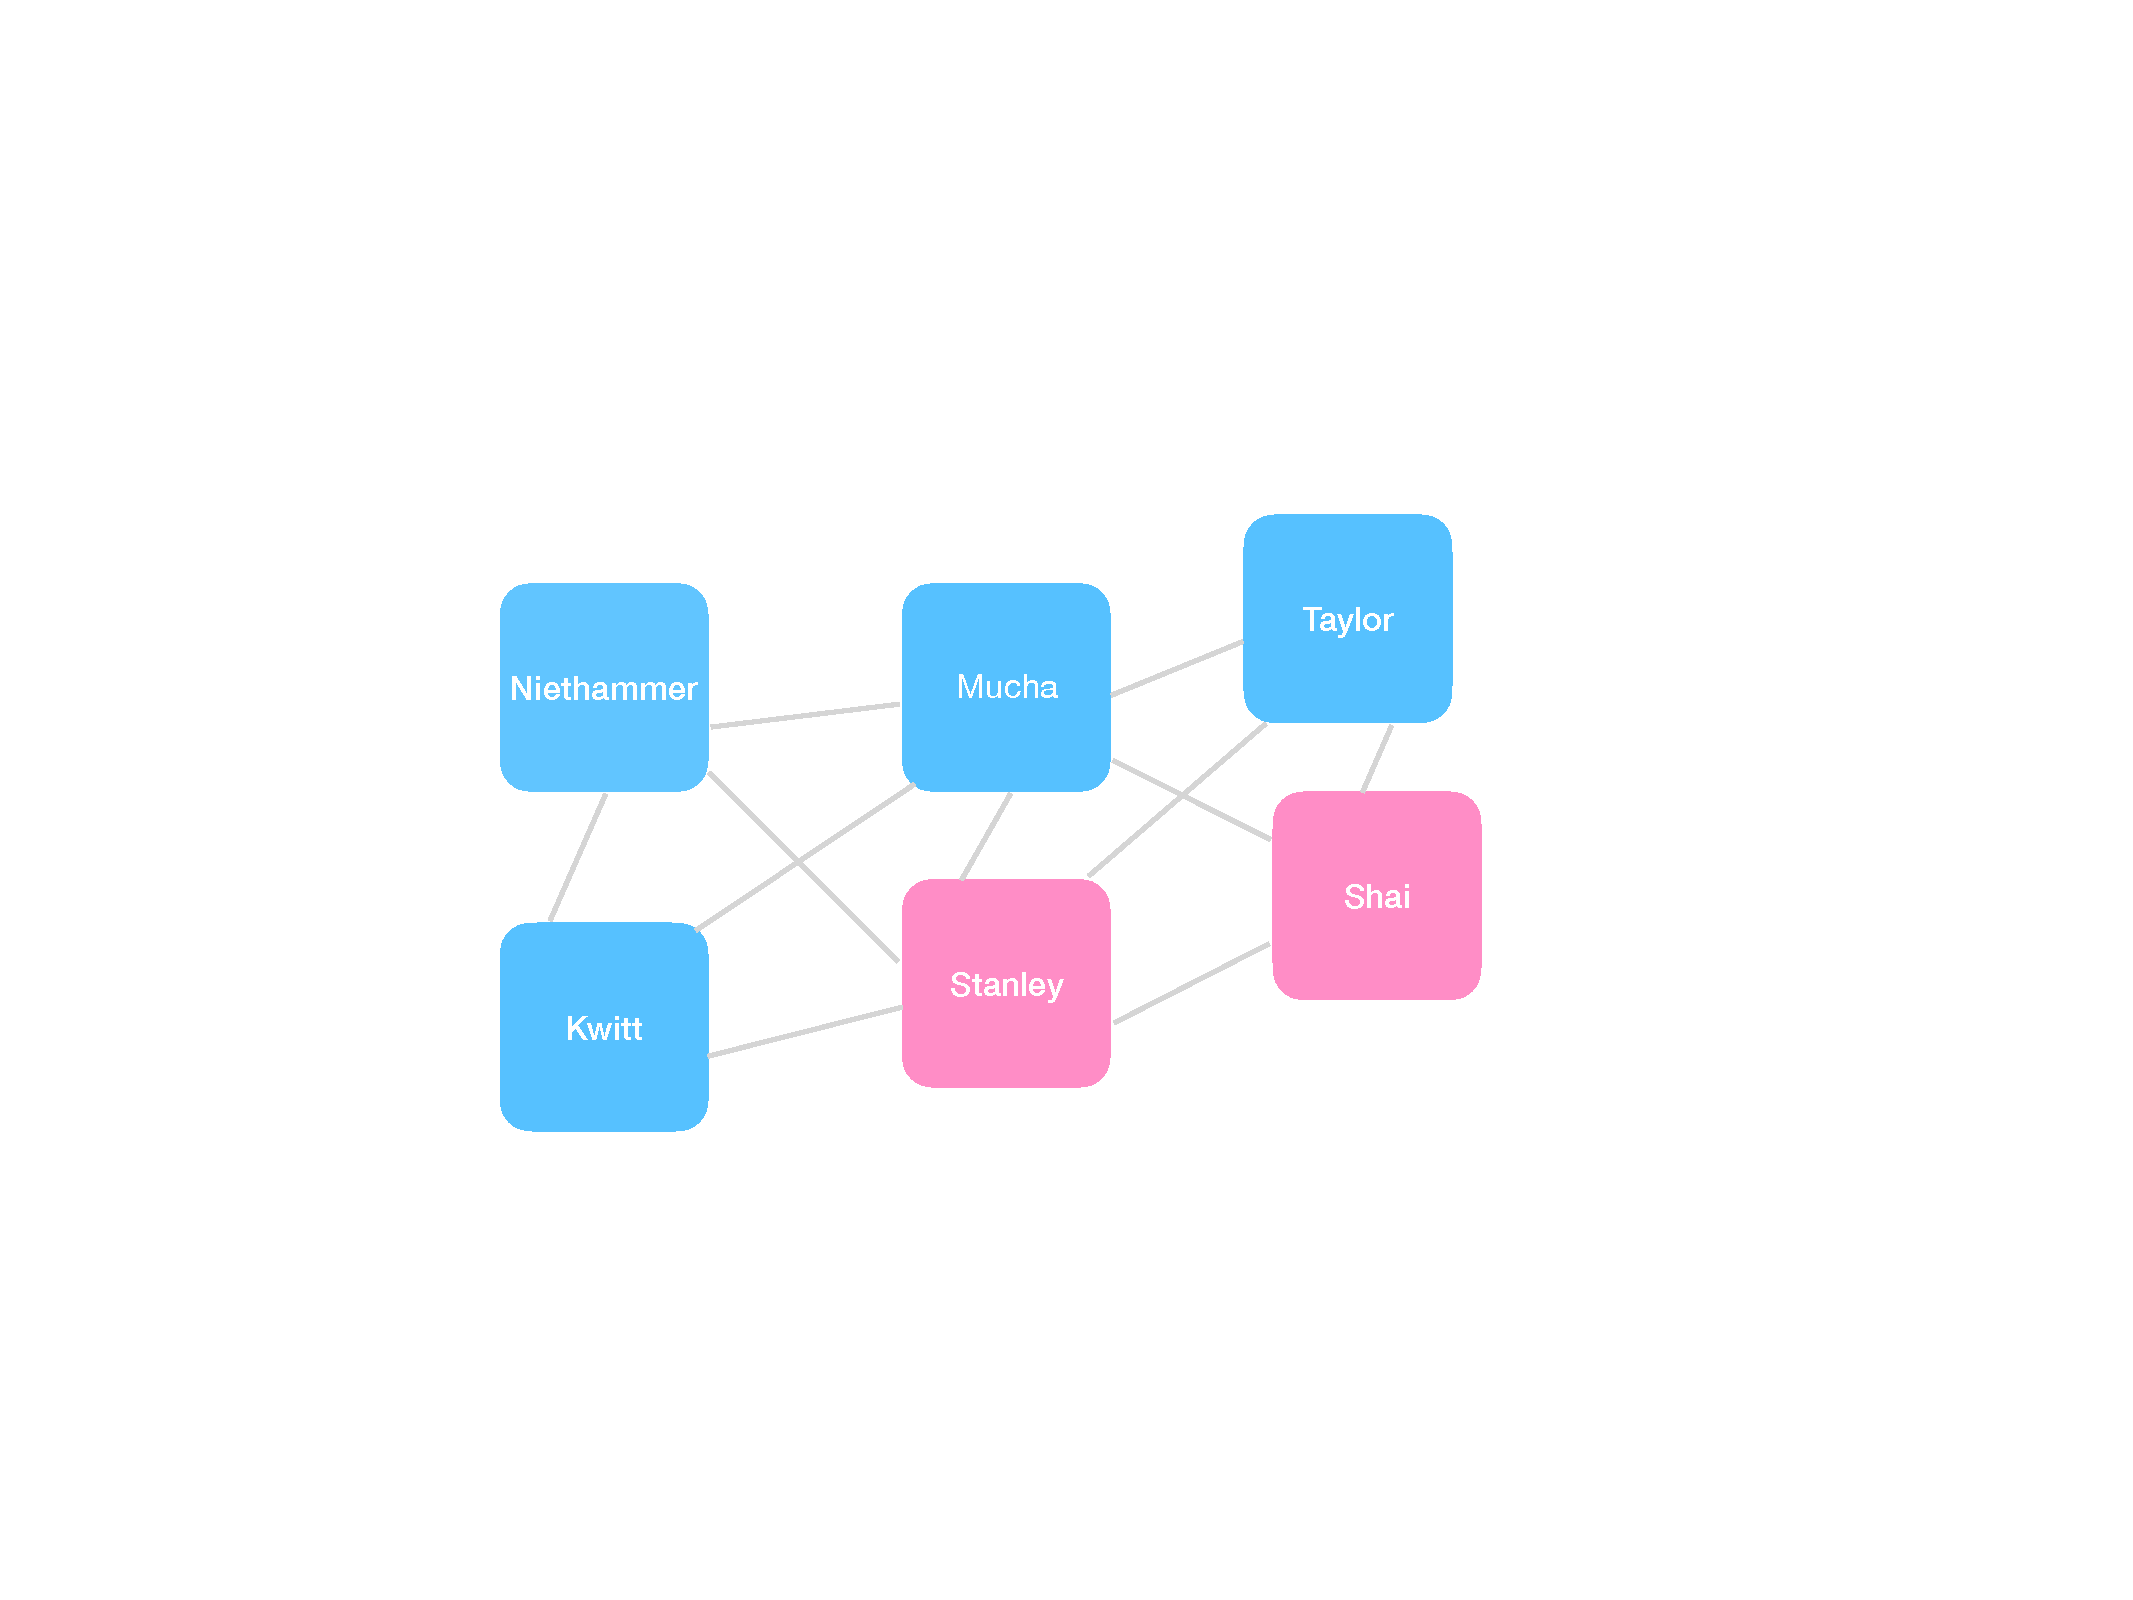
\includegraphics[scale=0.5]{CoAuthor}
\caption{{\bf A simple network example (coauthorship).} A co-authorship network with an edge between a pair of people if they have written a paper together.}
\label{fig:social}
\end{center}
\end{figure}

Such a network with edges simply representing whether or not a pair of nodes interact scientifically is an example of an \emph{undirected, unweighted} network. Among undirected networks, edges can also be weighted, which quantifies pairwise similarity between a node pair. For a set of $N$ nodes, we define the $N \times N$ network adjacency matrix, ${\bf A}=\{a_{ij}\}$. For a pair of nodes $i$ and $j$, its corresponding adjacency matrix entry $a_{ij}$ is defined as follows,

\[ \begin{cases} 
     a_{ij}=1 & \text{\emph{if node $i$ and node $j$ are connected}} \\
      a_{ij}=0 & \text{\emph{otherwise}}.
         \end{cases}
\]

In the \emph{weighted} case of undirected networks, edge weights are some real number and are frequently quantities such as correlation or pairwise similarity. A simple extension of ${\bf A}$ to an undirected, weighted network where $w$ is the edge weight between nodes $i$ and $j$, computes the adjacency matrix entry $a_{ij}$ as, 

\[ \begin{cases} 
     a_{ij}=w & \text{\emph{if node $i$ and node $j$ are connected} with weight $w$} \\
      a_{ij}=0 & \text{\emph{otherwise}}.
         \end{cases}
\]

Alternatively, the assumption of a symmetric relationship between a pair of nodes that node $i$ connects to node $j$ and node $j$ connects to node $i$  may be unrealistic. For example, on twitter, user $i$ can follow user $j$, but user $j$ does not necessarily need to follow user $i$. This type of network is known as a \emph{directed} network. While directed are frequently discussed in the network science literature, we will not introduce them here because they are not involved in any work in this thesis. 

\subsection{Network Summary Statistics}

\indent Given a network, there are fundamental tasks of interest that allow for a more clear interpretation and understanding of the data. Some of these objectives include, ranking the node by their importance or \emph{centrality} in the network, clustering nodes, and predicting the existence of a link between a node pair. Toy networks, such as the one presented in Figure \ref{fig:social} or in a textbook often look deceptively clean and well-structured. In reality, most network data is large, messy, and often referred to as a hairball. This term alludes to the difficulty of immediately discerning structure or interpreting meaning from the network due to the large amount of presented information. An example of a typical hairball is shown in Figure \ref{fig:Hairball}. Here, there are many nodes and edges that from immediate inspection, it may seem like the relational patterns are too difficult to untangle and interpret.

\begin{figure}
\begin{center}
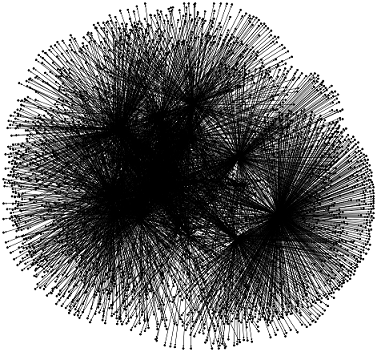
\includegraphics[scale=0.4]{Hairball}
\caption{{\bf Hairball network.} Networks are often noisy data structures and lack an immediate straight forward structural interpretation. \emph{Image from \url{https://cs.umd.edu}.}}
\label{fig:Hairball}
\end{center}
\end{figure}

\subsubsection{Example: A network representation of single cell data and simple summary statistics}

\indent An initially overwhelming network structure can be mediated by tools to break down, quantify, and characterize structural patterns. In this section, we will describe a few of the essential summary statistics and analyses that can be performed and will be seen throughout this thesis.

\indent To illustrate these quantities in an applied context, we will compute them on an example network shown in Figure \ref{fig:Cytometry}. This network is constructed from a single cell mass cytometry dataset, which was originally described in Ref. \cite{wong2015} and released publicly and processed using the Cytofkit R package \cite{cytofkit}. Each node represents a single cell and is represented with 52 features for a mass cytometry analysis. Briefly, mass cytometry is a technique to simultaneously measure multiple immunological features in a cell or tissue \cite{cytof}. From this data matrix, we created a network by selecting 500 cells and building a $k$-nearest neighbor network with $k=5$. This means that for a node $i$, we found its $5$ nearest neighbors according to Euclidean distance, and connected them all to node $i$. 

\begin{figure}
\begin{center}
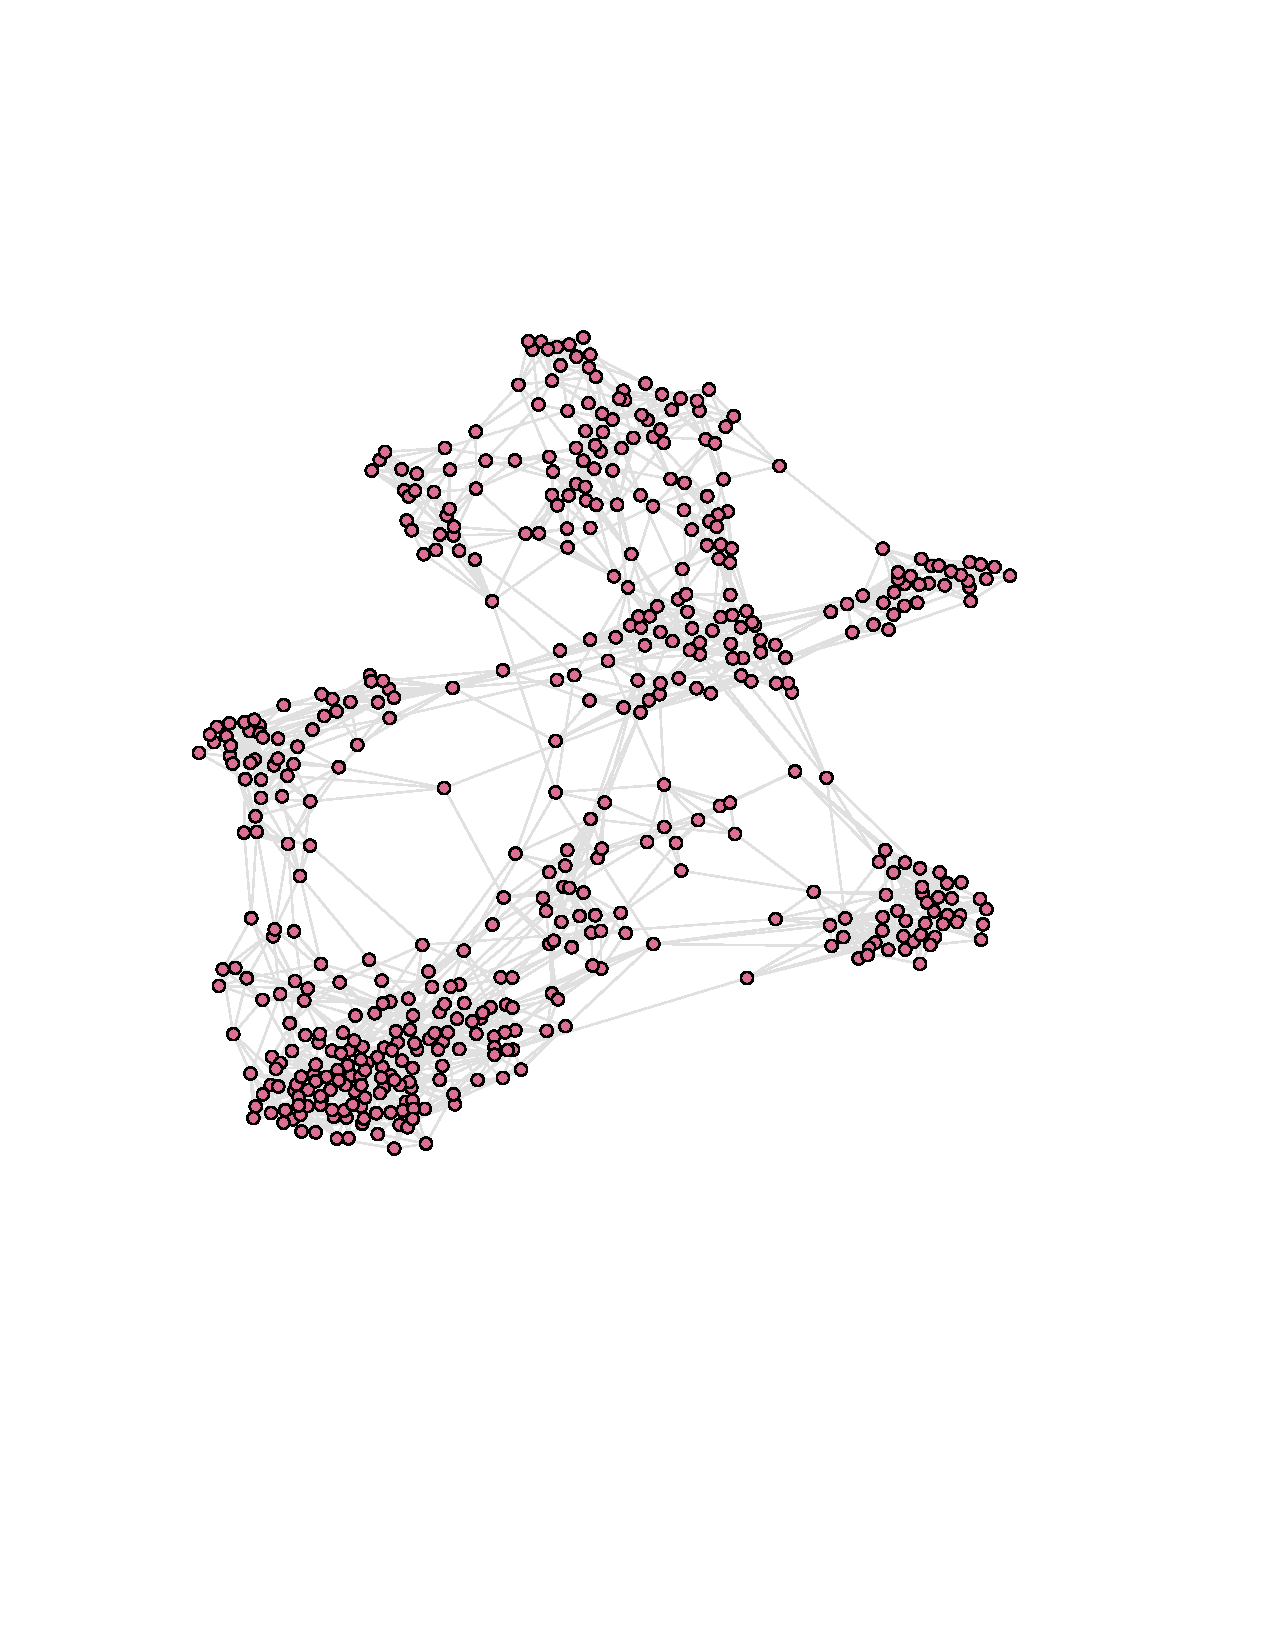
\includegraphics[scale=0.5]{CytometryNet}
\caption{{\bf Network of single cells.} We constructed a network from mass cytometry profiling among 500 cells in single cell dataset. Each cell has 52 measured immune features. In this network, each node is a single cell and is connected to its 5 nearest neighbors.}
\label{fig:Cytometry}
\end{center}
\end{figure}

\subsubsection{Degree Distribution}

Here, we will define a variety of summary statistics and quantities that can be computed on a network that give insight into the network's structure. The first most basic summary statistic is known as \emph{degree}.  Given the adjacency matrix for an undirected network, ${\bf A}$, the degree of node $i$, $\text{degree}(i)$ is computed as,

\begin{equation}
\text{degree}(i)=\sum_{j}a_{ij}
\end{equation}

\begin{figure}
\begin{center}
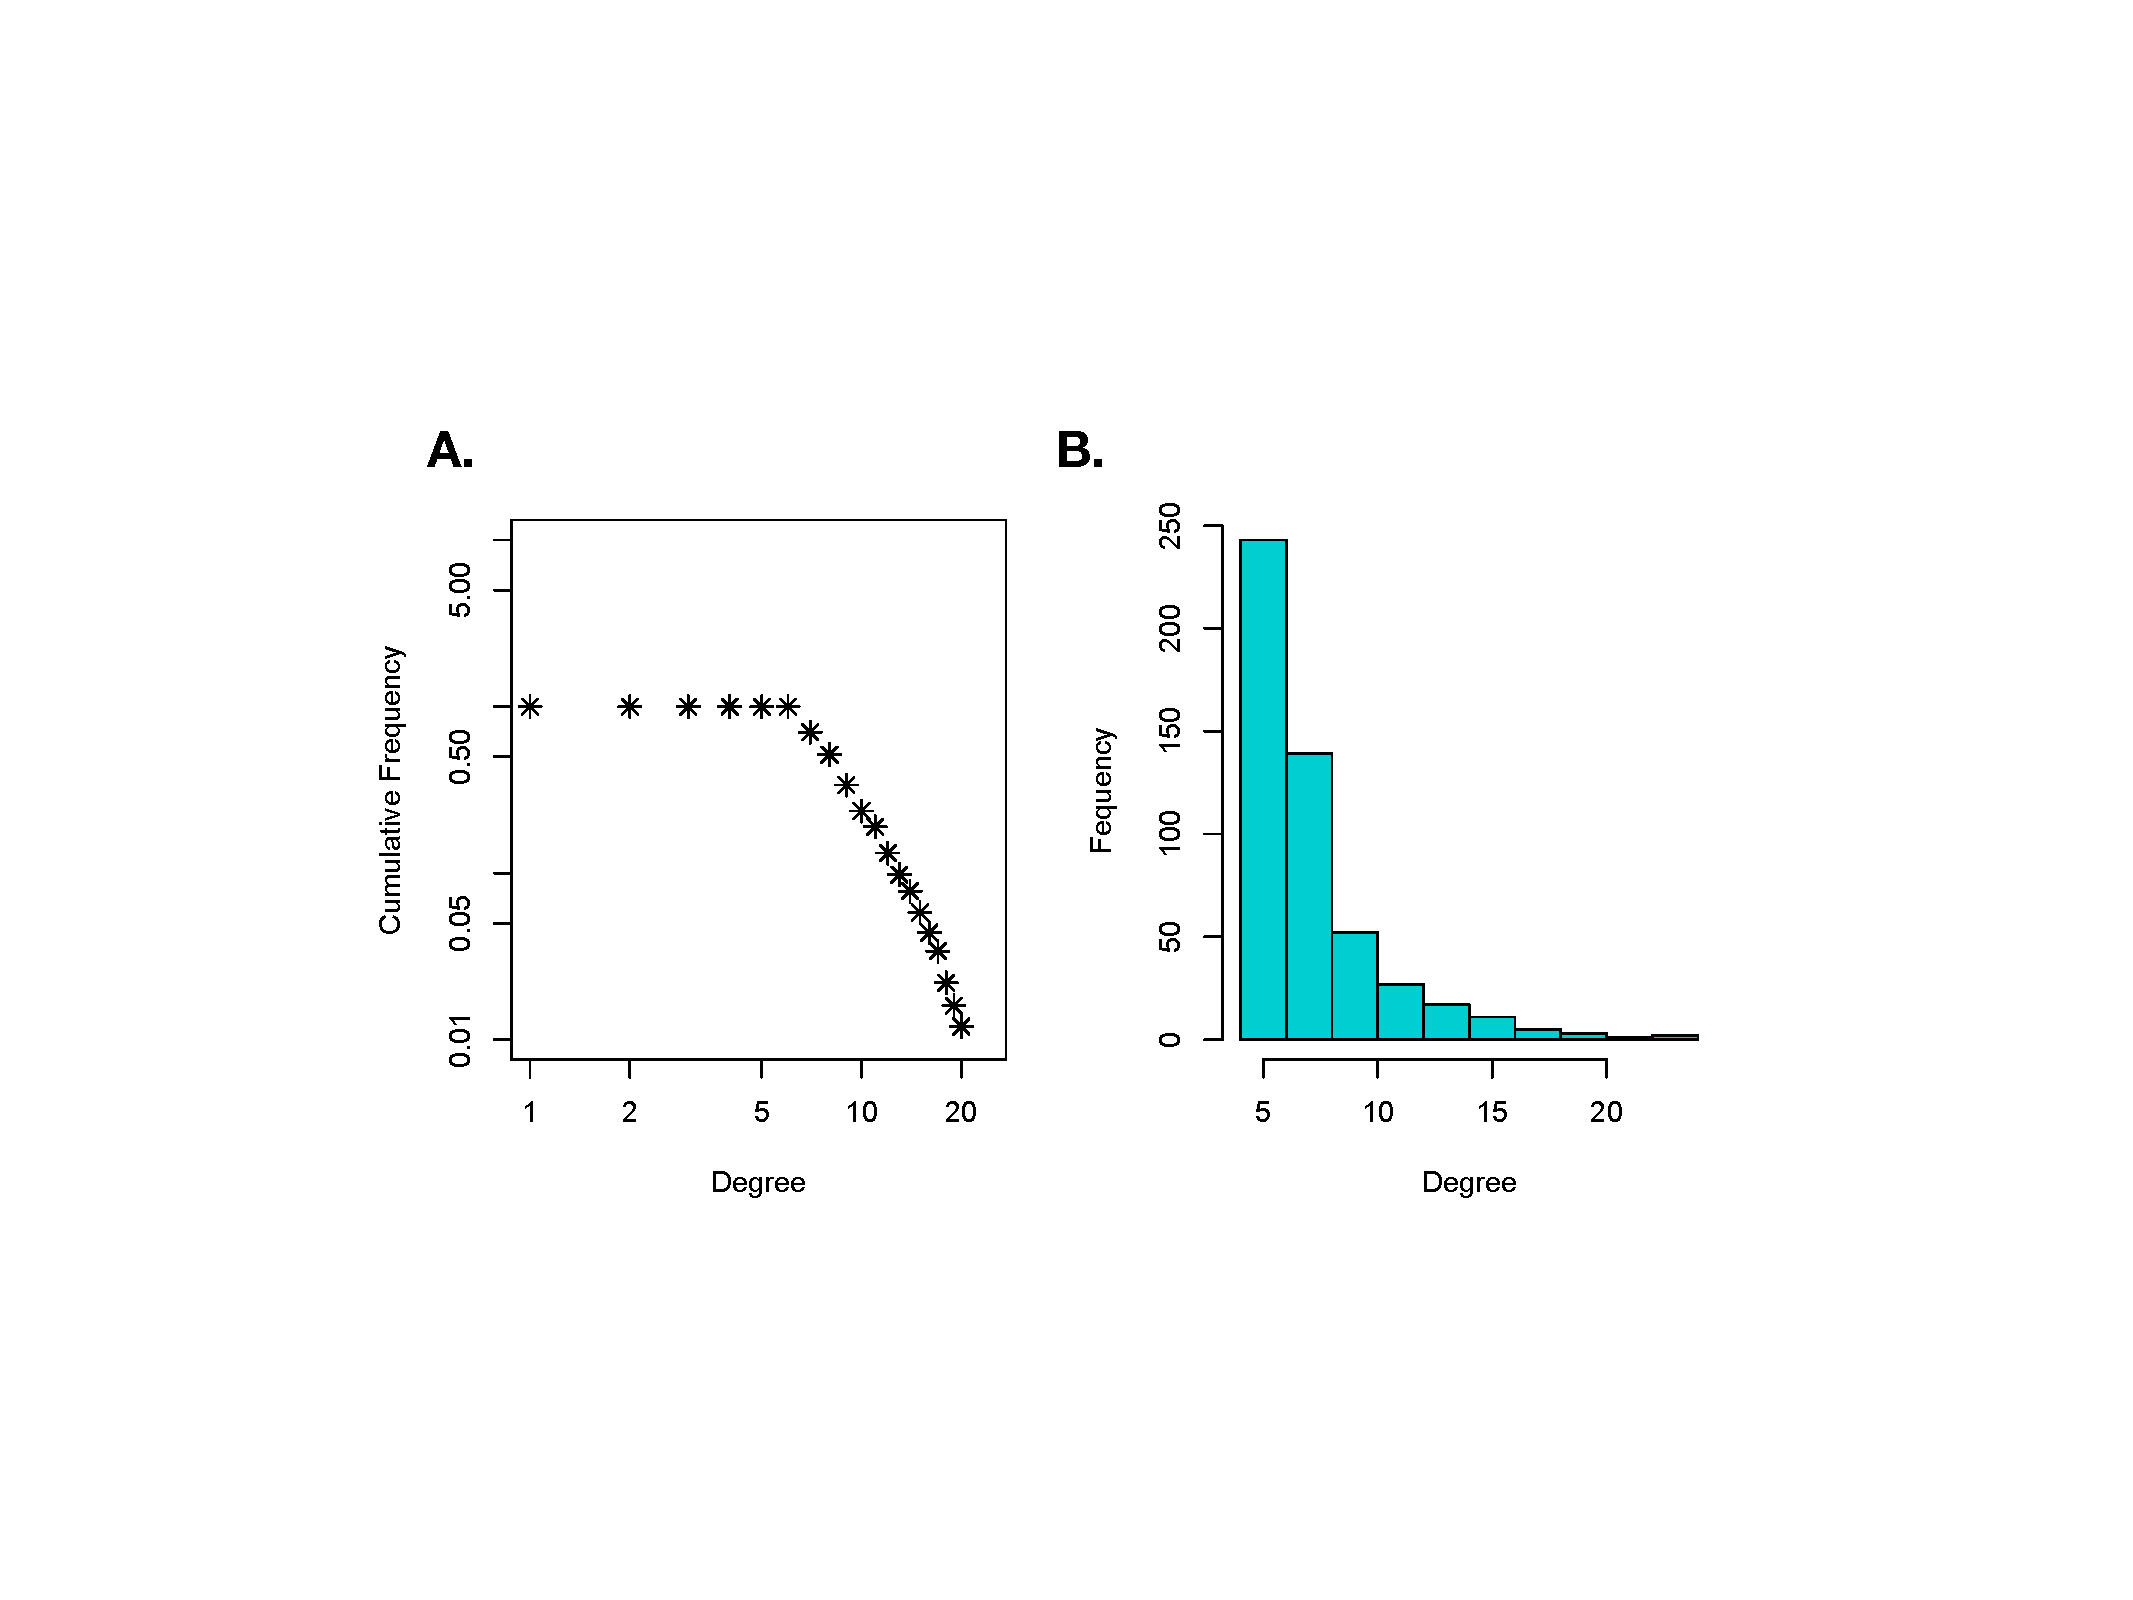
\includegraphics[scale=0.5]{DegDist}
\caption{{\bf Degree distribution for the single cell network.} We visualize the degree distribution in the single cell network presented in Figure \ref{fig:Cytometry}. {\bf A.} We compute a cumulative distribution plot for degree. {\bf B.} Node degrees can also be visualized with a simple histogram.}
\label{fig:DegDist}
\end{center}
\end{figure}

In the case of an undirected, unweighted network, the degree of node $i$ counts its number of neighbors, while in the undirected, weighted context, degree encodes the total edge weight incident to node $i$. Collectively examining the distribution of degrees for a network is known as the \emph{degree distribution}. Understanding the degree distribution provides insight into the network type and structural organization.  We visualize degree distribution in Figure \ref{fig:DegDist} using a cumulative distribution plot (A.) and a simple histogram (B.). Since this network was constructed with a $5$-nearest neighbor rule, we see this reflected in the degree distribution, with all nodes having degree 5 or more. A few nodes have significantly higher degree ($> 10$) and represent single cells who is a nearest neighbor to many of the other cells in the original 52 dimensional space. A node's degree is often highly related to its importance in the network, which provides a nice transition to the next set of summary statistics, network centrality measures.

\subsubsection{Centrality}
\indent To compute the importance of a node in the network it is common to compute a centrality score. There are many definitions of centrality, and we will only present a small subsets of these definitions here. We all benefit from the idea of high centrality nodes, when we do a Google search and have a relevant page of returned search results. In this section, we introduce, degree centrality, betweenness centrality, and eigenvector centrality. Given that each of these measures is computed differently, each is intended to capture a different structural aspect of the network. 

 \begin{figure}[h!]
\begin{center}
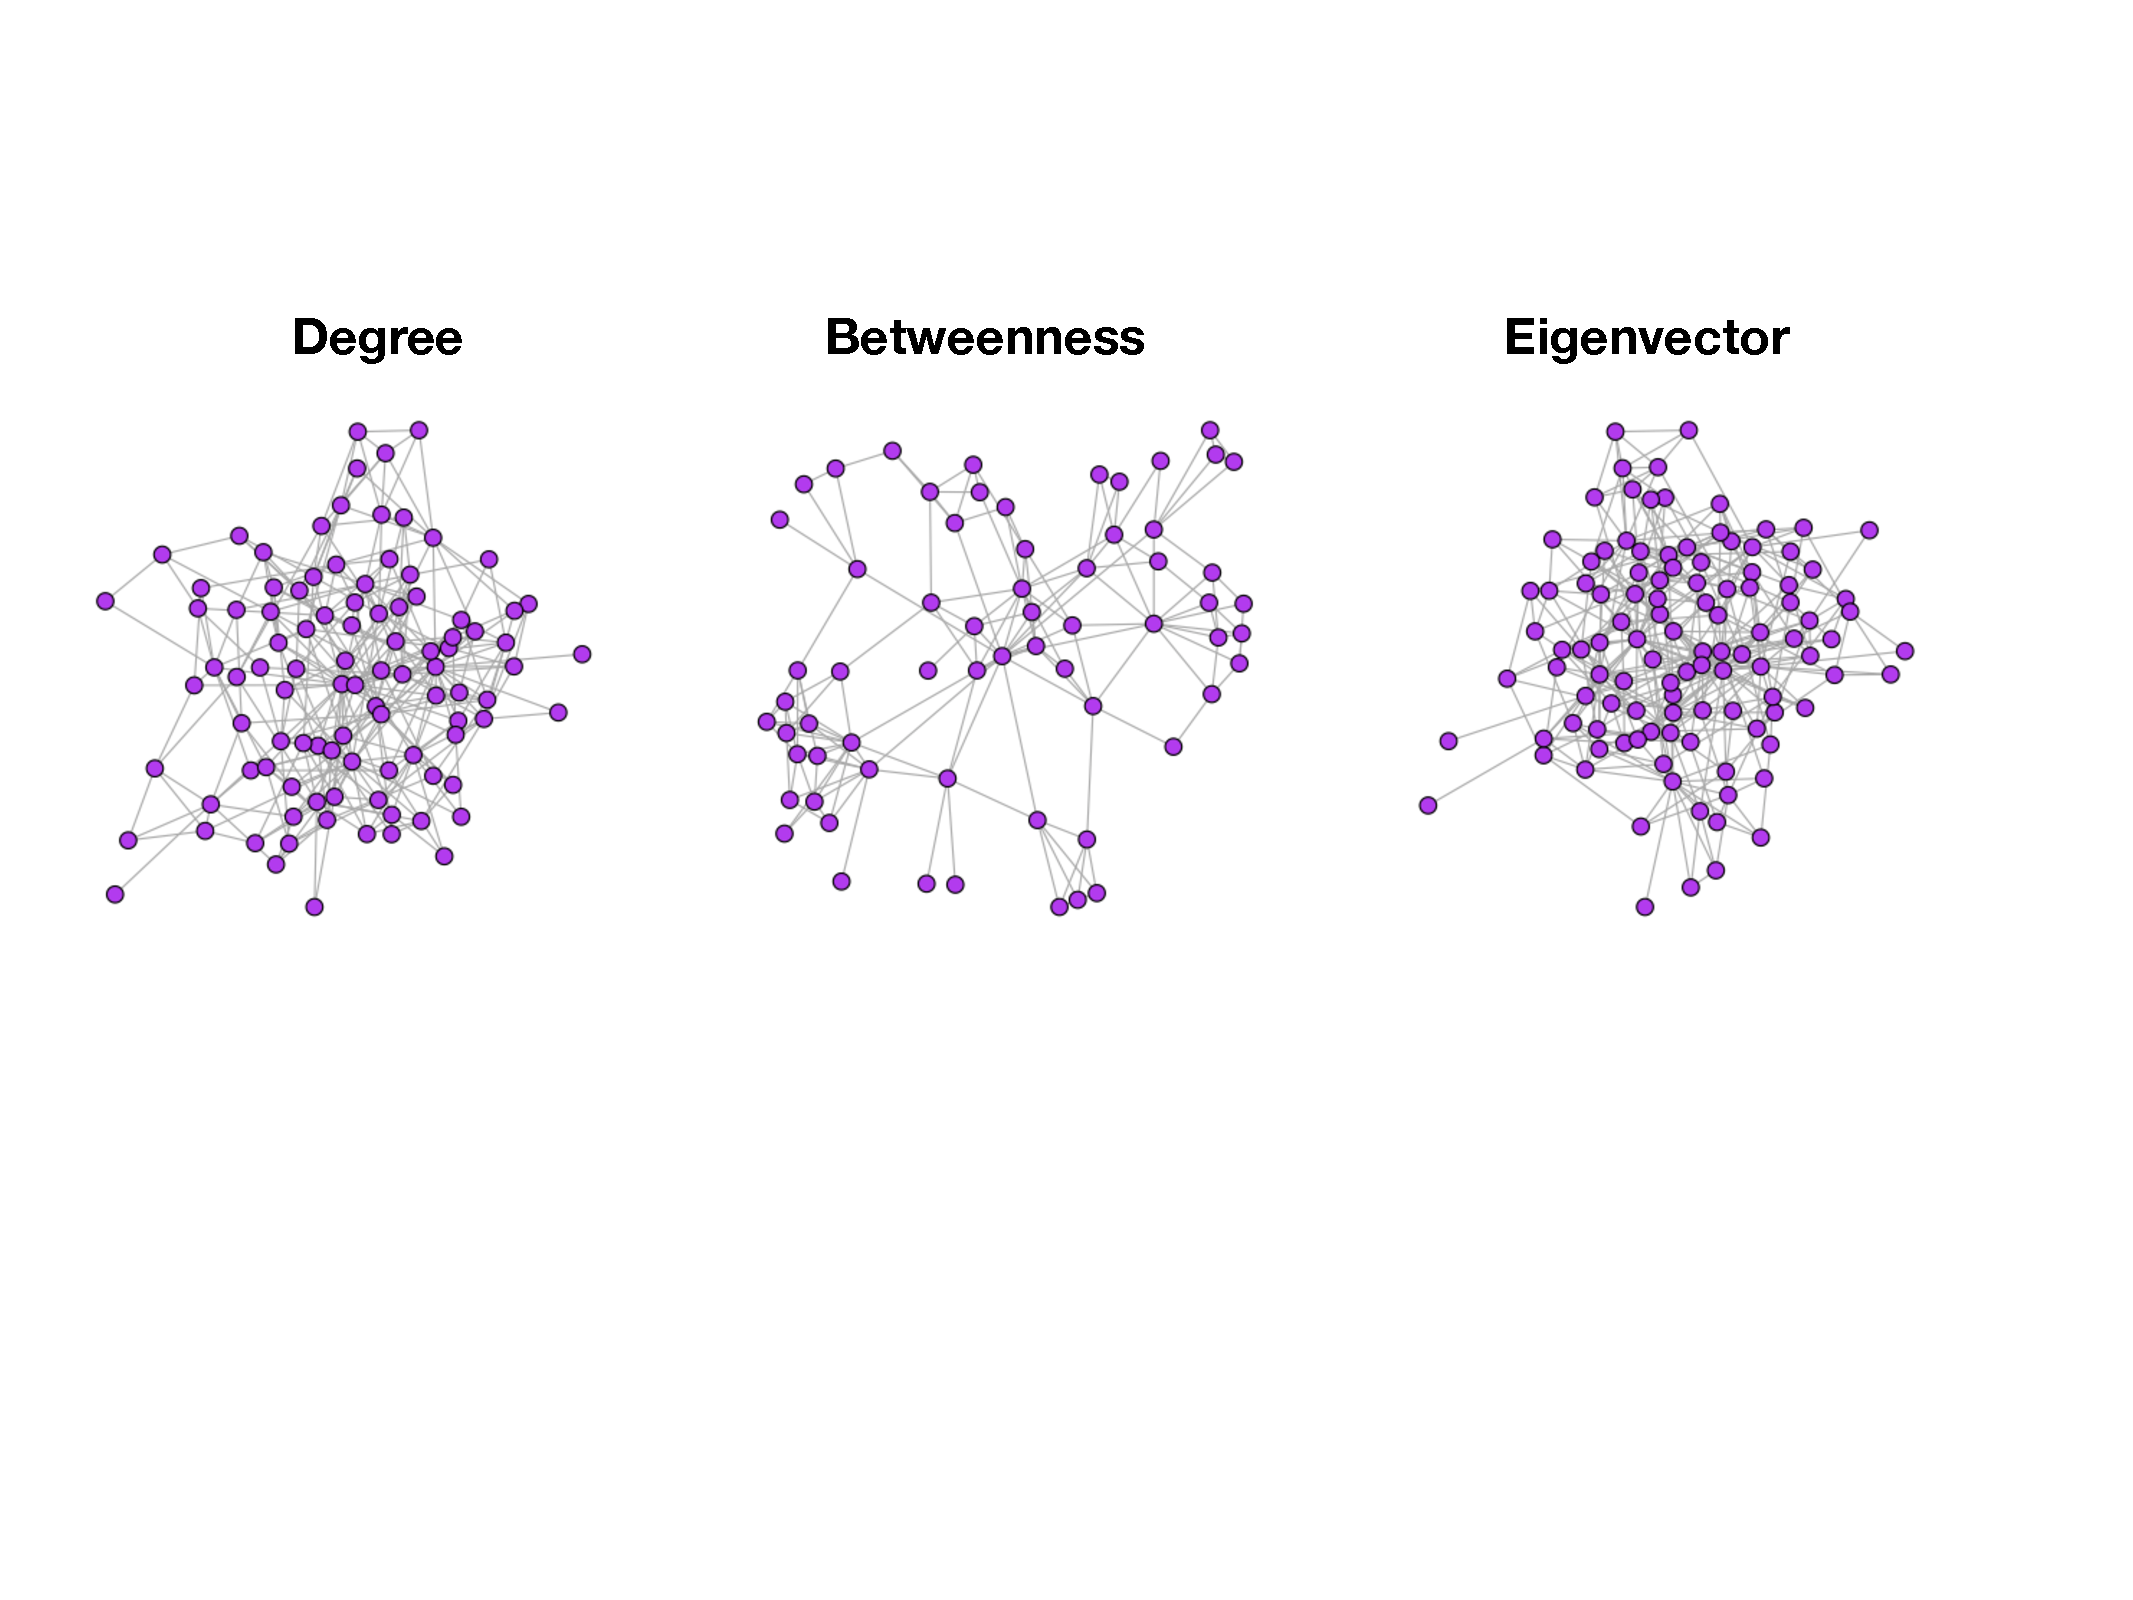
\includegraphics[scale=0.4]{Centrality}
\caption{{\bf Centralities on the single cell network.} The second order ego network for the highest centrality nodes in the single cell network according to degree, betweenness, and eigenvector in the left, center, and right plots, respectively. These plots are meant to emphasize how each of these centrality measures prioritizes different kind of stucture.}
\label{fig:Centrality}
\end{center}
\end{figure}

{\bf Degree centrality}\\
Degree centrality is the most simple centrality measure because it is just simply a node's degree. This means that under this measure, the most important nodes in the network are nodes with high degree. This centrality is attractive because it is easy to compute, having complexity in a sparse network of $O(E)$ (where $E$ is the number of edges). We define degree centrality of node $i$, $\mathcal{D}(i)$ as,

\begin{equation}
\mathcal{D}(i)=\sum_{j}a_{ij}
\end{equation}

{\bf Betweenness centrality}\\
Betweenness centrality quantifies node importance, based on how many shortest paths go through a node. So, if a node appears on many of the shortest paths between node pairs, then it is considered to be an important node. We define betweenness centrality for a node $i$, $\mathcal{B}(i)$ as,

\begin{equation}
\mathcal{B}(i)=\sum_{i\ne j\ne t} \frac{\sigma_{jt}(i)}{\sigma_{jt}},
\end{equation}

where $\sigma_{jt}$ is the total number of shortest paths between a pair of nodes, $j$ and $t$ that pass through $i$. \\

{\bf Eigenvector centrality}\\
The idea behind eigenvector centrality is that a node should be prioritized not only based on its degree, but the degree of its neighboring nodes. That is, a node connected to other `important' or high degree nodes should be ranked higher than one connected to many low degree nodes \footnote{If you want to compliment a friend, it is nicer to say that they have high eigenvector centrality than high degree centrality.}. The eigenvector centrality for node $i$, can be computed using the spectra of the adjacency matrix, ${\boldsymbol A}$. In particular, the vector of centralities, ${\bf x}$ is the one satisfying the eigenvector equation,

\begin{equation}
{\bf A}{\bf x}=\lambda{\bf x}.
\end{equation}

Because centralities are non-zero, the solution must be an eigenvector with all positive entries. Since multiple eigenvalues ($\lambda$) correspond to non-zero eigenvectors, the eigenvector corresponding to the largest eigenvector is used and the centrality scores for each node reflect its relative importance in comparison to the rest of the nodes. Moreover, the $i$-th entry of ${\bf x}$ gives the eigenvector centrality for node $i$. \\

\indent We visualized the results of each of these three presented centralities on the single cell network data in Figure \ref{fig:Centrality}. Under each of the centrality measures, we selected the the highest-ranked centrality node and focused in its local ego network. This is shown for degree, betweenness, and eigenvector centralities in the left, middle, and right panels respectively. In particular from these high centrality nodes, we visualized their corresponding order 2 ego networks.  An ego network for node $i$ is simply the subgraph of all nodes within two hops of node $i$. This visualization gives a sense of what kinds of connectivity patterns each centrality measure favors. For example, we see that degree and eigenvector centrality have similar ego networks, as they are capturing nodes with a lot of connections. However, the ego network of the high betweenness centrality node is serving as more as a bridge between densely connected parts of the network. 

\section{Introduction to community detection}
While centrality measures allow for the prioritization of individual nodes in the network, it is also useful to look at sets of similar nodes in terms of how they are situated in the network. Each of these sets of similar nodes is known as a \emph{community}. A community in a network is broadly defined as a set of nodes of who share something in common in terms of their connectivity patterns in the network. One can think of a community as a clustering problem on networks, where the objective is to define sets of nodes that maximize the within-community node similarity. The most basic type of community to understand is a network with assortative community structure. In this case, nodes are tightly connected to each other but more sparsely connected to the rest of the network. An example of a network with assortative community structure is shown in Figure \ref{fig:Assort}. Communities in the network are outlined with pink dotted lines.

 \begin{figure}
\begin{center}
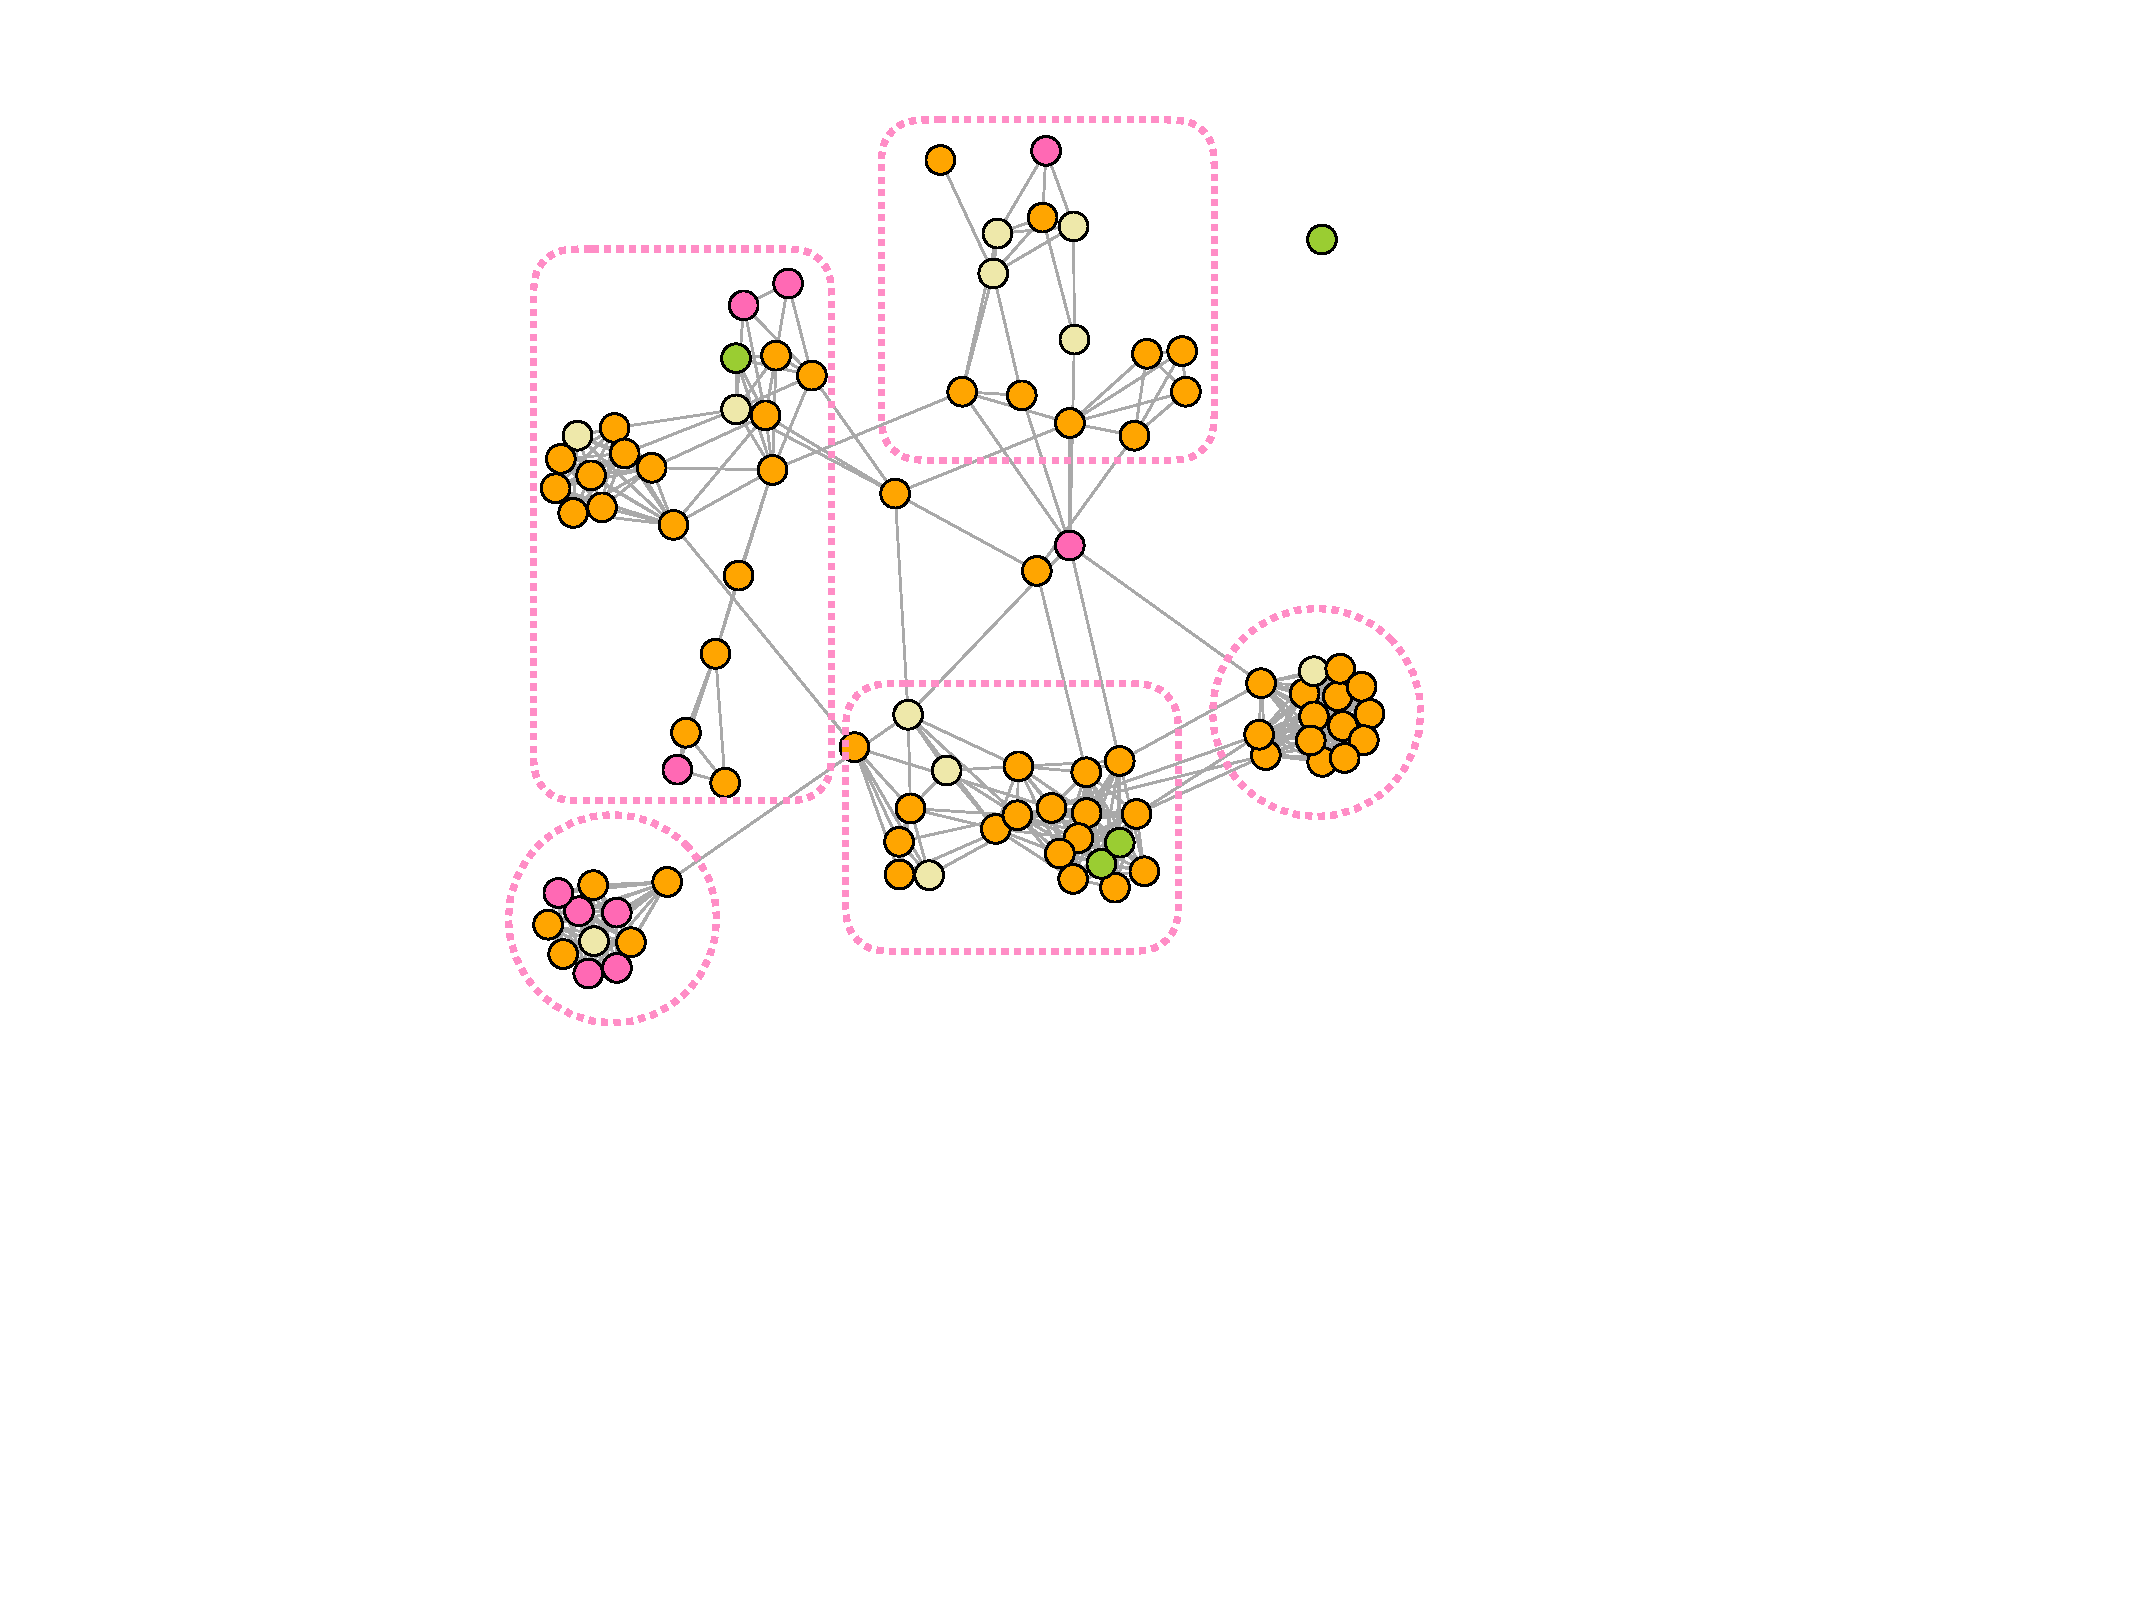
\includegraphics[scale=0.4]{AssortativeNet}
\caption{{\bf Assortative Community Structure.} This network is an example of assortative community structure, where nodes are tightly connected to each other and more sparsely connected to the rest of the network. Each community is outlined with a pink dotted line.}
\label{fig:Assort}
\end{center}
\end{figure}

Alternatively, networks can have a disassortative structure where the between community edge density exceeds the within-community density. Finally, a core periphery structure can arise when there is a central core in the network that connects to the rest of the network and a set of peripheral nodes that connect to the core, but not to each other.  Similar to how the shape or distribution of a set of points in high dimensional space informs the ideal clustering algorithm to use, aspects of these diverse types of community structure often prescribe which algorithm to use. For a great explanation about common types of community structure in network data which patterns have been observed in the human brain, please refer to Betzel \emph{et al.} \cite{betzel}.  

In this section, we have only briefly introduced the history and intuition behind community detection. Since it is a well-developed domain of network science, the interested reader can refer to one of the comprehensive review articles \cite{fortu1,fortu2,shaicase,muchacommunity}

\section{Community detection methods}
When performing community detection on a network, the objective is to segment nodes into one of $K$ communities. This $K$ can be known apriori or estimated through some kind of model selection criterion or through quality function computations. There are many optimization approaches that can be used to approach network community detection. In this section, we will introduce the current state-of-the-art approaches characterized as quality function maximization, deep learning, higher order clustering, and probabilistic methods. These methods are discussed based on their ability to handle networks of non-trivial size with diverse structures. We particularly elaborate on the stochastic block model and modularity maximization, as those are the the approaches considered throughout the novel work in this thesis.  

\subsection{Notation for Community Detection}
We first define some common notation for community detection. For a network with $N$ nodes, we use a community detection algorithm to separate these nodes into $K$ communities. To encode the node-to-community assignments, we use the length $N$ vector, ${\bf z}$, where $z_{i}$ gives the community assignment for node $i$. For some applications, we also specify the $N \times K$ matrix, ${\bf Z}$, which is a binary indicator matrix, where $z_{ik}$ indicated whether node $i$ is assigned to community $k$. These two pieces of notation will be used across each of the described algorithms. 

\subsection{Quality function maximization with modularity}
\indent In quality function optimization approaches one first specifies an objective function in terms of a partition of the nodes. The most common quality function for this task is known as modularity \cite{newman2006modularity}. Modularity first defines a null model for community structure where edges are places between groups randomly. With this as the starting point, the partition that optimizes modularity is the one that is maximally different from this null model. In particular, this null model is a random graph model, known as the configuration model \cite{benderCanfield}. To generate an $N$-node network from the configuration model, one first specifies a fixed degree sequence, $D=\{k_{i},k_{2},\dots,k_{N}\}$. From this sequence, nodes are connected with $k_{i}$ stubs that will ultimately be connected together. Finally, the graph is constructed by randomly choosing pairs of the created stubs and joining them. Based on how this network was generated, it is easy to specify the probability that an edge exists between a pair of nodes, $i$ and $j$, or $P(a_{ij}=1)$.

\begin{equation}
P(a_{ij}=1)=\frac{k_{i}k_{j}}{2M}.
\end{equation}

Here, $k_{i}$ and $k_{j}$ represent the degree for nodes $i$ and $j$, respectively, and $M$ is the total number of edges in the network. 

\indent Modularity was introduced in 2004 by Newman and Girvan \cite{newmangirvan}. We define the modularity quality function, $Q$ as,

\begin{equation}
Q=\frac{1}{2M}\sum_{i,j}\left[a_{ij}-\gamma \frac{k_{i}k_{j}}{2M}\right]\delta(z_{i},z_{j})
\end{equation} 

Here, $\gamma$ is a resolution parameter \cite{resParam} that controls the scale of community size. Large values of $\gamma$ favor more small communities while smaller values enforce fewer large communities. 

\indent In order to determine ${\bf z}$, the most computationally efficient approach is known as the Louvain algorithm \cite{blondel}. The Louvain algorithm is an agglomerative heuristic, which initially starts with each node in its own community and in the first pass merges pairs of nodes if their merge leads to an increase in modularity. Each group of nodes assembled after this first pass becomes a new node in the network and a new weighted network is created between the set of new nodes. The weight on the edges of the new network are the number of edges from the original network that go between the sets of merged nodes. This process is continued iteratively until the modularity no longer increases. The reason that this approach is so computationally tractable is because the gain in modularity, $\Delta Q$ of merging two groups of nodes can be explicitly computed in closed form.

\indent Modularity has shown to be effective in applications from neuroscience \cite{hierarchicalmod} to image segmentation \cite{browet}. It has also shown to be effective in clustering high dimensional data that has been used to create a network. In Figure \ref{fig:clustering}, we used tSNE \cite{TwoD} to project the 52-dimensional single cell data into 2 dimensions. Points are colored by their cluster assignment according to $k$-means. We first performed $k$-means on the original 51 dimensional data (left) and Louvain community detection on the 5 nearest neighbor network representation (right). One benefit of the Louvain algorithm is that it does not require specifying the number of clusters. Moreover, in this example, the Louvain algorithm maximized modularity by partitioning the network into 10 clusters. To compare the results under the same number of clusters, we also clustered the original data into 10 clusters. From these two partitions, we observe that creating a network representation of the data before clustering assists in identifying the smaller, less prominent clusters.


 \begin{figure}
\begin{center}
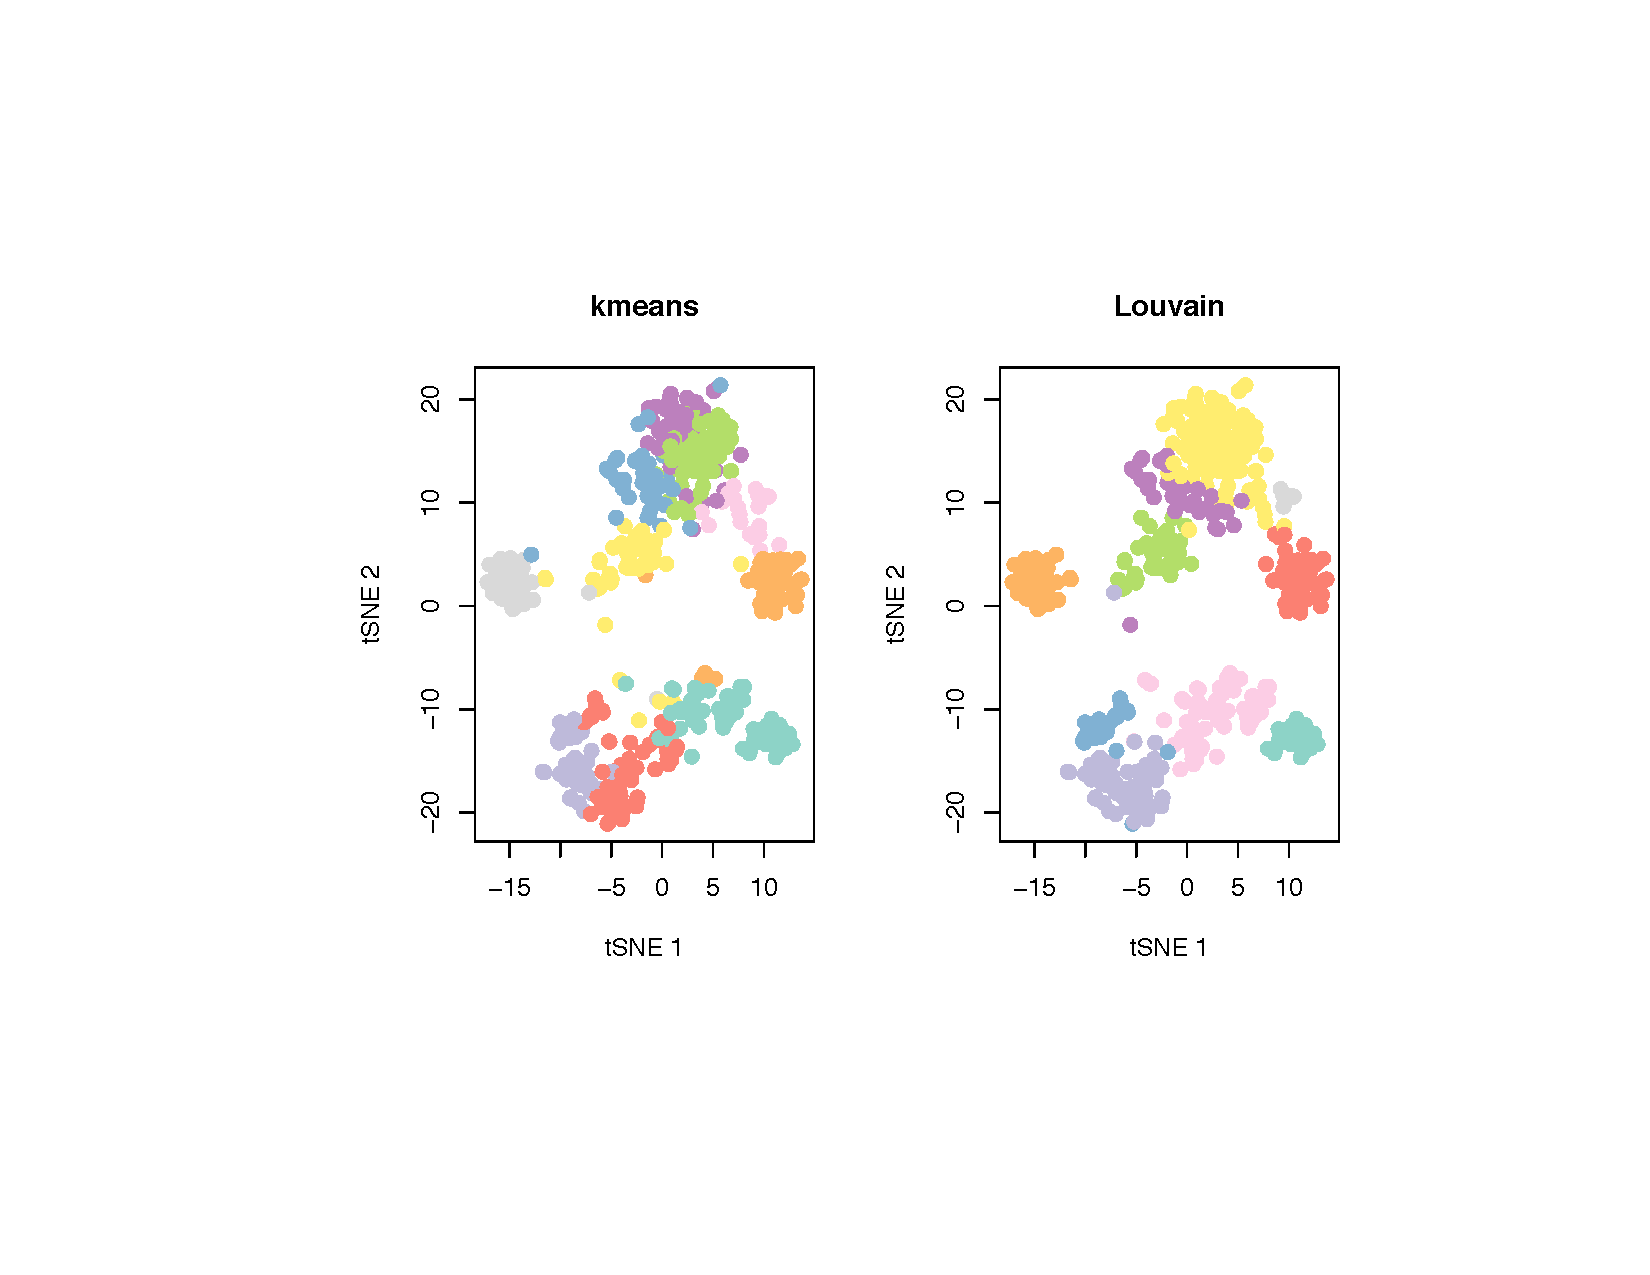
\includegraphics[scale=0.5]{clustering}
\caption{{\bf A comparison of $k$-means and the Louvain algorithm on the single cell network.} A comparison of the results of clustering results on the the single cell dataset through $k$-means on the original 52-dimensional data (left) and by the Louvain algorithm on the nearest neighbor network (right). Each of the single cells (or nodes in the nearest neighbor network) is visualized by a 2-dimensional projection frin tSNE. Points are colored by their cluster membership under $k$-means on the original data (left) and Louvain community detection (right). Applying community detection to the nearest neighbor network seems to smooth out the partition and identify some smaller clusters. }
\label{fig:clustering}
\end{center}
\end{figure}

\subsection{Identifying communities with probabilistic approaches}

\indent Probabilistic community detection methods aim to find a partition of the network through likelihood optimization. Intuitively, the goal is to study the generative process of the node edges in terms of the inferred community assignments. For example, given nodes $i$ and $j$, one may model $P(a_{ij}=1)$ as $g(z_{i},z_{j})$, where $g(\cdot)$ is some rule based on the node-to-community assignments. Two common probabilistic community detection models are the stochastic block model \cite{originalSBM} and the affiliation model \cite{affil}. The definition and description of these models and inference techniques are described in depth in this section. To facilitate working with probabilistic models, we first introduce some notation and background on inference techniques. 

\subsubsection{Probabilistic graphical models for statistical inference}
\label{pgm}
Probabilistic community detection methods are one approach to community detection that seek to model edge existence based on the inferred node-to-community assignments. In doing so, the objective is to learn the node-to-community assignments that make the structure of the observed network the most likely. This is accomplished through likelihood optimization. To fit a probabilistic network model to data, we will define some useful notation and concepts that help simplify writing down and interpreting the likelihood. 

When modeling the node-to-community assignments in a network, we often have at least two random variables and their dependency relationships to understand. First, we are interested in ${\bf z}$, the node-to-community assignments, and ${\bf A}$, the observed adjacency matrix. Probabilistic graphical models \cite{koller} enable efficient specification and manipulation of large probability distributions through semantic structures.

As a brief example, given a set of random variables, $\{A,B,C,D,E,F\}$, we seek to compute the joint distribution, $P(A,B,C,D,E,F)$. This joint distribution can be expressed with a directed acyclic graph (DAG), whose structure encodes dependencies between random variables. The DAG allows for the representation of the joint distribution in a factorized way, which is computationally useful. A DAG between the set of random variables, $\{A,B,C,D,E,F\}$ is shown in Figure \ref{fig:DAG}. Each node in the graphical model represents an random variable and a directed edge from node $i$ to node $j$ implies that node $j$ depends on node $i$. 

\begin{figure}
\begin{center}
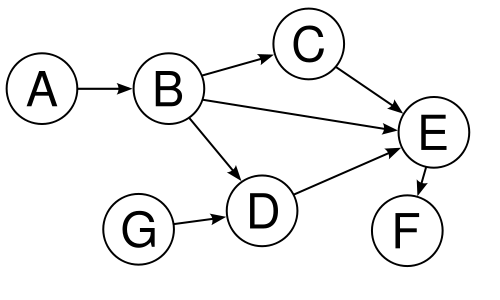
\includegraphics[scale=0.3]{DAG}
\caption{{\bf Directed Acyclic Graph.} A directed acyclic graph (DAG) is formed based on dependency between random variable and allows for a fully factorized probability distribution. Nodes represent random variables and a directed edge from node $i$ to node $j$ indicates that node $j$ depends on node $i$.}
\label{fig:DAG}
\end{center}
\end{figure}

To translate a DAG between a set of $N$ random variables, ${\bf X}=\{X_{1},X_{2},\dots,X_{N}\}$ (also in this context referred to as a Bayesian network) to its joint distribution, we rely on the chain rule for Bayesian networks \cite{koller}, which specifies that a DAG factors according to its parent/child relationships with,

\begin{equation}
P({\bf X})=\prod_{i=1:N}P(X_{i} \mid {\bf X}_{\pi_{i}}).
\end{equation}

Here, ${\bf \pi}_{i}$ denotes the set of parents for node $i$. Using this information, we can write down the joint distribution for Figure \ref{fig:DAG} as,

\begin{equation}
\begin{split}
P(A,B,C,D,E,F)&=P(A)P(B\mid A)P(C\mid B)\\
&\times P(D \mid B,G)P(E \mid D,B,C)P(F\mid E).
\end{split}
\end{equation}

This introduced idea will help in subsequent sections to expresses a model graphically, write down the model likelihood, and use the likelihood to optimize for the most appropriate model parameters. 

\subsubsection{Stochastic Block Model}
In this section, we introduce the most popular  probabilistic model for community structure, known as the Stochastic Block Model \cite{sbmorig}. This model is popular and has been studied extensively, due to its simplicity and intuitive interpretation. The crucial assumption of the stochastic block model is that nodes within a community are connected to nodes within their community and to other communities in a characteristic way. For an undirected, unweighted network with adjacency matrix ${\bf A}$, we seek to partition each of the $N$ nodes into one of $K$ communities. We denote the the node-to-community assignments as ${\bf z}$, with $z_{i}$ specifying the community assignment of node $i$. Here, ${\bf z}$ is a latent variable, with each entry taking on 1 of $K$ states, or one of $K$ community assignments. Figure \ref{fig:graphical} shows the dependency relationship between the node-to-community assignments (${\bf z}$) and the network's adjacency matrix (${\bf A}$). Here, the node-to-community assignments are treated as a latent variables because we seek to identify the ${\bf z}$ that makes the observed adjacency matrix, ${\bf A}$ the most likely. To model the objective that members within and between communities connect in characteristic ways, the model fitting procedure requires learning a set of within and between community connection probabilities. Under this approach, edges are treated as independent and identically distributed and deciding whether or node an edge exists between a pair of nodes is the learned connection probability between the communities to which each of the nodes belong.

\begin{figure}
\begin{center}
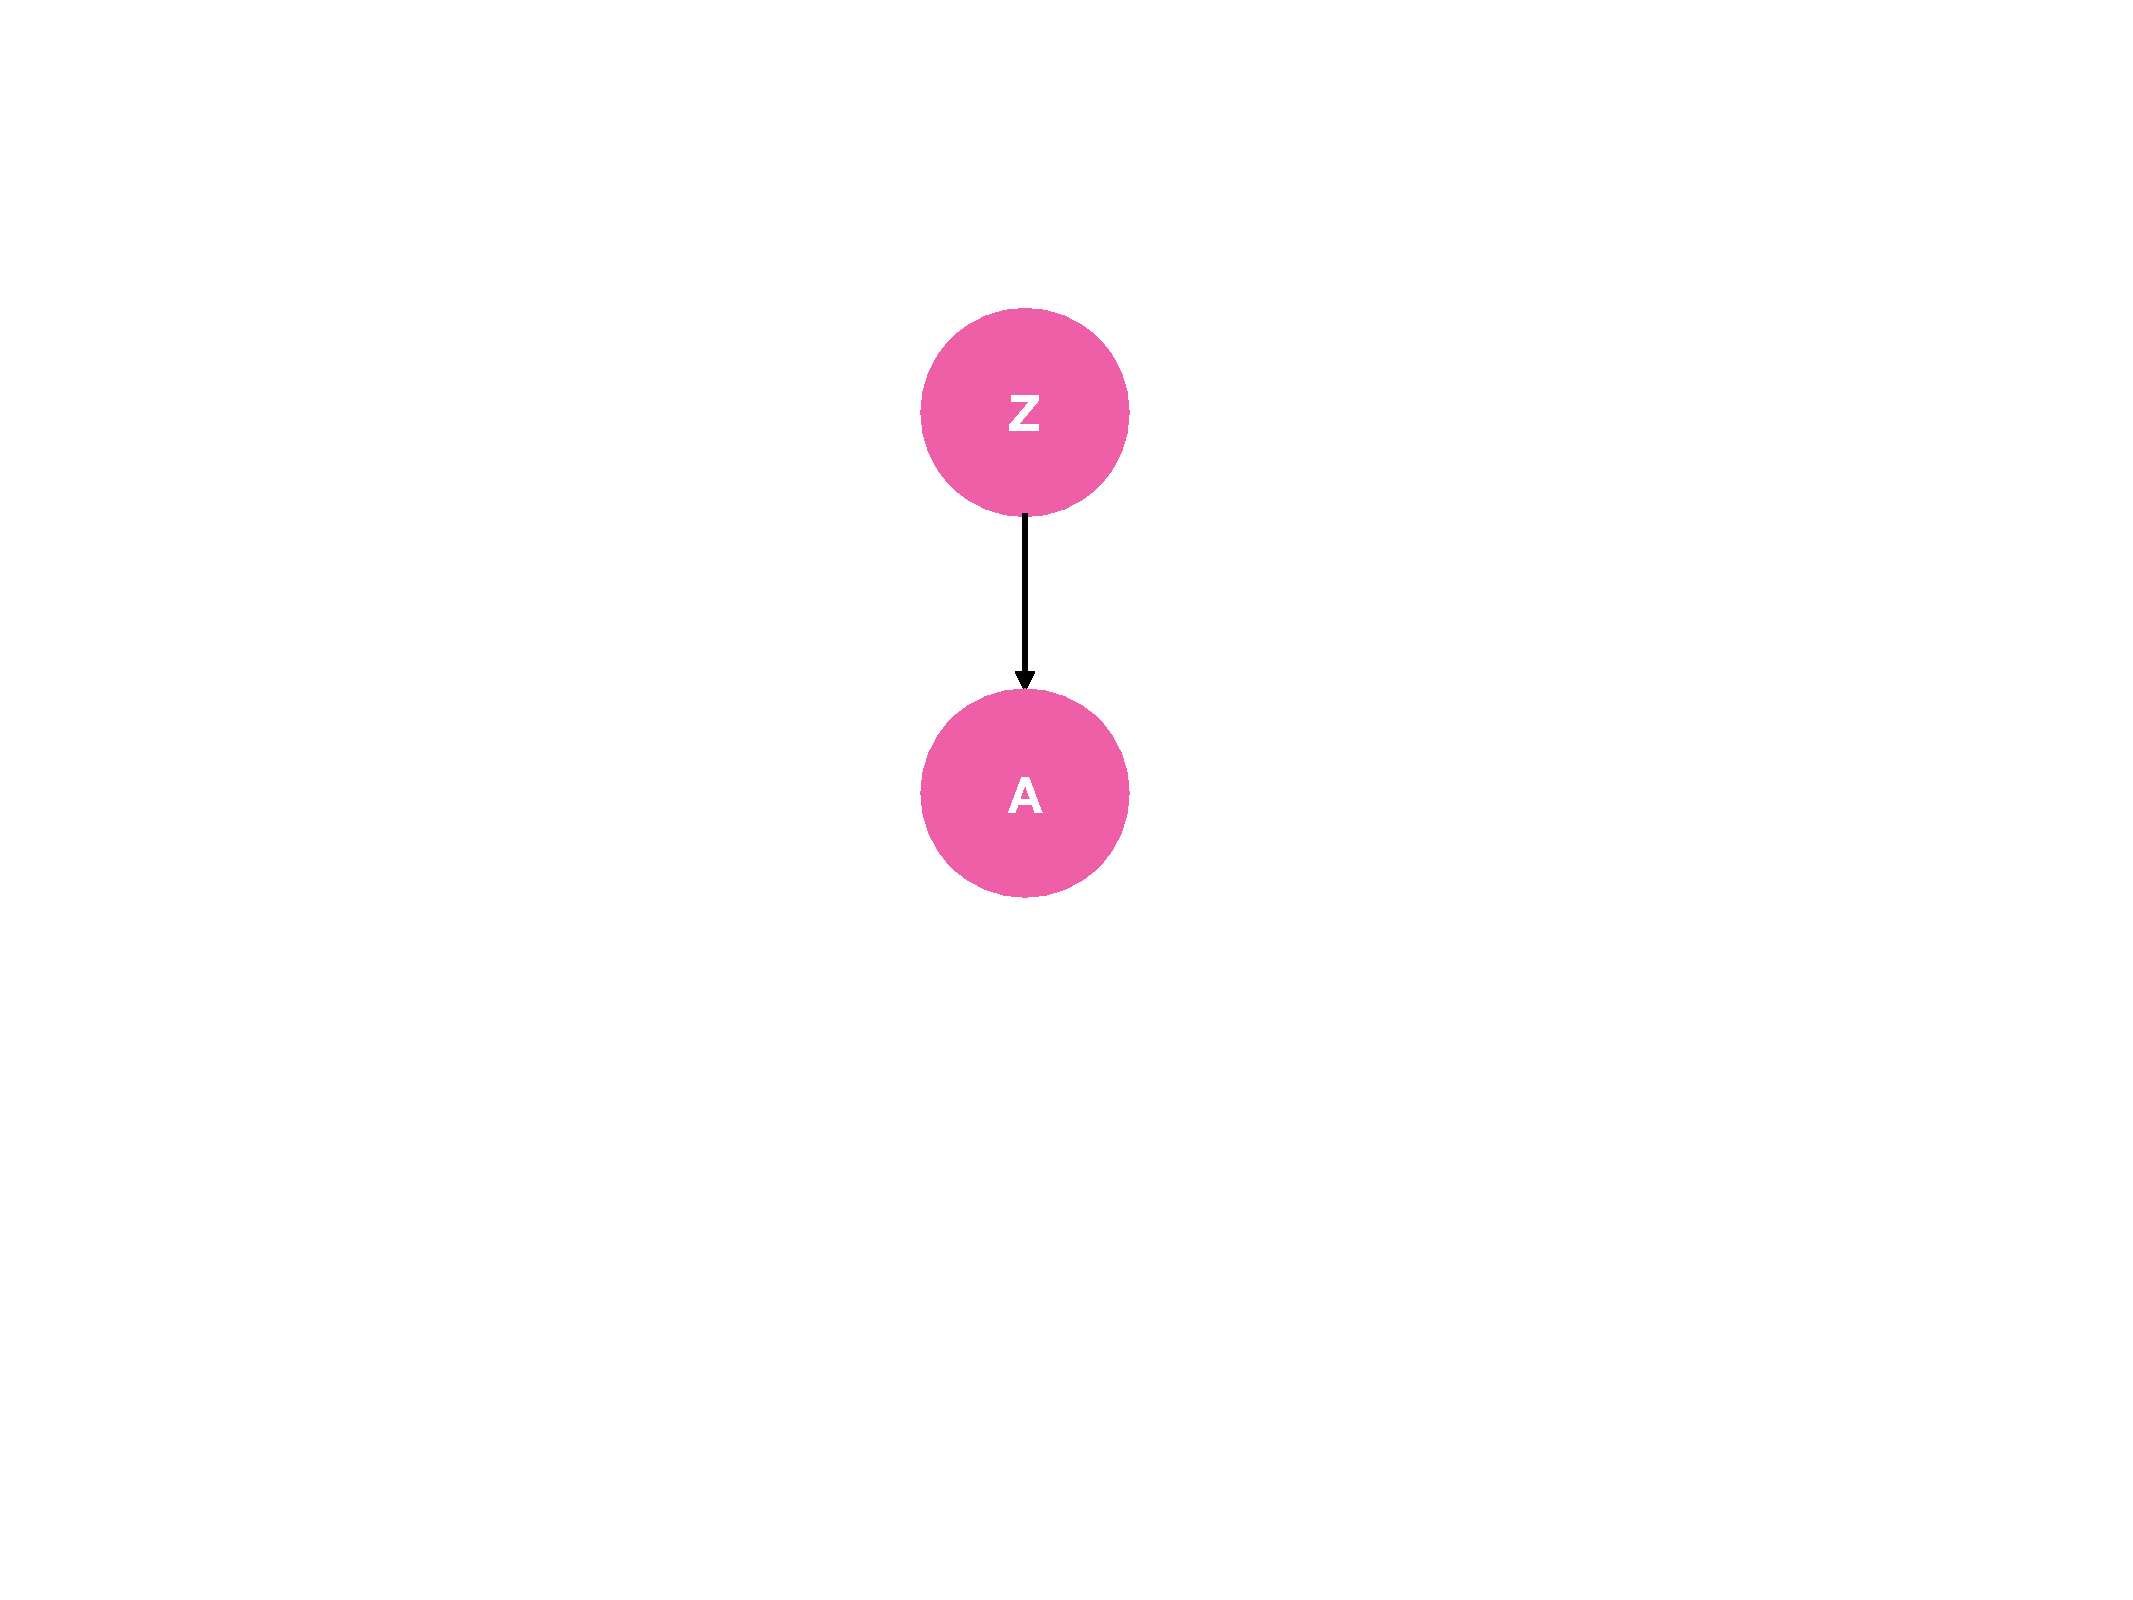
\includegraphics[scale=0.3]{SBMGraphical}
\caption{{\bf SBM Graphical Model.} A graphical model is used to model the dependency between the node-to-community assignments, ${\bf z}$ and the observed network adjacency matrix, ${\bf A}$.}
\label{fig:graphical}
\end{center}
\end{figure}

Using the factorization rules described in section \ref{pgm}, we can specify the complete data log likelihood between ${\bf z}$ and ${\bf A}$ as,

\begin{equation}
\log P({\bf z},{\bf A})=\log(P({\bf A} \mid {\bf z}))+\log(P({\bf z}))
\end{equation}

To further specify these communities, we will define additional notation. First, let ${\boldsymbol \pi}_{K \times K}=\{\pi_{ij}\}$ be the matrix that specifies the within and between community edge probabilities. Using this information, we can model the probability of an edge existing between nodes $i$ and $j$ as,

\begin{equation}
P(a_{ij}=1)\sim \text{Bernoulli}(\pi_{z_{i},z_{j}}).
\end{equation}

Here, $\pi_{z_{i},z_{j}}$ is the connection probability between the inferred community assignments of nodes $i$ and $j$. 

Further, we let $Z_{i}=\{Z_{i1},Z_{i2}, \dots Z_{ik}\}$ be a collection of binary indicators where $Z_{ik}$ is 1 $i$ belongs to community $k$ and 0 otherwise, We also let $\alpha_{k}$ be the probability that a node belongs to community $k$. With all of this information, we can write down each term of the complete data likelihood.

First,

\begin{equation}
\log(P({\bf Z}))=\sum_{i}\sum_{k}Z_{ik}\log(\alpha_{k}).
\end{equation}

Next,

\begin{equation}
\log(P({\bf A} \mid {\bf Z}))=\sum_{i\ne j}\sum_{k< l}Z_{ik}Z_{il}[a_{ij}\log (\pi_{kl})+(1-a_{ij})\log(1-\pi_{kl})]
\end{equation}

Optimizing the parameters of this incomplete data log likelihood requires computing the posterior $P({\bf z} \mid {\bf A})$ but unfortunately is intractable, as shown by Daudin \emph{et al.} \cite{dudin}. To address this issue, the posterior can be recast using a factorized approximation. This is accomplished by optimizing a lower bound of $\mathcal{L}({\bf A})$. We let $\mathcal{R}_{A}$ be an approximation of the posterior, $P({\bf z} \mid {\bf A})$. To optimize the lower bound of $\mathcal{L}(\mathcal{A})$, we seek the $\mathcal{R}_{A}$ that is as close as possible to $P({\bf z} \mid {\bf A})$. In other words, we define the lower bound of $\mathcal{L}({\bf A})$ as $\mathcal{T}(\mathcal{R}_{A})$, with,

\begin{equation}
\mathcal{T}(\mathcal{R}_{A})=\log \mathcal{L}({\bf A})-\text{KL}[\mathcal{R}_{A}(\bf z), P({\bf z} \mid {\bf A})].
\end{equation}

Here KL denoted the Kullback-Leibler divergence (KL divergence) and the best approximation will be the value that makes the KL divergence the smallest. Jaakkola \emph{et al.}, present a mean field approximation for the posterior distribution \cite{jakk} as,

\begin{equation}
\mathcal{R}_{A}({\bf z})=\prod_{i}h(Z_{i};{\boldsymbol \tau}_{i}).
\end{equation}

Here ${\boldsymbol \tau}=(\tau_{i1}, \dots, \tau_{iK})$ and $\tau_{ik}$ is the approximation that node $i$ belongs to community $k$, or $P(Z_{ik}=1 \mid {\bf A})$. Furthermore, $h(\cdot;{\boldsymbol \tau}_{i})$ denotes the multinomial distribution with parameter ${\boldsymbol \tau}$. 

Daudin \emph{et al.}  \cite{dudin} , show that the optimal estimate for $\tau_{ik}$ denoted $\hat{\tau}_{ik}$ satisfies

\begin{equation}
\hat{\tau}_{ik} \propto \alpha_{k}\prod_{j \ne i}\prod_{l}[\pi_{z_{i},z_{j}}^{a_{ij}}(1-\pi_{z_{i},z_{j}})^{1-a_{ij}}]^{\hat{\tau}_{ik}}.
\end{equation}

Here, $\alpha_{k}$ notes the probability that a node belongs to community $k$. Furthermore, after computing the set of variational parameters, the updates for ${\boldsymbol \alpha}$ and ${\boldsymbol \pi}$ that maximize $\mathcal{T}(\mathcal{R}_{A})$ are also shown by Daudin \emph{et al.,} \cite{dudin} to be,

\begin{equation}
\hat{\alpha}_{k}=\frac{1}{n}\sum_{i}\hat{\tau}_{ik}  \hspace{.5in}  {\theta}_{ql}=\sum_{i \ne j}\hat{\tau}_{iq}\hat{\tau}_{jl}a_{ij}/\sum_{i \ne j}\hat{\tau}_{iq}\hat{\tau}_{jl}
\end{equation}

We have presented this variational approach for performing SBM parameter inference and likelihood optimization because this approach was appropriate for the work presented in this thesis. Variational inference is just one approach that can be applied to learn model parameters and was but a study by  Zhang \emph{et al.} \cite{comp} also show that belief propagation \cite{belief} is very effective for this task. Briefly, belief propagation is a message passing algorithm for parameter inference in probabilistic graphical models. Given that parameter learning offer requires computing marginal distributions for a set of variables with a very large number of possible configurations, belief propagation uses the graphical model to reduce the complexity of the problem.  

This formulation of the problem and parameter optimization procedure works well and converges quickly for networks that have assortative community structures and a homogenous degree distribution. We will now explore how this classic formulation of the SBM can be modified to enable a broader application for a variety of networks.

\subsubsection{Variants to the Classic Stochastic Block Model}

The introduced stochastic block model is the most vanilla version in that it makes the assumption that the network is unweighted and that each node is assigned to only one community. The introduced model also does not account for issues that may arise from degree heterogeneity (i.e. a wide degree distribution).  Here, we will briefly discuss the approaches that adapt the stochastic block model to handle these issues and assumptions. 

{\bf Edge Weights}

\indent The majority of the stochastic block model literature considers unweighted networks simply because describing a probabilistic model to handle both edge existence and edge weight is a challenging task. In the classic stochastic block model, we are simply modeling whether an edge exists based on the inferred community memberships of the edge stubs. Since edge weights can come in a variety of forms (real-valued, count, etc.), it is difficult to immediately decide what distribution the edge weights should follow. In the past few years, this issue has been tackled in two papers \cite{aicher,peix}.

\indent First, Aicher \emph{et al.} developed a model and associated inference technique as the initial efforts toward a weighted stochastic block model. Here, edge weights can be modeled by any exponential family probability distribution. The authors use a mixing parameter that allows for the control of the use of edge existence versus edge weights when learning node-to-community assignments. This method requires an estimate for the number of expected communities, $K$. However, the paper provides an approach to use Bayes' factors between two competing values of $K$ to determine which model is a better fit. The inference for fitting this model is performed through a variational bayes approach \cite{vBayes}.

\indent To avoid having intuition about $K$, Peixoto \cite{peix} developed a non parametric bayesian approaches that is capable of inferring $K$ with no prior knowledge. The assumption of the model is also slightly different and assumes a hierarchical structure between communities. The inference is achieved through Markov Chain Monte Carlo (MCMC) sampling. 

{\bf Degree Heterogeneity}\\
\indent Based on the variety of network structures and types, the assumption that the classic stochastic block model is an appropriate model for even classic unweighted data is often invalid. That is, for some networks, the fitted model may not actually be a good fit, in that samples from the learned model are substantially different from the network. Work by Karrer \emph{et al.} \cite{degreecorrectSBM}, introduced a simple extension to the classic stochastic block model, known as the degree corrected stochastic block model. This model is informed by degree distribution as a proxy for the network structure. In networks where there is a wide degree distribution (i.e. many high degree nodes and many low degree nodes), stochastic block models inference tends to partition the nodes into communities of high degree and low degree nodes. The approach for adapting the SBM to this setting is to slightly modify the learned $K \times K$ matrix, ${\boldsymbol \pi}$ slightly. Here, $\pi_{ij}$ described the number of edges between nodes $i$ and $j$. Further, these edges counts are modeled as poisson random variables. The likelihood of the observed network under this poisson assumption takes into each node's degree. 

{\bf The restriction of single community membership}\\
\indent As it is often observed in social networks, the assumption that every node belongs to only a single community is restrictive. To address this issue, approaches have been developed to  allow nodes to  participate in a mixture of communities \cite{mixMember} or be members of overlapping communities \cite{LA}. Airoldi \emph{et al.}, pioneered the development of the mixed membership stochastic block model \cite{mixMember}, where instead of modeling a node's membership in each community in a binary manner, the authors allow a node to belong to multiple communities. The generative process for this approach for modeling the existence of an edge between nodes $p$ and $q$ in a network with $K$ possible communities and the $K \times K$ matrix, ${\boldsymbol \theta}$ representing the between community connection probabilities.

\begin{itemize}
\item For each node $p$, draw a mixed membership vector $\pi_{p}\sim \text{Dirchelet}({\boldsymbol \alpha})$
\item Then for each pair of nodes $(p,q)$, draw ${\bf z}_{p\rightarrow q} \sim \text{Multinomial}(\pi_{p})$, ${\bf z}_{q\rightarrow p} \sim \text{Multinomial}(\pi_{q})$
\item Sample the edge between $p$ and $q$ as, $A_{pq}$, where $A_{pq} \sim \text{Bernoulli}({\bf z}_{q\rightarrow p}^{T}{\boldsymbol \theta}{\bf z}_{q\rightarrow p})$
\end{itemize} 

Following the development of the mixed membership stochastic block model, Latocuhe \emph{et al.} \cite{LA} addressed an important limitation of \cite{mixMember}. Since the probability of an edge between a pair of nodes $p$ and $q$ depends on a single draw of ${\bf z}_{p\rightarrow q}$ and ${\bf z}_{q\rightarrow p}$, the class memberships of nodes $p$ and $q$ towards other nodes in the network are ignored. Moreover, this model adapts the mixed membership stochastic block model to incorporate a higher order resolution of structure by considering each node in the context of its neighbors. 

\subsubsection{Affiliation model and inference}

We have previously discussed extensions of the stochastic block model that account for the assumption that nodes can belong to multiple communities. Another interesting idea is the idea of \emph{pluralistic homophily}, where the probability that two individuals are connected is related to the affiliations of the nodes \cite{pluralHom}. In other words, the more groups a pair of nodes share, the more likely they are to have a connection. For example, if two two people were graduate students, studying computational biology at the same university, they are more likely to be connected than a pair of graduate students studying different subjects at the same university. A state-of-the-art method called BIGCLAM was presented for this task by Yang \emph{et al.} in 2013 \cite{bigclam}. The objective here is to model the connection probability between a pair of nodes based on the similarity in their learned affiliations towards communities. To do this, individual nodes are connected with communities with some number of links, with more links from a node to a community indicating that the node has a higher `affilation' to that group. For a network with $N$ nodes and $c$ communities, the affiliation between nodes and communities is encoded by a matrix, ${\bf F}$, where $F_{uc}$ is the learned count of links (again encoding the affiliation), between node $i$ and community $c$. Similarly, let $F_{u}$ and $F_{v}$ be the community affiliations for nodes $u$ and $v$. Then the probability that an edge exists between nodes $u$ and $v$, or $P(A_{uv}=1)$ is modeled as, 

\begin{equation}
P(A_{uv}=1)=1-\exp(-F_{u}F_{v}^{T}).
\label{eqAff}
\end{equation}

The node to community affiliations can be used as a proxy for the total amount of interaction between a pair of nodes $u$ and $v$ with a Poisson distribution. This modeling paradigm will for the straightforward modeling of the probability that an edge exists between the node pair. To do this, the total amount of interaction between nodes $u$ and $v$ is modeled as,

\begin{equation}
X_{uv}=\sum_{c}X_{uv}^{c}, X_{uv}^{c} \sim \text{Poisson}(F_{uc}\cdot F_{vc}).
\end{equation}

The convenience of this model lies in the fact that we also know how to handle the sum of Poisson random variables is distributed ($X_{uv} \sim \text{Poisson}(\sum_{c}F_{uc}\cdot F_{vc})$), and corresponds to equation shown in \ref{eqAff}. From here, it is straightforward to model the probability of $u$ and $v$ sharing connections based on the Poisson probability mass function as,

\begin{equation}
P(X_{uv}>0)=1-P(X_{uv}=0)=1-\exp(-\sum_{c}F_{uc}\cdot F_{vc})
\end{equation}

From here the task is then to learn the ${\bf F}$ that maximizes the log-likelihood ($ll$) of the observed network, ${\bf A}$, $ll({\bf F} \mid {\bf A})$. This can be expressed (in terms of the set of edges, $E$) as,

\begin{equation}
ll({\bf F})=\sum_{(u,v) \in E} \log(1-\exp(-F_{u}F_{v}^{T}))- \sum_{(u,v) \notin E} F_{u}F_{v}^{T}.
\end{equation}

This optimization problem can be easily solved with a block coordinate gradient ascent algorithm, which updates the $F_{u}$ for each $u$, while keeping all other $v$ fixed. Ultimately, after ${\bf F}$ has converged, there needs to be a rule to decide which communities $u$ is a member of. To do this, some threshold is chosen, $\delta$ such that now $u$ belongs to community $c$ if $F_{uc}>\delta$. BIGCLAM was shown to outperform competing methods, such as the mixed membership stochastic block model on large social networks with ground truth communities. 


\subsection{Deep Learning Approaches}
\indent In recent years, deep learning has begun to revolutionize many fields, including network analysis. Perozzi \emph{et al.}, pioneered the use of deep learning in community detection with the development of DEEPWALK \cite{deepWalk} to learn a latent space representation of nodes in some $d$-dimensional Euclidean space (i.e. an emedding). Once the network is embedded in a lower dimensional space, simple clustering techniques, such as $k$-means \cite{kMean} can be used to partition the network into communities. The approach to learn an embedding for the network is based on random walks on the network \cite{rWalk,gleichpagerank}. A random walk on a network involves choosing a starting node and traversing the network by hopping between adjacent nodes. The DEEPWALK approach seeks to learn an embedding of the nodes that preserves the sets of nodes traversed in a random walk. To do this, the authors adapted the Word2Vec approach to this context. Word2Vec is a powerful tool from natural language understanding that allow for the specification of a node embedding that enables accurate prediction of a word's context, given the word \cite{word2Vec}. To adapt this context to networks, a random walk is treated as a sentence and nodes are treated as a word within the sentence. Moreover, the analogous task to the problem in text data to a network is to accurately predict a set of nodes likely to be seen on a random walk with the node of interest. The embeddings should preserve these learned rules. Moreover, this problem is solved using the same optimization approach as Word2Vec \\
\indent Based on the success of DEEPWALK, the method was followed up with Node2Vec in 2016 \cite{node2vec}. While node2vec also uses the random walk framework to specify the optimization problem, they modify how the random walk is performed to enable an embedding that captures different aspects of a potential network community. For example, one may describe a community by a set of nodes located close to each other in the network with many common neighbors and connections to common neighbors. This assumption is known as network homophily \cite{homophily}. Alternatively, perhaps a good definition of a community is a set of networks that have similar roles in the network. This idea is known as structural equivalence \cite{structural}. For example, a community under structural equivalence might group could group nodes with similar degree or centrality. To modify the random walk so that it leads to a model that gives flexibility in the nature of retrieved communities, the authors introduced a search bias term, which controls whether the random walk in performed in a breadth-first or depth-first search parameter. If on a random walk, the path is traversed in a depth-first search, favoring the exploration of a larger area of the network far from the random walk source, the resulting community aligns with the homophily hypothesis. A random walk performed in a breadth first manner that restricts the path to nodes neighboring the source and tends to capture nodes based on structural equivalence (i.e. a hubs, high degree nodes, or low degree nodes). 

\subsection{Higher order network analysis}
One of the most recent advances in community detection is clustering nodes based on `higher order' features, or at the level of small subgraphs or \emph{motifs}. The structural organization of the network is then interrogated by identifying clusters of network motifs. The flexibility and appeal of this framework is that different kinds of organizational patterns of the network can be identified, depending on the motif used. Seminal work using this approach was proposed by Benson \emph{et al.} \cite{Benson} . Given a motif, $M$, higher order clustering frameworks seek to identify a cluster of nodes $S$ that minimize the following ratio,

\begin{equation}
\phi_{M}(S)=\text{cut}_{M}(S,\bar{S})/\min(\text{vol}_{M}(S),\text{vol}_{M}(\bar{S})),
\end{equation}

where $\bar{S}$ denoted the set of nodes not in $S$, $\text{cut}_{M}(S,\bar{S})$ is the number of instances of motif $M$ with a least one node in $S$ and one node in $\bar{S}$. Finally, $\text{vol}_{M}(S)$ is the number of nodes in instances of $M$ that belong to $S$. The optimization framework to identify near-optimal clusters is an extension to standard spectral clustering methods and it outlined as follows. 
\begin{enumerate}
\item For a motif of interest, $M$, define a motif adjacency matrix, $W_{M}$ where the $ij$th entry is the the number of instances of $M$ that contain nodes $i$ and $j$
\item Compute the spectral ordering (i.e. order the eigenvalues in descending order), $\delta$, of the nodes from the normalized motif Laplacian of $W_{M}$. Note this motif Laplacian is the standard Laplacian matrix for $W_{M}$ \cite{laplacian}. 
\item Identify the set of $\delta$ with the smallest motif conductance, or, $S := \arg \min_{r} \phi_{M}(S_{r})$, where $S_{r}=\{\delta_{1}, \dots, \delta_{r}\}$. 
\end{enumerate}

The novelty in this approach stems from the fact that it can be applied to a variety of network types that not all methods can handle. In particular, Benson \emph{et al.}, highlight how this approach can be used to deal with directed, undirected, weighted, unweighted, and signed networks \cite{Benson}, as well as the flexibility to uncover diverse types of structural organization. 

\section{Community detection in computational biology}
Analyzing networks with community detection has shown to be fruitful, particularly in biology and neuroscience applications. In this section, we will describe examples of analyses where the identification of communities provided insight and understanding for a biological problem. 

Multiple experimental modalities exist that enable the collection and analysis of biological data. Understanding protein expression, gene expression, microbiome composition, metabolomic profiles, genomic mutations, and immune profiling are just a few of examples of biological data that is studied routinely for insight into human health. With most experimental platforms producing high dimensional data, it is crucial to have good tools for interpretation, visualization, and prediction. Machine learning techniques in computational biology have revolutionized prediction in biology and medicine \cite{systemsImmuno,deepGenome,machineGenomics}. In this section, we outline particular examples of how the application of community detection to diverse types of biological data lead to improved scientific understanding and predictive ability.

\subsection{Immunological profiling to establish a pregnancy immune clock}
A study lead by Aghaeepour \emph{et al.}, demonstrated that there is a typical timing of immunological events in a healthy, term, human pregnancy \cite{immuneClock}. Immunological profiling was performed on a training cohort of 18 women, using a technology called mass cytometry \cite{cytof} was used to quantify various features of the immune system, such as, cell type abundances and signaling activity. A correlation network between the measured set of immune features in the training cohort was constructed to develop hypotheses about their interactions. In addition to the construction of the network, an elastic net regression model \cite{eNet} was trained to identify immune features associated with increased gestational age. When communities were identified in the correlation network of the immune features, there were two important observations. First, immune features of the same type (i.e. cell signaling vs. cell frequency) were aligned with community labels. Second, sets of features associated with a particular gestation age often fell in the same community, indicating their synchronous activity during a particular time in the pregnancy. Finally, after identifying influential nodes in their ability to predict stage in pregnancy, according to the regression model, the communities of these nodes were more closely examined to uncover further insight into the immunological mechanisms occurring throughout the pregnancy time course. 

The use of community detection in this analysis helped to understand which immune features and combinations of immune features are predictive of increased gestational age. The implications of such an observation is an increased ability to predict when a pregnancy is diverting from its normal, healthy progression. 

\subsection{Uncovering differences in microbiome community structure in patients with inflammatory bowel disease}

\indent The microbiome refers to the collection of bacterial species that populate an organism's gut. Microbiome analysis has recently gained attention, as its biological implications are large for health and disease \cite{gut}. A 2017 review article presented the idea that the development of network analysis approaches for microbiome data is under explored and has great potential for advancing biological understanding and interpretation of these data \cite{networkMicrobiome}. A network in this context is typically constructed based on some notion of co-occurence or correlation between microbial species, profiled across samples. A recent example where community detection played a key role in the biological understanding was introduced in 2017 and assessed the interplay between microbial co-occurence structural organization patterns between patients with and without inflammatory bowel disease \cite{moduleMicrobiome}. Communities were identified in the healthy and diseased networks, using classic modularity maximization \cite{girvancommunity}. After identifying a community structure for each network, the similarity of these partitions was quantified with the Rand index \cite{Rand}, which showed to be statistically significant under a permutation test. This observation allowed the authors to understand that the core structure from a healthy microbiome was conserved even in diseased patients, but allowed for more careful probing of the subtle differences. First, the functional roles of the members in each community were interrogated. Some interesting co-occurence relationships within communities were identified, such as the loss of strong clustering, or association propensity between pro and anti-inflammatory species within the diseased networks. This interplay between pro and anti inflammatory species is thought to play a pivotal role in the maintenance of a healthy gut microbiome. \\
\indent Next, the authors used the community structure of each network to study the differences in node roles (i.e. importance) between the healthy and IBD networks. Within the neuroscience community, there have been numerous efforts to characterize nodes, in terms of the role they play connecting communities or as an important node within a community \cite{hub}. Nodes have the potential to be \emph{connecters}, where they have high `participation' or connections with many nodes across numerous communities. Alternatively, a node can be an intramodular hub, where it serves as a high degree node, connecting to many members of its community. After assessing the role of each node in the healthy versus IBD network, the roles of many nodes were not consistent between the two networks. Most notably, the most prominent community-connector nodes in the healthy network were lost in the IBD network. Further, there were some nodes with few intermodule connections in the healthy network, that increased their role as a connector node in the IBD case. The interrogation of nodes with a dramatic change in their role are good candidates for follow-up investigation. \\
\indent Overall, the partitioning of each network into communities allowed for a systematic comparison between the healthy and disease network and to prioritize specific species (nodes) and co-occurence patterns for further investigation. 

\subsection{Community detection for analysis of flow cytometry data}
\indent Flow cytometry allows for the the simultaneous quantitative analysis of a large population of cells within a biological sample. Typically, cells are strained with fluorochrome-conjugated antibodies which emit light upon encountering laser beams in the flow cytometry machine. This emitted light is measured and reported as a quantitative measurement of the cell. An important analysis of flow cytometry data is the ability to automatically group cells based on their similarities in light emission and quantification \cite{flow}. While this process was historically performed manually, there has been a significant amount of work to develop computational methods that can successfully segment cell populations, automatically \cite{nimaFlow}. A network-based approach to this problem, known as SamSPECTRAL was introduced in 2010 by Zare \emph{et al.} \cite{FlowSpectral}. In this approach, the authors seek to segment a population of cells into distinct subpopulations, through the construction of pairwise single cell similarity network. After constructing this network, communities detection can be applied to cluster the cells into sub populations. To recap, in this network, the nodes are comprised of the individual cells within a sample, and edges between nodes indicate the similarity between a pair of cells, based on the quantification of their emitted light. Another useful feature of SamSPECRAL is that it also does some preprocessing to reduce the size of the constructed network.

\indent To create a network of the flow cytometry data, a large subset of data points (cells) are first sampled and denoted as `registered' nodes. The next step is to look at the collection of `unregistered nodes' and ultimately assign them to their closed registered node neighbor. Iteratively, the unregistered nodes are attempted to be registered or agglomerated with the set of registered nodes. For example, for one of the registered nodes, which can be denoted as $p$, the set of unregistered nodes within some defined distance $h$ become registered to $p$.  The set of unregistered nodes that were newly assigned to be registered are removed from the set of unregistered nodes. This process is repeated until there are no more unregistered nodes. Each set of nodes registered with the same label are denoted as a community (an inconvenient label, given a network will be constructed and communities will be identified). A weighted network is constructed between these registered communities with edge weights quantifying the similarity in the quantitative features (as quantified through flow cytometry) between a pair of a communities. Once this weighted graph is created, a spectral community detection method \cite{spectral1} is applied to segment the network into 1 of $K$ network communities. These is one final post-processing step, motivated by previous work in computational flow cytometry methods,  to combine the agglomerate a pair of network communities if members if the community show similarity greater than a predefined threshold (in terms, again, of their measured flow cytometry properties). The usefulness of this approach is that it exhibited outstanding performance on datasets containing clusters of challenging shapes. Some examples of challenging shapes are, overlapping clusters, non-elliptical shaped clusters, or low-density clusters. Ultimately the retrieved population of cells avoided manual segmentation and provided a solution to a computationally challenging task.

\subsection{Understanding genetic diversity of the malaria parasite genes}
\indent Rich genetic diversity in the  \emph{var} genes of the human malaria parasite has been shown to contribute to the complexity of the epidemiology of the infection and disease. The parasite can change which of the  \emph{var} genes are expressed at any given time on the infected red blood cell, which prevents the antibody from recognizing and resisting the new protein. One diversity-generating mechanism is recombination, which is the exchange and shuffling of genetic information during mitosis and meiosis \cite{varIntro}. The ability to understand genetic diversity is complicated by inadequate tools to uncover the phylogeny, or genetic relationship between sequences resulting from recombination events, in a scalable and statistically rigorous way. The typical analyses for evolutionary data assume a tree-like relationship between events, which is unrealistic for recombination data. To address this challenge, \cite{larremoreparasite} use a novel approach: they cast their problem in terms of a collection of networks. Then, they apply community detection to each of the networks and use the properties of the communities to generate hypotheses of the mechanisms behind the recombination process. To investigate the heterogeneity and the corresponding possible patterns in recombination events across a set of 307 sequences from the \emph{var} gene, the authors restricted their analyses to 9 particular ``highly variable regions'' (HVR) within each of the 307 sequences. Then for each HVR, they constructed a network, where the nodes represented the 307 sequences and an edge was placed between a pair of nodes if they had evidence of a recombinant relationship, based on a notion of sequence similarity within the particular HVR. Communities were then identified in each of the 9 networks using a degree-corrected stochastic block model (SBM) approach \cite{degreeCorrect}.\\
\indent After identifying communities within each HVR network, the authors used two summary statistics to formulate their biological hypothesis. First, the variation of information \citep{VI} was used to compare the community assignments of nodes (i.e.\ each of the 307 sequences) across the 9 HVR networks. They observed that each network had a prominent community structure (i.e.\ far from random) and that the community assignments between networks were quite distinct. These observations motivated the hypothesis that recombination events occur in constrained ways, leading to a strong community structure, and that one should analyze HVR networks individually instead of building a consensus network that aggregates the HVR networks.  Next, they used \emph{assortativity} \cite{newmanAssort} to overlay the network structure with various known biological features of the sequences, such as  \emph{var} gene length. Specifically, assortativity quantifies the tendency of nodes of the same type (e.g. same gene length) to be connected in the network. They observed that three HVR networks had community structure correlating strongly with two biological features (i.e. nodes of the same biological label tend to group together), while three other HVR networks with highly heterogenous community structure were unaligned with any of the known biology. These observations allowed for the formulation of the hypothesis that the HVRs that are unrelated to each other also promote recombination under unrelated constraints and are responsible for fostering genetic diversity to avoid immune evasion. \\

\indent Given the ability to find communities within each HVR network and the lack of similarity in community structure between HVR networks, \cite{larremoreparasite} were able to formulate and test hypotheses for the diversity-generating mechanisms of \emph{var} genes, and this would have been difficult using standard phylogenetic approaches or without adopting a community-based perspective. The application of the stochastic block model to this task provided a statistically grounded approach for testing the plausibility of the model.

\subsection{Analysis of high dimensional single cell data for tumor heterogenity}
\indent A very beautiful application of community detection is the development of a network and community detection based method, called PhenoGraph for the analysis of single cell data \cite{phenoGraph}. Single cell technologies allow for the profiling of cells individually within a sample. Recent attention and methods development have focused on the use of RNA sequencing and mass cytometry for high dimensional profiling of single cells. Single cell technologies have enabled for an advancement in the understanding of the pathobiology of cancer in that cells within a tumor have been shown to exhibit a large amount of heterogeneity at the single cell level. Furthermore, this heterogeneity has important functional and clinical significance \cite{intraTumor}. The data produced by these single cell technologies profiles millions of cells, based on multiple features (whether those be genetic, immunological, or signaling response). Moreover, a key challenge is to accurately separate individual cells into biologically meaningful subpopulations or cell phenotypes. While we will mostly profile the community detection based method used for this task, the implications of this work lead to the identification of a cellular phenotype and a corresponding gene expression signature which was highly correlated with accurate prediction of patient survival rates. 

\indent Unsupervised analysis of cell types is a challenging problem as there are millions of cells, with each cell being a point in $d$-dimensional space. Traditional clustering algorithms are too slow, or require assumptions about the number of clusters, or the shape of the data in high-dimensional space. One benefit of community detection on networks is that many methods do not require specification of the number of clusters and are agnostic to the shape of the data in high dimensions. The first step of PhenoGraph is to build a $k$-nearest neighbor network between pairs of cells. To do this, each cell is connected to its $k$-nearest neighbors. The second step of the algorithm refined the $k$-nearest neighbor network to prioritize keeping the most similar pairs of nodes connected in the network and removing extraneous connections. This is done by creating a new weighted network between the cells based on the Jaccard similarity measure. In this context, the Jaccard similarity between a pair of nodes reflects the similarity of their neighbors in the network. With this refined network, modularity based community detection was applied and each of the resulting communities corresponds to a distinct cellular phenotype. When this method was applied to a manually gated (i.e. cells were manually separated dataset),  PhenoGraph showed very strong performance for multiple values of $k$. The authors specifically tried, $k=\{15,30,45,60\}$. 

The authors also provide an approach to add supervision to the problem, which uses partially labeled data set. In this context, this means that some of the cells have a classification. Moreover, given that the network contains $N$ nodes, with $T$ labeled nodes ($T<L$), the objective is to label the remaining $N-T$ nodes. Based on a concern that network-based classification methods operating on a majority vote rule for a node's neighbors, the authors sought to develop an approach that would not suffer in circumstances where a node's closest neighbors were a small subset of the available labeled data. This issue is mediated through the use of label information on the whole network through a random walk. Conceptually, starting from an unlabeled node, the random walker can move through the network, taking into account edge weight information at each step. The random walk classification scheme from an unlabeled node is therefore the probability of its random walk ultimately arriving at a node from each of the classes.  The probability of an unlabeled node reaching a node in each of the labeled classes can be computed in a straightforward way, using the graph laplacian \cite{RWR}. \\
\indent Overall, the findings of this paper use community detection to allow for the analysis and understanding of tumor heterogeneity data that was not possible with standard high dimensional data analysis techniques.  The authors suggest that this method is useful in characterizing primitive cancer cells and for the identification of cell biology features that define particular biological states and clinical outcomes. 

\subsection{Identification of virulence factor genes related to antibiotic resistance of uropathogenic \emph{E. coli}}
\indent Urinary tract infections are primarily caused by uropathogenic \emph{E. coli} (UPEC). In their study Parker \emph{et al.,} seek to better understand UPEC antibiotic resistance, which prevents patients from being treated for urinary tract infections. Using a cohort of 337 \emph{E. coli} patient isolates, the authors looked closely at the virulence factor genes of these patients. Virulence factors are non conserved or are carried on mobile genetic elements and elicit biological functions that relate to uropathogenesis (i.e. the onset of a patient getting at UTI). The biological function of virulence factors are known and allow for the development of therapeutic agents. In the analysis, the presence or absence for each of 16 virulence factors was determined. A network was constructed between the 337 patient isolates, with each edge reflecting the pairwise similarity in their virulence factor profiles. Modularity based community detection was then applied to this network and partitioned it into 4 different communities. Most remarkably, each of the 4 communities was characterized by clinical isolated described by either a single or pair of virulence factor markers. These pairs of related virulence factors were then probed further to investigate their role in antibiotic resistance. This approach offers a n ew way to integrate genomic and individual patient information to determine which types of antibiotics might be most effective.  

\section{Thesis Contribution}
In the previous section, we presented several case studies for how community detection enables and simplifies biological understanding. To recap, a network representation data and a community detection analysis can help to uncover structural organizational patterns and important co-occurence relationships in applications, such as, immunology and microbiome analysis. Further, community detection enables clustering, even if the task seems computationally challenging, or has complicated geometry in high dimensions. While previous work in community detection is well-developed for standard networks modeling a single type of relational definition between nodes, we find it necessary to adapt these approaches to more diverse types of network data.  

\subsection{Thesis Statement}
In this thesis, we address three challenging types of network data,  where the identification of communities is challenging. Among these classes of networks, we have developed four new methods that adapt standard community detection to these situations. {\bf 1) We focus on how to identify communities in multilayer networks through an extension of the stochastic block model.} Our method learns a collection of models to describe the entire multilayer network. {\bf 2) We provide a method to pre-process a large network into a smaller network of \emph{super nodes} that can be used as input to a community detection algorithm.} This pre-processing step decreases the run time of community detection algorithms and decreases the variability across multiple runs of the community detection algorithm. {\bf 3) We extend the stochastic block model to handle attributed network data, which allows the inference of node-to-community assignments to handle both connectivity and continuous attribute information.} Our learned model for the connectivity and attributes can be used to perform link prediction and collaborative filtering.  {\bf 4) We develop a test to generate an empirical $p$-value to quantify the extent to which attributes and connectivity align.} Our approach is based on label propagation and we use synthetic data and a single cell mass cytometry dataset to validate the empirical $p$-value generated by our test.

\subsection{Summary of the novelty of this work}

 To succinctly summarize the contributions of this thesis, we outline each of the 3 developed methods, their top 3 pieces of related work, and why our approach makes a novel contribution in table \ref{Tab11}. 
\begin{table}[h!]
\tiny
\begin{tabular}{ p{3cm}||p{3cm}|p{3cm}|p{3cm} }
 \multicolumn{4}{c}{} \\
%\hline
 Method& Brief Description & 3 Similar Approaches & Novelty\\
 \hline
sMLSBM (Chapter 2)   & Stochastic block model for multilayer networks  & MLSBM through aggregation methods \cite{catala}, Restricted MLSBM \cite{mlsbm1},  MLSBM \cite{airoldi} & Instead of fitting a consensus SBM to all layers, we learn a set of models that represents different clusters of layers.\\
\hline
SuperNode (Chapter 3) &  Pre-processing a network into a smaller network of super nodes before applying community detection  & Identify communities on core of network and propagate labels outward \cite{peng}, Create super nodes with prior information about nodes expected to be together \cite{SuperNodeSide}, Reduce the size of the network by systematically removing nodes and edges \cite{gilbert}  & We recast the entire network as a network of super nodes and input this smaller version into community detection algorithms. We do not require prior knowledge or side information\\
\hline
Attribute SBM (Chapter 4) & Incorporate both network connectivity and continuous attributes into account when assigning nodes to communities  & SBM inference with a single attribute \cite{clauset}, iLouvain Modifying modularity to incorporate attributes \cite{ilouvain}, CESNA: Affiliation model with attributes \cite{cesna} & We adapt the SBM to handle multiple continuous attributes\\
 \hline
Attribute Alignment Test (Chapter 5) & A test to quantify the extent to which attributes and connectivity align.  & neoSBM + BESTest (attribute augmented SBM) \cite{peel2017ground}. To our knowledge, there are not any related tests other than \cite{peel2017ground} & We use label propagation to generate an empirical $p$-value that quantifies how the attributes relate to connectivity. We do not require assuming that a stochastic block model is an appropriate representation of the network.\\
\hline
\end{tabular}
\caption{{\bf Summarizing the novelty of our 3 developed methods}. For each of the 3 methods we developed, we provide a brief description of what it does, the top 3 most similar approaches, and why our approach is novel.}
\label{Tab11}
\end{table}
\subsection{Relevant Publications}
The work addressed in this thesis can be found in the following publications. note that we have organized the publications by the theme they address. \\

{\bf Community detection in multilayer networks}
\begin{enumerate}
\item \emph{Clustering Network Layers with the Strata Multilayer Stochastic Block Model}. {\bf N. Stanley, S. Shai, D. Taylor, P.J. Mucha}. IEEE Transactions on Network Science and Engineering. 2016. \url{http://ieeexplore.ieee.org/abstract/document/7442167/}
\item \emph{Enhanced Detectability of Community Structure in Multilayer Networks Through Layer Aggregation}. {\bf D. Taylor, S. Shai, N. Stanley, P.J. Mucha}. Physical Review Letters. 2016. \url{https://journals.aps.org/prl/abstract/10.1103/PhysRevLett.116.228301}
\end{enumerate}

{\bf Community Detection (General)}
\begin{enumerate}
\item \emph{Case Studies in Network Community Detection.} {\bf S. Shai, N.Stanley, C Granell, D. Taylor, P.J. Mucha}. Appears as a chapter in the Oxford Handbook of Social Networks. 2017. \url{https://arxiv.org/abs/1705.02305}
\end{enumerate}

{\bf Pre-Processing for Community Detection in Large Networks}
\begin{enumerate}
\item \emph{Compressing Networks with Super Nodes}. {\bf N. Stanley, R. Kwitt, M. Niethammer, P.J. Mucha}. Under Review. 2018. \url{https://arxiv.org/abs/1706.04110}
\end{enumerate}

 {\bf Community Detection for Attributed Networks}
 \begin{enumerate}
 \item \emph{Stochastic Block Models with Multiple Continuous Attributes}. {\bf N. Stanley, T. Bonacci, R. Kwitt, M. Niethammer, P.J. Mucha}. In preparation. 2018. 
 \end{enumerate}
 
 \subsection{Software}
 The four developed methods described in this thesis are available and maintained in github. 
 
 \begin{enumerate}
 \item {\bf sMLSBM: Fitting a multilayer stochastic block model}. \url{https://github.com/stanleyn/sMLSBM}
 \item {\bf SuperNode: For compressing a large network}. \url{https://github.com/stanleyn/SuperNode}
 \item {\bf Attributed SBM: For fitting an SBM with multiple continuous attributes}. \url{https://github.com/stanleyn/AttributedSBM}
 \item{\bf AttributeAlign: For testing alignment between attributes and connectivity}. \url{https://github.com/stanleyn/AttributeAlign}
 \end{enumerate}
 
%%%%%%%%%%%%%%%%%%%%%%%%%%%%%%%%%%%%%%%%%%%%%%%%%%%%%%



\chapter{A multilayer stochastic block model}
In this chapter we present the strata multilayer stochastic block model (sMLSBM). The sMLSBM method and inference described here is described in \emph{Clustering Network Layer with the Strata Multilayer Stochastic Block Model} \cite{smlsbm}. The goal in developing this method is two-fold. First, we seek to develop an approach to cluster network layers within a multilayer network. Second, we wish to develop a novel extension to the stochastic block model to handle the information contained across network layers and determine which subsets of the network layers are are likely to be samples from the same stochastic block model. 

\section{Introduction to multilayer networks}
Currently, we are relatively comfortable working with a single network of nodes and edges, capturing one type of relational definition. We have seen this numerous times thus far in this thesis, from modeling similarity of immune features in women during pregnancy to profiling microbiome species co-occurence patterns in patients with IBS. With the consistently improving ability to generate and analyze large amount of biological data, there is often the opportunity to generate multiple relational definitions between a set of objects. This could be simply the desire to compare a gene co-expression network across multiple tissues \cite{ohmNet}, or the desire to study multiple microbial co-occurence networks in different sites of the body \cite{microbiome}. Multilayer networks provide a framework to do this, in that each relational definition leads to a new layer in the network \cite{kivelamultilayer,boccaletti2014structure,manlioMathFoundations}.  Such data and corresponding networks have shown to be useful in many contexts, such as, in the comparison of genetic and protein-protein interactions in a cell \cite{genetic}, in understanding underlying relationships and community structure across social networks \cite{socialnetwork}, and in the analysis of temporal networks \cite{muchamultislice}. Furthermore, recent advances in the mathematical foundations for multilayer networks have made analysis of these types of data more feasible. In particular, \cite{manlioMathFoundations} has introduced a mathematical formalism with tensors. Doing so allows for the calculation of important network quantities, such as centrality and clustering coefficients, as well as modularity \cite{muchamultislice}. Thus, given the inherent multiplexity of network data across fields as well as recent theoretical developments for handling these types of data, there exists a need for the development of appropriate tools that can leverage information from all layers to elucidate structural patterns.

\indent Inspired by the ideas in \cite{domen} that groups of layers often provide redundant information, we seek to further explore this idea to identify sets of layers, which we denote as ``strata", with each stratum described by a single probabilistic model based on community structure.  This effectively amounts to defining \emph{local} probabilistic network models, and is analogous to biclustering \cite{biclustering} or co-clustering \cite{cocluster} problems. Moreover, our method can be regarded as a joint clustering procedure, in which the nodes and layers of networks are clustered simultaneously. Just as in \cite{cocluster}, where the objective is to jointly cluster words and documents such that joint word-document subgroups correspond to particular topics, our objective is to cluster network layers such that each stratum is a set of layers with a characteristic community structure. To achieve this goal, we have developed the strata multilayer stochastic block model (sMLSBM). We additionally emphasize that by collectively utilizing similar layers in a principled way, we can achieve more robust community detection and parameter inference for the probabilistic community detection models that describe each stratum. 

\section{Comparing network layers based on community structure}
\indent The problem of aggregating layers in a multilayer network is closely related to the problem of clustering networks. That is, given an ensemble of networks, one aims to identify sets such that networks within a set have similar characteristics. 
These characteristics, or ``features'' in this context, can describe any of the following: micro-scale structural properties such as subgraph motifs \cite{ugander2013subgraph,motiffinding}; multiscale properties such as community structure \cite{taxonomy,NONCluster,confusingMesoscopic}, the spectra of network-related matrices \cite{structurenetwork} and by defining latent roles \cite{netensemble}. Although clustering layers in a multilayer network is closely related to clustering networks in an ensemble, these are distinct problems with different difficulties and nuances. We focus on the prior pursuit; however, we expect for certain network ensembles that it will be beneficial to modify and apply our methods to the clustering of networks. 
%These include subgraph motifs \drt{\cite{scalablemotif,motiffinding}}, community structure \cite{taxonomy}, multiscale properties such as topological summaries [dane], and network summary statistics \cite{netensemble,structurenetwork}.
\\
\indent 
In this work, we analyze and compare layers in a multilayer network based on their community structure. Community detection in single-layer networks is an essential tool for understanding the organization and functional relatedness between nodes in a network \cite{porter2009communities,fortunato}.
Although there are many definitions for what constitutes a ``community'' \cite{rombach2014core}, one often assumes an ``assortative community'' in which there is a prevalence of edges between nodes in the same community as compared to the amount of edges connecting these nodes to the remaining network. In seeking to identify such communities, numerous approaches have been proposed, including those based on
%Identifying communities in networks typically requires the identification of the best partitioning of nodes into groups to maximize number of within-community edges, which can be quantified by multiple approaches, such as 
maximizing a modularity measure \cite{newmanmodularity} and fitting a generative probabilistic model \cite{abby}. Because each of these approaches present computational challenges for efficiently detecting communities, numerous heuristics exist for developing practical algorithms \cite{community,fortunato,leskoveccommunity,clausethierarchy,newmanspectral}. \\
\indent While our approach is to define a probabilistic model for multilayer community structure, we note that there have previously been approaches to understand similarities in network ensembles that are grounded in exploiting similarities in community structure between networks. In \cite{NONCluster}, the authors seek to partition a group of networks into subgroups through construction of a network of networks (NoN). Communities in the NoN are chosen such that the networks representing the nodes are sufficiently similar in their underlying community structure. In one significant application of this method, the authors clustered gene co-expression networks and found an increased number of significant functional enrichment categories for biological processes. Similarly, in \cite{confusingMesoscopic}, the authors explore mesoscopic similarity between layers using an informational theoretic approach. While they have designed their method to handle any feature of network architecture, they highlight their ability to quantify similarity between network layers based on node-to-community assignments in the layers. \\
%
%
%In this research we compare networks based on their community structure. Specifically, 
\indent In seeking a statistically-grounded approach for studying communities in multilayer networks, we consider the stochastic block model (SBM) \cite{originalSBM}, a popular generative model for community structure in networks. The assumption of the SBM is that nodes in a particular community are related to nodes within and between communities in the same way, thus allowing SBMs to describe several types of communities (e.g., assortative, disassortative, core-periphery, etc. \cite{rombach2014core,aicher}). 
%
There are many other appealing aspects of stochastic block models; for example, a model-based approach allows for the denoising of networks through the removal of false edges and the addition of missing edges \cite{abby,guimera2009missing}.
%
As we introduced in chapter 2, the inference procedure for fitting SBMs to an undirected network with $N$ nodes and $K$ communities involves learning the two parameters, ${\boldsymbol \pi}$ and ${\bf Z}$. Parameter ${\boldsymbol \pi}$ is a $K \times K$ symmetric matrix, where $\pi_{mn}$ gives the probability of an edge existing between a given node in community $m$ and another node in community $n$. Matrix ${\bf Z}$ is an $N \times K$ indicator matrix, wherein each binary entry $Z_{im}$ indicates whether or not node $i$ is in community $m$. Each row of ${\bf Z}$ is constrained such that $\sum_{m=1}^{K} {Z}_{im}=1$, i.e. each node only belongs to 1 community. We also define vector $\boldsymbol z$, which has entries $z_{i}=\text{argmax}_m \{Z_{im}\}$ that indicate the community to which node $i$ belongs. For a given network, these parameters are often inferred through a maximum likelihood approach, and once learned, they provide information about the within and between community relatedness. 

\section{Related work in community detection of multilayer networks}
Due to the ubiquity of network data with multiple network layers, community detection in multilayer networks constitutes an important body of research. Important directions include generalizing the modularity measure \cite{muchamultislice} and studying dynamics \cite{manlio2} for this more general setting. 

Given the usefulness of SBMs for the understanding of node organization in single-layer networks, it is important to extend SBMs to the multilayer framework, and indeed this direction of research is receiving growing attention  \cite{airoldi,mlsbm1,barbillon,catala,thiagomlsbm}. In this context, the general assumption is that there are shared patterns in community structure across the layers of a multilayer network, and the goal is to define and identify a stochastic block model that captures this structure. These works have explored many types of applications that can arise involving multilayer networks,
%
and have therefore given rise to several complementary models for multilayer stochastic block models (MLSBMs). We now briefly summarize this previous work that is very related, but notably different, from the model we study herein.
%
%Specifically, research thus far focused on two problems: one has a given network with many layers, or one has a single layer that is assumed to be derived from some aggregation of the layers. 
\\\indent 
 In Refs.~\cite{airoldi,mlsbm1,barbillon}, the authors studied situations in which many layers follow from a single SBM. In these instances, it is possible to obtain improved inference of the SBM parameters by incorporating multiple samples from a single model. For example, in Ref.~\cite{airoldi} the authors considered an increasing number of layers, $L$, and explored asymptotic properties of the estimated SBM parameters. Specifically, they fit an SBM to each individual layer in a way that utilizes the information from all layers, and they showed convergence of these estimators to their true values as $L\to\infty$. %As expected, as the number of layers increases, so does the quality of inference. 
For a network with $L$ layers and $K$ communities in each layer, their approach requires  an estimate of the community assignment matrix ${\bf Z}^l$ and probability matrix ${\boldsymbol \pi}^l$ for each layer $l$, the latter of which involves learning $K(K+1)L/2$ parameters.To this end, the authors extended the variational approximation for approximating the maximum likelihood estimates of SBM parameters introduced in single-layer SBMs introduced in \cite{Dudin} to the multilayer setting.
\\\indent Ref.~\cite{airoldi} was followed up by Ref.~\cite{mlsbm1}, wherein the authors addressed issues that can arise for the model when $K$ and/or $L$ is large, or if the network is sparse.They proposed a modified model called the restricted multilayer stochastic block model (rMLSBM). 
In this model, instead of learning a set of $L$ independent parameters, ${ \pi}^l_{mn}$, for each pair, $(m,n)$, each entry in ${\boldsymbol \pi}$ is fully layer-dependent so as to produce a reduction in the number of free parameters. Specifically, to determine the probability of an edge between a node from community $m$ and a node from community $n$ in layer $l$, they use a logistic link function and model the probability as $\text{logit}({ \pi}_{mn}^{l})={\pi}_{mn}+\beta_{l}$. The $\beta_{l}$ is an offset parameter representing the particular layer or type of edge. In this model, it is necessary %in an $L$ layer \drt{network} with \drt{$K$} communities
to learn $K(K+1)/2+L$ total parameters. Thus, the maximum likelihood estimate for an rMLSBM is a regularized estimator.\\
\indent  Consistent with the theme of fitting a single block model to a collection of layers, Ref.~\cite{barbillon} is similar to Refs.~\cite{airoldi} and \cite{mlsbm1} in that the authors seek to leverage information from all layers by considering the joint distribution of layers. Using this, they estimated quantities such as the marginal probabilities of node assignments to communities and the edge probabilities within and between groups. An interesting aspect of their approach is that they introduce a covariate capturing the coupling between pairs of nodes. For a network with $K$ communities and $L$ layers, this requires the estimation of $(2^{L}-1)K^{2}+(K-1)$ parameters. 
\\\indent We summarize Refs.~\cite{catala} and \cite{thiagomlsbm}, which provide techniques to determine whether a single layer network is the result of an aggregation procedure in a multilayer network. In Ref.~\cite{catala}, the authors defined a version of multilayer stochastic block model and an inference procedure for assessing whether or not a single-layer network was actually obtained from an aggregation of layers in a multilayer network; they considered the 
%they considered In particular, they \drt{seeked} to infer how network layer could have been 
aggregation of layers using boolean rules. Ref.~\cite{thiagomlsbm} describes two possible generative processes for multilayer networks: the \emph{edge-covariate} and \emph{independent-layer} models. In the edge-covariate model, an aggregated network is defined in which a given edge $(i,j)$ only appears in a single layer. Aggregating the layers in a multilayer network into a single network representation combines all of the edges from each of the layers. Thus, the translation of this idea into a generative model involves choosing a layer membership for each edge and sampling edges with a probability conditioned on adjacent nodes. In the independent-layer model, layers are generated independently from each other and the only constraint is that group membership of the nodes are the same across all layers. \\
\indent While motivation to pursue this problem originated from \cite{domen}, we point out that our approach does not provide a method for aggregating layers or reducing the number of layers in the network. Instead, it can in a sense compress the network in that the learned stochastic block model parameters for each stratum can be used to generate a sample network to serve as a consensus for that stratum. 

\section{A Summary of Novel Contributions of sMLSBM}
\indent 
While the literature on MLSBMs has recently grown quickly, there is still a need for a probabilistic generative model that allows for the layers in a multilayer network to be described by multiple SBMs. To this end, we
developed a novel multilayer stochastic block model, sMLSBM, that assigns network layers into disjoint sets that we call strata, where a collection of layers in a given stratum are assumed to be samples from the same underlying generative model. Our method can be viewed as a joint clustering procedure, where we seek to group layers into strata and nodes into communities. That is, we seek to simultaneously find layer-to-strata and node-to-community assignments. 

In order to address practical applications that can involve multilayer networks with several strata, layers, communities and nodes, we introduce an algorithm that effectively partitions layers into strata and an inference procedure to learn the SBM parameters for each stratum. Importantly, these two steps---assigning nodes to communities and layers to strata---are combined in an iterative algorithm so that an improvement in community detection can lead to an improvement in the clustering of layers into strata, which can iteratively lead to further improvement in community detection, and so on.
%
\begin{figure}
\begin{center}
\label{goals}
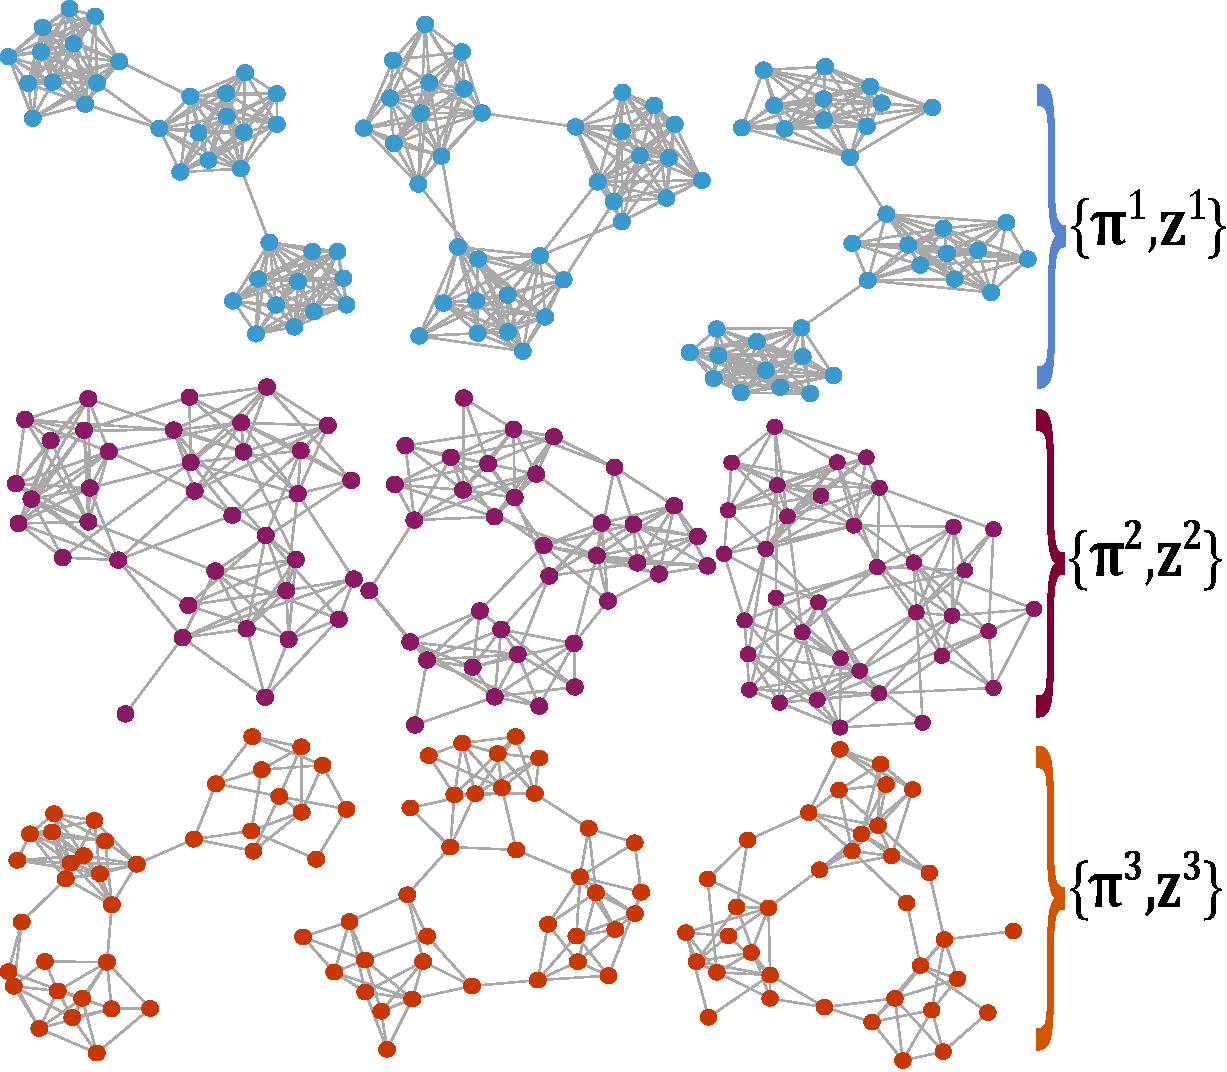
\includegraphics[width=.5\linewidth]{Figure_1.pdf}
%\includegraphics[width=1\linewidth]{FIGS
\caption{{\bf Objective of strata multilayer stochastic block model (sMLSBM)}. Each of the $L=9$ networks here represents a layer in a multilayer network. Every network layer has $N=36$ nodes that are consistent across all layers. There are $S=3$ strata as indicated by the three rows and the colors of nodes. Clearly, network layers within a stratum exhibit strong similarities in community structure. That is, although each layer follows an SBM with $K=3$ communities, the SBM parameters are identical for layers within a strata but differ between layers in different strata. We would like to partition the layers into their appropriate strata and learn their associated SBM parameters, $\pi^s$ and $Z^s$.}
\end{center}
\end{figure}

\section{sMLSBM Model Definition}
\indent Under the sMLSBM, the network layers, $G^{l}(N,\mathcal{E}^{l})$ are assumed to be generated by a set of $S$ stochastic block models, where the layers in stratum $s \in \{1,2,\cdots,S \}$, are parameterized by ${\boldsymbol \pi}^{s}$ and ${\bf Z}^{s}$ (or equivalently, vector ${\boldsymbol z}^s$, which has entries $z^s_{i}=\text{argmax}_m \{Z_{im}^s\}$ ). Note that the parameters ${\boldsymbol \pi}^{s}$ and ${\bf Z}^{s}$ for a single stratum are analogous in meaning to their respective parameters in the single-layer SBM case. 
 %
For each stratum $s$, we let $\mathcal{L}^s\subseteq\mathcal{L}$ denote the set of layers corresponding to $s$, so that $\mathcal{L}=\bigcup_s \mathcal{L}^s$ and $\emptyset=\mathcal{L}^s\cap \mathcal{L}^t$ for all $s,t\in\{1,\dots,S\}$, $s\neq t$. We let $L^s=|\mathcal{L}^s|$ denote the number of layers in strata $s$ so that $\sum_s L^s=L$.
Finally, we allow the number of communities, $K^{s}$, to vary across the strata.
\\\indent
 %Furthermore, since a stratum is composed of multiple network layers, the parameters represent a consensus for that group.
For a given multilayer network, our objective during inference is to identify the stratum assignment of each layer and to learn the collection of strata parameters, $\boldsymbol{\Pi}=\{\boldsymbol{\pi}^{1},\boldsymbol{\pi}^{2},\dots,\boldsymbol{\pi}^{S}\}$ and $\mathcal{Z}=\{{\bf{Z}}^{1},{\bf{Z}}^{2},\dots {\bf{Z}}^{S}\}$. The learned SBM parameters for a stratum represent a consensus for the associated layers, and so in that sense can be interpreted as reducing the effective number of layers \cite{domen}. However, strata can also be interpreted as a way to simply identify layers with similarities in community structure. Figure 1 shows a toy example of a multilayer network with $S=3$ strata, where each layer has $N=36$ nodes and $K=3$ communities. Each individual network in this figure represents a layer in the network. The nodes in the layers belonging to each stratum are colored according to their stratum membership; moreover, it is easy to see that layers of a stratum exhibit high similarities in community structure.  \\
  \indent As part of our procedure, we specify another parameter that we refer to as the adjacency probability matrix, ${\boldsymbol \theta}^{s}$, which can be computed from $\boldsymbol{\pi}^{s}$ and ${\bf{Z}}^{s}$. Specifically, ${\boldsymbol \theta}^{s}$ is an $N \times N$ matrix such that ${\theta}_{ij}^{s}$ gives the probability of an edge between nodes $i$ and $j$ in stratum $s$. That is, ${\theta}_{ij}^{s}={ \pi}^{s}_{z_{i}^{s}z_{j}^{s}}$, where  $z_{i}^{s}$ specifies the community number for node $i$ in stratum $s$. Finally, we define the matrix ${\bf Y}$ of size $L\times S$, wherein an entry $Y_{ls}$ is a binary indicator of whether or not layer $l$ is assigned to stratum $s$. Note that $\sum_{s}Y_{ls}=1$. We also define a vector $\boldsymbol y$, which has entries $y_{l}=\text{argmax}_s \{Y_{ls}\}$ to indicate the strata to which layer $l$ belongs.

\section{Inference for learning model parameters of sMLSBM}
\indent The procedure for fitting an sMLSBM to a given network requires finding the layer-to-strata memberships and node-to-community memberships that best describe the multilayer network. For notational convenience, we introduce hat notation to represent the learned parameter estimate from the inference procedure. We can write down the marginal likelihood for the collection of network layers, $\mathcal{G}$, as,
\begin{equation}
\label{eq1}
p(\mathcal{G}\mid {\boldsymbol \Pi})=\sum_{\mathcal Z}\sum_{{\bf Y}}p(\mathcal{G},{\mathcal Z},{\bf Y} \mid {\boldsymbol \Pi}).
\end{equation}
We assume the probability of an edge between two nodes in layer $l$ belonging to stratum $s$ can be modeled as a Bernoulli random variable, based on the community membership of the nodes. In particular, $p({A}^{l}_{ij}=1)\sim \text{Bernoulli}({\bf \pi}_{z_{i}z_{j}}^{s})$. \\
\indent Since ${\bf Y}$ and ${\mathcal Z}$ are both latent quantities, searching over all possible values quickly becomes intractable. To tackle this issue, we develop a two-phase algorithm that incorporates a clustering algorithm for choosing the best $\bf Y$. This greedy approach leads to a significant reduction for the size of the search space since only $\mathcal Z$ must be statistically inferred. Specifically, during Phase I, we infer an SBM for each layer in isolation, and we cluster together sets of layers that have similar SBM parameters. Using these results as an initial condition in Phase II, we develop an iterative method that jointly identifies layer-to-stratum and node-to-community assignments as well as the SBM parameters for each stratum. We provide a schematic of the algorithm in Fig.~\ref{fig:Schematic}, and below we present the two-phase algorithm in detail.

\noindent{\bf Phase I.}
Phase I is comprised of two parts. First, we fit an SBM to each individual layer $l\in\{1,\dots,L\}$, which yields inferred SBM parameters $\hat{{\boldsymbol \pi}}^l$ and node-to-community memberships $\hat{{\bf Z}}^l$.
Then we cluster the layers based on the similarities of $\hat{{\boldsymbol \pi}}^l$ and $\hat{{\bf Z}}^l$. To infer $\hat{{\boldsymbol \pi}}^l$ and $\hat{{\bf Z}}^l$, we use the the inference method described in \cite{Dudin}. Here, the authors used a variational inference technique to approximate the maximum likelihood estimates for the stochastic block model parameters. For the set of $L$ layers, this produces sets of SBM parameters for each layer, which we denote by $\hat{\boldsymbol{\Pi}}=\{\hat{\boldsymbol{\pi}}^{1},\hat{\boldsymbol{\pi}}^{2}, \dots, \hat{\boldsymbol{\pi}}^{L}\}$ and $\hat{\mathcal{Z}}=\{\hat{\bf{Z}}^{1},\hat{\bf{Z}}^{2},\dots \hat{\bf{Z}}^{L}\}$ (that is, at this stage of the procedure, each layer is temporarily treated as its own stratum). Note also that each $\hat{{\boldsymbol Z}}^l$ can be equivalently represented by vector $\hat{{\boldsymbol z}}^l$. Using the estimates $\hat{{\boldsymbol \pi}}^{l}$ and $\hat{{\bf Z}}^{l}$ for a given layer, $l$, we can construct the corresponding adjacency probability matrix, $\hat{{\boldsymbol \theta}}^{l}$, which is defined entry-wise by $\hat{{\boldsymbol \theta}}_{ij}^{l}=\hat{\pi}_{\hat{z_{i}},\hat{z_{j}}}^l$. Doing this for each layer results in a collection of adjacency probability matrices, $\hat{\boldsymbol{\Theta}}=\{\hat{\boldsymbol{\theta}}^{1},\hat{\boldsymbol{\theta}}^{2}, \cdots, \hat{\boldsymbol{\theta}}^{L}\}$.\\
\indent Now, we seek an initial partition of layers into strata based on $\hat{\boldsymbol{\Theta}}$. The goal is to identify $S$ sets $\mathcal{L}^s$ so that the matrices $\{\hat{\boldsymbol{\theta}}^{l}\}$ with $l\in\mathcal{L}^s$ are close to one another, but they are distant from the remaining matrices, $\{\hat{\boldsymbol{\theta}}^{l}\}$ with $l\in\mathcal{L}\setminus \mathcal{L}^s$.
%
%where the total distance across strata between the stratum consensus adjacency probability matrix and the adjacency probability matrices of stratum member layers is as small as possible. 
This is accomplished by treating each $\hat{\boldsymbol{\theta}}^{l}$ as a feature vector and applying $k$-means clustering with $S$ centers so as to identify $S$ strata, $\mathcal{L}^s$. Note that $S$ can be selected \emph{a priori}, or approximated with a measure such as the gap statistic \cite{gap}. This gives us an initial estimate $\hat{{\bf Y}}$ for ${\bf Y}$. Note that this procedure initially treats each layer as a separate stratum, but provides a principled agglomeration of layers into $S\le L$ strata.   

\begin{figure}
\begin{center}
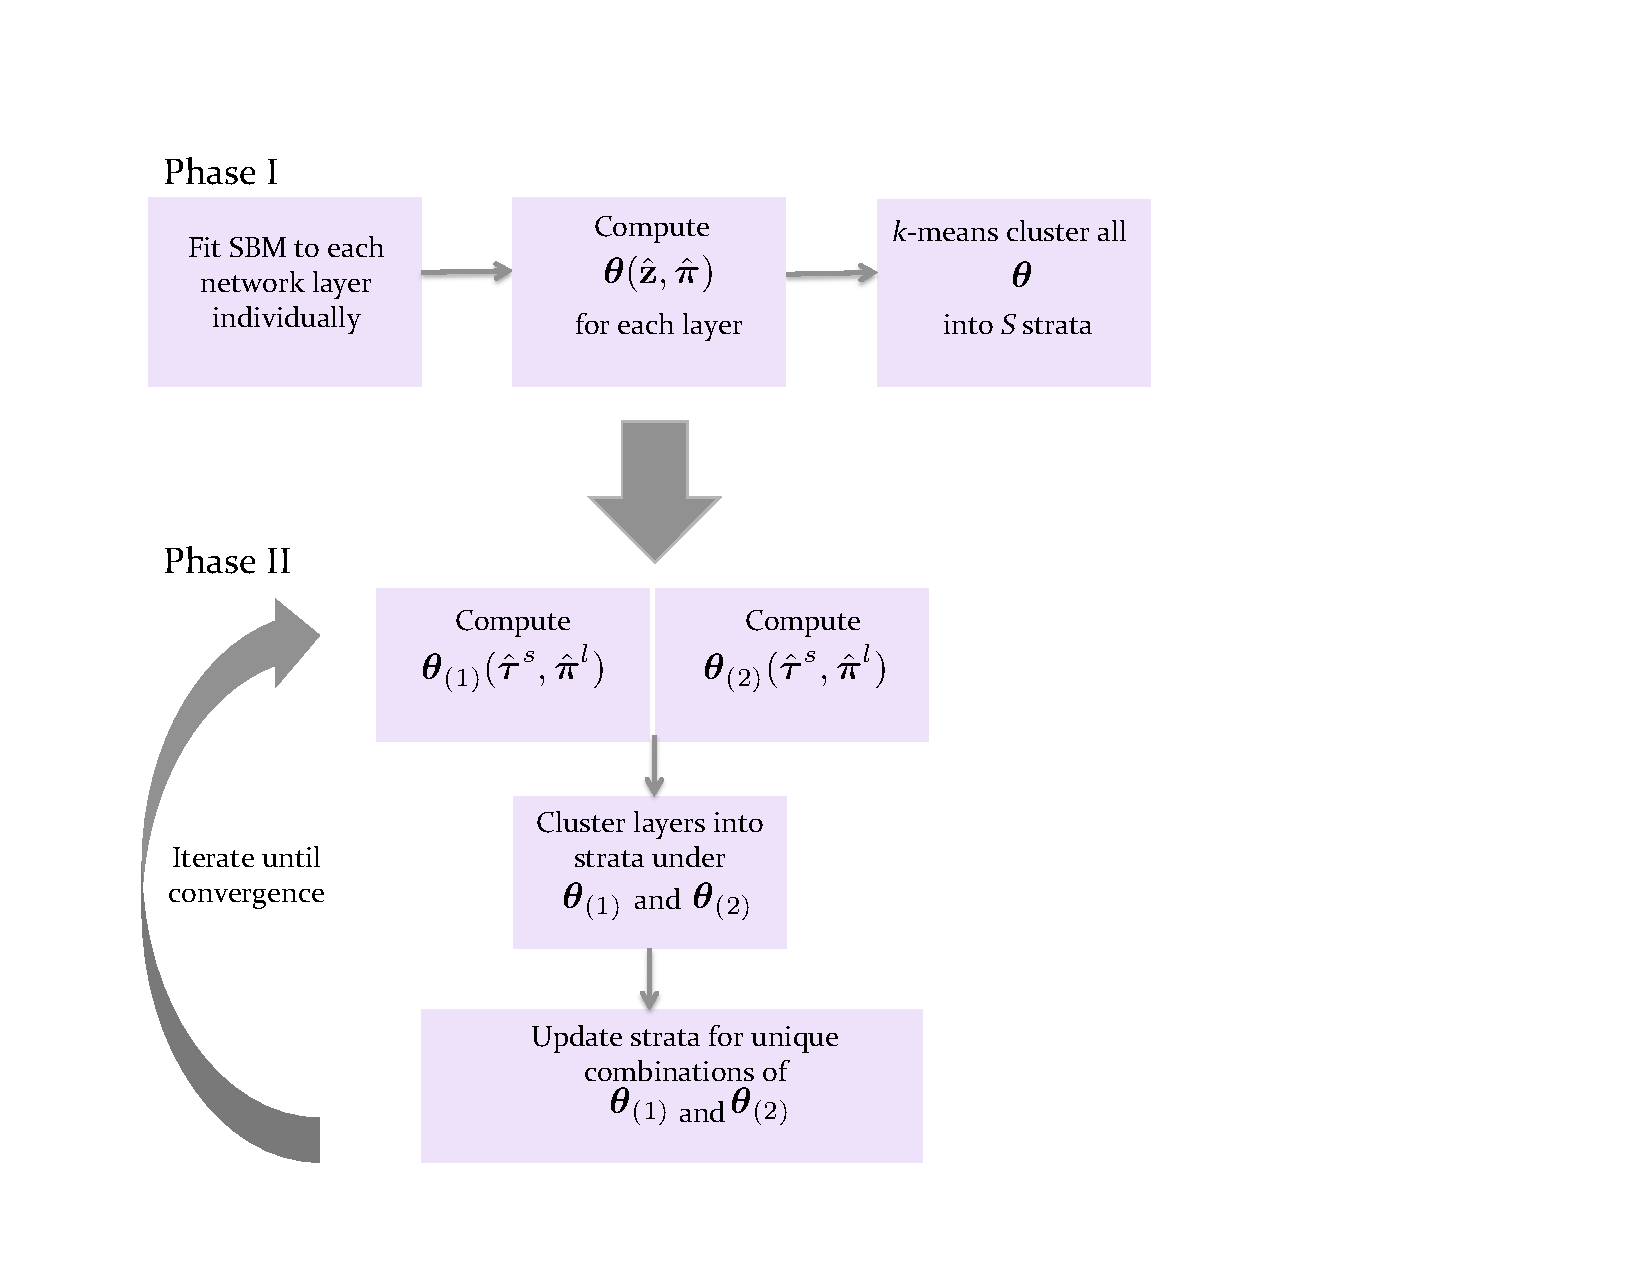
\includegraphics[width=.5\linewidth]{Figure_2.pdf}
\caption{{\bf Schematic illustration of our algorithm}: Our algorithm for fitting an sMLSBM is broken up into two phases: an initialization phase to cluster layers into strata, and an iterative phase that allows learning of node-to-community and layer-to-strata assignments.}
\label{fig:Schematic}
\end{center}
\end{figure}


\noindent{\bf Phase II.}
After a first-pass approach for assigning layers to strata, we initialize an iterative phase to more effectively estimate layer-to-strata assignments as well as the model parameters. Specifically, we would like to find the consensus SBM for each strata---that is, the $K^{s} \times K^{s}$ matrix $\boldsymbol{\pi}^{s}$ and the $N \times K^{s}$ matrix $\bf{Z}^{s}$ that maximize the likelihood of the observed layers in each stratum. We let ${\mathcal{A}}^{s}=\{{\bf A}^{l}\}$ for $l\in\mathcal{L}^s$ denote the collection of adjacency matrices corresponding to the $L^{s}$ layers in stratum $s$. 
%Hence each $\bf{A}$ is an $N \times N$ adjacency matrix. 

\indent We now proceed to maximize the likelihood in each stratum, by extending the framework of Ref.~\cite{dudin} to a multilayer context. Note that this is similar to Ref.~\cite{airoldi}, except that we are not aiming to infer an SBM probability matrix for each layer, individually. In particular, the complete-data log-likelihood for stratum $s$ can be written as,
\begin{equation}
p({\mathcal{A}}^{s},{\bf{Z}}^{s})=p({\mathcal{A}}^{s}\mid {\bf{Z}}^{s})p({\bf{Z}}^{s}),
\end{equation}
where
\begin{equation}
p({\mathcal{A}}^{s} \mid {\bf{Z}}^{s})=\prod_{l \in \mathcal{L}^{s}}\prod_{i< j}\prod_{mn}{{{\pi}}^{s}_{mn}}^{A^{l}_{ij}}(1-{{\pi}}^{s}_{mn})^{(1-A_{ij}^{l})}.\
\end{equation}
To write $p({\bf{Z}}^{s})$, it is helpful to introduce a new parameter $\alpha^{s}_{m}$ that represents the probability that a randomly-selected node in stratum $s$ belongs to community $m$, i.e. $\alpha^{s}_{m} = p({{Z}}^{s}_{im}=1)$. 

Note that $\sum_{m} \alpha^{s}_{m} =1$. 
%Further, we let $\mathcal{L}^{s}$ be the set of layers belonging to stratum $s$. 
Using this parameter, we can write
\begin{equation}
p({\bf{Z}}^{s})= \prod_{i}\prod_{m}\alpha{_{m}^{s}}^{({Z}^{s}_{im})}.
\end{equation}
%
It follows that the complete-data log-likelihood for the adjacency matrices representing the layers in stratum $s$ can be expressed as,
%
\begin{equation}
\begin{split}
\log P({\mathcal{A}}^{s},{\bf{Z}}^{s})&=\log(P({\bf Z}^{s}))+\log(P(\mathcal{A}^{s}\mid {\bf Z}^{s}))\\
&=\sum_{i}\sum_{m}{{Z}}^{s}_{im}\log(\alpha^{s}_{m})\\
&+\sum_{l \in \mathcal{L}^{s}}\sum_{i< j}\sum_{mn} A^{l}_{ij}\log({{\pi}}^{s}_{mn}) \\
&+\sum_{l \in \mathcal{L}^{s}}\sum_{i< j}\sum_{mn}(1-A^{l}_{ij})\log(1-{\pi}^{s}_{mn}).\
\end{split}
\end{equation}

Problems of this variety that involve the need to compute maximum likelihood estimates with incomplete data are typically addressed with the expectation maximization (EM) framework \cite{dempster}. Doing so requires the ability to compute $P({\bf{Z}}^{s}\mid{\mathcal{A}}^{s})$;  however, Ref.~\cite{dudin} showed that it is intractable to calculate the conditional distribution for the single-layer network case. To address this challenge, we use a variational approximation, analogous to approaches in  \cite{airoldi,barbillon,dudin}. In general, a variational approximation seeks to optimize a lower bound on the log-likelihood. To do this, we first approximate the conditional distribution, $P({\bf{Z}}^{s}\mid{\mathcal{A}}^{s})\approx{R}_{\mathcal{A}^{s}}$, where
\begin{equation}
R_{\mathcal{A}^{s}}({\mathbf Z}^{s})=\prod_{i}h({\mathbf Z}_{i\cdot}^{s};{\boldsymbol \tau}_{i\cdot}).
\end{equation}
Here, matrix ${\boldsymbol \tau}^{s}$ contains entries $\tau^{s}_{im}$ that approximate the probability that node $i$ belongs to community $m$ in stratum $s$. Further, function $h(\cdot)$ represents the multinomial distribution, with parameters, $\{{\boldsymbol \tau}^{s}_{im}\}$ for $m\in\{1,\dots,K^s\}$. Using this, we define the variational approximation as
\begin{equation}
\mathcal{J}(R_{\mathcal{A}^{s}})=\ell \ell(\mathcal{A}^{s})-\text{KL}(R_{\mathcal{A}^{s}}({\bf Z}^{s}),P({\bf Z}^{s}\mid \mathcal{A}^{s})),
\end{equation}
%
where $\ell \ell$ is log likelihood and KL is the Kullback-Leibler divergence. 

Through maximizing $\mathcal{J}(R_{\mathcal{A}^{s}})$, we minimize the KL divergence between the true conditional distribution, $P({\bf Z}^{s}\mid \mathcal{A}^{s})$, and its approximation, $R_{\mathcal{A}^{s}}({\bf Z}^{s})$. Moreover, we follow the derivation in Ref.~\cite{Dudin} and rewrite $\mathcal{J}(R_{\mathcal{A}^{s}})$ as

\begin{equation}
\begin{split}
\mathcal{J}(R_{{\mathcal{A}^{s}}})&=\sum_{i}\sum_{m}\tau^{s}_{im}\log(\alpha^{s}_{m})\\
&+\sum_{l \in \mathcal{L}^{s}}\sum_{i<j}\sum_{mn}\tau^{s}_{im}\tau^{s}_{jn}[A^{l}_{ij}\log({ \pi}^{s}_{mn})]\\
&+\sum_{l \in \mathcal{L}^{s}}\sum_{i<j}\sum_{mn}\tau^{s}_{im}\tau^{s}_{jn}[(1-A^{l}_{ij})\log(1-{ \pi}^{s}_{mn})]\\
&-\sum_{i}\sum_{m}\tau^{s}_{im}\log(\tau^{s}_{im}).\
\end{split}
\end{equation}

We can now differentiate $\mathcal{J}(R_{{\mathcal{A}^{s}}})$ with respect to each parameter---while using Lagrange multipliers to enforce constraints (i.e. probabilities summing to 1)---to compute the updates. Doing so yields the following, where the hat notation symbolizes the current best estimate for the given parameter:
%
\begin{equation}
\hat{{{\alpha}}}^{s}_{m}=\sum_{i}\hat{\tau}^{s}_{im}/N \,,
\end{equation}
%
\begin{equation}
\hat{\pi}^{s}_{qt}=\frac{\sum_{l \in \mathcal{L}^{s}}\sum_{i<j}\hat{\tau}^{s}_{im}\hat{\tau}^{s}_{jn}A^{l}_{ij}}{\sum_{l \in \mathcal{L}^{s}}\sum_{i<j}\hat{\tau}^{s}_{im}\hat{\tau}^{s}_{jn}}\,,
\end{equation}
%
\begin{equation}
{\hat{\tau}}^{s}_{im} \propto  \hat{\alpha}^{s}_{m} \prod_{l \in \mathcal{L}^{s}}\prod_{i<j}\prod_{n}[{\hat{\pi}}_{mn}^{s}{^{A^{l}_{ij}}}(1-{\hat{\pi}}^{s}_{mn})^{1-A^{l}_{ij}}]^{\hat{\tau}^{s}_{jn}} \,.
\end{equation}
%
To find the best estimates for $\hat{{\boldsymbol{\tau}}}^{s}$ and $\hat{{\boldsymbol{\pi}}}^{s}$, we alternate between updating $\hat{{\boldsymbol{\tau}}}^{s}$ and $\hat{{\boldsymbol{\pi}}}^{s}$ until convergence. When convergence has occurred, we refer to the resulting estimates as the consensus $\overline{{\boldsymbol \tau}^{s}}$ and $\overline{{\boldsymbol \pi}^{s}}$ for stratum $s$. Similarly, $\overline{{\boldsymbol Z}^{s}}$ represents the consensus indicator matrix of node-to-community assignments computed from $\overline{{\boldsymbol \tau}^{s}}$. Note that we use the bar notation to reflect that the particular parameter estimate is for a stratum, rather than for an individual layer. 

Since $\overline{{\boldsymbol \tau}^{s}}$ and $\overline{{\boldsymbol \pi}^{s}}$ are computed in terms of each other, we can use one of the consensus parameters to compute the other parameter in individual layers. 
%
In particular, using the fixed node-to-community assignments from $\overline{{\boldsymbol \tau}^{s}}$, we compute the maximum-likelihood SBM parameters  for a particular layer $l$, which we denote with a tilde and hence, $\tilde{\boldsymbol{\pi}}^l$ and $\tilde{\boldsymbol{\tau}}^l$. Similarly, for fixed $\overline{{\boldsymbol \pi}^{s}}$, we compute the node-to-community assignments $\tilde{\boldsymbol{\tau}}^l$. Such estimates allow us to determine whether or not the stratum consensus estimates are accurate estimates for the SBMs of individual layers of the stratum. 
%
More importantly, as we shall now describe, these layer-specific estimates allow us to design an iterative algorithm that allows for alternating between learning the node-to-community and layer-to-stratum assignments.

To this end, we represent each layer by the adjacency probability matrix, which we compute two different ways: letting ${\boldsymbol{\theta}}({\boldsymbol{\tau}},{\boldsymbol{\pi}})$ represent the adjacency probability matrix specified by ${\boldsymbol{\tau}}$ and ${\boldsymbol{\pi}}$, % being used to compute the adjacency probability matrix for layer $l$. Specifically, 
we define
%
\begin{equation}
{\boldsymbol{\theta}}^{l}_{(1)}={\boldsymbol{\theta}}^{l}(\overline{{\boldsymbol{\tau}^{s}}},\tilde{\boldsymbol{\pi}}^{l}) ,
\end{equation}
%
%with the ${\boldsymbol \pi}$ that provides the best match to layer $l$ using information about node-to-community assignments given by \drt{$\overline{{\boldsymbol \tau}^{s}}$.}
%
\begin{equation}
{\boldsymbol{\theta}}^{l}_{(2)}={\boldsymbol{\theta}}^{l}(\tilde{{\boldsymbol{\tau}}}^{l},\overline{{\boldsymbol{\pi}^{s}}})
\end{equation}
%
%with the ${\boldsymbol \tau}$ that provides the best match to layer $l$ using information about the stochastic block model probabilities given by ${\boldsymbol \pi}^{s}$.
Note that the first definition uses the strata-consensus estimate for ${\boldsymbol \tau}^s$ and a layer-specific estimate for ${\boldsymbol \pi}^s$, whereas the latter uses a layer-specific estimate for ${\boldsymbol \tau}^s$ and the strata-consensus estimate for ${\boldsymbol \pi}^s$.

During Phase I, we identified strata by clustering the adjacency probability matrices for the $L$ layers using the $k$-means algorithm. We employ a similar procedure here, but instead of clustering $L$ matrices, we now cluster $2L$ matrices, since each layer is represented in two different ways. Moreover, clustering these $2L$ matrices yields two cluster assignments for each layer. Typically, both representations of a particular layer will receive identical cluster {assignments---that is, for a given $l$, ${\boldsymbol{\theta}}^{l}_{(1)}$ and ${\boldsymbol{\theta}}^{l}_{(2)}$ are assigned to the same cluster, or strata. However, an interesting case arises when the two representations induce different stratum assignments for a given layer, because this implies that there is disagreement between ${\boldsymbol{\theta}}^{l}_{(1)}$ and ${\boldsymbol{\theta}}^{l}_{(2)}$, which implies uncertainty in the strata assignment of that particular layer $l$.
% ${\boldsymbol \pi}$ and single-layer ${\boldsymbol \tau}$ (and vice versa) do not have sufficient agreement. 
Because our iterative algorithm requires each layer to be assigned to a single stratum (i.e., we do not allow for mixed membership of layers into strata), layers with mixed membership according to ${\boldsymbol{\theta}}^{l}_{(1)}$ and ${\boldsymbol{\theta}}^{l}_{(2)}$ must be dealt with in some way. To account for these situations, we define additional strata for each combination of membership that arises. For example, if there are several layers $\{l\}$ that are clustered into stratum 1 according to ${\boldsymbol{\theta}}^{l}_{(1)}$ and stratum 2 according to ${\boldsymbol{\theta}}^{l}_{(2)}$, then we define a new stratum that contains only these layers. We note that there exists a variety of options for handling layers with such mixed membership after applying $k$-means clustering to ${\boldsymbol{\theta}}^{l}_{(1)}$ and ${\boldsymbol{\theta}}^{l}_{(2)}$ (e.g., one could assign such a layer to a stratum at random); however, we leave open for future work the exploration of these other options.
%the total number of partition combinations induced by the two representations of each layer determines the number of strata in the next iteration.
%\\\indent

After a single pass of Phase II, which requires layer-to-strata assignments (which can be encoded by vector $\boldsymbol y$) as input, the algorithm yields (ideally) improved layer-to-strata assignments (as well as consensus estimates for the SBM parameters of the strata, $\overline{{\boldsymbol \tau}^{s}}$ and $\overline{{\boldsymbol \pi}^{s}}$). Therefore, Phase II involves iterating the above procedure until the layer-to-strata assignments do not change. We note that in principle, it is possible for new strata to arise in each iteration (i.e., because we create strata to avoid mixed membership of layers), and this can allow the number of strata to grow with each iteration; however, we did not observe this issue in any of our synthetic or real data experiments. As we will show in the following section, convergence is typically observed after just a few iterations (e.g., see, for example, the second row of Fig.~4). If such an issue arises, it may be helpful to bound the number of iterations in Phase II. 

\section{Synthetic Examples}
Here, we demonstrate the performance of sMLSBM on synthetic networks.
\subsection{Comparison of sMLSBM to other SBM Approaches}\label{sec:SBM1}
To demonstrate a situation where the sMLSBM framework has a clear advantage over other models, we designed a synthetic experiment and compared the results to two different SBM approaches: i) fitting a single SBM to all of the layers (denoted ``single SBM''), and ii). fitting a stochastic block model to each layer individually (denoted ``single-layer SBM"). We generated a multilayer network, where each layer has $N=128$ nodes, $K=4$ communities and an expected mean degree of $c=20$ (i.e., every network layer is expected to contain $cN/2=1280$ undirected edges). We specified an sMLSBM with $S=3$ strata and 10 layers per strata, which resulted in $L=30$ total layers. We defined ${\boldsymbol \pi}^{s}$ for each stratum $s$ in terms of two parameters, $p_{in}^s$ and $p_{out}^s$, which give the within-community edge probabilities and between-community edge probabilities, respectively. That is, we define ${\boldsymbol \pi}^s_{mn}=p_{in}^s$ when $m=n$ and ${\boldsymbol \pi}^s_{mn}=p_{out}^s$ when $m\not=n$. It follows that the expected mean degree is given by $c=N(p_{in}^s + (K-1)p_{out}^s)/K$.
In our experiment, we select the following SBM parameters: $(p_{in}^1,p_{out}^1)=(0.6,0.0083)$; $(p_{in}^2,p_{out}^2)=(0.4,0.075)$; and $(p_{in}^3,p_{out}^3)=(0.125,0.167)$. 
%Because we keep $c$ fixed, this requires that $p_{out}^1=$, $p_{out}^2=$, and $p_{out}^3=$
%Given the mean degree for networks belonging to each stratum is  25, this gives corresponding values of 0.00625, 0.04375, and 0.06875 for $p_{out}$. 
In Fig.~3(A), we show an example network layer from each strata. Nodes are colored by their community assignments in stratum 1. Note that the node-to-community assignments are different in each stratum and that the extent of block structure decreases from stratum 1 to stratum 3.


\begin{figure}
\begin{center}
\label{fig:SynExp1}
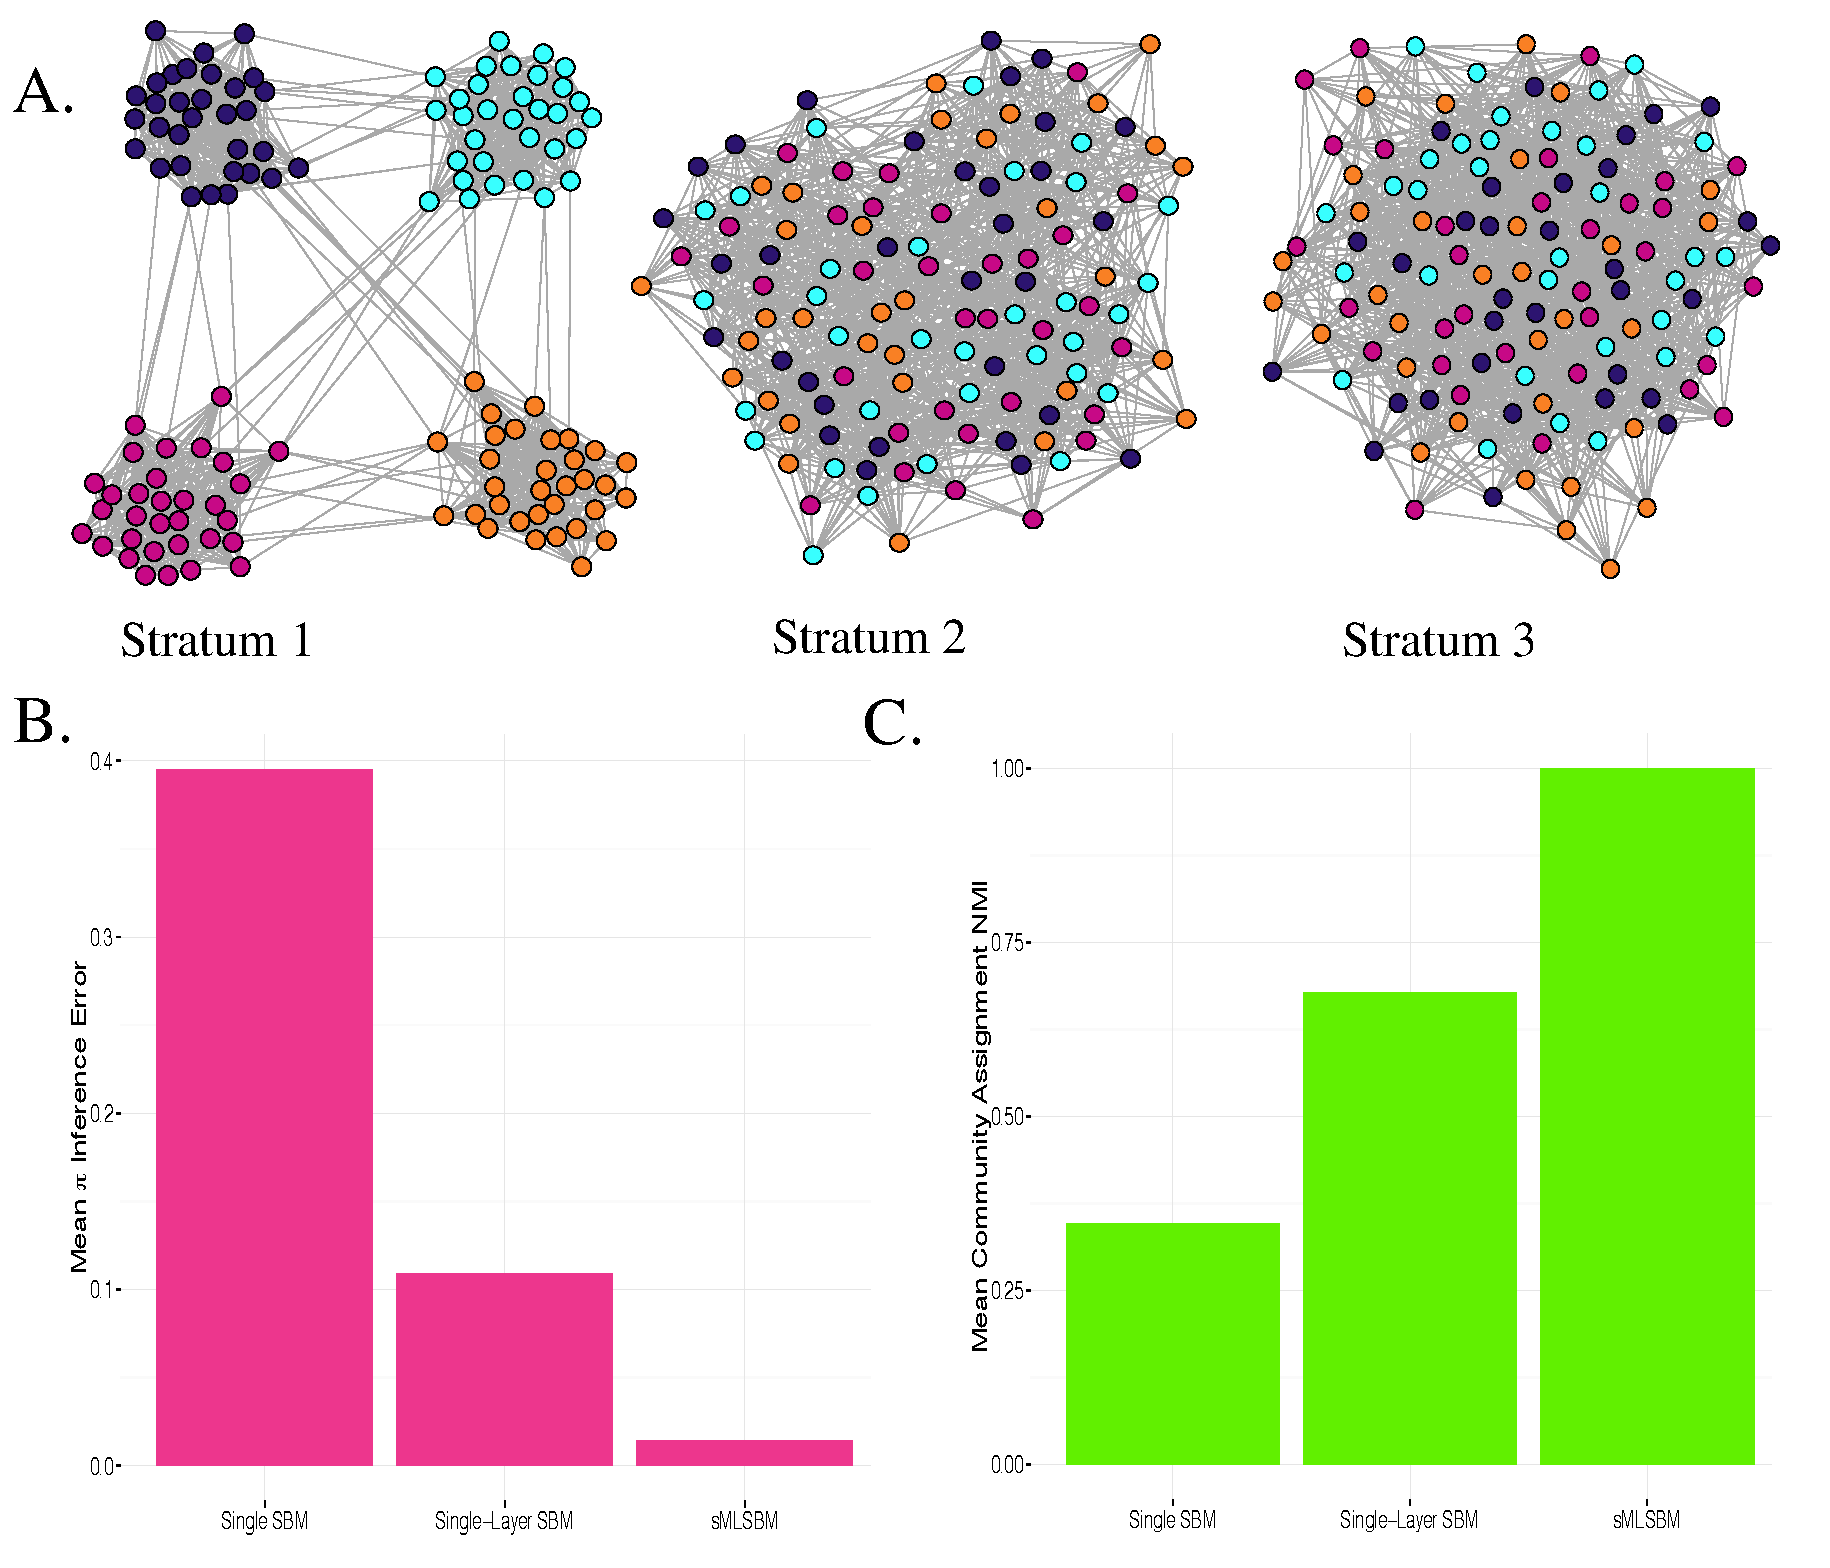
\includegraphics[width=.6\linewidth]{Figure3.pdf}
\caption{{\bf \noindent Synthetic experiment comparing sMLSBM to other SBMs.} 
%
{\bf A}.~We specified a model with $S=3$ strata and $L=10$ layers per stratum. A representative layer from each stratum is plotted. Note that nodes in all networks are colored according to their community membership in stratum 1. Each network has $N=128$ nodes, $K=4$ communities and mean degree, $c=20$. The $p_{in}^s$ parameters for $s=1,$ $2$ and 3 are 0.6, 0.4 and 0.25, respectively. Corresponding values of $p_{out}^s$ were selected to maintain the desired expected mean degree, c=20. 
%
{\bf B}. We fit 3 types of models to the 30 network layers:
i) single SBM: fitting a single SBM to all of the layers;
ii) single-Layer SBM: fitting an individual SBM to each layer; and
iii) sMLSBM: identifying strata and fitting an SBMs for each strata. 
Each model yields an estimate $\overline{{\boldsymbol \pi}^{s_l}}$ for the true SBM of each layer $l$, which is denoted ${{\boldsymbol \pi}}^{l}$. Here $s_l$ denotes the inferred strata for layer $l$.
On the vertical axis we plot the mean $\ell$2 norm error 
%between each layer's true underlying ${\boldsymbol \pi}^{l}$ and that inferred given its stratum membership $s_{l}$ under the given model. In other words, we compute, 
$||\text{vec}({\boldsymbol \pi^{l})}-\text{vec}(\overline{{\boldsymbol \pi}^{s_{l}}})||_{2}$. 
 %
 {\bf C}. For each of the three models, we computed the normalized mutual information (NMI) between the true node-to-community assignments ${{\bf z}^{l}}$ and the inferred values $\overline{{\bf z}^{s_l}}$.}
 
\end{center}
\end{figure} 

%\\\indent 
In order to compare the accuracy of fit for the three models---single-layer SBM, single SBM and sMLSBM---we quantify the inference accuracy of the SBM parameters, $\overline{{\boldsymbol \pi}^{y_{l}}}$, and community assignments, $\overline{{\bf Z}^{s_{l}}}$. 
%
First, for each layer and each model, we quantified the error ($\ell^{2}$ norm) between $\text{vec}(\overline{{\boldsymbol \pi}^{y_{l}}})$ and its true value, $\text{vec}({\boldsymbol \pi}^{l})$. Note that $\text{vec}({\bf X})$ is the $\frac{K(K+1)}{2}$ length vector representing the lower triangle of the matrix ${\bf X}$.  Moreover, to quantify error,
% parameter and the \drt{inferred parameter} $\overline{{\boldsymbol \pi}^{s_{l}}}$ under each of the \drt{three models.} 
%In other words, for each layer $l$ 
we compute $||\mbox{vec}({\boldsymbol \pi^{l}})-\text{vec}(\overline{{\boldsymbol \pi}^{s_{l}}})||_{2}$.  We note that this error is well-defined because we identify $K=4$ communities for all layers and all models. The mean error across layers under each model are shown in Fig.~3(B). In this example, sMLSBM outperforms the two other models.
%
Second, we computed for each layer the mean normalized mutual information (NMI) \cite{commdeccompare} between the true node-to-community assignments, ${\bf z}^{l}$, and the inferred values, $\overline{{\bf z}^{y_{l}}}$, under each model. In other words, for each layer, we compute, $\text{NMI}({\bf z}^{l},\overline{{\bf z}^{y_{l}}})$. Figure 3(C) shows the mean NMI for community assignments across layers. Indeed, the effects of fitting an incorrect model to a collection of layers in terms of ability to effectively estimate SBM parameters and community assignments is apparent. In particular, fitting a single SBM model results in both larger mean inference and community assignment error, compared to fitting single-layer SBMs and 3 strata sMLSBM. In other words, sMLSBM provides an efficient clustering into strata only when the layers are indeed related (i.e. generated from the same SBM), otherwise each layer is a stratum on its own.

\subsection{Synthetic Experiment with Two Strata}\label{sec:2strata}

Next, we further explored the performance of our algorithm (see Sec.~\ref{sec:Algorithm}) for inferring an sMLSBM under various situations: 1) in comparison to baseline clustering methods; 2) in response to an increase in the number of layers; and 3) under variations in levels of detectability. Specifically, we designed synthetic experiments in which we generated multilayer networks with either $L=10$ or $L=100$ layers. Every multilayer network contained $S=2$ strata (each having $K^1=K^2=4$ communities), and in each layer there were $N=128$ nodes (each having an expected mean degree of $c=16$). Note that in this example both strata have the same node-to-community assignments. The strata were fixed to be the same size, $L^1=L^2=L/2$. Similar to the experiment described in Sec.~\ref{sec:SBM1}, the SBM parameters were constructed using $p_{in}^s$ and $p_{out}^s$. Since we have already specified the expected mean degree, these parameters must satisfy the constraint $c=N(p_{in}^s+p_{out}^s)/2$ for both strata.
%
In all simulations, we fixed the SBM parameters of the first strata as $(p_{in}^1,p_{out}^1)=(.1836,.1055)$. It is also convenient to define the quantity, $N(p_{{in}}^{1}-p_{{out}}^{1})=10$, which relates to the detectability of communities \cite{decelle2011inference}. For example, the ability to detect community structure in a given layer and/or strata is, in general, expected to improve with increasing $N(p_{{in}}^{s}-p_{{out}}^{s})$. For the second strata, we allow $N(p_{{in}}^{2}-p_{{out}}^{2})$ to vary.


We present results for this experiment in Fig.~4, wherein the left and right columns give results for $L=10$ and $L=100$, respectively.

Symbols in each plot represent the mean over 50 multilayer networks, and error bars show standard error. In each plot, the vertical dotted line indicates $N(p_{{in}}^{2}-p_{{out}}^{2})=10$, which represents the point where the two strata are indistinguishable since $(p_{in}^1,p_{out}^1)=(p_{in}^2,p_{out}^2)$.
%
In Fig.~4(A), we show the NMI between the true layer-to-strata assignments and those inferred by sMLSBM, or $\text{NMI}({\bf y},\hat{\bf y})$. As a baseline, we compare sMSLBM results to directly clustering the layers' adjacency matrices using the $k$-means algorithm with $K=2$. We consistently observe higher NMI as a result of sMLSBM compared to $k$-means. More interestingly is the case with $L=100$, where both $k$-means and sMLSBM perform at least moderately well at partitioning layers into strata before the point where the strata are indistinguishable. %At this point, where the $p_{in}$ and $p_{out}$ parameters for strata 1 and 2 are the same, strata are clearly not distinguishable and we see this reflected in the drop of NMI. \\
%
In Fig.~4(B), we plot the number of iterations (NOI) required for Phase II of our algorithm to converge. We observe that as the number of layers in the network increases, so does the number of required sMLSBM iterations. Moreover, the peaks in panel B. correspond to the sudden jumps in strata NMI. 

%In both cases of $L=10$ and $L=100$, we notice a spike around when $N(p_{in}^{2}-p_{out}^{2})=20$.
%
Finally, in Fig.~4(C) we show the quality of node-to-community assignments 
%in \drt{the} strata. Particularly, we compute 
by plotting the NMI between the true and inferred node-to-community assignments as described in Sec.~\ref{sec:SBM1}. Note that stratum 1 here represents the stratum where the majority of layers were generated from model $S^{1}$ and analogously for stratum 2. Therefore, when the strata NMI is low (panel A.), we see poorer community detection results than expected, as layers get incorrectly mixed. As the strata NMI increases, layers from the same model are assigned together and the communities NMI stabilizes. 
%Specifically, we plot the mean NMI across stratum 1 (red symbols) and stratum 2 (blue symbols). As expected, we observe a general increase in NMI as $N(p_{{in}}^{2}-p_{{out}}^{2})$ increases. 
Finally, by comparing the results for $L=100$ to those for $L=10$, we observe an increase in number of layers, $L$, generally leads to an improvement in community detection and strata identification.\\


%%%%%Begin so new%%%%%%%%%%%%
\begin{figure}
\begin{center}
%\includegraphics[width=1\linewidth]{Shit}
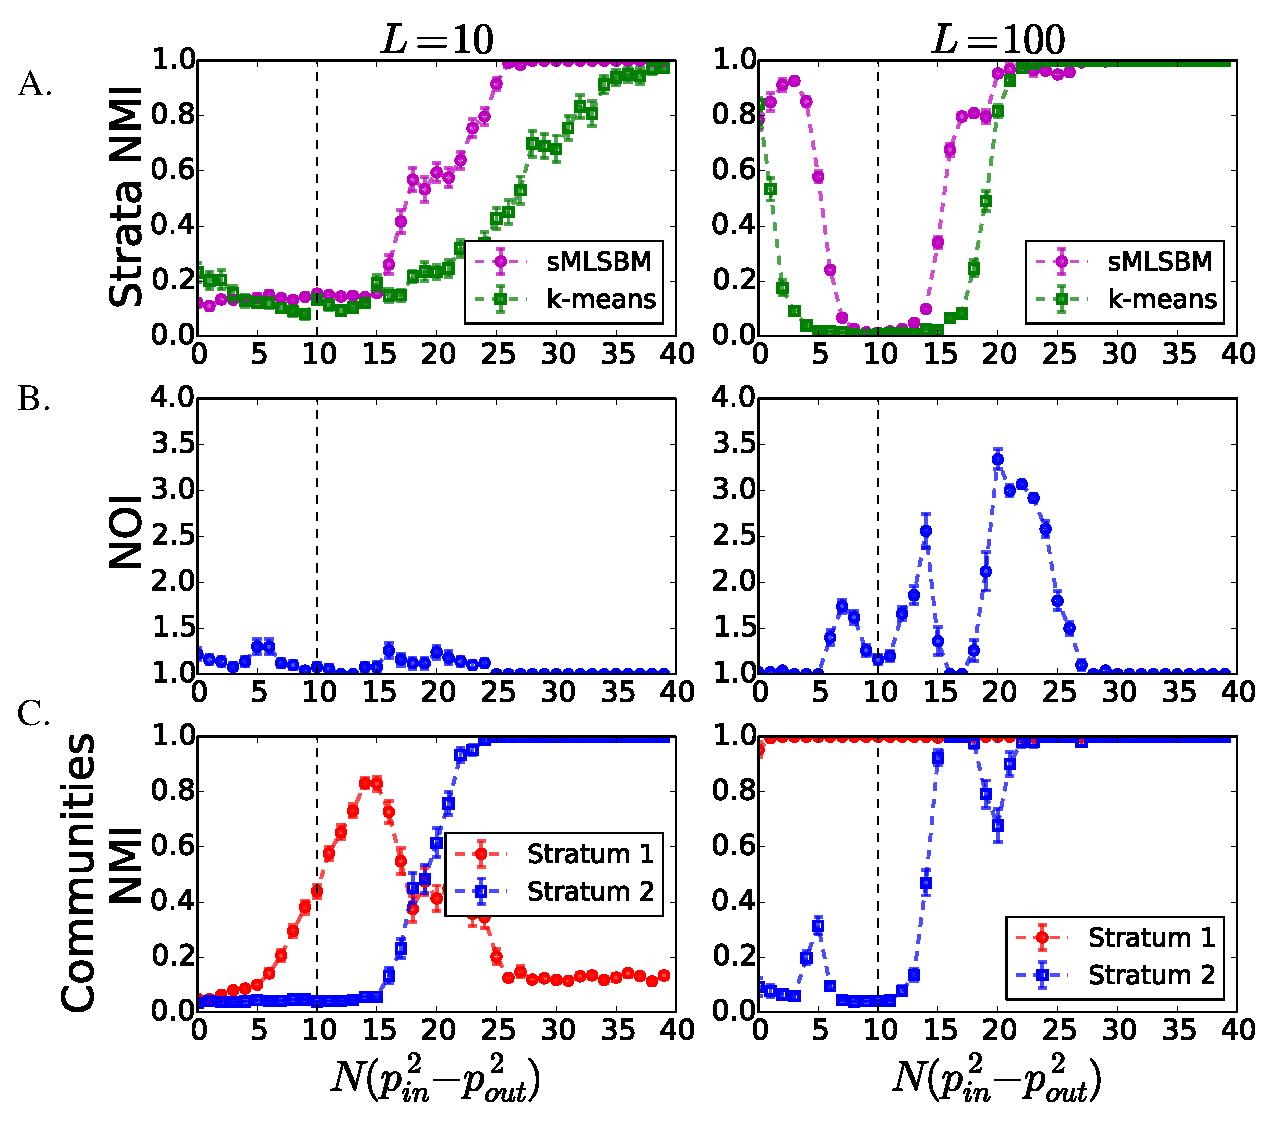
\includegraphics[width=.5\linewidth]{Figure4.pdf}
\label{fig:saray}
\caption{
{\bf Synthetic experiment with two strata.} We conducted numerical experiments with multilayer networks with $N=128$ nodes, mean degree $c=16$, $S=2$ strata and $K^1=K^2=4$ communities. The networks contained either $L=10$ (left column) or $L=100$ layers (right column), which were divided equally into the two strata. For stratum 1, we fixed the quantity $N(p_{{in}}^{1}-p_{{out}}^{1})=10$, which fully specifies $(p_{{in}}^{1},p_{{out}}^{1})$ since setting $c=16$ also constrains these parameters. In contrast, we vary $N(p_{{in}}^{2}-p_{{out}}^{2})$.
%
%Then, in each experiment we simulate 50 2- stratum networks, where the $p_{in}$ and $p_{out}$ are fixed in stratum 1, but networks in stratum 2 are generated according to $\text{Diff}_{2}$ (horizontal axis). In each plot, error bars show standard error and curves are the mean from 50 simulated networks. The vertical line in the plots shows the point at which $\text{Diff}_{1}=\text{Diff}_{2}=10$. 
{\bf A}. As a function of $N(p_{{in}}^{2}-p_{{out}}^{2})$, we plot the mean NMI to interpret the ability of sMLSBM to recover the true layer-to-strata assignments. We compare the performance of sMLSBM (purple curve) to generic $k$-means clustering (green symbols) of adjacency matrices. 
{\bf B.} We plot the mean number of iterations (NOI) required for Phase II of our algorithm to converge.
{\bf C.} Finally, we measure the quality of node-to-community assignment results by plotting the mean NMI between the true node-to-community assignments and those inferred with sMLSBM in stratum 1 (red symbols) and stratum 2 (blue symbols).}

\end{center}
\end{figure}

\section{Human Microbiome Project Example}
\indent As an application of sMLSBM, we consider correlation networks constructed from data from the Human Microbiome Project \cite{microbiome}. For various sites on the body, the human microbiome project has successfully collected multiple human samples in order to better understand interactions between bacterial species. In this context, network inference is particularly interesting, as such methods aim to capture the relationships between various organisms. Microorganisms exhibit intricate ecologies within the gut of their human host and particular body sites have been shown to possess characteristic interactions. Further, certain interactions between microbes can often be associated with particular health and disease states \cite{microbeco}. Microbiome data is typically collected through metagenomic sequencing and reads are further binned into groups, known as operational taxonomic units (OTUs), to represent particular organisms. The nature of this count-based sequencing data makes network inference challenging, and is thus an interesting field in itself. To demonstrate the potential use for sMLSBM in the context of the human microbiome, we applied our algorithm for learning sMLSBMs to multilayer networks constructed from the SparCC \cite{sparcc} network inference method. \\
\indent SparCC is a correlation network inference method that aims to approximate the linear Pearson correlation between components in a system. This method performs favorably, as it accounts for the extent of diversity in the microbial community, which plays a significant role in detecting valid interactions. Furthermore, networks are constructed with the assumptions that the number of components in the system (e.g. OTUs) is large and that the correlation network should be sparse.  As supplemental data in Ref.~\cite{sparcc}, the authors provided their inferred microbial interaction networks for 18 sites in the human body, using the sparse, SparCC framework. The edges in these networks have positive and negative real-valued weights, based on the results of SparCC inference. In this analysis, we converted the SparCC networks into binary adjacency matrices by allowing a link only if the SparCC edge-weight between two OTUs was at least 0.15 (chosen as a value close to 0.2, given in Ref \cite{sparcc}). To convert the 18 single-layer networks corresponding to species interactions in 18 body sites, we identified the collection of nodes (OTUs) that participated in at least two layers in terms of having at least one connecting edge weight value in the layer above the 0.15 threshold}. This resulted in $N=213$ unique OTUs (nodes) for our multilayer network analysis. We emphasize that restricting attention to nodes that participate in multiple layers was a choice we made in our focus on identifying common community structures across layers, to demonstrate the accuracy in the algorithm and inference procedures of sMLSBM. A more biologically-relevant treatment of this dataset should of course consider domain-specific expertise in formulating a network representation appropriate to the question at hand.\\
\indent We inferred an sMLSBM for the multilayer network and chose to show results for $S=6$ strata. That is, this selection leads us to find 6 clusters of body sites such that the microbiomes are similar between sites in the same cluster but differ from microbiomes at sites in the remaining clusters.
 We indicate these 6 strata with colored boxes in  Fig.~5. We note that due to the stochasticity of k-means in our algorithm, the communities and strata fit by sMLSBM can vary from one realization to the next. The shown strata assignments reflect those observed to yield the highest log-likelihood.

\subsection{Comparison of sMLSBM to multilayer network reducibility}
To gauge the performance of our method, we compared our strata membership results to the hierarchy obtained as part of the reducibility method developed in \cite{domen}. To do this, we followed the following steps: 
\begin{enumerate}
\item Compute the normalized Laplacian matrices for each of the 18 body site networks;
\item Compute the eigenvalues for each normalized Laplacian matrix;
\item Use these eigenvalues to compute the Von Neumann entropies for individual layers and pairs of layers;
\item Use the Von Neumann entropies to compute Jensen-Shannon distances between pairs of networks; and
\item Perform hierarchical clustering using the Jensen-Shannon distances and Ward linkage. 
\end{enumerate}
We show the results of this hierarchical clustering with a dendrogram in Fig.~5, which are 
%
%The dendrogram resulting from this sequence of steps produces a grouping that is relatively faithful to body regions in terms of groups of body sites that are spatially proximal. To visualize the comparison between sMLSBM results and this hierarchical tree, we designate members of each stratum with different colored boxes around the corresponding leaves. 
in very good agreement with the sMLSBM results. However, as expected, we observe slight differences, since these methods cluster layers based on different criteria; in particular, sMLSBM partitioning reflects similarity only in community structure. \\
%
\indent The results of both methods are relatively faithful to body regions in terms of groups of body sites that are spatially proximal. The only exception to this observation is the brown-colored stratum in Fig.~5, which is comprised of some seemingly unrelated body sites. While this grouping may not be intuitive, there is biological evidence to explain its plausibility. Specifically, Ref.~\cite{dingcluster} offers a state-of-the-art clustering of body sites based on biological expertise. Here, the authors have advanced understanding of microbial community composition through the application of a multinomial mixture model to define community types to characterize body sites. In particular, each sample collected through the Human Microbiome Project was assigned to 1 of 4 community types. They then quantified relationships between body sites using the p-value from a Fisher exact test on the membership of samples to community types. Similar to what we observe  in the brown-colored stratum, the authors of \cite{dingcluster} found a surprising correlation between samples from stool and oral cavity, which is reflected in our result. 

\begin{figure*}[t]
\begin{center}
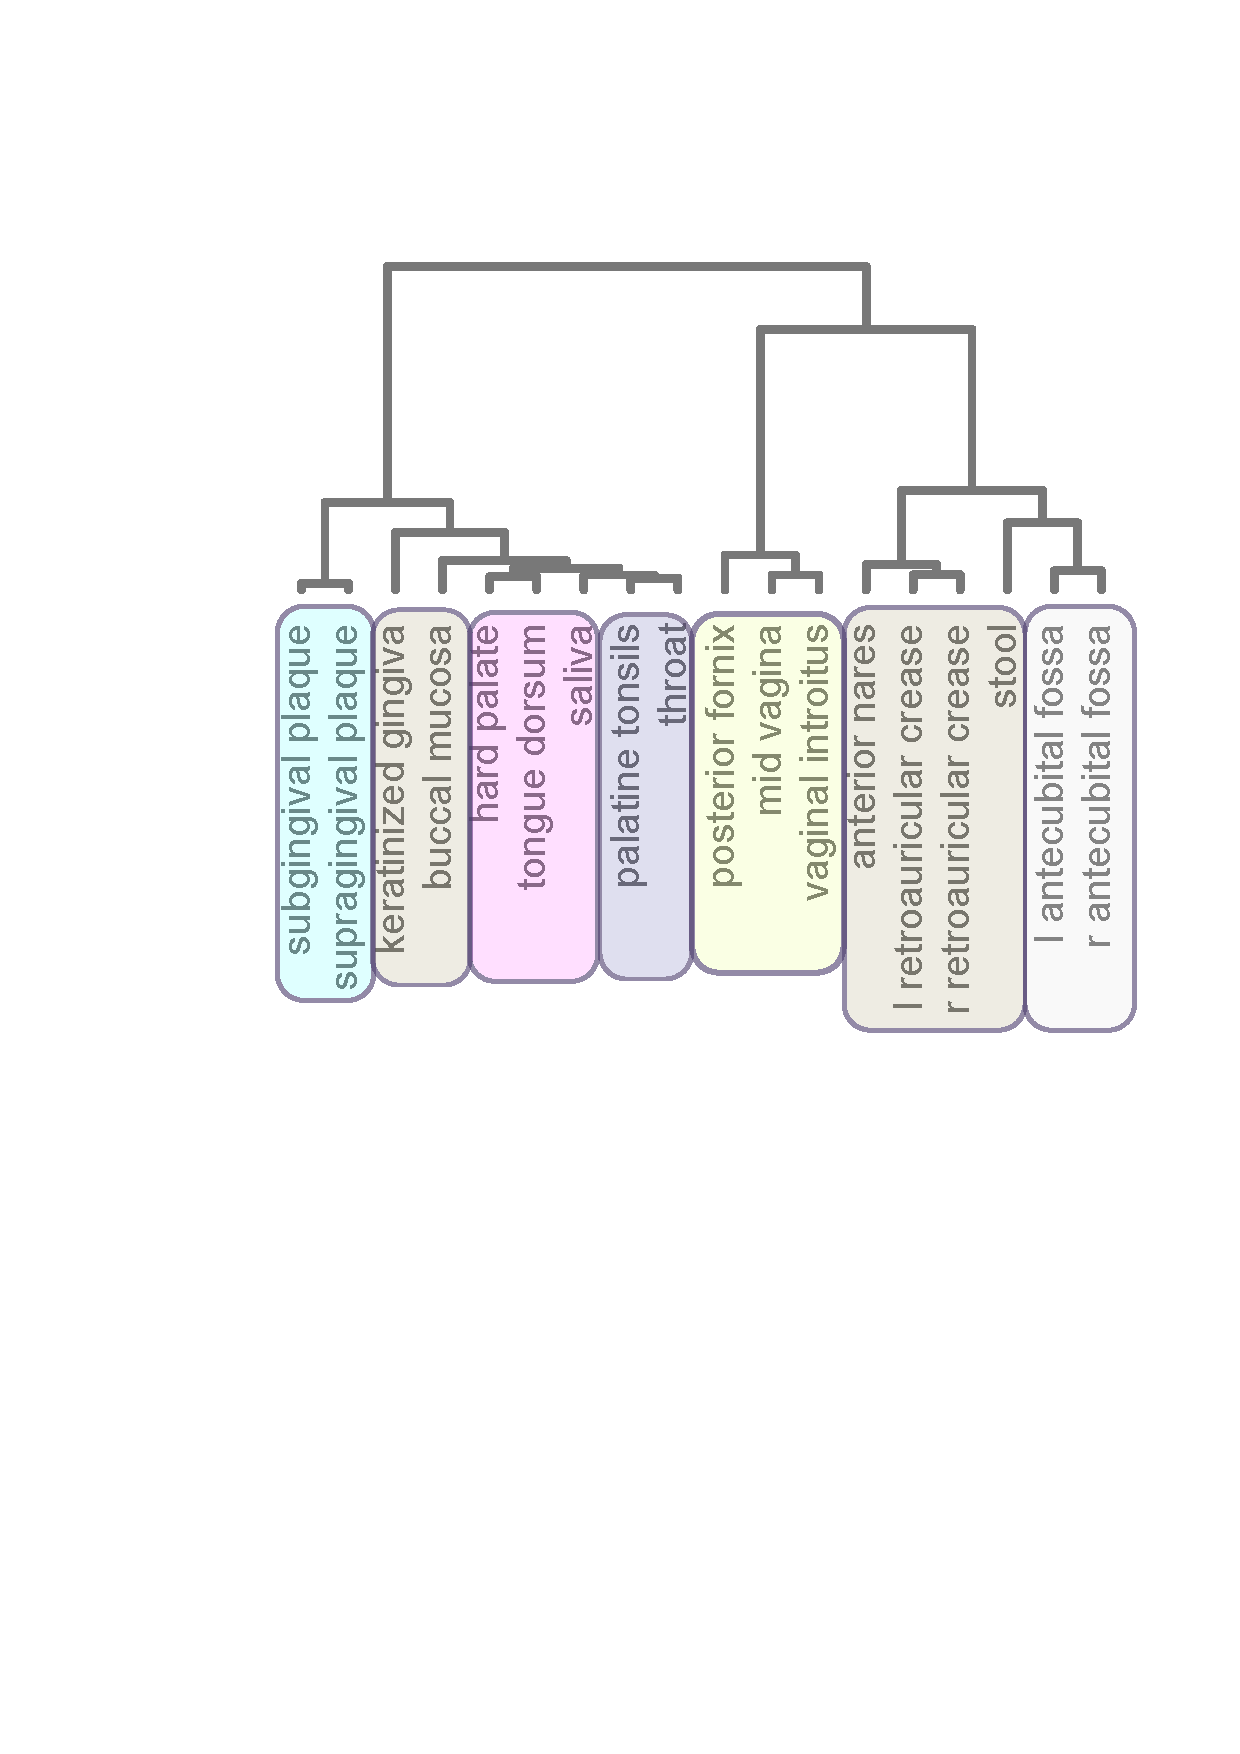
\includegraphics[width=.5\linewidth]{Fig5.pdf}
\caption{{\bf Comparison of sMLSBM on the OTU interaction networks \cite{sparcc} for each of the body sites to a reducibility hierarchy \cite{domen}.} As described in the text, we consider a multiplex network with $L=18$ layers and $N=213$ nodes, which we group here into $S=6$ strata, while the dendrogram was generated by the method employed as the precursor to the reducibility framework. Colored boxes around the leaves of the dendrogram designate the body site to strata assignments obtained with sMLSBM.}
\end{center}
\end{figure*}

\subsection{Generating samples from the fitted sMLSBM}

\indent In Fig.~6, we illustrate network layers for 4 of the 6 strata that we identify to highlight one advantage of having a probabilistic generative model for microbial composition shared in subsets of body sites. Specifically, each row provides information about the network layers and their fitted sMLSBM model for a particular stratum. Each grid in the figure represents the binary adjacency matrix encoding interactions between OTUs: a colored dot at position $(i,j)$ indicates the existence of an edge $(i,j)$ in the corresponding network layer.
%Edges, or a 1 in the adjacency matrix, are colored. 
In the first column of each row is a sample network generated with the learned SBM parameters of that stratum, $\overline{{\boldsymbol \pi}}^{s}$ and $\overline{{\bf Z}^{s}}$. Columns 2 and 3 show two representative network layers within the stratum. Note that while some strata have more than two members, for illustrative purposes we only show two example layers. 
It is easy to see the very similar block structure between all networks in a given row, corroborating the usefulness of the sMLSBM approach. Finally, we highlight the usefulness of fitting sMLSBM to this multilayer network as each stratum
 elucidates a mechanistic understanding of the relationship between groups of OTUs, which could inspire further biological understanding or inquiry. 

\begin{figure}
\begin{center}
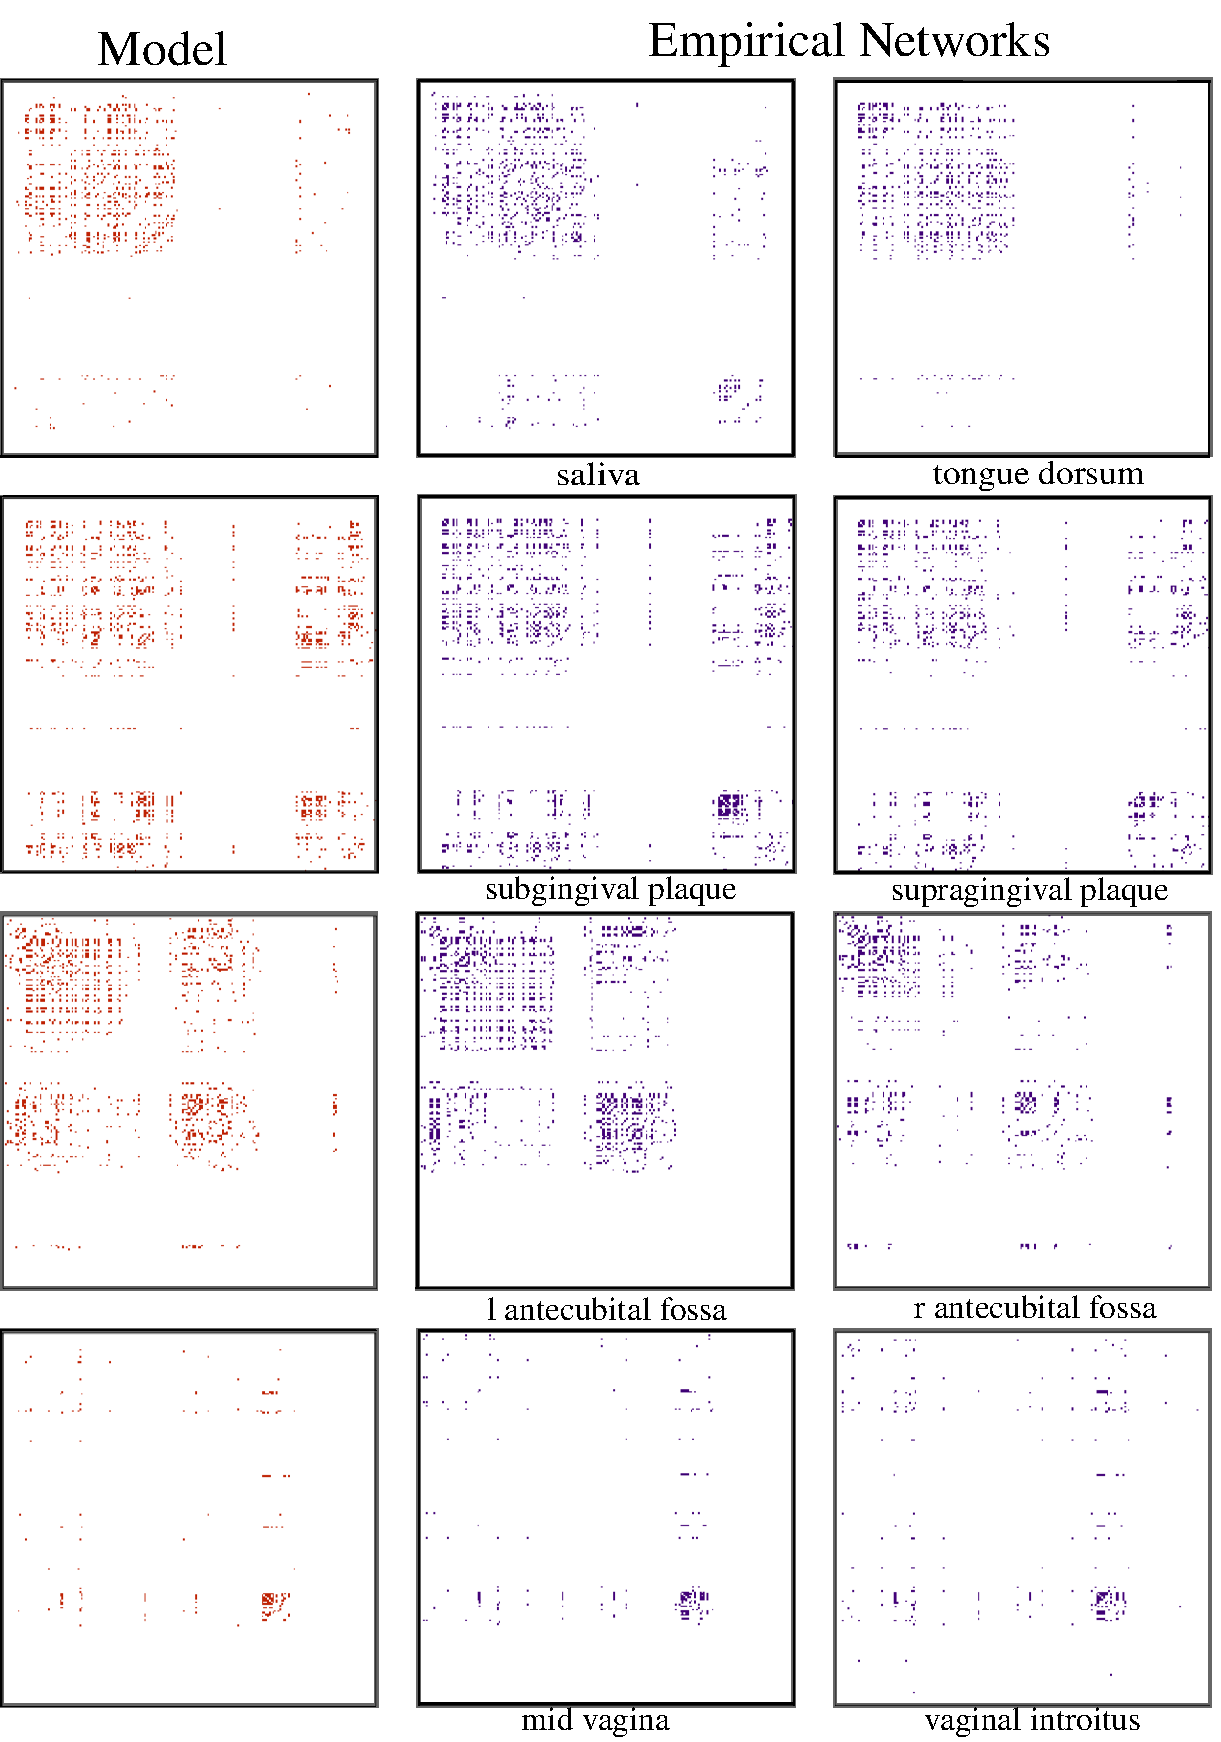
\includegraphics[width=.6\linewidth]{Fig6_Dec15.pdf}
\caption{{\bf Visualization of Strata in SparCC Networks.} We visualize the adjacency matrices for SparCC networks that encode microbiome interactions at body sites. In each panel, a colored dot at position $(i,j)$ indicates the existence of an edge $(i,j)$ in the corresponding network layer. The four rows correspond to four different strata. In column 1, we show a sample network generated from the SBM parameters, $\overline{{\boldsymbol \pi}^{s}}$ and $\overline{{\bf Z}^{s}}$, that we inferred for that stratum. In Columns 2 and 3, we show SparCC networks from that particular stratum. Note the strong similarity across each row.}
\label{sampleNet}
\end{center}
\end{figure}

\section{Concluding remarks for sMLSBM}

\indent 
We developed a novel model for multilayer stochastic block models (MLSBMs) and an associated algorithm to jointly partition layers into strata and nodes into communities. Our model assumes that layers belonging to a stratum have community structure following the same underlying SBM. To fit sMLSBM to a multilayer network, and more-specifically, a multiplex network, we iteratively alternate between rearranging layer-to-strata assignments and updating the model parameters for each stratum. Having multiple networks within a stratum---hence multiple realizations from some underlying model---helps to make inference more accurate. Particularly, more accurate assignments of nodes-to-communities within a stratum leads to improved estimation of SBM probability parameters, and vice versa. 
We have shown for multiplex networks with several strata (e.g., see Fig.~3) that inaccuracies can arise if one attempts to fit a single SBM to the network or study the network layers in isolation.
%If layers from different models were all considered to have arisen from the same SBM, both the community memberships and SBM parameters used to represent each layer would be noisier and inaccurate. 
In contrast, our model allows for an understanding of the similarities between layers in a network, in terms of their community structure. 
%
\\\indent
The ability to identify strata within collections of network layers holds promise in numerous applications. 
One motivating application is network reducibility, whereby one compresses a multilayer network by aggregating similar layers \cite{domen}. We stress that although reducibility is a closely related pursuit, it is fundamentally different from our co-clustering pursuit of simultaneously identifying communities and strata. In particular, our approach does not provide a method for aggregating layers. Instead, sMLSBM compresses the network information in the sense that the learned SBM parameters represent a consensus for each stratum, and those consensus parameters can be used to generate a representative sample network for that stratum. For applications in which layer aggregation is sought, there are a variety of ways to aggregate layers in a strata. See, for example, Ref.~\cite{taylor2015enhanced}, where the authors explore the effects on community structure for different aggregation methods. We highlight that the sMLSBM modeling approach is appropriate in situations where one seeks a generative model for community structure, and it may be particularly appropriate when application-specific evidence suggests that subsets of networks have characteristic differences in community structure.
%
\\\indent Our comparison of sMLSBM to the reducibility method of Ref.~\cite{domen} (see Fig.~5) for the application of studying microbial interaction networks reveals several extensions to sMLSBM that could make the approach more accurate and applicable to a wider range of applications. 
First, the reducibility method \cite{domen} does not require networks to be undirected and unweighted, and it could be quite useful to extend the sMLSBM framework to
%since the pairwise distance between networks used there is based on spectral properties. Extensions to 
weighted and directed networks following the extensions for single-layer SBMs, as developed in \cite{weightSBM} and \cite{sbmdirect}, respectively. 
%We note several additional} extensions to sMLSBM that could make the approach more accurate and applicable to a wider range of applications. 
It would also be useful to extend to degree-corrected and overlapping (i.e., mixed-membership) communities \cite{degreecorrectSBM}, as well as mixed membership of layers into strata.
%, could be quite useful. 
%
%
%\\\indent 
Additionally, the Human Microbiome example reveals some interesting biological questions that could facilitate the development of more advanced network tools. To construct the multilayer network, negative edges were thresholded away; however, antagonistic relationships between microbes are known to be important \cite{antagonism}. Thus, it would be useful to develop a signed version of sMLSBM that allows edges to be either positive or negative. \\
\indent The rise of a greater number of multilayer network datasets is providing the need for additional tools for the construction and analysis of such networks. The sMLSBM provides a new method to find signal in inherently noisy and complex network data. 

\section{Detectability in a single stratum}
The development of sMLSBM motivated the analysis for how multiple layers can be collectively used to more accurately learn SBM model parameters in the single stratum case. That is, given a collection of sparse networks from a multilayer stochastic block model with one stratum, how can the layers most accurately be combined to give the most accurate definition of community structure. In work lead by Dane Taylor and collaborators Saray Shai, and Peter Mucha, we investigate these questions in \emph{Enhanced detectability of community structure in multilayer networks through layer aggregation} \cite{taylor2015enhanced}. In particular, we studied the detectability limitations of the stochastic block model for a multilayer network with 1 stratum using random matrix theory techniques. 

\subsection{Investigating detectability in a multilayer network}
Community structure detectability has gained considerable attention \cite{detect20,detect21,detect22,detect23,detect24,detect25} with a hope of being able to identify properties of networks and their corresponding adjacency matrices that reveal how prominent or easy-to-find the community structure is. A network with detectable community structure is thought to be one where multiple community detection algorithms would agree on common groups, and that nodes are not just being assigned to communities randomly, but instead exhibit straight-forward clustering patterns. Applying a community detection algorithm to a network with undetectable community structure might be dramatically different between algorithms, or may assign nodes to the biggest community or even all to the same community. It is particularly interesting to investigate this question in relation to a multilayer stochastic block model because we can generate samples from various models with different parameters and see if the community partition of the network agrees with the specified model. Previous work has previously been explored in networks with degree heterogeneity \cite{detectDegreeHetero}, hierarchical structure \cite{peixotoHierarchAttribute,HierarchAttl}, and in temporal networks \cite{detectTemporal}, but not characterized in multilayer networks. \\
\indent To study this in multilayer networks, we use random matrix theory to study a multilayer network generated from a stochastic block model, and enumerate ways that these layers can be \emph{aggregated} or combined to most improve community structure. We show that the detectability limit vanishes with an increasing number of layers, $L$, and decays as $O(L^{-1/2})$ when we aggregate the the network layers, by taking the sum of their adjacency matrices. Further, we also explore the detectability limits of this aggregated summation of adjacency matrices  that are thresholded to a binary adjacency matrix according to some value, $\tilde{L}$.  

\subsection{Studying detectability in two block networks}
In this work, we study a 2 block multilayer stochastic block model. As seen in previous sections, each network layer has the same set of $N$ nodes and parameterized by an $N$-length vector, ${\bf z}$ specifying the node-to-community assignments and a $2 \times 2$ community probability connectivity matrix, ${\boldsymbol \theta}$. Further, we assume that the between probability connection probability is denoted by $p_{out}$, and that $\pi_{1,2}-\pi_{2,1}=p_{out}$. Similarly, we denote the within-community probability as $p_{in}$, so that $\pi_{1,1}-\pi_{2,2}=p_{in}$ Previous work has shown that for the large network limit, as $N \rightarrow \infty$, there is a solution to the detectability limit \cite{detect23,detect24}, characterized by the solution curve $(\Delta^{*},\rho)$ to 

\begin{equation}
\label{detectEquation}
N\Delta=\sqrt{4N\rho},
\end{equation} 

where $\Delta=p_{in}-p_{out}$ is the difference in probability and $\rho=(p_{in}+p_{out}/2$ is the mean edge probability. For a given value of $\rho$, the communities are only detectable (or correctly characterized) if $\Delta > \Delta^{*}$. Equation \ref{detectEquation} was derived for sparse networks (i.e. constant $\rho N$ so that $\rho=O(N^{-1})$) and was obtained using both a Bayesian analysis \cite{detect23} and random matrix theory \cite{detect24}.\\
\indent In this work , we study the behavior of $\Delta^{*}$ for two methods of aggregating layers within a multilayer network of $L$ layers, which we denote $\mathcal{L}$. We define the \emph{summation} network, $\bar{\bf A}=\sum_{l \in \mathcal{L}} {\bf A}^{l}$. Note that, ${\bf A}^{l}$ gives the adjacency matrix for network layer, $l$. We also define a family of \emph{thresholded} networks, with unweighted adjacency matrices $\{\hat{{\bf A}}^{\tilde{L}}\}$ that are obtained by applying a threshold $\tilde{L}=\{1, \dots, L\}$ to the entries of $\bar{\bf A}$. Under this thresholding rule, $\hat{A}_{ij}^{\tilde{L}}=1$ if $\bar{A}_{ij} \ge \tilde{L}$ and is 0 otherwise. We are particularly interested in the limiting cases when $\tilde{L}=L$ and when $\tilde{L}=1$, which correspond to applying logical AND and OR operations to the original multilayer data $\{A_{ij}\}$, for a fixed pair of nodes $(i,j)$. We refer to these thresholded networks as the AND and OR networks, respectively. 

\subsection{Using random matrix theory to study detectability}
\indent Since node-to-community assignments, ${\bf z}$ can be inferred with spectral method, random matrix theory \cite{detect38,detect39} is a useful approach for studying partitioning and phase transitions in detectability (i.e. node-to-community assignment accuracy) \cite{detect24,peixotoHierarchAttribute,HierarchAttl}. Using this approach, phase transition in detectability correspond to the disappearance of  gaps between eigenvalues (whose corresponding eigenvectors reflect community structure) and bulk eigenvalues [which arise due to stochasticity and whose $N \rightarrow \infty$ limiting distribution is given by a spectral density $P(\lambda)$. The theory we develop in this work is based on the modularity matrix, $\bar{B_{ij}}=\bar{A}_{ij}-\rho L$ \cite{newmangirvan}. \\
\indent We first study $\Delta^{*}$ for the summation network. We analyze the distribution of real eigenvalues $\{\lambda_{i}\}$ of ${\bf \bar{B}}$ (in descending order). First, we describe the statistical properties of entries $\{\bar{A_{ij}}\}$, which are independent random variables following a binomial distribution with $P(\bar{A_{ij}}=A)=f(a;L,\pi_{z_{i},z_{j}})$, where

\begin{equation}
f(a;L,p)={L \choose a}p^{a}(1-p)^{L-a}
\end{equation}

has mean $Lp$ and variance $Lp(1-p)$. With sufficiently large variance in the edge probabilities, we find that the limiting $N\rightarrow \infty$ distribution of bulk eigenvalues for ${\bf \bar{B}}$ is given by a semicircle distribution,

\begin{equation}
P(\lambda)=\frac{\sqrt{\lambda^2_{2}-\lambda^{2}}}{\pi \lambda_{2}^{2}/2}
\end{equation}

The largest eigenvalue of $\bar{{\bf B}}$ in the $N \rightarrow \infty$ limit is the isolated eigenvalue,

\begin{equation}
\lambda_{1}=NL\Delta/2+2[\rho(1-\rho)-\Delta^{2}/4]/\Delta. 
\end{equation}

The eigenvector ${\bf v}$ corresponding to $\lambda_{1}$ gives the spectral bipartition. Here, the inferred community label of node $i$ is determined by the sign of $v_{i}$ and provided that the largest eigenvalue corresponds to this isolated eigenvalue, $\lambda_{1}$, the eigenvector entries $\{v_{1}\}$ are correlated with the node-to-community labels, ${\bf z}$.  As shown in \cite{taylor2015enhanced}, we can derive a detectability equation that accounts for the number of layers,

\begin{equation}
NL\Delta=\sqrt{4NL\rho(1-\rho)}.
\end{equation}

\indent We now study $\Delta^{*}$ for the thresholded networks, which correspond to single-layer SBMs in which the community labels, ${\bf z}$ are identical to those of the multilayer SBM, but are new effective block edge probabilities

\begin{equation}
\hat{\Pi}_{nm}^{(\tilde{L})}=1-F(\tilde{L}-1;L,\Pi_{nm}),
\end{equation}

where $F(a;L,p)$ is the cumulative distribution function for the binomial distribution $f(a;L,p)$. The effective probabilities for the AND and OR networks are $\hat{\Pi}_{nm}^{(L)}=(\Pi_{nm})^{L}$ and $\hat{\Pi}_{nm}^{(1)}=1-(1-\Pi_{nm})^{L}$, respectively. For the two-community SBM, the effective probabilities are $\hat{p}_{\text{in,out}}^{(\tilde{L})}=1-F(\tilde{L}-1;L,p_{\text{in,out}})$, $\hat{\Delta}^{(\tilde{L})}=\hat{p_{in}}^{(\tilde{L})}-\hat{p_{in}}^{(\tilde{L})}$ and $\hat{\rho}^{(\tilde{L})}=\hat{p_{in}}^{(\tilde{L})}-\hat{p_{in}}^{(\tilde{L})}/2$. 


\subsection{Results}

In Figures \ref{Detect} (a) and (b), we show $\Delta^{*}$ versus the mean edge probability, $\rho$ for the different aggregation methods: (i) a single layer (red dot-dashed curves), which is identical in panels (a) and (b); (ii) the summation network (blue dashed curves), for which the curve in (b) corresponds to the curve in panel (a) rescaled by a factor of 1/2; and (iii) thresholded networks (solid curves), which shift left-to-right with increasing $\tilde{L}$. This is evident by comparing $\Delta^{*}$ for the AND ($\tilde{L}=L$, gold circles) and OR $\tilde{L}=L$, cyan squares) networks. We find that when $\rho$ is large that the AND (OR) network has a relatively large (small) detectability limit. In other words, aggregating layers using the AND (OR) operation is beneficial for dense (sparse) networks. Note that the results shown in Figure \ref{Detect} are just a subset of results from Taylor \emph{et al.,} \cite{taylor2015enhanced}. 

\begin{figure}
\begin{center}
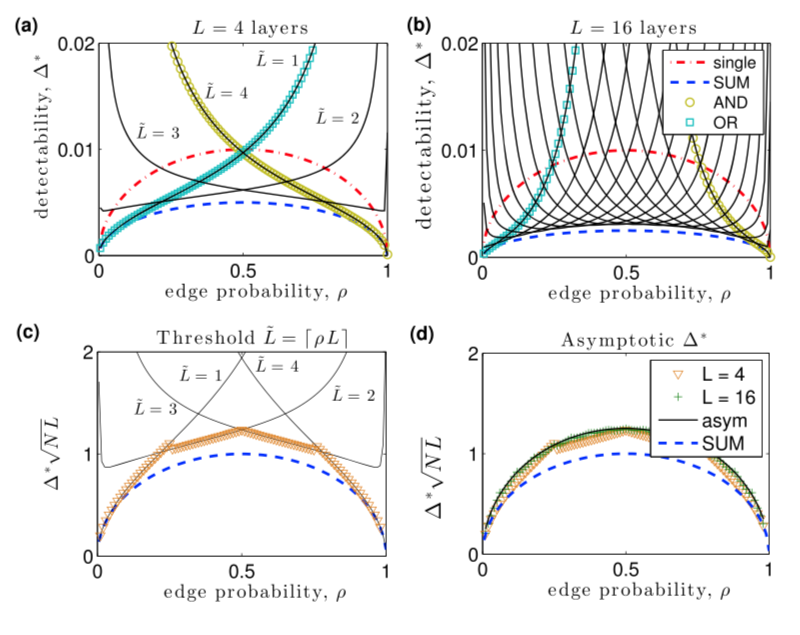
\includegraphics[width=.6\linewidth]{Detect}
\caption{{\bf Effects of layer aggregation on detectability.} Layer aggregation enhances the detectability of community structure. (a),(b). We plot the detectability limit $\Delta^{*}$ versus mean edge probability $\rho$ for a single network layer (red dot-dashed curves), the aggregate network obtained by summation (blue dashed curves), and aggregate networks obtained by thresholding this summation at $\tilde{L} \in \{1,2,3,4\}$ (solid curves). Gold circles and cyan squares highlight $\tilde{L}=L$ and $\tilde{L}=1$, which we refer to as AND and OR networks, respectively. Results are shown for $N=10^{4}$ nodes with (a) $L=4$ and (b) $L=16$ layers. (c) For $L=4$, we show $\Delta^{*}$ versus $\rho$ for the optimal threshold $\tilde{L}=\ceil*{\rho L}$ (orange triangles), which lies on the solution curves for $\tilde{L} \in \{1,\dots,L\}$ (solid curves). (d) We show $\Delta^{*}$ for $\tilde{L}=\ceil*{\rho L}$ with $L \in \{4,16\}$. These piecewise-continuous solutions collapse onto the asymptotic solution $\delta_{\text{asym}}^{*}$ (black curve) as $L$ increases. In panels (c), (d), we additionally plot $\delta^{*}$ for the summation network (blue dashed curves). }
\label{Detect}
\end{center}
\end{figure}

\subsection{Conclusion}

In this work, we studied limitations on community detection for multilayer networks with layers drawn from a common SBM. As an illustrative model, we analyzed the effect of layer aggregation on the detectability limit $\Delta^{*}$ for two equal-sized communities. When layers are aggregated by summation, we analytically showed that $\Delta^{*}$ vanishes as $O(L^{-1/2})$. When layers are aggregated by thresholding this summation, $\Delta^{*}$ depends on the choice of threshold, $\tilde{L}$. For $\tilde{L}=\ceil*{\rho L}$, we analytically found $\Delta^{*}$ to also vanish as $O(L^{-1/2})$. We note that our analysis also describes layer aggregation by taking the mean, $L^{-1}\sum_{l}{\bf A}^{(l)}$, since the multiplication of a matrix by a constant simply scales the eigenvalues by that constant. Thus, our results are in agreement with previous work that proved the consistency of spectral clustering via the mean adjacency matrix \cite{airoldi}. \\
\indent Finally, it is commonplace to threshold pairwise-interaction data to construct network representations that are sparse and unweighted and can be studied at a lower computational cost. Our research provides insight into this common-yet not well understood-practice. It would be interesting to extend this work to allow the SBMs of layers to be correlated \cite{detect25} (that is, rather than identical) or organized into `strata' \cite{smlsbm} (i.e., layers within a single stratum are similar, but they differ across strata). We are currently extending our analysis to hierarchical stochastic block models. 

\chapter{Network compression for community detection with super nodes}
\indent In practice, social and biological networks are quite large with hundreds of thousands or millions of nodes. For example, the SNAP (Stanford Network Analysis Project) network repository (\cite{https://snap.stanford.edu/data/}) houses various types of social and technological networks. For example, the amazon co-purchasing network has 548,000 nodes and 1,788,725 edges. Working with a network this size is overwhelming and makes computations slow and variable. In particular, we will show that community detection algorithms produce highly variable outputs on large networks or take a long time to run. In this chapter, we will introduce a pre-processing technique for networks to take the originally large network and reduce it to a smaller size, which enables analysis on a small network with a user-defined number of nodes or `super nodes'. This work is from our paper \emph{Compressing Networks with Super Nodes} \cite{compressing}.

\section{Super pixel pre-processing of images}
Much of our motivation for this network pre-processing step for community detection is inspired by the image analysis literature. The identification of communities in networks is in some ways similar to multi-label image segmentation, which aims to partition a grid of pixels into contiguous regions corresponding to objects in the image. In this sense, each segmented region can be viewed as a community \cite{browet}. To speed up segmentation for large images, a popular approach is to avoid computing segmentations at the pixel level and instead reformulate the segmentation problem based on larger-scale image primitives that are likely part of the same partition. Specifically, this can be accomplished by {\it super pixels} that aggregate pixels together in a way that faithfully adheres to image boundaries, maintaining or improving segmentation accuracy \cite{slic}. The SLIC super pixel method \cite{slic} chooses seed pixels across the image's pixel grid to serve as the super pixel centers and then iteratively grows out and recomputes based on aggregation with neighboring pixels with similar visual features. This is shown in Figure \ref{fig:superPix}, where if our task is to separate the grass from the dog, the input to the segmentation algorithm would be a $1147 \times 1147$ grid of pixels (left image). By representing the image with 600 super pixels (right image), we instead use this 600 super pixel representation as the input to a segmentation algorithm, which performs segmentation by partitioning the super pixels. From this segmentation on the super pixel representation, the labels can be mapped onto the full $1147 \times 1147$ image grid based on their super pixel assignment. We seek to perform the analogous task on networks, which is pre-processing the network into `super nodes' before applying the community detection algorithm. Similar to a quality super pixel representation, we would like our super node representation to adhere to boundaries and produce accurate results. In this case, we refer to boundaries as communities that would have been obtained using the full network. Similarly, we gauge accuracy based on how similar the result obtained on the super node representation is to that on the full network. This task is more straightforward on an image because it is simply a grid of pixels, so it is easy to account for the spatial information, or the idea that neighboring pixels should be agglomerated into the same super pixel. 

\begin{figure}
\begin{center}
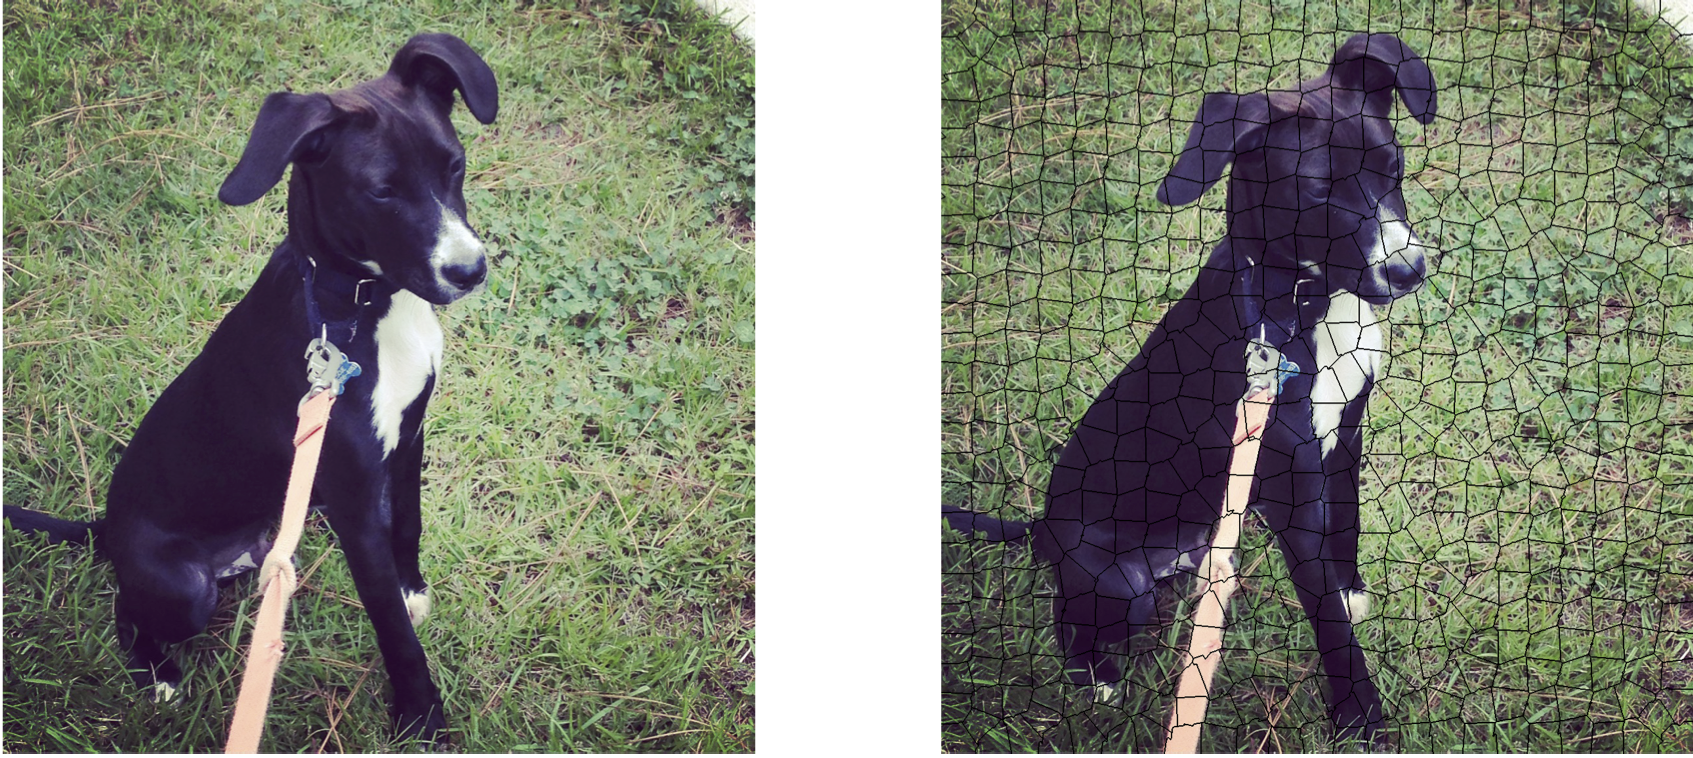
\includegraphics[width=.6\linewidth]{hamilton.png}
\caption{{\bf Superpixel pre-processing of an image.} An image can be represented by a $1147 \times 1147$ grid of pixels (left). Representing the image with 600 super pixels (right), reduces the size of the image and hence the segmentation problem is to partition the set of 600 super pixels. }
\label{fig:superPix}
\end{center}
\end{figure}

\section{Super node pre-processing for networks}
In this work, we seek to extend the super pixel methodology to large networks. In doing so, we designed experiments and validation metrics to measure the quality of our results. In images, there is a natural notion of a ground truth segmentation that can be specified by a human. Because community detection is an inherently unsupervised analysis, we had to think carefully about quantities that we could compute to measure the quality of a super node representation.

\subsection{Problem Formulation}
For a network with $N$ nodes that we will split into $K$ communities, we seek to find a representation of the network with $S$ super nodes optimizing the following two quantities. First, given the set ${\bf s}=\{s_{1},s_{2},\dots s_{S}\}$ of $S$ super nodes and $K$ communities, ${\bf k}=\{k_{1},k_{2}, \dots k_{K}\}$ identified with the full network, we wish to minimize the under segmentation error, 
\begin{equation}
\label{UnderSeg}
U=\frac{1}{K}\sum_{k_{i}=1:K}\frac{[\sum_{s_{j}|s_{j}\cap k_{i}\ne \emptyset}|s_{j}|]-|k_{i}|}{|k_{i}|}\,,
\end{equation}
where $|\cdot|$ represents the count or number of nodes in the indicated set.

We let ${\bf z}^{\text{Full}}$ and ${\bf z}^{\text{SN}}$ denote the node-to-community assignments for the full network and super node network representations, respectively. To compute the similarity between ${\bf z}^{\text{Full}}$ and ${\bf z}^{\text{SN}}$, we use Normalized Mutual Information (NMI).\cite{danon} That is, for partitions ${\bf z}^{\text{Full}}$ and ${\bf z}^{\text{SN}}$ with $p$ and $q$ communities, respectively, with $N$ the $R \times C$ contingency table matrix where $N_{ij}$ gives the count of the number of shared nodes in community $i$ in  ${\bf z}^{\text{Full}}$ and community $j$ in ${\bf z}^{\text{SN}}$, the NMI between the two partitions is 
\begin{equation}
\label{NMI}
\small{\text{NMI}({\bf{z}}^{Full},{\bf{z}}^{SN})=\frac{-2\sum\limits_{i}\sum\limits_{j}N_{ij}\log \frac{N_{ij}N}{N_{i.}N_{j.}}}{\sum\limits_{i}N_{i.}\log\frac{N_{i.}}{N}+\sum\limits_{j}N_{.j}\log\frac{N_{.j}}{N}}}\,,
\end{equation}
where $N_{i.}$ and $N_{.j}$ are the marginal sums over the corresponding rows and columns and $N=\sum_i N_{i.}=\sum_j N_{.j}=\sum_{ij} N_{ij}$. 

\subsection{An opportunity for super nodes in community detection}
While there are a variety of approaches to identify communities, in this paper we specifically examine how the compressed version of a network can be used in modularity maximization and likelihood maximization (through a stochastic block model)
 These agglomerative heuristics for both modularity and likelihood maximization simplify a computationally challenging task but can still be time consuming for large networks and often give rise to large variability in the partitions returned across multiple runs of the algorithms. We seek to explore how a compressed network representation can improve these issues. Motivated by how this problem is approached for super pixels in images, we wish to define seed nodes in networks that can be used as a starting point to grow out `super nodes' to define a new, smaller network upon which we apply standard community detection algorithms. Creating a direct analog of super pixels in networks is challenging because the inherent geometry of a network can be quite different from the grid layout of an image (where simple neighborhood structures such as 4- or 8-neighborhoods are typically used), and we need to ensure seeds are well distributed across the network. Further, while super pixels are largely constrained by the structure of the pixel grid (i.e. proximity between pixel pairs matter), their definition also incorporates extra image features to refine members of a super pixel set, whereas in network community detection we typically only have the edges of the network to work with. Finally, the performance of a super pixel representation of an image can be objectively validated from the quality of the corresponding segmentation result, with reference to human-specified objects in images; in contrast, community detection is typically an unsupervised, exploratory data analysis technique with limited available notions of `ground truth' \cite{jureTruth}. As such, we must develop measures that can be used to validate the quality of the super node representation.
 
 \section{Background}
 \subsection{Related Work}
 Our objective to define a smaller network of super nodes is a form of network compression. Several references have explored useful ways to compress networks,\cite{supergenomic,SuperNodeSide,gilbert,peng} with Yang \emph{at al.,} \cite{SuperNodeSide} and Peng \emph{et al.} \cite{peng}, using graph compression in the context of community detection. These compression approaches can either be classified as \emph{network pre-processing} or \emph{network size reduction}. Under these definitions, pre-processing refers to a method that uses all of the nodes to pre-partition the network or agglomerate nodes to form a smaller network of pre-agglomerated nodes or 'super nodes'. Creating a super node representation of the network can assist in visualization, gives control over how many nodes to originally split the network into, and allows for the input of a pre-processed network into standard network analysis tools.  Alternatively, in network size reduction, nodes are systematically removed and further analysis is performed on a smaller subnetwork. Such an approach may be useful if one has prior knowledge of unimportant or redundant nodes. Two network pre-processing methods that define super nodes are explored by Yang \emph{et al.} \cite{SuperNodeSide}, and Lisewski \emph{et al.} \cite{supergenomic}; but these approaches differ from our proposal in that they seek to define super nodes along with additional side information about relationships between node pairs. First, Lisewski \emph{et al.}\cite{supergenomic}, describes `super genomic network compression' to reduce the number of edges in a large protein interaction network. To do this, the authors identify `clusters of orthologous  groups' of proteins, or proteins that give rise to similar functions in different species and originated from a common ancestor. Members of an orthologous group are connected as a star network, with the center node as one member of the orthologous group. Furthermore, edges between orthologous groups are replaced by a single weighted link reflecting the pairwise group evolutionary similarity. Next, Yang \emph{et al.} \cite{SuperNodeSide}, defines super nodes by defining `must link' and `cannot link' constraints between pairs of nodes, agglomerating as many nodes as possible sharing must link constraints while being cautious about agglomerating nodes that cannot link. Alternatively, two approaches that perform network compression through network size reduction were presented in two works by Gilbert \emph{et al.} ~\cite{gilbert}, and Peng \emph{et al.} \cite{peng}. Gilbert \emph{et al.}, introduce the `KeepAll' method, \cite{gilbert} which seeks to prioritize a set of nodes according to their importance in the network and retain only the smallest set of additional nodes required for the induced subgraph of prioritized nodes to be connected. Results in this paper highlight its ability to remove redundant and noisy nodes that allow for clearer analysis of the original set of prioritized nodes. Finally, Peng \emph{et al.,} \cite{peng} extract a smaller network through a $k$-core decomposition, and perform community detection on the subnetwork. While we also seek to perform community detection on a smaller version of the network, we seek to do this in the network pre-processing manner so that all nodes are effectively included as the input to the community detection algorithm, with flexibility to choose the number of super nodes or size to represent the network with. Given that the number of nodes in the $k$-core of a network decreases dramatically with an increasing $k$, there is not much flexibility in the scale or size of the network representation.

\subsection{Validation metrics for a quality super node representation}
The aims of this work are twofold: \emph{First}, we seek an effective way to define a super node representation of a network that can then be used in standard community detection algorithms, such that the representation minimizes our defined under segmentation error and maximizes NMI with the partition that would have been obtained using the full network. \emph{Second}, we wish to highlight several benefits of using such a compressed representation of network in community detection. In particular, we show that a super node representation of the network accomplishes the following.%\vspace*{-.1in}

\begin{enumerate}
\setlength\itemsep{0mm}
\item {\bf Decreased runtime for community detection}: Even though recently developed heuristics for maximizing modularity \cite{blondel} and fitting SBMs \cite{tiagosbm} are highly efficient relative to previous approaches for performing the same computational optimizations, these methods can still be time consuming for large networks. We aim to  reduce runtime for large networks, moving most of the computational cost in practice from tasks scaling with the size of the network to alternatives scaling with the (much smaller) size of the super node representation.
\item {\bf Decreased stochastic variability of community detection algorithm output}: In large networks, there is often significant variability across multiple runs of the same algorithm (employing computational heuristics to solve NP-Complete optimizations), as well as differences between various community detection algorithms. We expect applying community detection to a well-chosen super node representation to decrease the observed variability.
\item {\bf High local agreement}: In defining super nodes, we inherently assume that the identified communities should agree with the local network connectivity in that members of a neighborhood should be more likely to have the same community assignment, provided that the super nodes were constructed to minimize aggregation across community boundaries.
\item {\bf Consistent with communities found using the full network:} Despite the differences in line with the above features, the identified community structure should still be relatively similar to the distributions of results that would have been obtained through applying community detection to the full network.
\end{enumerate}

To define the super node representation of an unweighted $N$-node network, we first select $S\ll N$ seed nodes through a $2$-core decomposition (discussed further in Methods). We then agglomerate the remaining $N-S$ nodes with the seeds to create super nodes, and specify the network between these super nodes. Community detection can then be applied to the $S$-node network representation. Figure \ref{Fig1} visualizes this approach, with details provided in the Methods.

\begin{figure}[t!]
\centering
%\begin{center}
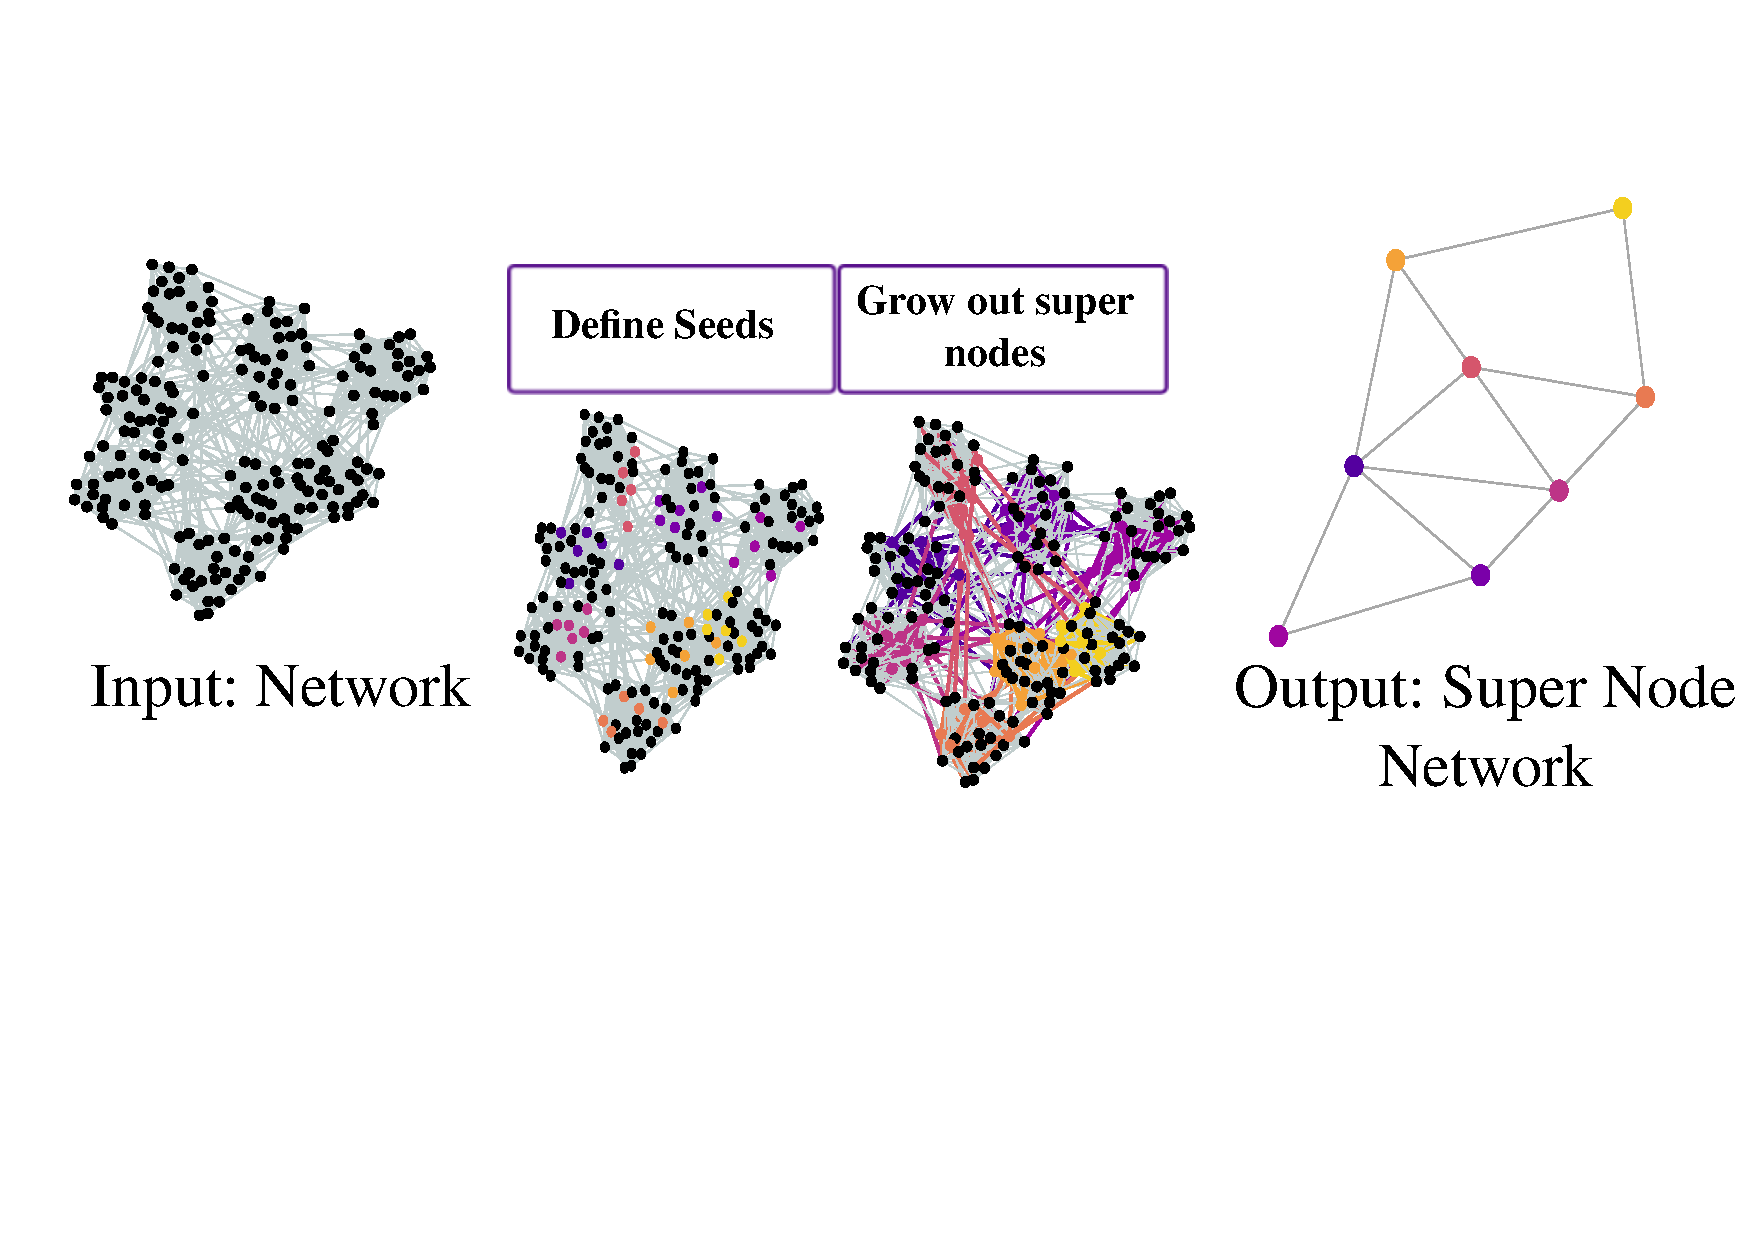
\includegraphics[scale=0.4]{Schematic_smaller.pdf}
\caption{{\bf Defining super nodes}. To define the super node representation of a network, we select $S$ seeds and agglomerate local regions around them to create super nodes. This then leads to a new network with weighted edges between the $S$ super nodes upon which community detection can be more efficiently applied.}
\label{Fig1}
%\end{center}
\end{figure}

\subsubsection{Objectively Comparing Partitions on Possibly Different Scales}
A challenge in directly comparing the community partitions on the full and super node network representations is the difference in scales between the partitions. For example, using the full network typically produces significantly more communities than under the super node representation. In an attempt to compare community partitions with similar size distributions in the subsequent experiments, we can adapt the scales obtained from the Louvain algorithm and SBM fitting.

In community detection with the Louvain algorithm, we identified comparable resolution parameters (controlling community size) to apply to the full network that would produce a size distribution agreeing as much as possible with the community partition in the super node network. We compute experimental results using both the default resolution parameter and the `matched' parameter. While the default resolution parameter is $\gamma=1$, in our analyses we computed partitions of the full network using several different $\gamma\in[0.05, 2.5]$. To choose the matched resolution parameter on the full network, we first find the community partition using the super node representation. For each partition, we then order nodes based on the sizes of the communities to which they belong. With this approach, all nodes from the same community are at the same position in the ordering. For each partition of the full network (at different resolution parameters), we then consider the similarity of this ranking with that from the super node communities, measuring this similarity by Kendall's tau correlation. We identify the resolution parameter producing the highest Kendall's tau correlation, referring to this resolution parameter as the `matched parameter' in the remainder of the text, while we refer to the standard $\gamma=1$ as the `default' resolution parameter.

In fitting SBMs, we chose to fit a model with the same number of blocks that was found in the super node representation using the standard optimization and model selection strategies discussed in Ref.~\citenum{tiagosbm}. We refer to the `matched' version as that using the number of blocks identified by the model selection on the super node representation, while the `default' result is obtained using the model selection strategy on the full network. In subsequent experiments, we compare both the `matched' and `default' versions to ensure our results are not artificially influenced by the scale of the community sizes.

\section{Methods}
We create a super node representation through three steps, outlined in Figure \ref{Fig1}. First, we define seeds. Next, we `grow' super nodes by assigning the remaining nodes to seeds. Finally, the network of super nodes is defined by agglomerating edges, and can then be used in a community detection algorithm. 
\subsection{Defining seeds}
To define $S$ seeds, we aim to identify a set of nodes $S^{*}$ that are individually central to the network and to their communities, and that are well separated from one another. Such problems are related to influence maximization, where one identifies a small number of nodes in the network from which to effectively spread influence or diffuse messages across the network \cite{jungirie,kempe}. The most naive approach is to select nodes with highest degree, and this might be perfectly reasonable under various circumstances. Importantly, the selection of nodes with highest degree is computationally fast, requiring $O(M)$ operations, summing over the $M$ edges to calculate the degrees of the $N$ nodes. 

At slightly higher computational cost, we employ the CoreHD algorithm, which nearly optimally identifies nodes in network decycling and dismantling \cite{CoreHD}. CoreHD recursively identifies the highest degree node in the 2-core (the maximal connected subgraph in which all nodes have degree at least 2 within the subgraph, obtained efficiently by recursively pruning away all nodes of degree less than 2). At each iteration, the removed node is added to our seed set and the now smaller 2-core and their degrees are recomputed. The difference between selecting highest degree nodes and CoreHD for our present task may be small, both in terms of result and computational cost. In particular, because we will only select $S\ll N$ seeds, there is reduced opportunity for the removals to lead to subgraphs with substantial differences between degree order in the graph and its 2-core [cf.\ selection of $O(N)$ removals in network dismantling]. Indeed, in our experience, simply selecting the highest degree nodes as the seeds often works well in practice. Because of the minimal extra computational cost for computing the 2-core, we use CoreHD for all of our results shown here. In Figure \ref{Synth}, we plot a sample network generated from the stochastic block model, with nodes colored according to community assignments and black nodes indicating seeds, showing the seeds are distributed across all 8 communities. 

\begin{figure}
\centering
%\begin{center}
%\centering
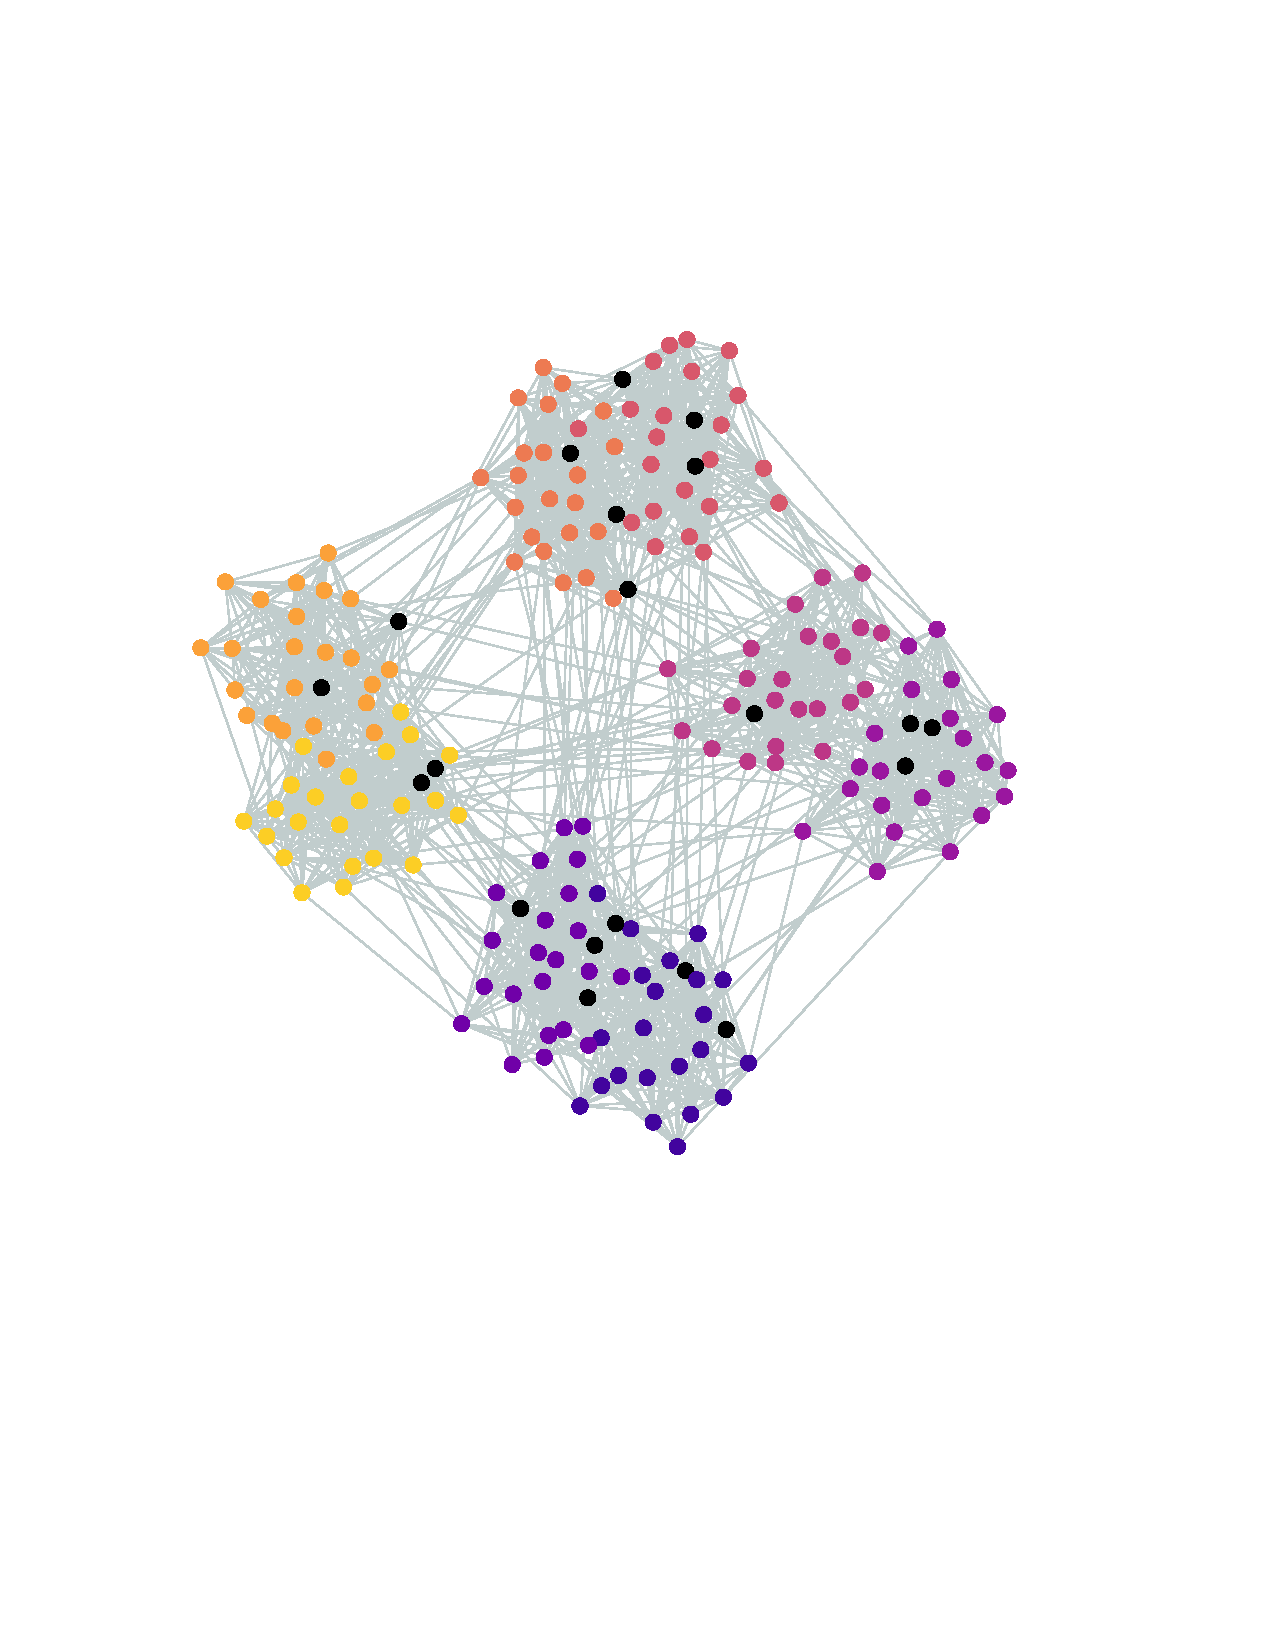
\includegraphics[width=0.25\textwidth]{Synthetic}
\caption{{\bf Choosing seeds in a synthetic network}. The identification of 20 seeds with the CoreHD algorithm in a network generated from a stochastic block model with 8 communities. Seeds (black nodes) are well distributed across communities.}
\label{Synth}
%\end{center}
\end{figure}

\subsection{Grow Super Nodes Around Seeds}
Once the set of seeds, $S^{*}$, is defined, we `grow' them out  agglomerating nearby nodes to build the super nodes. We formally define a super node as a subset of one or more nodes from the original network, ${\mathcal X}$. To do this, seeds are grown out to engulf nodes in increasing neighborhood orders until either all nodes are assigned to a super node center or until a user-defined number of neighborhood orders has been considered. The maximum order, $o_{max}$, can be specified to control the maximum order neighborhood to consider in building the super nodes. If after $o_{max}$, there are still unassigned nodes, the unassigned nodes are not used to build the new super node network and are all ultimately assigned to the same periphery community as they are not considered relevant to the network core.  Depending on the number of chosen super nodes, $S$, the degree distribution of the original network and the quality of the chosen seeds at collapsing the network, different networks will require repeating the agglomeration process for different neighborhood orders if one wants to ensure every node is assigned to a super node.  %This function takes as input the full network, ${\mathcal X}$ and the chosen set of super nodes, $S^{*}$.  
The output is a vector, ${\bf s}$ of length $N$, which gives the node-to-super-node assignments for the nodes in the original network. 

\subsection{Create Network of Super Nodes}
Finally, after growing the super nodes, we create a new network representation of the super nodes. To do this, we create a weighted network, $\mathcal{W}$, where each super node is a node and the weight of the edge between a pair of distinct super nodes is the total weight of edges in the original network ${\mathcal X}$ between pairs of nodes assigned to the respective  super nodes. For pairs of super nodes whose members have no edges between them in ${\mathcal X}$, there is no corresponding edge in ${\mathcal W}$. By definition, we construct ${\mathcal W}$ with no self loops. Moreover, the produced super node network representation produces a weighted network where the edge weights are counts. 

After applying community detection to the super nodes, their community assignments are mapped back to their constituent $N$ nodes of the original network, ${\mathcal X}$. We denote this final $N$-length matched community assignment as ${\bf z}$. In experiments in the Results section, we consider the node-to-community assignment ${\bf z}^{Full}$ obtained by applying community detection to the full network and the mapped result ${\bf z}^{SN}$ obtained by applying community detection to the super node representation.

\section{Results}
To demonstrate the effectiveness of super nodes, we performed experiments to analyze the runtime, partition variability, alignment of communities with local network connectivity, and agreement with the communities obtained from the full network. We considered 9 unweighted network data sets (see Table~\ref{table:dataset})  from the Stanford Network Analysis Project database\cite{snapdata}
%\footnote{\url{https://snap.stanford.edu/data}} 
(Enron, Amazon, Dblp, 
\begin{table}.   %{.5\textwidth}
\begin{center}
\scalebox{0.7}{
\begin{tabular}{ |c|c|c|c| } 
%\caption{Summary statistics for networks used in experiments.}
\hline
\textbf{Dataset} (* indicates subgraphs) & \# Nodes & \# Edges \\
\hline
As22* (Internet)  & 22,801 & 48,270 \\ 
Enron* & 32,374 & 178,195 \\ 
CMatter* (Condensed matter 2003 collab.)& 17,816 & 83,337\\ 
Dblp* (com-DBLP) & 150,801 & 639,330\\
Amazon* (com-Amazon) & 77,463 & 209,887\\
Email (email-EuAll) & 265,214 & 420,045\\
Stanford (web-Stanford) & 281,903 & 2,312,497 \\
Notre Dame (web-Notre Dame) & 325,729 & 1,497,134\\
BrightKite (loc-BrightKite) & 58,228 & 214,078 \\
\hline
\end{tabular}
}
\end{center}
\caption{Network data characteristics.\label{table:dataset}}
\end{table}
Email, BrightKite, Stanford, Notre Dame) and Newman's collection\cite{newmandata}
%\footnote{\url{http://www-personal.umich.edu/~mejn/netdata/}} 
(As22, CMatter). We treat all networks as undirected. To explore a range of network sizes, in some of these cases we used large subgraphs defined by the union of all nodes of degree $\geq 2$, their neighbors, and next nearest neighbors. We use the Louvain algorithm\cite{traaglouvain}
%\footnote{as implemented in \url{https://github.com/vtraag/louvain-igraph}} 
for modularity maximization \cite{blondel} and the stochastic block model (SBM) inference\cite{tiagoskewed}
%\footnote{as implemented in \url{https://graph-tool.skewed.de/}} 
described in Ref.~\citenum{tiagosbm}. Since the super node representation ultimately produces a weighted network, where the edge weights are counts computed based on the original network, both of these community detection are able to accommodate these kinds of edge weights. 

\subsection{Overview of experiments}
Because we consider a variety of comparisons between partitions under different community detection methods and network representations, we provide a schematic in Figure \ref{concept} of the comparisons we performed in  Figures \ref{FigQuality} and \ref{VAR}. In these comparisons, we use normalized mutual information (NMI) to quantify the similarity between a pair of partitions.  In general, there are four possible combinations of community detection method/ network representation that can be applied to identify communities. First, there are two choices of community detection algorithm, Louvain algorithm or stochastic block model fitting. There are also two choices for network representation, which is to use either the full network or super node network representation. In Figure \ref{concept}, we represent a single partition of the network by a circle. Due to the stochastic nature of the community detection methods, it is useful to consider multiple runs (i.e. partitions) of the algorithm. The circles in the diagram are colored by one of the four network/method combinations. We assume that under each network/method combination, we generate multiple partitions. Amongst all partitions, we perform our analyses on all pairs of network partitions generated tat satisfy our comparison criteria. The first partition comparison we consider is shown in Figure \ref{concept} A., and seeks to quantify the similarity between a set of partitions generated with different network representations under the same community detection algorithm. The comparison computes NMI$({\bf z}^{Full},{\bf z}^{SN})$. For example, we could consider the pairwise similarity between the full network and super node representations with the stochastic block model. This comparison helps to understand how well the super node representation can be used to estimate the node-to-community assignments that could have been obtained using the full network. Next, we explore the inherent variability of community detection algorithms, which seems to especially arise among partitions of a large network. Figure \ref{concept} B. considers pairs of partitions under the same network representation and community detection algorithm. For example, we may run the Louvain algorithm on the super node representation of the network multiple times and compare all pairs of partitions. Finally, in Figure \ref{concept} C., we consider pairs of partitions generated under the same network representation but with different methods. In one example, we may compare partitions of the full network representation, where one partition used the Louvain algorithm and the other is obtained by fitting an SBM. Since these methods are different by design, they should still capture sufficiently common structures.

\begin{figure}
\begin{center}
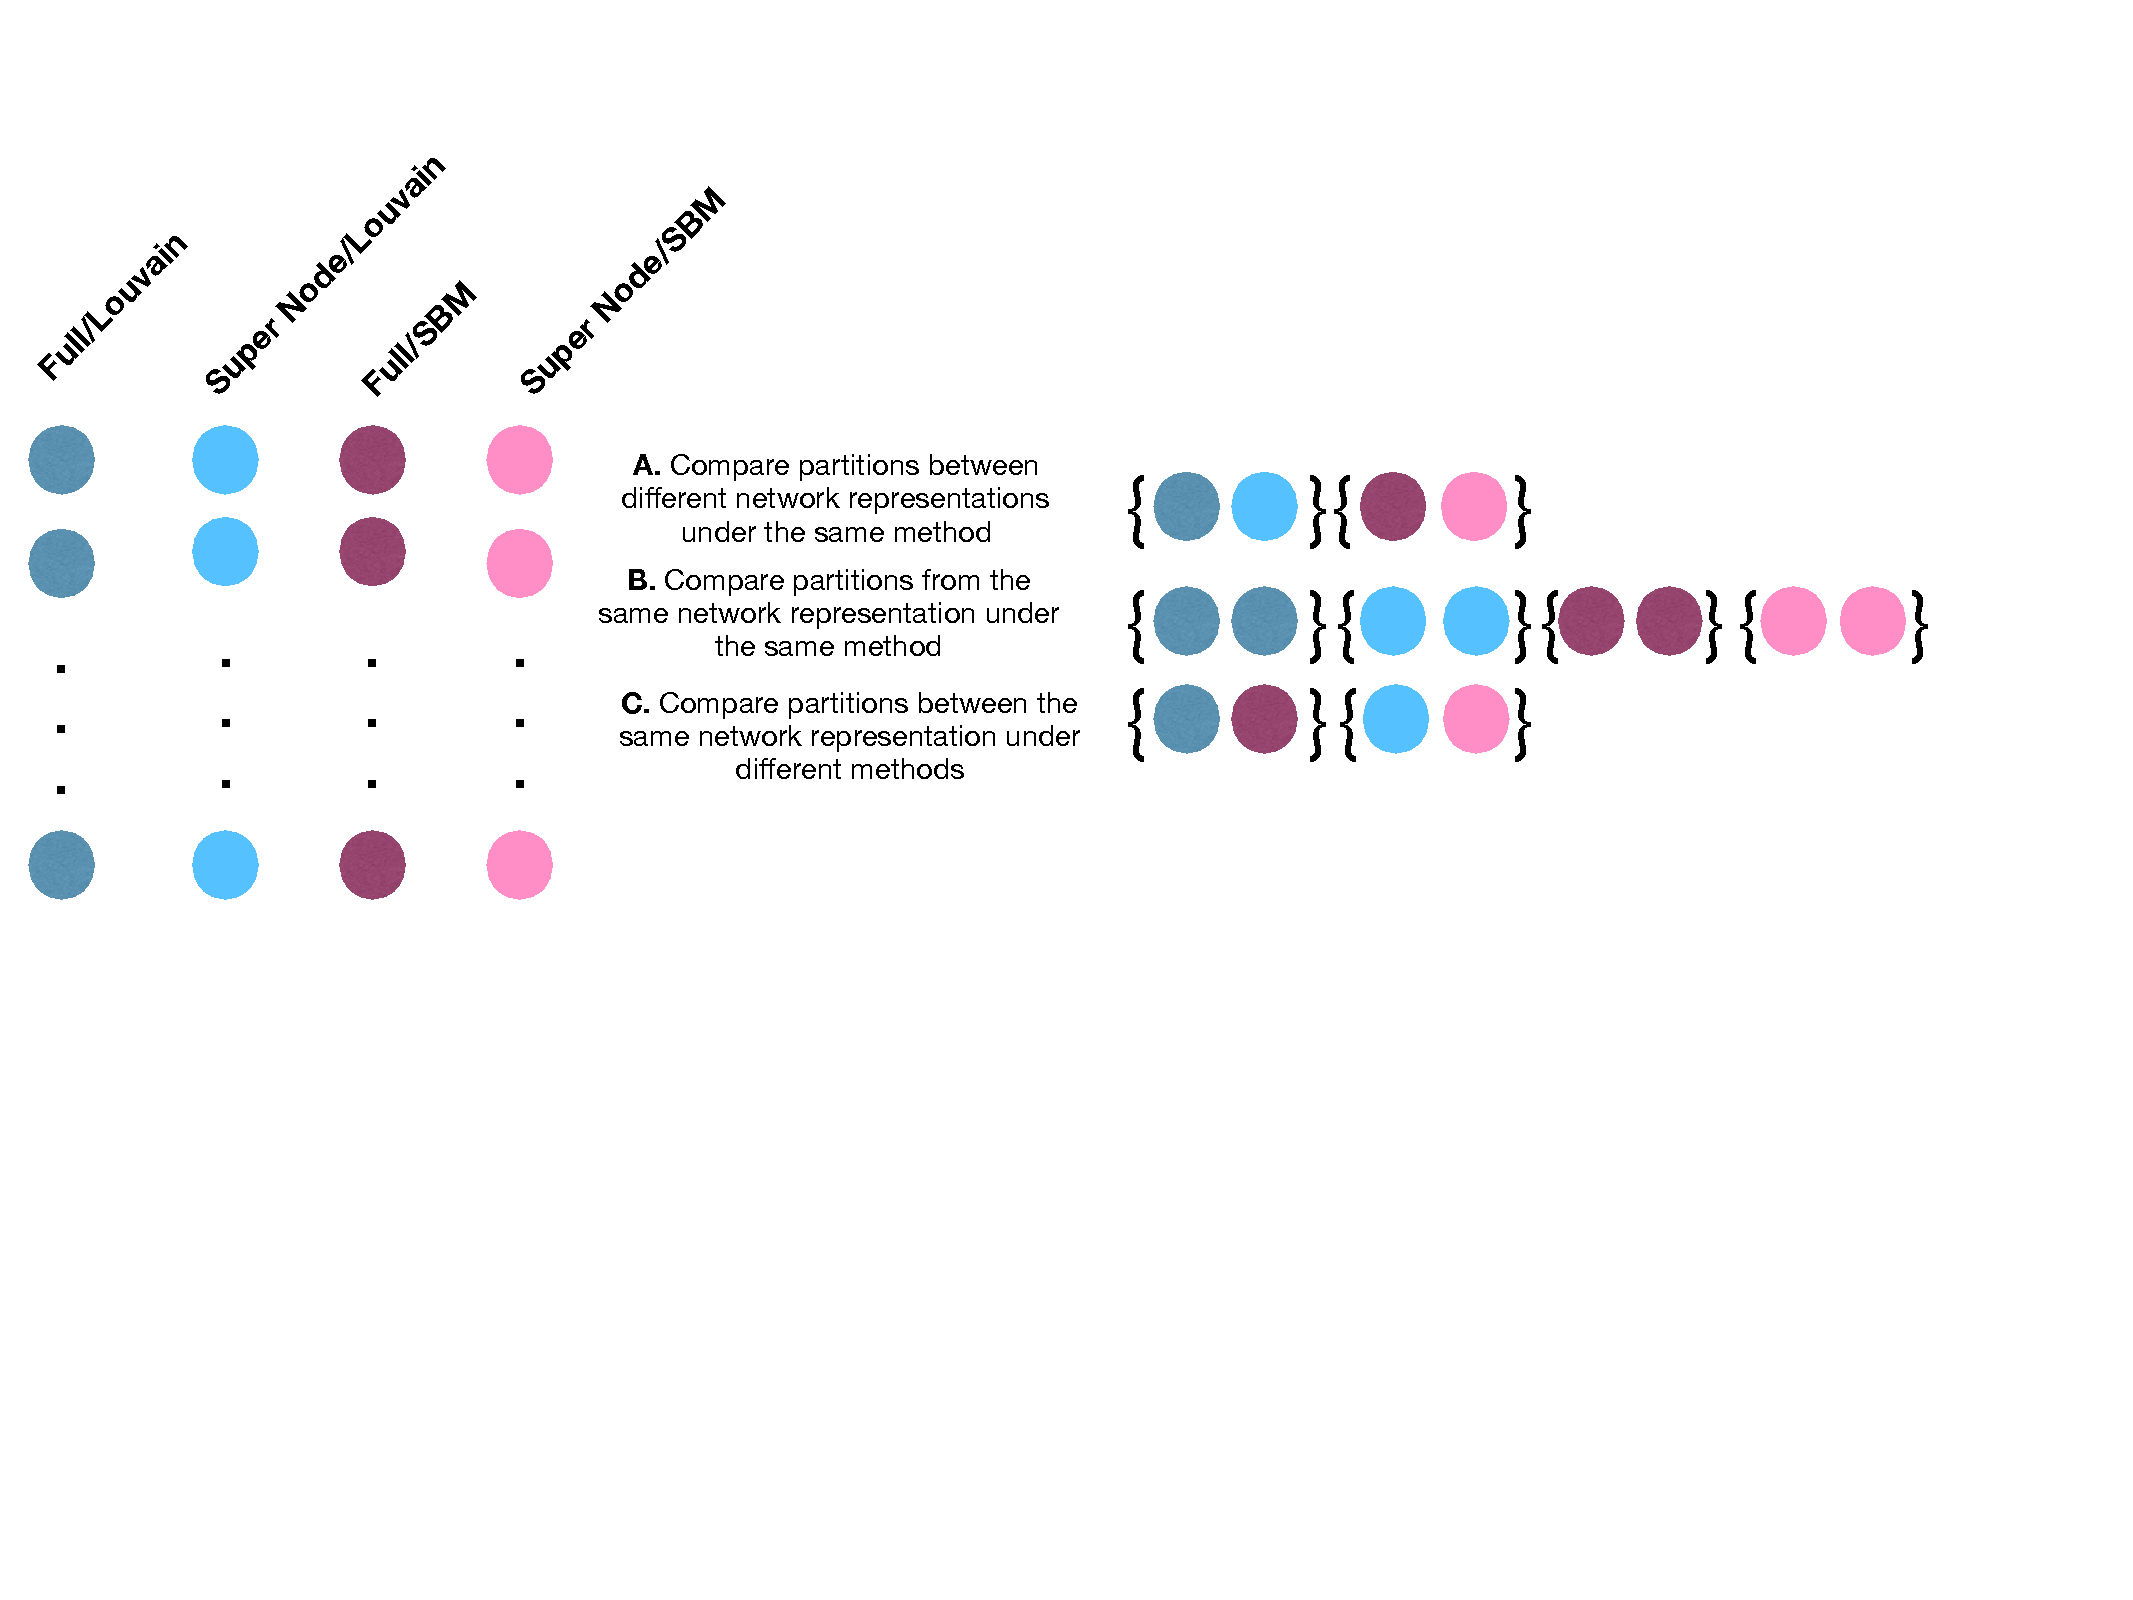
\includegraphics[scale=0.35]{Conceptual}
\caption{{\bf Schematic of possible partition comparisons.} We outline the types of possible comparisons between partitions generated according to various combinations of network representation and community detection method. According to these comparison rules, we compute normalized mutual information (NMI) between all pairs of networks satisfying the comparison criteria. The colored circles in the schematic represent a single partition generated under the corresponding  network representation and community detection algorithm combination. Circles are colored (in each column) by each of the four possible representation/community detection method combinations. In {\bf A-C}, we outline the types of comparisons we perform in subsequent figures. {\bf A.} To compare the usefulness of the super node representation in identifying communities retrieved using the full network, we compare pairs of networks with different representations under the same community detection algorithm. {\bf B.} Due to the stochastic nature of both the Louvain algorithm and SBM fitting, this comparison seeks to quantify partitions generated under the same network representation and method. {\bf C.} Finally, we consider pairs of partitions generated under the same network representation and different community detection algorithms. }
\label{concept}
\end{center}
\end{figure}

\subsection{Normalized mutual information and under segmentation error}
First we measure the quality of the super node representation in terms of NMI and under segmentation error that were defined in equations \ref{UnderSeg} and \ref{NMI}. In Figure \ref{FigQuality},  we vary the number of super nodes  and examine the normalized mutual information (A.) (equation \ref{NMI}) and log under segmentation error (B.) (equation \ref{UnderSeg}) in each of the 9 networks. The curves represent the mean NMI (A.) and mean under segmentation error (B.) over 5 super node representations, with the shaded area denoting standard deviation. Varying the number of super nodes between 100 and 600, the results generally indicate that as the number of super nodes increase, the network has 1) lower under segmentation error and 2) higher NMI (i.e. similarity) with the partition obtained using the full network. Each curve and line type in Figure \ref{FigQuality}  specifies whether community detection was performed using the Louvain algorithm or by fitting an SBM. To give some intuition about what value of NMI is considered good, we put our results in the context of the partition variability among 10 runs of the same community detection algorithm. In Figure \ref{FigQuality} A., we indicate the mean pairwise NMI between multiple runs of the Louvain algorithm and SBM fitting with horizontal pink and gold lines, respectively. This comparison is that described in Figure \ref{concept} B. Since in most cases, the pairwise NMI between partitions is not 1, by increasingly adding super nodes, we can only expect to asymptotically approach the mean pairwise NMIs. between multiple runs of the same algorithm on the original full network representation. Randomly permuting the node-to-community assignment obtained under the super node representation 1000 times and computing the NMI with the full network (i.e. NMI$({\bf z}^{Full},{\bf z}^{SN})$) gives a mean NMI on the order of 0.01. 
\begin{figure}[t!]
\centering
%\begin{center}
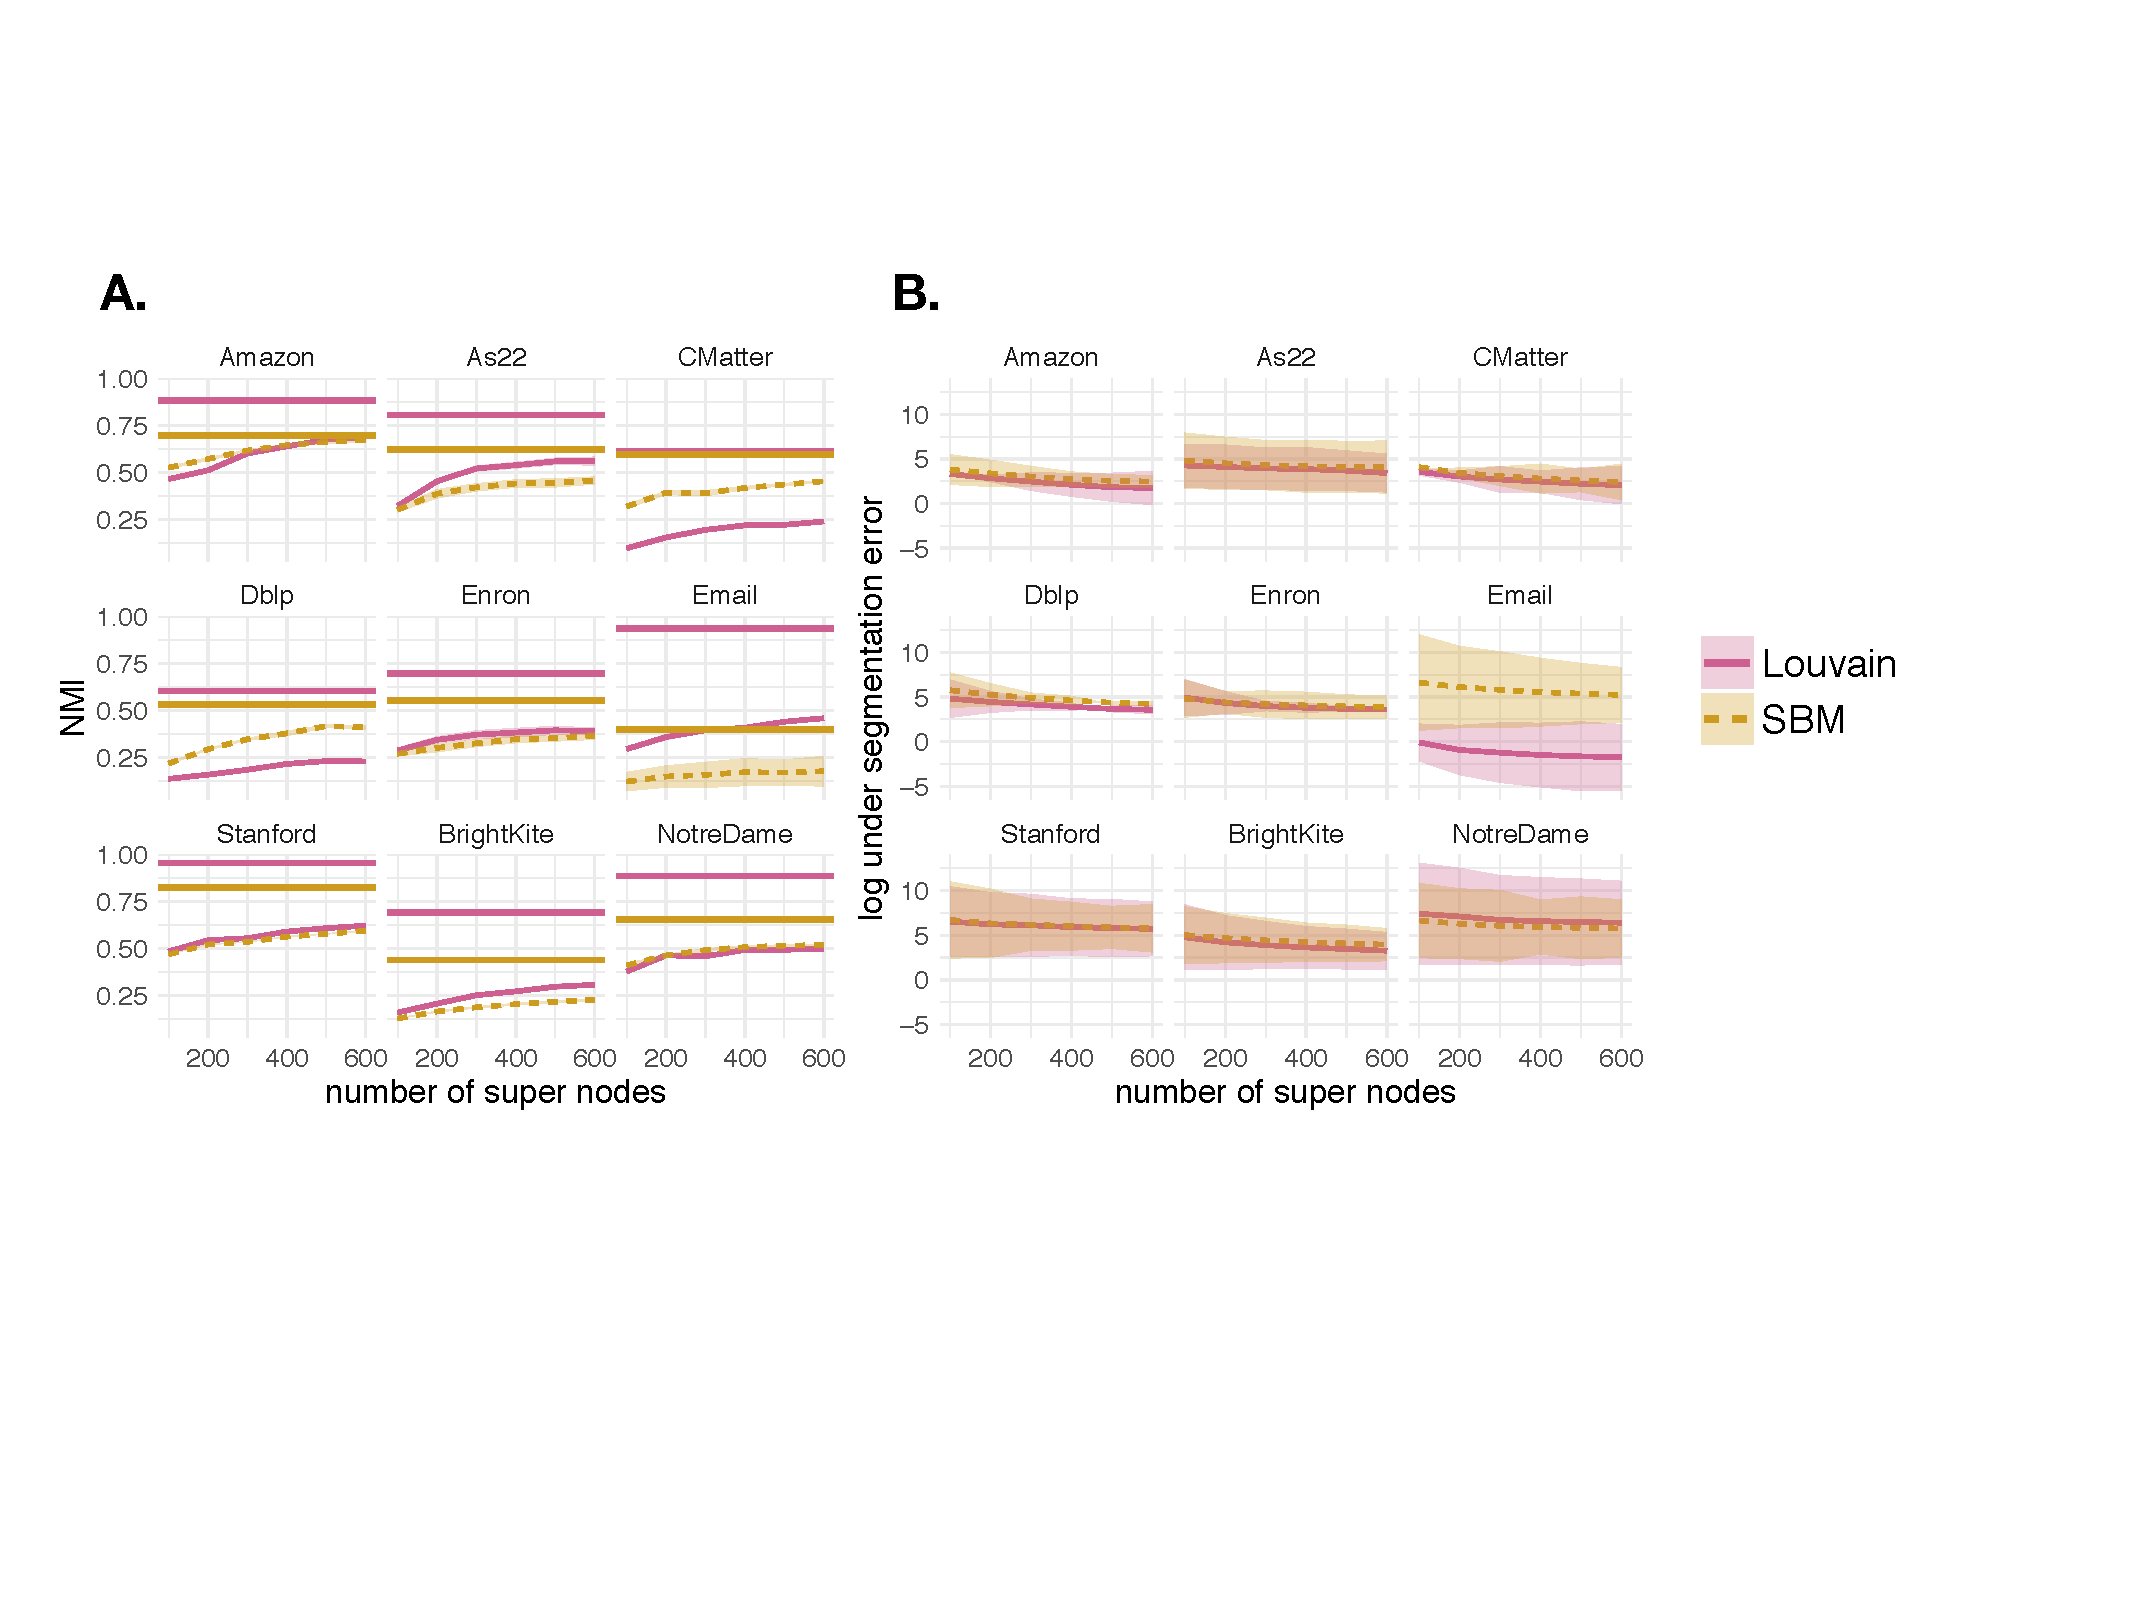
\includegraphics[scale=0.5]{NMI_UnderSeg}
\caption{{\bf Super Node Quality.} We computed normalized mutual information ({\bf A.}) and under segmentation error ({\bf B.}) for networks represented by between 100 and 600 super nodes. Line type and color indicate the community detection algorithm applied (Louvain algorithm or SBM fitting). Each curve indicates the mean across 5 super node representations. The shaded area shows standard deviation. {\bf A.} Normalized mutual information between the full and super node representations of networks [i.e. NMI$({\bf z}^{Full},{\bf z}^{SN})$]. A network representation with more super nodes. generally increases the NMI between full network and super node network representations. Horizontal lines indicate the mean pairwise NMI between 10 runs of the Louvain algorithm and SBM result on the full network (pink and gold, respectively). Given the high variability between multiple runs of the same algorithm on the full network, adding more super nodes can only improve the NMI between the full and super node representation to the observed level of similarity observed between algorithm runs. {\bf B.} The log under segmentation error for super node representations. Defining a super node representation with more super nodes generally decreases the under segmentation error. }
\label{FigQuality}
%\end{center}
\end{figure}

\subsection{Run time Analysis}
In practice, one of the most desirable properties of a super node representation of the network is the decrease in the run-time of community detection algorithms in comparison to using the full network. For each of the 9 networks, we recorded the runtime required to identify communities with the Louvain algorithm and stochastic block model inference procedure under the full a 500 node super node network representations (Figure \ref{RT}). The Louvain algorithm is fast and scales well, at $O(M)$ per iteration for $M$ edges, with its relative speed and high modularity values contributing to its popularity. While the reported runtimes may seem quite modest, in practice it is common to run many realizations of the algorithm (hundreds, thousands, or even more for large networks) to explore resolution parameters and stochastic variation due to pseudorandom node order in the heuristic. We note a large increase in runtime for the full Stanford network, with over 2 million edges. As also observed in the figure, fitting a stochastic block model, at $O(N{\ln}^{2}N)$ for sparse networks in this implementation,\cite{tiagosbm} becomes significantly slower on the full networks with more than 200,000 edges. 

While we see a significant improvement in community detection runtime from using super nodes for both methods, the benefit in the SBM fitting is particularly large, especially for the bigger networks (DBLP, Stanford, Email). In moving to the super node representation, we traded out large-coefficient scaling-with-$N$ community detection computations for those scaling with $S\ll N$ (with possible increases due to the increased density of the super node representation), at the cost of constructing the super node representation. In particular, we observe the SBM runtimes on super nodes appear to be relatively independent of $M$. We note that each of the three steps building our super-node representation is $O(M)$, so in the large graph limit the expected gain of our approach may be only a constant factor over Louvain iterations and the SBM fitting (up to logarithmic factors). In the present calculations, we have not endeavored to optimize the runtime to build our super node representations; even so, the three steps building the $S=500$ super node representation of the Stanford network in our current implementation together take $\sim 350$ sec with CoreHD and $\sim 200$ sec using highest-degree nodes. While this alone might not seem like a large improvement compared to a single realization of running Louvain or fitting an SBM, the computational gains compared to generating multiple community partitions can be quite significant.  %That is, that, while $O(M)$ in the large-graph limit, is all but negligible at the scales of our present examples, especially in the setting where each super node representation may be used many times to study variability across community detection runs and for different resolution parameters.  
 
\begin{figure}
\centering
%\begin{center}
\includegraphics[scale=0.6]{RunTime}
\caption{{\bf Runtimes}. We compare community detection runtimes (in seconds) with the Louvain algorithm and by fitting an SBM on the full networks and super node representations for the 9 data sets. {\bf (A.)} Louvain on the full network. {\bf (B.)} Louvain  on the super nodes. {\bf (C.)} SBM on the full network. {\bf (D.)} SBM on the super nodes.}\label{RT}
%\end{center}
\end{figure}

\subsection{Quantifying variability across algorithm runs}
As mentioned previously, there is variability in the partitions generated by multiple runs of the same community detection algorithm on the same network representation. We sought to quantify how the variability or pairwise similarity between multiple runs of the same algorithm changes as a function of the number of super nodes in each network representation under the default and matched algorithm parameters (Figures \ref{VAR} A. and B.), respectively. Note that A. and B. show the same analysis with the only difference being the parameters input to the community detection algorithm. Curves represent the mean pairwise NMI between all pairs of 10 computed partitions under the super node network representation and shading shows standard deviation. The pink and blue curves show the within-method comparisons on the super node network representation for the Louvain algorithm and stochastic block model, respectively. That is, these are the comparisons shown in Figure \ref{concept} B. We were also interested in the variability of the partitions obtained between partitions of the super node representation found with different algorithms. This result is shown in the gold curve and labeled `Louvain+SBM'. Note that this analysis is described in Figure  \ref{concept} C. The horizontal lines show the mean pairwise similarity observed between all 10 runs of the Louvain algorithm and stochastic block model (pink and blue, respectively). The most significant improvement we observe under the super node representation is between runs of the Louvain algorithm and SBM fitting, suggesting that the new compressed representation of the network has prominent structural features that are robustly identified with both approaches. A high normalized mutual information between a pair of partitions indicates that the algorithms identified similar community structures.  The Louvain algorithm is generally less variable than fitting an SBM, but we also observed decreased variability in the fitting of stochastic block models on the super node representation. 

\begin{figure}
%\begin{center}
\centering
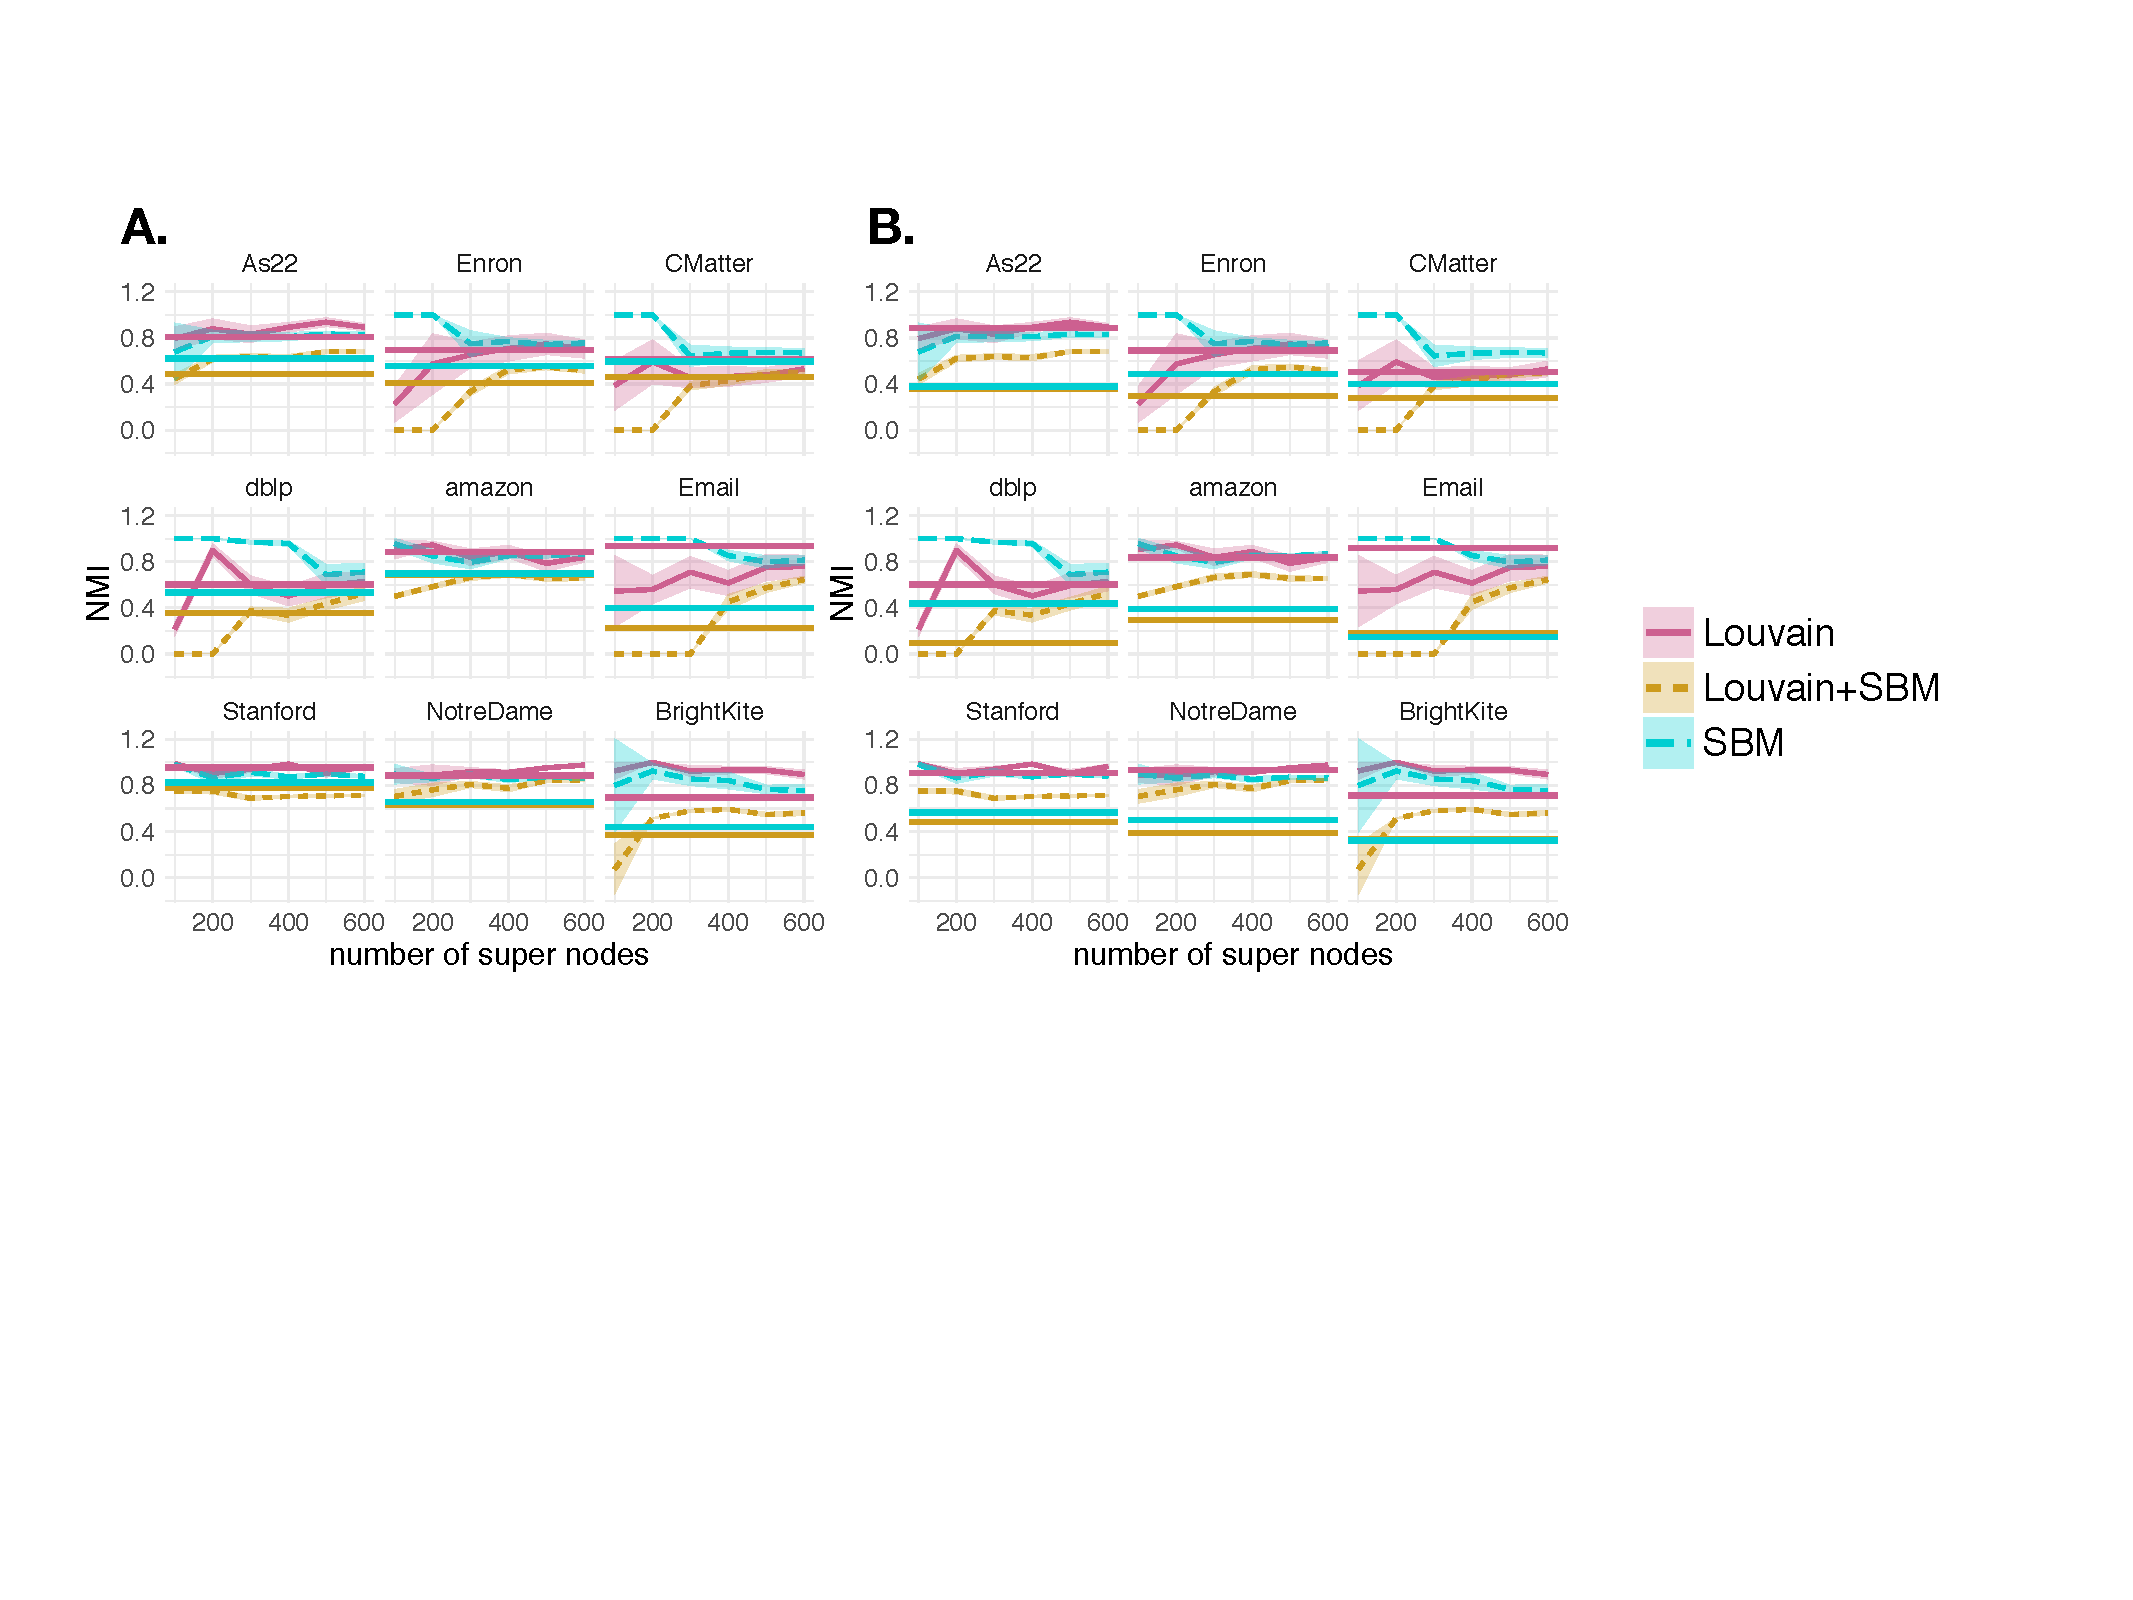
\includegraphics[scale=0.5]{VariabilityFigBoth.pdf}
\caption{{\bf Quantifying partition variability.} For each of the 9 networks, we obtained 10 different partitions by the Louvain algorithm and 10 different SBM fits under the default ({\bf A.}) and matched settings ({\bf B.}). To assess the similarity between partitions within and between a community detection algorithm in networks under the the super node representation, we computed pairwise normalized mutual information (NMI) as a function of the number of super nodes. The pink and blue curves show the mean pairwise normalized mutual information between all pairs of 10 partitions under Louvain and SBM fitting, respectively. The gold curves compare pairs of partitions under different methods. Shaded area denotes standard deviation. Horizontal lines indicates the mean pairwise NMI between partitions under the full network representation for within Louvain and SBM partition comparison (pink and blue, respectively) and between Louvain and SBM partition comparison (gold). Overall, the super node representation is useful for reducing the disparity between the partitions obtained under different methods.}
\label{VAR}
%\end{center}
\end{figure}

\subsection{Neighborhood agreement}
While we have emphasized benefits in the mechanics and usability of running standard community detection algorithms, we now seek to address whether the communities that we find using the super node representation align with local network connectivity so that neighbors are more likely to have similar community assignments and how this alignment compares with what we would have found by community detection on the full network. While we visualize this qualitatively for the As22 network in Figure \ref{Viz}E-H, we also designed a prediction task to quantify this alignment. In this prediction task, we seek to take a node-to-community partition (from either the full or super node network representations ${\bf z}^{Full}$ or ${\bf z}^{SN}$, respectively) and the full network ${\mathcal X}$ to see how accurately we can predict members of a community for different neighborhood sizes.
For network ${\mathcal X}$ with node-to-community assignments ${\bf z}$, we assign a probability distribution to each node over all of the communities under ${\bf z}$. For a neighborhood order $o$ (x-axis in Figure \ref{Viz}), we say that node $i$ has probability of being in community $k$, based on what fraction of its neighbors belong to that community under ${\bf z}$. Then for each community in ${\bf z}$, we perform a binary prediction task for whether each node of ${\mathcal X}$ should be assigned to that community, according to the computed probability distributions for all nodes with respect to that community. 

We sweep the probability parameter, $p$, representing the required threshold probability for a node to achieve in order to be assigned to a community in this binary classification task. By sweeping $p$ for each of the communities, we compute an ROC curve for each community and the corresponding areas under the curve (AUC). Finally, we use the minimum AUC value as our summary statistic of this task, with a high AUC value indicating that the neighboring regions of a node were strong predictors of community assignments, as shown in Figure \ref{Viz}A-D. All experiments are performed on 5 networks (As22, Enron, CMatter, Dblp, Amazon) and for both the matched and default parameters (indicated by line type) in the full network. (Recall from section 3.1 that the matched parameters for the full network were chosen based on the super node partition results under default settings; hence, there is no corresponding `matched' set for the super nodes in these plots.) We observe in most cases using the super node representation improves the minimum AUC value, indicating that communities obtained from this representation have higher agreement with local connectivity by this measure.
\begin{figure}
\centering
%\begin{center}
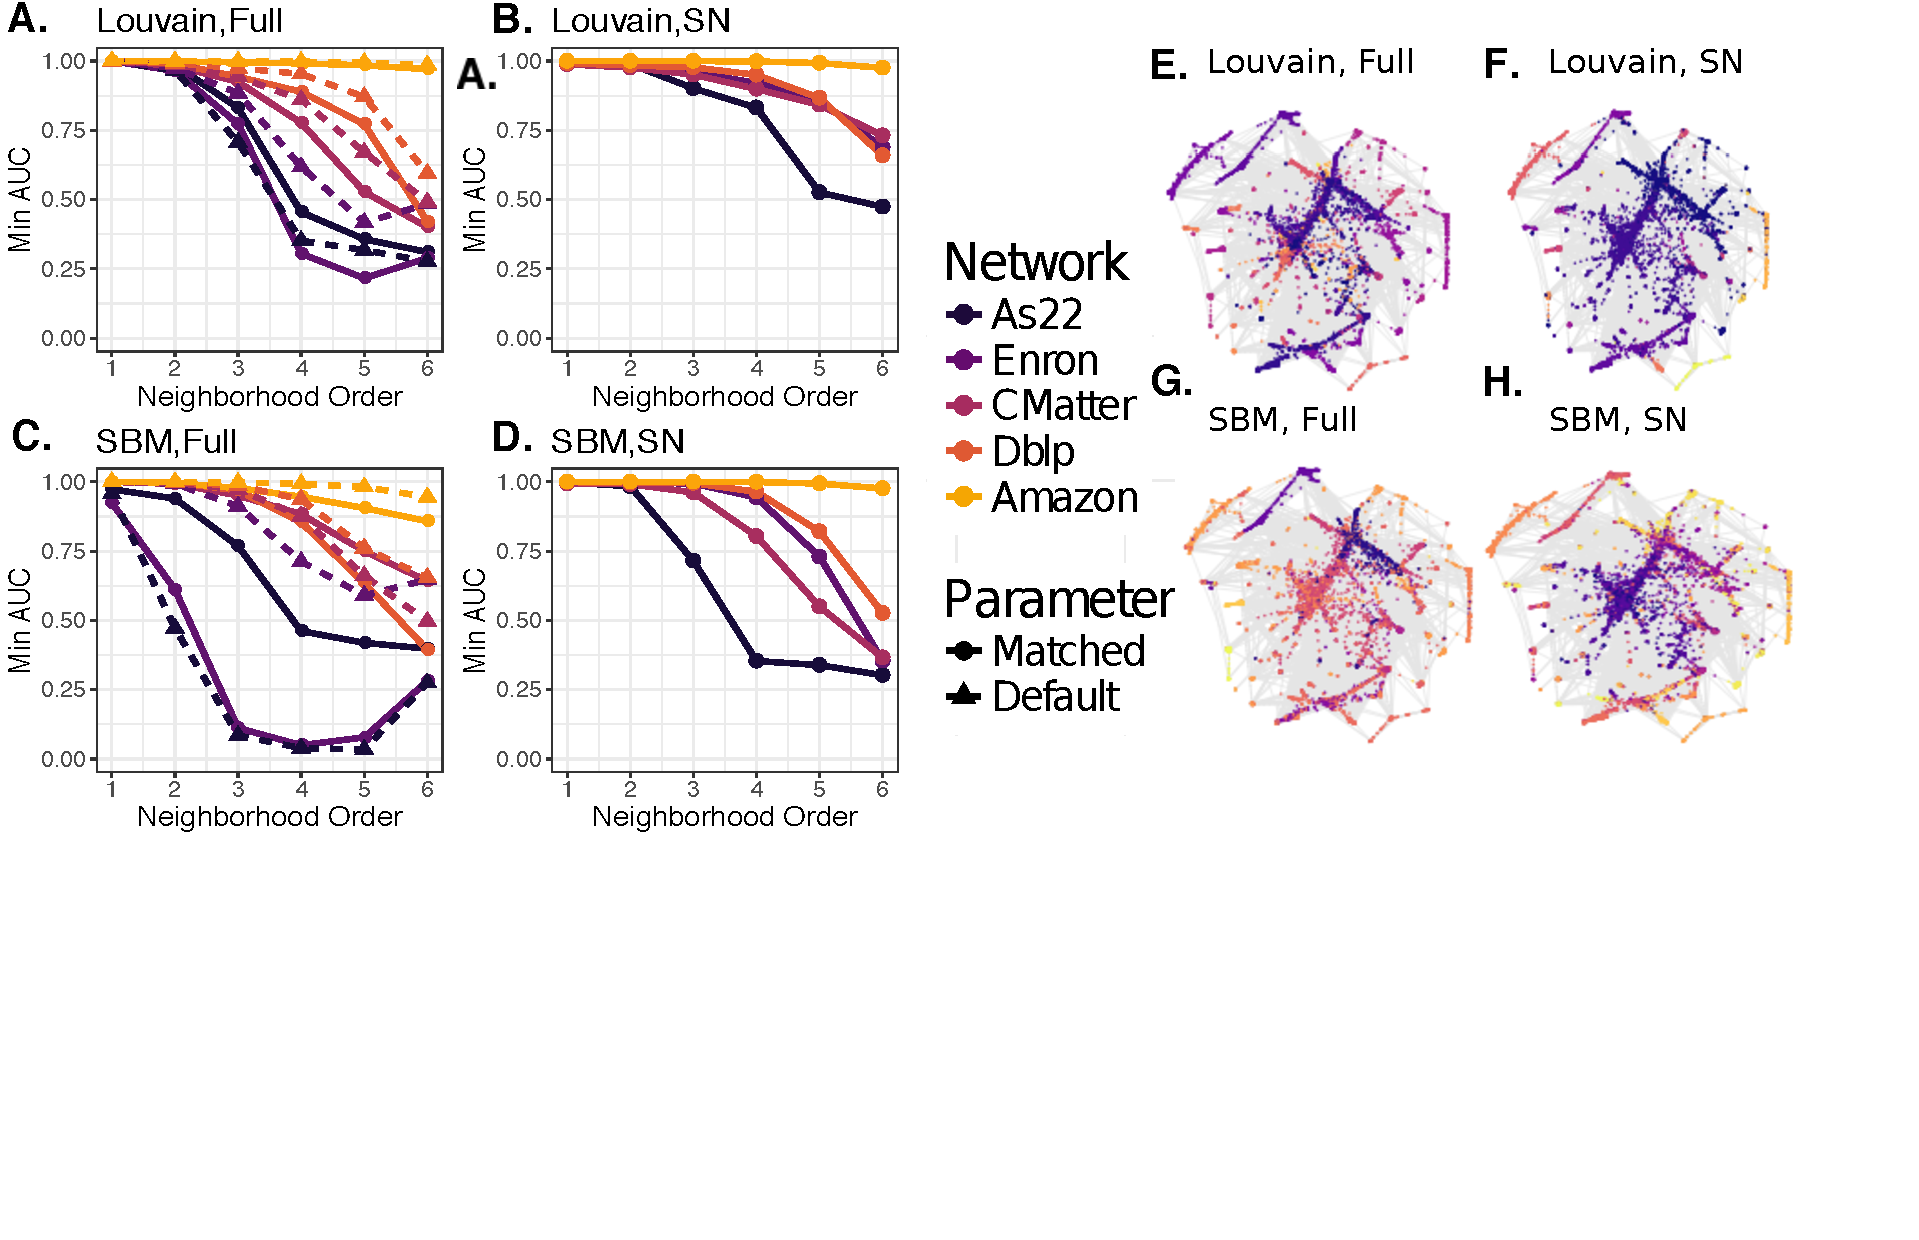
\includegraphics[scale=.5]{FinalAUC.pdf}
\caption{{\bf Agreement of community assignments with local connectivity}. We study how  consistent partitions are within local neighborhood regions of the network by examining how well a node's neighbors (for various order neighborhoods) can be used to predict its community assignment, under some community partition ${\bf z}$. For each community in a partition, we give a binary prediction of whether a node is assigned to that community, based on probabilities we compute for a node from its neighbors. Sweeping the parameter $p$ that sets the probability required for a node to be assigned to a community, we compute ROC curves for each community and report the minimum AUC value observed. Panels {\bf A-D} show minimum AUC values observed as a function of neighborhood order for communities obtained from the full networks and super node representations by Louvain and by SBM. Line color indicates network and line type indicates communities obtained from the matched and default parameters used by the algorithms on the full networks. Panels {\bf E-H} visualize the communities obtained in the As22 data on the full network (default parameters) and super node representation (SN) under Louvain and SBM, with node colors indicating community memberships. }
\label{Viz}
\end{figure}
To qualitatively evaluate how the super node representation is able to ultimately partition the network into communities that are locally relevant, we visualize the As22 network, with nodes colored by communities identified under the full network (E,G) and super node representation (F,H) under Louvain (E,F) and SBM (G,H). Consistent with the quantitative results in Figure \ref{Viz}A-D, we observe that the super node representation leads to an effective coarse-graining, with the community labels appearing to be qualitatively consistent across large regions of the network.

\section{Conclusion and Future Work}
\indent We developed an approach for compressing a network into a super node representation that can be used in standard community detection algorithms. Using the smaller super node network reduces runtime and the variability between multiple runs of the same community detection algorithm. Our results also demonstrate that the communities in the super node network are better aligned with local network neighborhoods in a predictive sense, while still being in relatively good alignment with the partitions obtained using the full network. \\
\indent Super nodes may be useful in a variety of contexts where large datasets are otherwise difficult to mine and interpret. For example, one might visualize the super node version of the network rather than the entire network, or use the members of a super node to identify redundant information in the network. Future work on super node representations could include the extension of this method to directed, signed, attributed, or bipartite networks. Additionally, one might consider a probabilistic model framework, attempting to infer latent super node assignments. 
Future work could also examine graph theoretic properties of super node representations in terms of how it aligns with the original network. 

\chapter{An attributed stochastic block model}
\indent While community detection is an inherently unsupervised problem, there are often circumstances where there is extra information about the nodes, or node attributes. In this case, the clustering problem of grouping nodes into communities becomes a problem of integrating two different types of data. There have recently been numerous discussions as to what extent it makes sense to assume that members of a community according to connectivity should also have similar attributes. In particular, we address the case where each node has multiple continuous attributes. To build a model that takes into account both sources of information, we extend the classic stochastic block model to take into account continuous attribute information, when inferring node-to-commumunity assignments. In the process of assigning nodes to communities, we learn probabilistic models describe both the attributes and connectivity. We then use these learned models to perform link prediction and collaborative filtering tasks. 

\section{Motivation for studying attributed networks}
\indent In certain applications, each node in a network is equipped with additional information (or particular attributes) that was not implicitly taken into account in the construction of the network. For example, one could consider a collection of attributes measured for individuals in a social network (i.e., age, interest, level of education). The interplay between the connectivity-based (or structural) community organization of the network and attribute information has gained attention, as it is often unclear whether it is valid to assume that a \emph{structural} community should necessarily correlate with an attribute-based \emph{functional} community \cite{hric,peel2017ground,jureTruth}. While these studies suggest that extreme caution should be taken in assuming a correlation between structural and functional communities, we limit our focus in this work to the assumption that a node's connectivity and attribute patterns can be jointly modeled based on its community assignment. In other words, we seek to develop an approach to assign node to communities based jointly on both sources of information, such that a community is defined as a group of nodes with similar connectivity and attribute patterns. Moreover, our objectives are two-fold.  First, we seek to develop a probabilistic approach to jointly model connectivity and attributes. Second, we wish to ensure that our model can handle multiple, continuous attributes.  

\indent Recently, there have been numerous efforts to incorporate attribute information into the community detection problem \cite{cesna,clauset,ilouvain,hric,peel2017ground}. Two classes of community detection methods are quality function-based and probabilistic. Quality function based methods define a quantity of interest that an ideal partition would satisfy, while probabilistic methods identify communities through likelihood optimization and focus on the underlying statistical distribution for the observed network. A recent quality function-based method to handle multiple attributes is I-louvain \cite{ilouvain}. This method approaches the problem as an extension to the Louvain algorithm, which is the state-of-the-art scalable quality function modularity-based community detection method \cite{blondel}. The traditional modularity-based approach to community detection defines a null model for community structure under the assumption that there is not substantial structural organization in the network and seeks to identify a partition maximally different from this model through optimizing a quality function (modularity). The I-louvain method modifies the standard modularity quality function as to what they call 'inertia-based modularity'. This quality function incorporates the Euclidean distance between nodes based on their attributes. This work demonstrates in multiple examples how incorporating connectivity and attributes allows for a partition of nodes to communities that aligns with ground truth better than the results obtained based on connectivity or attributes in isolation.

Alternatively, there a variety of probabilistic approaches to handling attributed network data \cite{clauset,hric,peel2017ground,cesna}. Similar to our work in the sense that community membership is related to node attributes is CESNA \cite{cesna}. The objective in this approach is to learn a set of propensities or affiliations for each node across all possible communities, such that two nodes with similar propensities towards communities should have more in common in terms of connectivity and attributes. In this model, each node has a vector with multiple binary attributes. The affiliation model is useful and flexible because it does not enforce a hard partitioning of nodes into communities, which is useful in social network applications. In this inference problem, the connectivity and attribute information are used to infer a node's affiliations to communities and then models the probability of an edge between two nodes as a function of the similarity in their community affiliation propensities. 

In contrast to the affiliation model, the stochastic block model \cite{originalSBM} (at least the more standard variants of it), seeks to determine a hard partition for each nodes across communities and models edges between a pair of nodes according to their community assignments. The partition of nodes to communities through a stochastic block model framework is accomplished through maximum likelihood optimization. An of the stochastic block model was first explored by Clauset \emph{et al.}, \cite{clauset}, which adapts the classic stochastic block model to handle a single attribute with the assumption that attributes (referred to as metadata in their work) and communities are correlated. Next Hric \emph{et al.,}, developed an attributed SBM \cite{hric} from a multilayer network perspective, with one layer modeling relational information between attributes and the other modeling connectivity. The authors then seek to assign nodes to communities  maximizing the likelihood of the observed data in each layer. Finally, work of Peel \emph{et al.} made important contributions in 1) establishing a statistical test to determine whether attributes actually correlates with community structure and 2) developing an SBM with flexibility in how strongly to couple attributes and community membership in the stochastic block model inference problem \cite{peel2017ground}. 

The model that we seek to develop in this work is distinguished by its ability to fit a stochastic block model to networks, where each node has multiple continuous attributes. This model is most appropriate for circumstances where there is domain-specific evidence that members of a community should exhibit similarities in attributes. We highlight two examples of this, where we apply our model to a protein interaction network and a microbiome subject similarity network. Our paper is organized as follows. First, we will define our attributed SBM and an inference technique for fitting the model. Next, we test this approach on a synthetic example as well as two biological network examples. Since community detection methods are often difficult to validate due to the lack of ground truth information on the nodes, we use link prediction and collaborative filtering to quantify how well the attributed SBM represents the data.

\section{An Attributed Stochastic Block Model}
 In this section we provide the details for our version of the attributed stochastic block model and the inference procedure used to learn the model parameters. 
\subsection{Objective}
We seek to incorporate both connectivity (${\bf A}$) and attribute information (${\bf X}$) to infer node-to-community assignments, ${\bf Z}$. Note that for a network with $N$ nodes, $K$ communities and $p$ measured attributes, ${\bf A}$, ${\bf X}$, and ${\bf Z}$ have dimensions $N \times N$, $N \times p$ and $N \times K$, respectively. In particular, ${\bf Z}$ is a binary indicator matrix, where entry $z_{ic}$ is 1 if and only if node $i$ belongs to community $c$. We also define ${\bf z}$ to be the $N$-dimensional vector of node-to-community assignments.We assume that connectivity and attributes are conditionally independent, given the community membership label. The graphical model for the relationship between node-to-community labels, connectivity and attribute information is shown in \ref{fig:graphical_model}.

\begin{figure}
\begin{center}
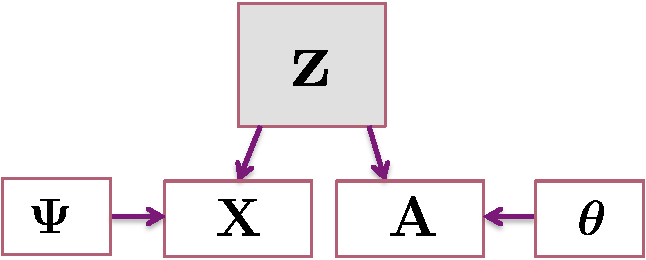
\includegraphics[scale=0.5]{GraphModel.pdf}
\caption{{\bf Modeling community membership in terms of attributes and connectivity}. Node-to-community assignments specified by ${\bf Z}$ are determined in terms of adjacency matrix information, ${\bf A}$ and attribute matrix information, ${\bf X}$. ${\bf A}$ and ${\bf X}$ are assumed by be generated from a stochastic block model and a mixture of multivariate Gaussian distributions, parameterized by ${\boldsymbol \theta}$ and ${\boldsymbol \Psi}$, respectively.
\label{fig:graphical_model}} 
\end{center}
\end{figure}

To infer the ${\bf Z}$ that best explains the data, we adopt a likelihood maximization approach. That is, we seek to find the partition of nodes to communities that best describes the observed connectivity and attribute information.  Given the conditional independence assumption of ${\bf X}$ and ${\bf A}$, we can express the log likelihood of the data, ${\mathcal L}$ as the sum of connectivity and attribute log likelihoods, ${\mathcal L}_{A}$ and ${\mathcal L}_{X}$, respectively,
as
\begin{equation}
\mathcal{L}=\mathcal{L}_{A}+\mathcal{L}_{X}\enspace.
\label{eqn:likelihood_decomposition}
\end{equation}

This likelihood reflects the joint distribution of the adjacency matrix, ${\bf A}$, the attribute matrix, ${\bf X}$, and the matrix of node-to-community indicators, ${\bf Z}$; formally, we have 

\begin{equation}
\mathcal{L}=p({\bf A},{\bf X},{\bf Z})\enspace. 
\end{equation}

Given that ${\bf Z}$ is a latent variable that we are trying to infer, we can approach the problem using the expectation maximization (EM) algorithm \cite{dempster}. By doing this, we will alternate between estimating the posterior probability that a node $i$ has community label $c$, or

\begin{equation}
\label{post}
p(z_{ic}=1\mid {\bf X,A})
\end{equation} 
and estimates for ${\boldsymbol \theta, \boldsymbol \Psi}$, i.e., the model parameters specifying the adjacency and attribute matrices, respectively. 

\subsection{Attribute Likelihood}

For a network with $K$ communities, we assume that each particular community $i$ has an associated $p$-dimensional mean ${\boldsymbol \mu}_{i}$ and $p \times p$ covariance matrix, ${\boldsymbol \Sigma}_{i}$. Note that these parameters uniquely identify a $p$-dimensional multivariate Gaussian distribution. To specify this model for all $K$ communities, we define the parameter ${\boldsymbol \Psi}=\{{\boldsymbol \mu}_{1},{\boldsymbol \mu}_{2},\dots {\boldsymbol \mu}_{k},{\boldsymbol \Sigma}_{1},{\boldsymbol \Sigma}_{2},\dots {\boldsymbol \Sigma}_{K}\}$. 

The log likelihood for the mixture of Gaussians on the attributes is written as,

\begin{equation}
P({\bf X} \mid {\boldsymbol \Psi})=\sum_{i=1}^{N}\log\{\sum_{c=1}^{K}\pi_{c}\mathcal{N}({\bf x}_{i}\mid {\boldsymbol \mu}_{c},{\boldsymbol \Sigma}_{c})   \}
\end{equation}

Here, $\mathcal{N}({\bf x}_{i} \mid {\boldsymbol \mu}_{c},{\boldsymbol \Sigma}_{c})$ is the probability density function for the multivariate Gaussian and $\pi_{c}$ is the probability that a node is assigned to community $c$.

\subsection{Adjacency Matrix Likelihood}
For the adjacency matrix, ${\bf A}$ and the $K \times K$ matrix of stochastic block model parameters, ${\boldsymbol \theta}$, the complete data log likelihood can be expressed as,

\begin{equation}
\begin{split}
\log(P({\bf A} \mid {\bf z}))&=\frac{1}{2}\sum_{i\ne j}\sum_{k< l}z_{ik}z_{il}[a_{ij}\log (\theta_{kl})\\
&+(1-a_{ij})\log(1-\theta_{kl})]
\end{split}
\end{equation}

\subsection{Inference}
To use EM to maximize the likelihood of the data, we break the process into the E-step and M-Step, and perform this step sequence iteratively until the estimates converge.

\textbf{E-Step.} During the E-step, we use the current value of learned model parameters, ${\boldsymbol \theta}$ and ${\boldsymbol \Psi}$ to compute the posterior, given in Eq.~\eqref{post} at each step. The posterior at each step,  $\gamma(z_{ic})$, of node $i$ belonging to community $c$, is given by

\begin{equation}
\begin{split}
\gamma({z_{ic}})& =p(z_{ic}=1\mid {\bf x}_{i}, {\bf a}_{i}) \\
&=\frac{p({\bf x}_{i} \mid z_{ic}=1)p({\bf a}_{i}\mid z_{ic}=1)\pi_{c}}{\sum_{c=1}^{K}p({\bf x}_{i} \mid z_{ic}=1)p({\bf a}_{i}\mid z_{ic}=1)\pi_{c}}\enspace.
\end{split}
\end{equation}

Here, ${\bf x}_{i}$ and ${\bf a}_{i}$ denote the attribute and connectivity patterns for node $i$, respectively. 

\vskip1ex
\textbf{M-Step.} In the M-step, we can compute updates for ${\boldsymbol \theta}$ and ${\boldsymbol \Psi}$ using this expectation.\\

Since, the attributes follow a Gaussian mixture model, it can be shown that the update for the mean vector describing community $c$, ${\boldsymbol \mu}_{c}$, can be computed as

\begin{equation}
{\boldsymbol \mu}_{c}=\frac{\sum_{i=1}^{N}\gamma(z_{ic}){\bf x}_{i}}{\sum_{i=1}^{N}\gamma(z_{ic})}\enspace.
\end{equation}

Similarly, the update for the covariance matrix describing a community, ${\boldsymbol \Sigma}_{c}$,  is computed as 

\begin{equation}
{\boldsymbol \Sigma}_{c}=\frac{\sum_{i=1}^{N}\gamma(z_{ic})({\bf x}_{i}-{\boldsymbol \mu}_{c})({\bf x}_{i}-{\boldsymbol \mu}_{c})^{T}}{\sum_{i=1}^{N}\gamma(z_{ic})}\enspace.
\end{equation}

To update the parameters of ${\boldsymbol \theta}$, we follow the method in \cite{dudin} and update the probability of an edge existing between community $q$ and $l$, given by ${\boldsymbol \theta}_{ql}$ as,

\begin{equation}
{\boldsymbol \theta}_{ql}=\frac{\sum_{i\ne j} \gamma(z_{iq})\gamma(z_{jl})x_{ij}}{\sum_{i \ne j}\gamma(z_{iq})\gamma(z_{jl})}
\end{equation}

We continue the process of iterating between the E-step and M-step until the change in the data log-likelihood, ${\mathcal L}$, is below a predefined tolerance threshold.

\subsection{Initialization}
Likelihood optimization approaches are often sensitive to initialization because it is easy to get stuck in a local optimum. As an initialization strategy for the nodes, we simply cluster the nodes in the network using the Louvain algorithm \cite{blondel}. We chose this approach because this algorithm is efficient and stable.  

\section{Synthetic Data Results}
We first test the performance of our model and inference procedure on a synthetic example. Here, we generated a network for a stochastic block model with $N=200$ nodes and $K=4$ communities . Edges in the adjacency matrix were generated according to a stochastic block model, parameterized as follows: 
\begin{equation}
p(A_{ij}=1) \sim 
\begin{cases}
~\text{Bernoulli}(.10), & \mbox{if } z_{i} \ne z_{j}\\
~\text{Bernoulli}(.25), & \mbox{if } z_{i} = z_{j}\\
\end{cases}
%p(A_{ij}=1) \sim \text{Bernoulli}(.1),~z_{i} \ne z_{j}
\end{equation}
%and,
%\begin{equation}
%p(A_{ij}=1) \sim \text{Bernoulli}(.25),~z_{i}=z_{j}. 
%\end{equation}
Note that ${\bf z}$ is a 200-dimensional vector, where $z_{i}$ identifies the community label for node $i$. 

\vskip1ex
Fig. \ref{fig:AttFig2}A. shows the adjacency matrix for an example network generated according to this parametrization. The black marks in the image indicate an edge. While this network has assertive structure with members of a community having more edges on average with each other than with other communities, there are still many noisy edges going between communities, making the correct community structure more difficult to discern. 

To model attributes, for a community $c$, we randomly generated an 8-dimensional vector, $\boldsymbol{\mu}_c$, where each entry is from a Gaussian with 0-mean and unit variance. Associated with all $c$, $c \in \{1,2,3,4\}$ is a $8 \times 8$ diagonal covariance, ${\boldsymbol \Sigma}_{c}=\text{diag}(1.25)$. Moreover, using the ${\boldsymbol \mu}_{c}$ and ${\boldsymbol \Sigma}_{c}$, a sample attribute vector can be generated. That is, the attribute vector for node $i$, ${\bf x}_{i}$ is generated as,
\begin{equation}
{\bf x}_{i} \sim \mathcal{N}({\boldsymbol \mu}_{z_{i}},{\boldsymbol \Sigma}_{z_{i}})
\end{equation}
where $\mathcal{N}(\cdot,\cdot)$ denotes a multivariate Gaussian.

\vskip1ex
Fig. \ref{fig:AttFig2}B. shows a PCA plot of the attribute vectors associated with each node in an example synthetic experiment and hence, each point represents a node. Since, the true dimension of these feature vectors is 8, this plot provides a projection, based on the top 2 principal components, that allows for visualization of the relatedness between the nodes, according to the attributes. One can observe that members of community 2 are overall nicely separated in attribute space but members of communities 3 and 4 are especially hard to discern. \\
\begin{figure}[h!]
\begin{center}
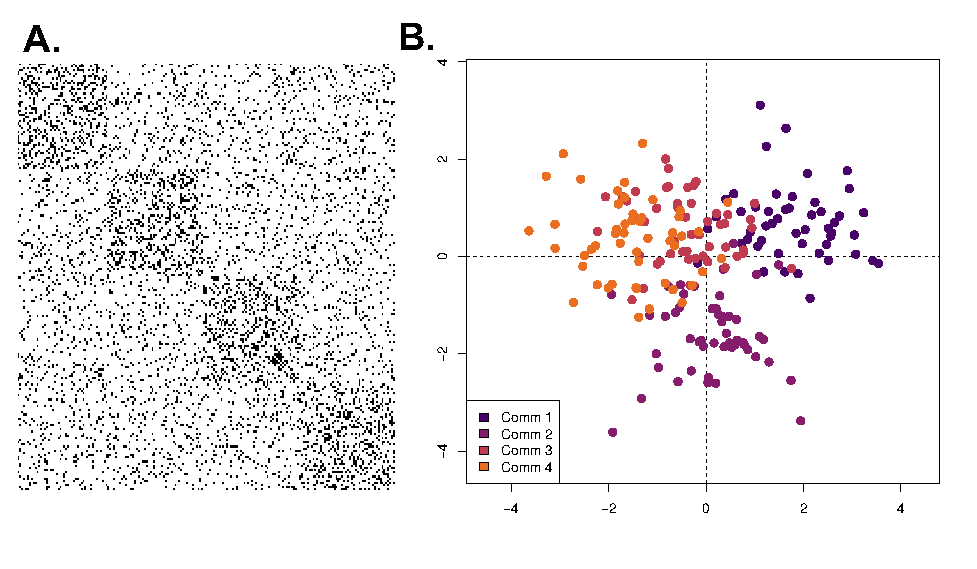
\includegraphics[width=0.5\textwidth]{SyntheticFig.pdf}
\caption{{\bf Synthetic Example.} We generated a synthetic network with $N=200$ nodes, $K=4$ communities and an 8-dimensional multivariate Gaussian for each community. {\bf A.} A visualization of the adjacency matrix for this network where a black dot indicates an edge. We observe that there is an assortative block structure (blocks on the diagonal), but there are also many 'noisy' edges between communities making the true community structure with only a stochastic block model a bit harder to detect. {\bf B.} We performed PCA on the $N \times p$ dimensional attribute array and plotted each of the $N$ nodes in two dimensions. Points are colored by their true community assignments, ${\bf z}$. Clustering the nodes according to only connectivity, only attributes, and with the attributed SBM, we quantified the partition accuracy with normalized mutual information. This gave results $\text{NMI}({\bf z},\{{\bf z}^{\text{connectivity}}, {\bf z}^{\text{attributes}},{\bf z}^{\text{attribute sbm}}\})=\{0.65,0.68,0.83\}$.}
\label{fig:AttFig2}
\end{center}
\end{figure}

\indent To assess how well the attribute SBM approach performed in successfully assigning nodes to communities, we compared the results obtained from our model to clustering results obtained either only clustering the nodes based on connectivity, and to results of clustering nodes based only on their attribute information. We quantify the correctness of the partition with normalized mutual information (NMI) \cite{commdeccompare}. Letting ${\bf z}$ denote the true node-to-community assignments, then ${\bf z}^{\text{connectivity}}$, ${\bf z}^{\text{attributes}}$, and ${\bf z}^{\text{attribute sbm}}$ denote the partition of the nodes according to only the network connectivity only, attributes only, and with the attributed SBM. To cluster the network only according to connectivity, we fit a stochastic block model with 4 blocks. To cluster nodes with only attributes, we performed $k$-means clustering on only the attributes. Computing the NMI between ${\bf z}$ and each of these 3 cases, or $\text{NMI}({\bf z},\{{\bf z}^{\text{connectivity}}, {\bf z}^{\text{attributes}},{\bf z}^{\text{attribute sbm}}\})=\{0.65,0.68,0.83\}$. These results show that by combining both sources of information, there is an improvement in the ability to correctly identify communities. To further probe this idea, we sought to empirically look closer at the so-called 'detectability limit'. Generally, detectability refers to the difficulty of correctly identifying clusters in data. Multiple works \cite{decelle2011inference,taylor2015enhanced} have explored these limits in stochastic block models observing the sharp phase transition that occurs in accuracy as soon as within-community probability ($p_{in}$)  is sufficiently larger than the between-community probability ($p_{out}$). 

\indent Based on the results of the synthetic experiments in Figure \ref{fig:AttFig2} where the attributes combined with connectivity lead to a more accurate partitioning of the nodes, we hypothesized that augmenting the network connectivity with attributes could somehow move this detectability limit. In Figure \ref{Att:Detect}, we explored how generating networks from a stochastic block model with varying ratios between $p_{in}$ and $p_{out}$ combined with the attributes used in Figure 2 would affect the accuracy of the node-to-community partition. To do this, we considered values of $p_{in}$ between 0.05 and 0.3 in increments of 0.05. For each of these $p_{in}$ values, we found the corresponding value of $p_{out}$ such that the mean degree was 20. Fixing the mean degree allows for direct comparison of how the within-to-between community probabilities influence the detection of correct communities. For each of these $p_{in}$ and $p_{out}$ combinations, we generated 10 different networks using a stochastic block model. In figure 3 we plot the NMI between the true partition, ${\bf z}$ and the partitions using only the connectivity with the regular SBM ${\bf z}^{\text{connectivity}}$ and the attributed SBM ${\bf z}^{\text{attribute sbm}}$. These results are plotted in blue and pink, respectively. The shaded region around the points indicates standard deviation. 

\subsection{Detectability analysis}
\begin{figure}[h!]
\begin{center}
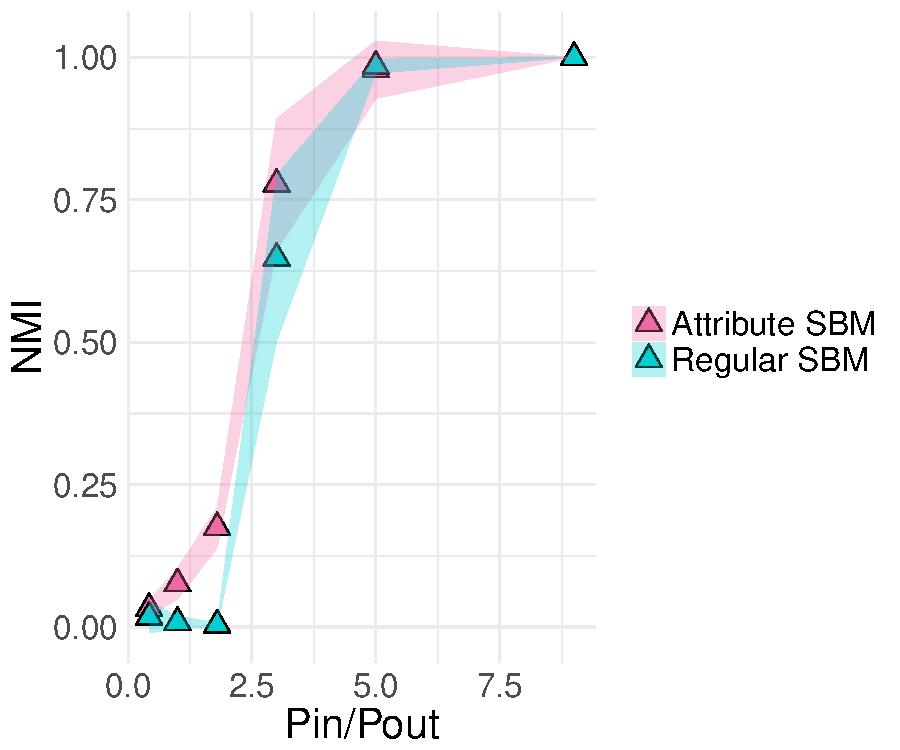
\includegraphics[width=0.4\textwidth]{DetectExp.pdf}
\caption{{\bf Detectability Analysis in Synthetic Example.} To understand how attribute information can be combined with connectivity to assign nodes to communities accurately, we generated synthetic networks for within-probabilities of $p_{in}$ between 0.05 and 0.3 with corresponding $p_{out}$ or between-community probabilities such that the mean degree of the network was 20. For each of these synthetic networks, we used the attributes from the analysis in figure 2 to fit the attributed SBM. Here, we plot the correctness of the node-to-community assignment with normalized mutual information using the partition obtained from regular SBM (blue) and the partition under the attributed SBM model fit (pink). For each combination of $p_{in}$ and $p_{out}$, we generated 10 networks and hence the bands around the points denote standard deviation. Incorporating attributes with the attributes stochastic block model shifts the detectability limit slightly to the left. }
\label{Att:Detect}
\end{center}
\end{figure}

We see that while both inference approaches undergo a phase transition at a similar ratio of $p_{in}/p_{out}=3$, we notice that the curve for the attribute SBM model is slightly shifted to the left suggesting that the extra attribute information does positively impact the ability to correctly identify communities. Future work could focus on understanding detectability questions in relation to the parameters for the underlying multivariate Gaussian distributions parametrizing each community. For example, how does the difference in means between a pair of communities shift the detectability curve?

\section{Using the fitted attributed SBM for link prediction and collaborative filtering}
One of the benefits of a generative network model is that it can be applied to prediction tasks. Most notably, in the absence of one source of information about a node (connectivity or attributes), the model can be used to predict the complementary information source (attributes or connectivity, respectively). By fitting an attributed SBM, obtained successful performance in two fundamental network prediction tasks, link prediction and collaborative filtering. 

\subsection{Link Prediction Methods}
In the link prediction problem, when given two node stubs, the objective is to determine whether a link exists between them. Since we are modeling connectivity with a stochastic block model, we can predict links using the learned parameters.  In particular, we highlight how this task can be performed using just the attribute information of the node stubs of interest. In the experiments to follow, we compare to 3 commonly-used link prediction methods. In all of these methods, a score is computed for all pairs of edge candidates and ultimately the top $x$ set of edges with highest weights are kept (where $x$ is some user-defined parameter). Let $m$ and $n$ be a pair of nodes and $\Gamma(m)$ denote the set of neighbors for a node $m$. Then, under the following 3 common  link prediction methods \cite{linkPredReview}, we can calculate the score of the potential link as, $\text{Score}(m,n)$.

{\bf Jaccard}: $\text{Score}(m,n)= \frac{\Gamma(m) \cap \Gamma(n)}{\Gamma(m)\cup \Gamma(n)}$

{\bf Adamic Adar}: $\text{Score}(m,n)=\sum_{c \in \Gamma(m) \cap \Gamma(n)}\frac{1}{\log |\Gamma(c)|}$

{\bf Preferential Attachment}: $\text{Score}(m,n)=|\Gamma(m)|\times |\Gamma(n)|$\\

For the link prediction tasks shown in figures 5 and 9, we performed a link prediction task by sampling pairs of nodes and utilizing the complementary source of attribute information. We sampled 10 different sets of 50 pairs of nodes. In each sample, 25 of the node pairs were those having an edge in the original network and 25 were pairs with no edge. For each of the 50 edges in each sample, we sought to predict whether an edge existed between the corresponding node pair in a leave one out manner. To do this, for each edge we fit the attributed SBM to the network with the pair of nodes (stubs) associated with the edge removed. We then use the nearest neighbor in attribute space of each stub as the the input to each of the 3 baseline community detection methods (Jaccard, Adamic Adar, and Preferential Attatchment). To use our attributed SBM in this link prediction task, we also consider the most commonly observed community among the 3 nearest neighbors for the stubs of the edge of interest. Again, using the nearest neighbors, which we denote by $n$ and $m$ of the stubs, then we define the link prediction score for the edge as $\theta_{z_{n},z_{m}}$, or the probability that an edge exists between nodes $n$ and $m$ according to the fitted model. After generating 10 samples of 50 edge pairs, this results in 500 total edge scores. Since we know the ground truth of whether or not these edges actually exist from the original network, we can construct an ROC curve for each method. From these curves we can plot area under the curve (AUC) to quantify the quality of the link prediction result. Using the attributed SBM is a way to incorporate community information into the link prediction problem which has previously shown to be effective \cite{linkComm}.

\subsection{Collaborative Filtering Methods}
Conversely, the collaborative filtering problem seeks to predict a node's attributes based on its similarity to its neighbors. For some node of interest, we can use our fitted attributed SBM model to predict a node's attributes, given only the information about its connectivity. Formally, for node $i$, we seek to predict ${\bf x}_{i}$. In the following experiments, we compare our results to two common collaborative filtering approaches \cite{collabFilterReview}. Let $\mathcal{N}^{k}(m)$ be the set of $k$-nearest neighbors in the network for node $m$. Let $\hat{{\bf x}_{i}}$ be the predicted attribute vector for node $i$ and $s_{ij}$ be a similarity measure between nodes $i$ and $j$. 

{\bf Neighborhood Avg}: $\hat{{\bf x}_{i}}= \frac{1}{|\mathcal{N}^{k}(i)|}\sum_{j \in \mathcal{N}^{k}(i)} {\bf x}_{j}$

{\bf Weighted Neighborhood Avg}: $\hat{{\bf x}_{i}}=\frac{1}{\sum_{j in \mathcal{N}^{k}(i)}s_{ij}}\sum_{j \in \mathcal{N}^{k}(i)}s_{ij}{\bf x}_{j}$

In collaborative filtering experiments, the objective is to predict the vector of attributes for each node. In our experiments, we used leave-one-out validation to predict the attribute vector for each node. That is, for each node in the network, we created a single node test set. The training set, was then the rest of the network with the node to predict removed. For this single test set node, we identified neighbors it connects to in only connectivity space within the training set. For standard collaborative filtering approaches (Neighborhood average and weighted neighborhood average), the predicted attribute for the test set node is then the specified averaging of the neighbors. To use our model for this task, we first fit the attributed SBM model to the training set. Similar to the standard link prediction approaches, we identify the nearest neighbors for our test node in connectivity space within the training set. We then predict the community membership of our test node to be the most-frequently observed community among its neighbors. Using this community assignment, $c$, we then predict the attribute vector for our test node to be ${\bf \mu}_{c}$, or the mean vector that was learned to describe community $c$. The results of collaborative filtering experiments for the microbiome and protein network examples are shown in figures 6 and 10. For a node $i$ and its associated vector of attributes, ${\bf x}_{i}$ we quantify the accuracy of the predicted attribute vector, $\hat{{\bf x}_{i}}$ with a a relative error measure, $\mathcal{E}$, such that 
\begin{equation}
\mathcal{E}=\frac{||\hat{\bf{x}}_{i}-{\bf x}_{i}||_{2}}{||{\bf x}_{i}||_{2}}.
\end{equation}

Similar to the success of integrating community information for link prediction, an collaborative filtering tasks have previously shown success from the integration of network community structure \cite{collabComm}. 

\section{Applications in Biological Networks}
We evaluate the potential to combine similarity or relational information between a set of entities for application in biological data. Whether that be networks of proteins, genes, or bacterial species with extra experimental data. Our application of this model to biological problems provides a framework to predict attribute or connectivity information about a new observation.  Note that we do not intend to suggest any new biological insights, but rather that we can combine two sources of information for prediction tasks and alternative definitions of what constitutes a community in the data. Applying the attributed stochastic block model to integrate connectivity and attribute data provides a way to find a partition that takes into account two different sources of information, or a method to predict one source of information (connectivity, attributes) in the absence of the other (attributes, connectivity). 

\subsection{Microbiome Subject Similarity Results}

\subsubsection{Motivation}

In the analysis of biological data, it is often useful to cluster subjects based on a set of their measured biological features and to then determine what makes each of the subgroups different. One type of biological data gaining much attention in recent years is metagenomic sequencing data, used to profile the composition of a microbiome. We refer to this as the 'metagenomic profile' and each feature is a count for each bacterial species, also known as operational taxonomic unit (OTU). Lahti et al. conducted a study among subjects across a variety of ethnicities, body mass (BMI) classifications, and age groups to understand differences in the intestinal microbiota \cite{microbiomedata}. Using metagenomic sequencing, the counts for 130 OTUs were provided for each subject. We created an experiment to test our model by seeing if we could overlay a similarity network between subjects with the individual OTU count vectors for each subject. 

\subsubsection{Pre-Processing}
The data were downloaded from \url{http://datadryad.org/resource/doi:10.5061/dryad.pk75d}. We extracted a subset of the subjects from Eastern Europe,Southern Europe,Scandinavia, and the United States. Using only these subjects, a between-subject similarity network was constructed between the 121 individuals who had a BMI measurement. This resulted in a network of 121 nodes, where each edge is the pearson correlation between their microbial compositions. We then removed all edges in the network with weight (correlation) <0.7. Note that our attributed SBM does not allow for edge weights, so as input of this network into the model, we simply ignored the edge weights. 

\subsubsection{Constructing Node Attributes}
Since each node had a 130-dimensional vector of attributes (counts), we used this information to create a lower-dimensional attribute vector for each node by performing PCA and then representing each node with the first 5 principal components. Each dimension of this new attribute vector was then centered and scaled and has an approximately gaussian distribution. 

We first visualized the differences in partitions obtained according to the classic and attributed stochastic block models in figure 4A-B, respectively. In both networks, nodes are colored by their community assignment. Using the classic stochastic block model and the model selection criteron described in \cite{dudin}, 7 blocks were identified. With the attributed stochastic block model, 6 blocks were identified. While we do not have ground truth labels on the nodes, it is visually apparent that adding the attributes to the inference problem helps to 'clean up' the partition. For example, in figure 4A there is mixing between the dark and lighter purple communities in the upper left of the network. In figure 4B, this mixing was reduced by assigning all of the nodes in the general region to the lighter purple community. 

\begin{figure}[h!]
\begin{center}
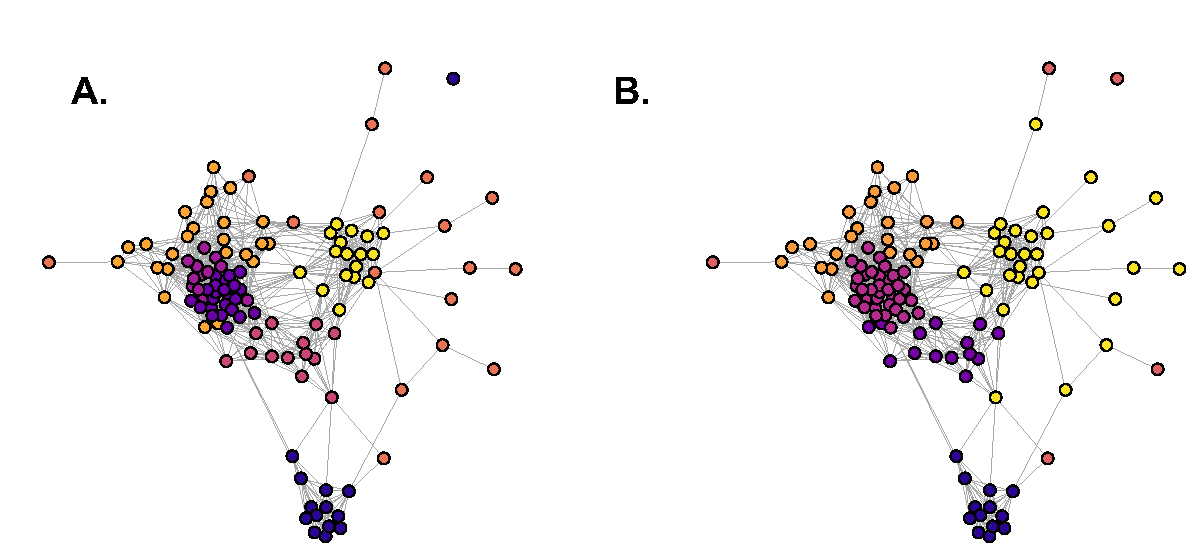
\includegraphics[width=0.7\textwidth]{MicrobiomeNets_Dec12.pdf}
\caption{{\bf Microbiome subject similarity network:} A visualization of the 121 node microbiome subject similarity network with nodes colored by the partition using the classic ({\bf A.}) and attributed ({\bf B.}) stochastic block model. {\bf A.} Fitting the classic stochastic block model to the network, 7 communities were identified. {\bf B.} Fitting the attributed stochastic block model to the network with the attributes being the first 5 principle components of each subject's OTU count vector (metagenomic profile), 6 communities were identified. Incorporating attributes in inferring this partition removed some of the noise in the partition on the network, specifically in the mixed purple community in the left of {\bf A.}}
\end{center}
\end{figure}

\subsubsection{Link Prediction Experiments}
We performed link prediction on the microbiome subject similarity network as described in section 4.1. The associated ROC curves are plotted in figure 5. All four methods have satisfactory performance with the attributed stochastic block model giving the best results. The AUC values for the attributed sbm, Jaccard, Adamic Adar, and preferential attachment are 0.71, 0.69, 0.69, and 0.62, respectively. 
 
\begin{figure}
\begin{center}
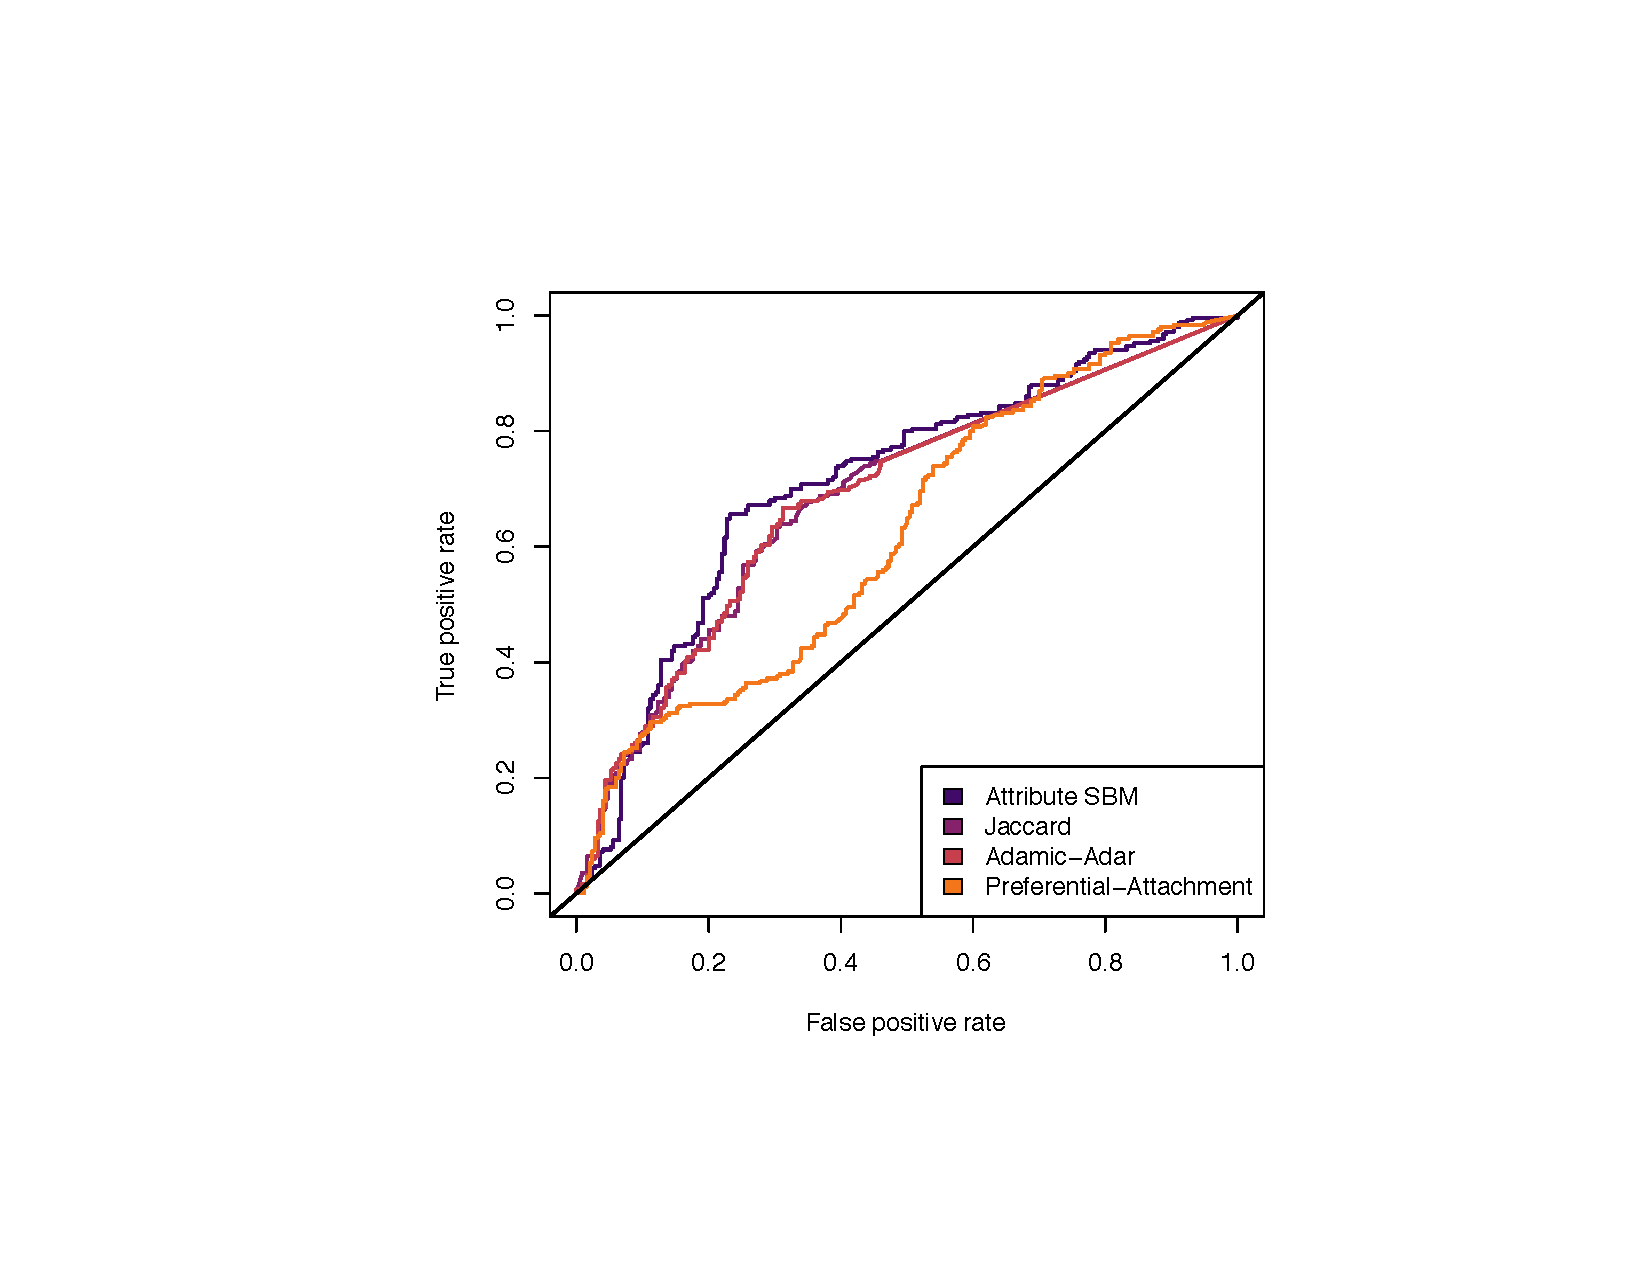
\includegraphics[width=0.6\textwidth]{ROC_Microbiome.pdf}
\caption{{\bf Link Prediction on the microbiome subject similarity network:} The results for link prediction on the microbiome subject similarity network for the attributed SBM, Jaccard, Adamic-Adar and preferential attachment methods. The corresponding AUC values for these methods, respectively are, 0.71, 0.69, 0.69, and 0.62.}
\end{center}
\end{figure}

\subsubsection{Collaborative Filtering Experiments}
We performed the collaborative filtering experiments on the microbiome subject similarity network in the manner described in section 4.2 to predict the 5-dimensional attribute vector for each node. The box plots indicate the distribution of relative errors over the 121 nodes for the attribute SBM (blue), neighbor average (pink) and weighted neighbor average (orange). While the attributed SBM plotted has a similar distribution of relative errors with the standard collaborative filtering methods, the mean is slightly lower, at 0.21, compared to 0.26 and 0.27 in the neighbor average and weighted neighbor average, respectively.
\begin{figure}[h!]
\begin{center}
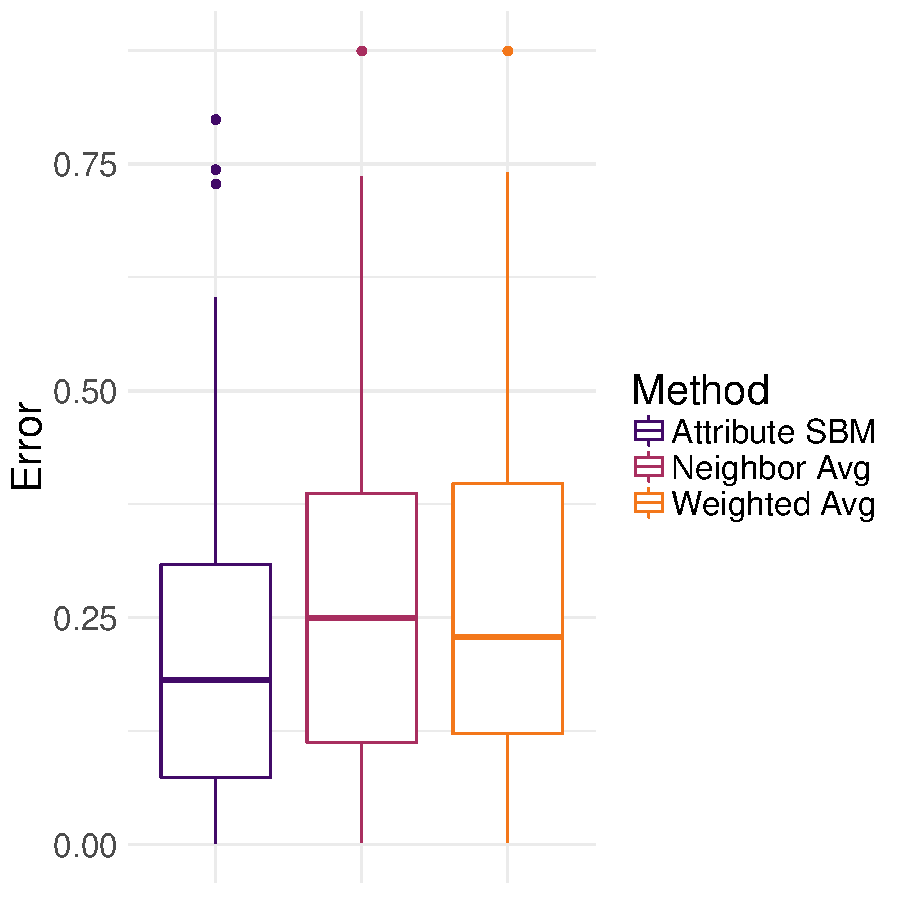
\includegraphics[width=0.5\textwidth]{CollabFilterMicro.pdf}
\caption{{\bf Collaborative Filtering Accuracy in Microbiome Subject Similarity Network}: For each of the 121 nodes, we fit a model to the remaining 120 node network and given the node's closest  neighbors (based on network connectivity) sought to predict its 5-dimensional attribute vector. The reported error is the relative error $\mathcal{E}$ between the difference between the true attribute vector (${\bf x}_{i}$) and its predicted attribute vector (${\hat{\bf x}}_{i}$). The mean error in ${\bf x}_{i}$ is 0.21, as opposed to the neighbor average and weighted neighbor averages, having errors of 0.26 and 0.27, respectively. }
\end{center}
\end{figure}

\subsection{Protein Interaction Network Results}
We also apply our attributed SBM approach to the protein interaction network presented in \cite{bonacci}. This network represents interactions between proteins, predicted from the literature. Associated with each each node (protein), is a classification of one of 6 experimental modifications observed from the exposure of cancer cells to a chemotherapeutic drug. While communities in this network should reflect functional relatedness among proteins (i.e. similar biological functions, in general), we also expect that members of a community should share similarities in the observed modification type. Also associated with each of the 6 modification types is whether that particular type of modification became either more or less prominent after treatment with the drug. Since we have two types of labels associated with these nodes, we also sought to explore how these two labeling schemes (6 class vs. 2 class) aligned with the communities returned by the algorithm. 

\begin{figure}[h!]
\begin{center}
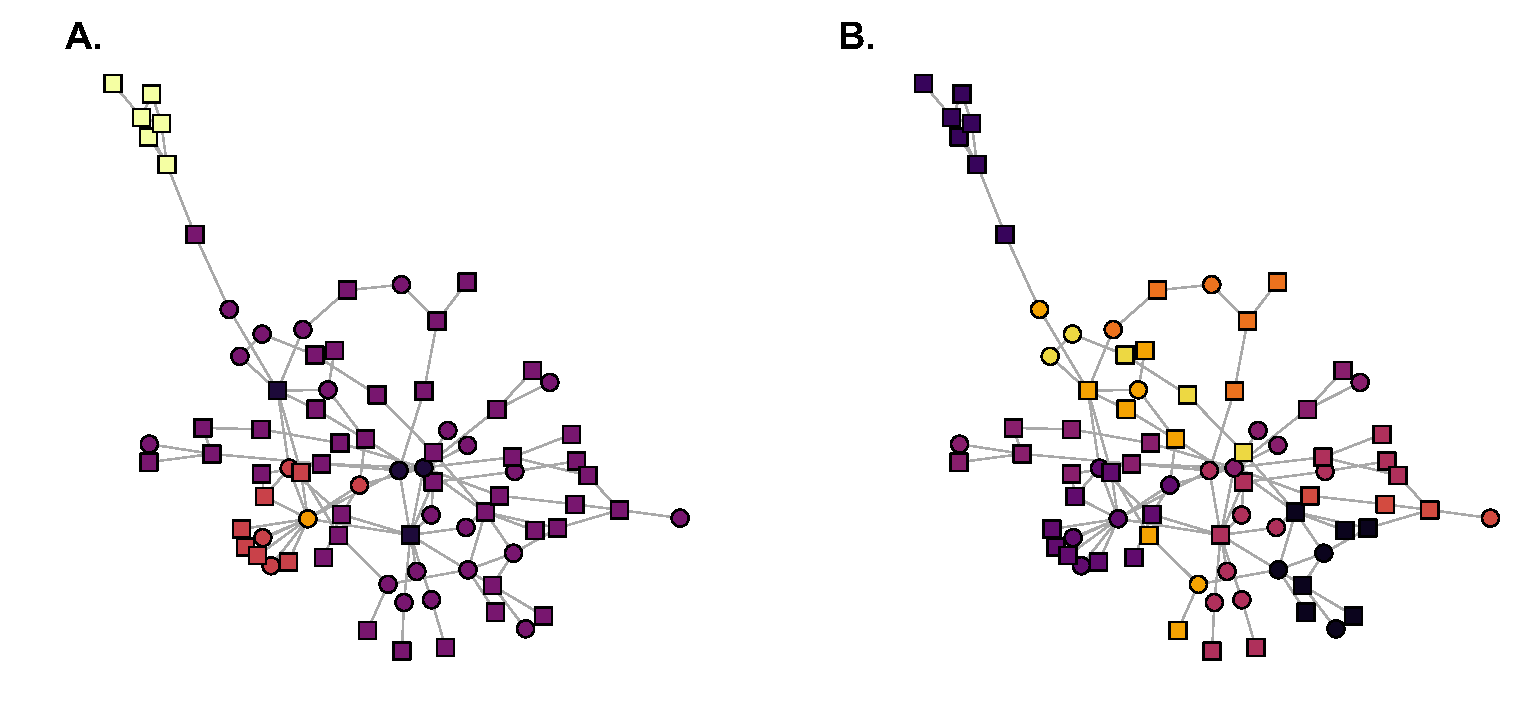
\includegraphics[width=0.7\textwidth]{ProteinNet_Dec12.pdf}
\caption{{\bf Protein interaction network.} We visualize the 82 node protein interaction network under the classic stochastic block model {\bf A.} and the attributed stochastic block model {\bf B.} In both networks, nodes are colored by their community assignment and the node shape indicates whether the modification status increased (square) or decreased. {\bf A.} Nodes colored according to the community partition under the stochastic block model. Nodes are assigned to one of five communities. {\bf B.} Nodes are colored to the community partition under one of nine communities.}
\end{center}
\end{figure}

\subsubsection{Data Pre-Processing} We downloaded the unweighted protein interaction network data and the modification information from the supplement of \cite{bonacci}. We removed 13 nodes that were not connected to the giant component of the network and considered only the 82 node giant connected component.

\subsubsection{Constructing Node Attributes}
As previously described, each node is classified with 1 of 6 possible modification type. For each node, we created an attribute vector that captured the modification types of its neighbors. To do this, we considered the 4th order neighborhood of each node. That is, for each node, we collected its neighbors who were four hops or less away in the network. Then to define the value for attribute $c$ of node $i$, or $x_{ic}$, we counted the number of fourth order neighbors of node $i$ with label $c$. After defining these attributes across all nodes, for each of the 6 classes, we centered and scaled each attribute across all of the nodes to have mean 0 and unit variance. 

Figure 7A-B show the results of fitting a classic SBM and attributed SBM, respectively.  The 6 possible modifications exist for 3 biological processes that can either increase or decrease. The node shape reflects whether the experimental modification for a node increased (square) or decreased (circle) after treatment with the chemotherapeutic agent. Again by fitting an SBM with the model selection criterion in \cite{dudin}, 5 communities were identified. With our attributed SBM, 9 communities were identified. Note that using the attributed SBM created more communities in that it split up the purple core community under the classic SBM into more small communities. The implications of this new partition are explored with an entropy calculation based on the biological classifications of the protein in Figure \ref{entropyFig}.
 \begin{figure}[h!]
\begin{center}
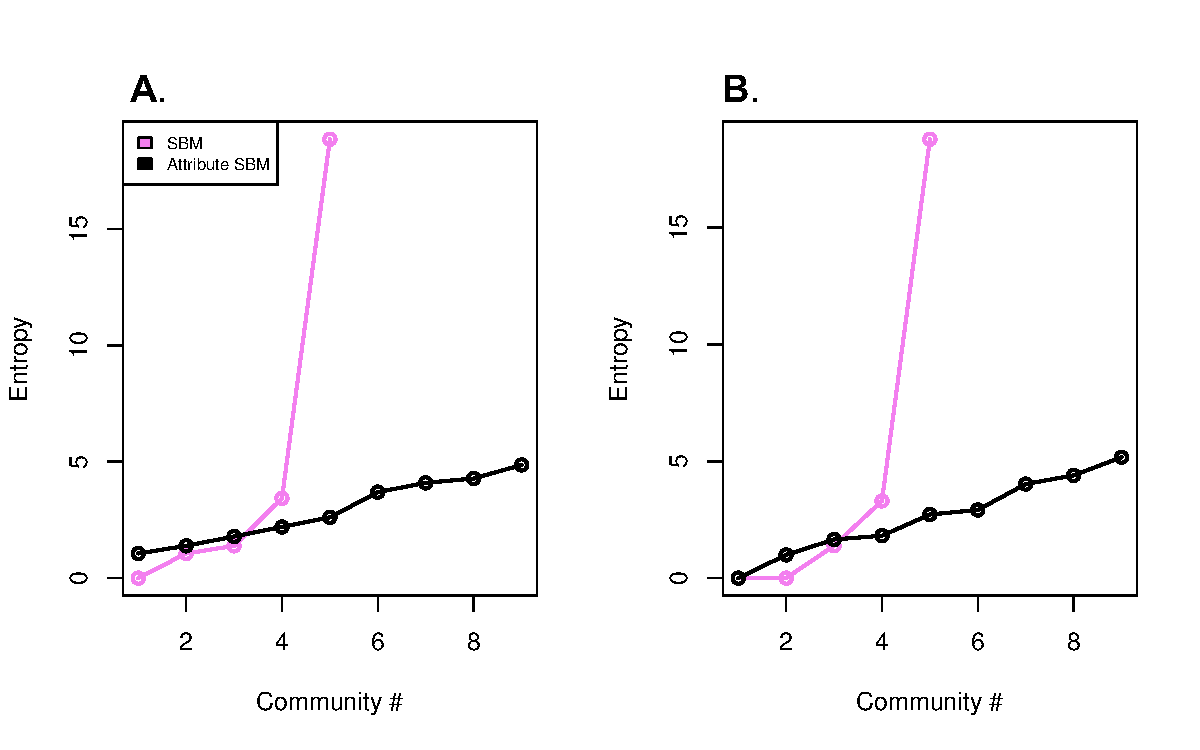
\includegraphics[width=0.8\textwidth]{EntropyCalc_6Classleft_2classright.pdf}
\caption{{\bf Community entropies in the protein interaction network.} We studied the entropy of the 2 class and 6 class classifications of the nodes in {\bf A.} and {\bf B.}, respectively under the classic SBM (black) and attributed SBM (purple) partitions. For ${\bf A.-B.}$ the horizontal axis denotes the community index for the particular partition. Nodes belonged to 1 of 5 communities under the classic SBM and belong to 1 of 9 communities with the attributed SBM. Incorporating attributes under both classifications succeeds in breaking up a high entropy community (5) from the classic SBM partition to lower entropy communities in the attributed SBM partition. }
\label{entropyFig}
\end{center}
\end{figure}

Using the partition of the nodes under the classic and attributed stochastic block models, we sought to use the two different classifications of the nodes (6 class modification type and 2 class increase/decrease) to compute entropy of labels within communities. The expectation is that by incorporating attribute information that is related to the functional protein information into the community detection problem, we should see a decrease in the entropy over the classification labels in communities. In figure 8A-B, we plot the entropy for the 2 class and 6 class node classifications, respectively. We define ${\bf E}_{c}$, the entropy for community $c$ as,

\begin{equation}
{\bf E}_{c}=-\sum_{k} p_{k}\log(p_{k}).
\end{equation}.

Here, $k$ is indexing the unique classifications found in community $c$ and $p_{k}$ is the probability that a node in community $c$ belonged to classification $k$ in community $c$. In these plots the black and purple curves correspond to the fits of the classic and attribute SBM fits, respectively. Using both types of node classifications to compute these entropy quantities, we see that the attribute SBM succeeds in breaking up one high entropy community (5) from the classic SBM partition into lower entropy communities. 

\subsubsection{Link prediction experiments}
We performed link prediction on the protein interaction network using the procedure described in section 4.1. Given that this protein network is sparse, none of the link prediction methods performed particularly well. The AUC values for the attributed SBM, jaccard, adamic adar and preferential attachment were 0.61, 0.58, 0.58, and 0.54, respectively. The associated ROC curves are shown in figure 9.  

\begin{figure}[h!]
\begin{center}
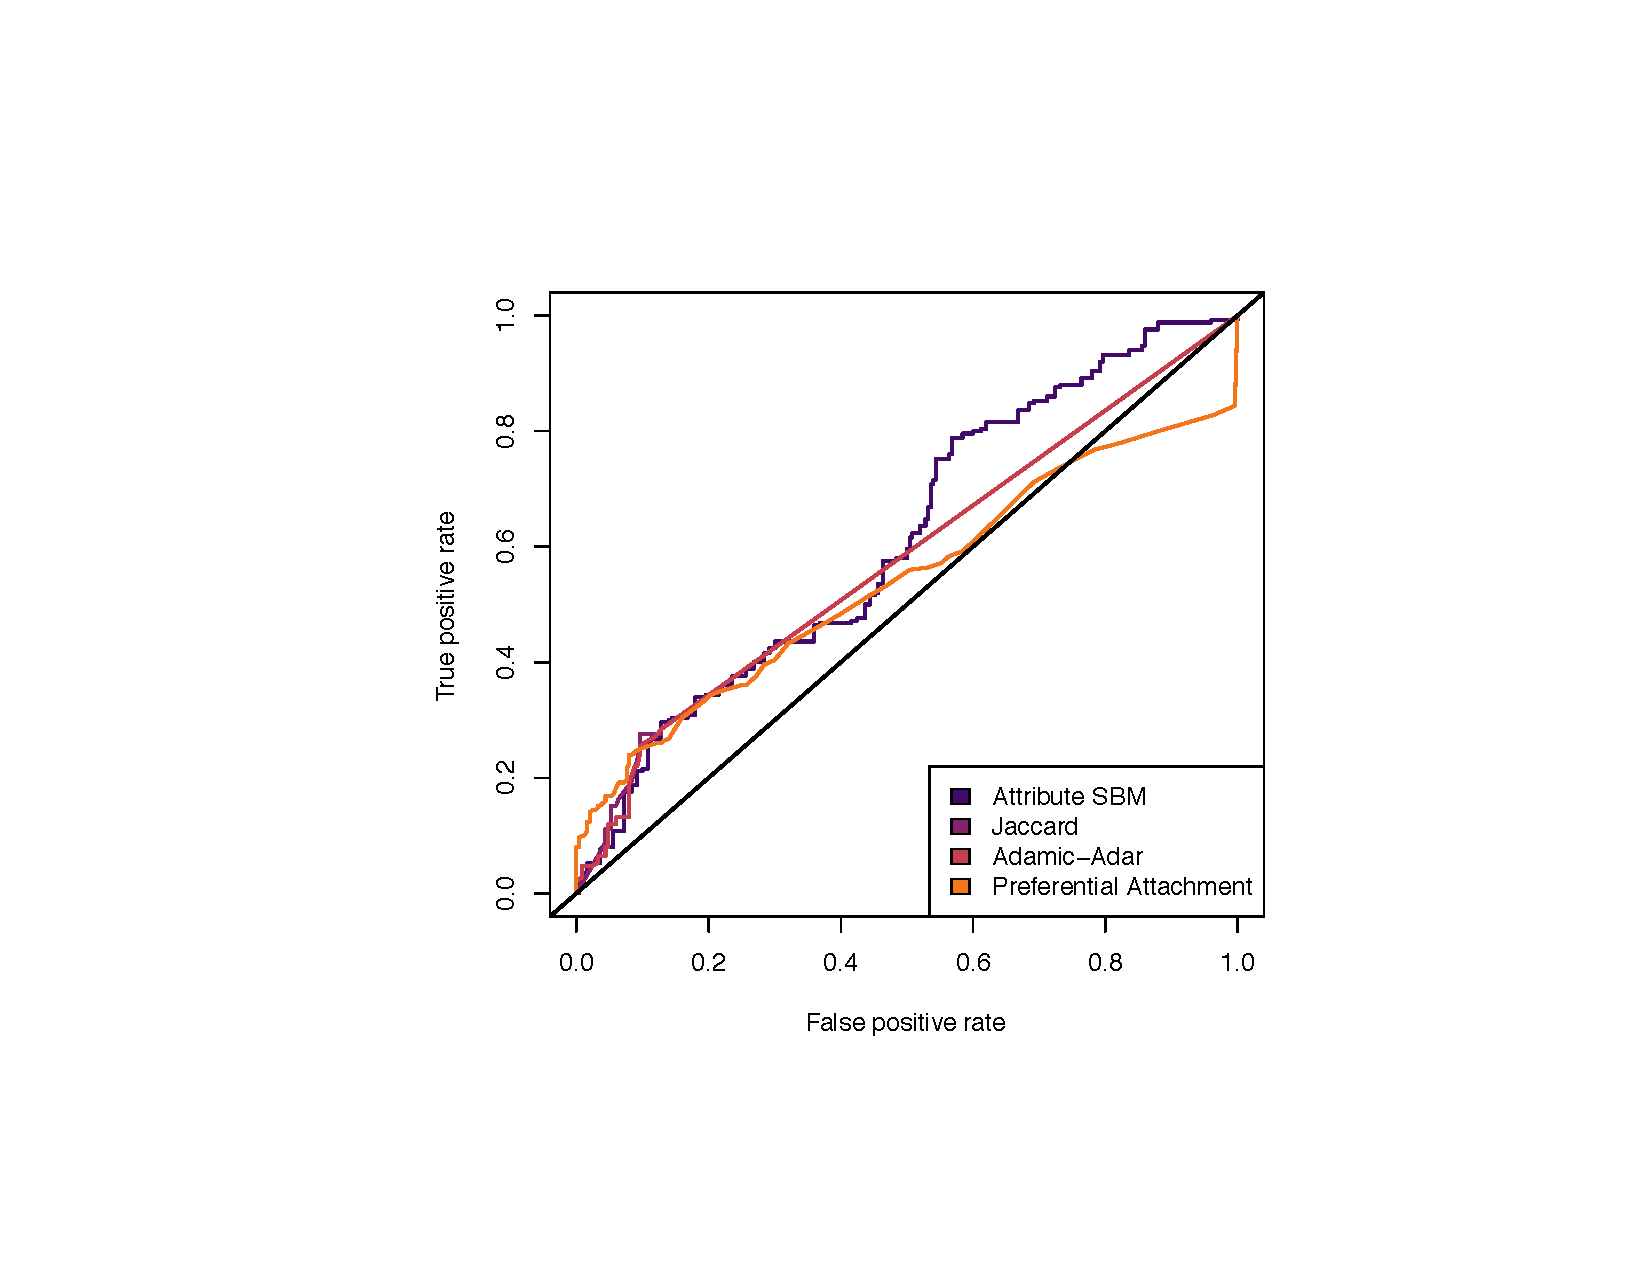
\includegraphics[width=0.6\textwidth]{ROC_Protein.pdf}
\caption{{\bf Link Prediction in the protein interaction network}. Performing link prediction using the attributed SBM, Jaccard, Adamic Adar, and preferential attachment. The corresponding AUC curves for these methods were 0.61, 0.58, 0.58, and 0.51, respectively.}
\end{center}
\end{figure}

\subsubsection{Collaborative filtering experiments}
Collaborative filtering was performed using the method described in section 4.2. Note that unlike the microbiome sample similarity network, the edges in this network are unweighted and hence the neighbor average and weighted neighbor average methods produce the same result. We note that performing collaborative filtering with the attributed stochastic block model results in a lower mean error of 0.21 compared to that of 0.48 when using the neighbor average. Similar to figure 5, the box plots in Figure \ref{collabprotein} represent the distribution of errors across each of the 82 nodes.

\begin{figure}[h!]
\begin{center}
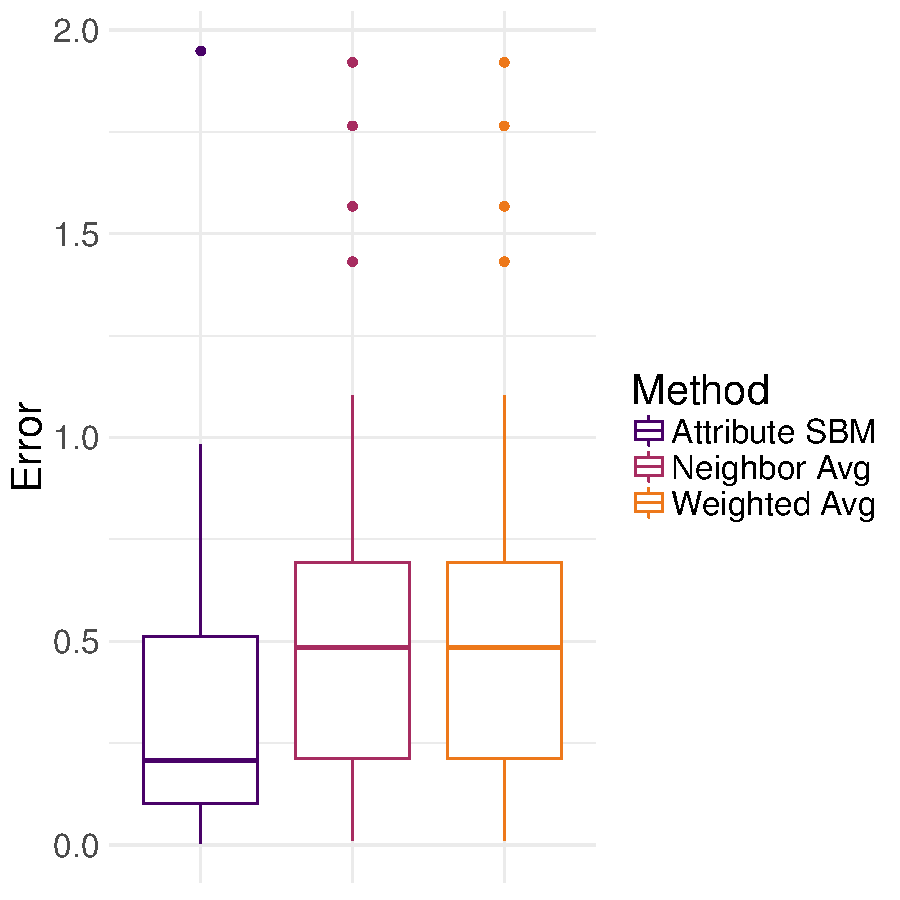
\includegraphics[width=0.5\textwidth]{CollabProtein.pdf}
\caption{{\bf Collaborative filtering in the protein interaction network}. For each of the 82 nodes, we fit a model to the remaining 81 node network and given the node's closest  neighbors (based on network connectivity) sought to predict its 6-dimensional attribute vector. The reported error is the relative error $\mathcal{E}$ between the difference between the true attribute vector (${\bf x}_{i}$) and its predicted attribute vector (${\hat{\bf x}}_{i}$). The mean error in ${\bf x}_{i}$ using the attributed SBM is 0.21, as opposed to the neighbor average error where it is 0.48. }
\label{collabprotein}
\end{center}
\end{figure}

\section{Conclusion and Future Work}
In this paper, we defined an attributed stochastic block model, where a node's community assignment determines its connectivity and its attribute vector. Our model builds on previous work with attributed stochastic block models because it can handle multiple continuous attributes. The continuous attributes are modeled by a Gaussian mixture model, where the assumption is that the attributes for members for each community are parameterized by a unique multivariate Gaussian. Since community detection results are often difficult to validate due to the lack of unlabeled network data, or definition of what a correct partition means, we quantified the ability of the fitted attributed stochastic block model to represent a particular network by performing link prediction and collaborative filtering tasks. Applying link prediction and collaborative filtering to two biological networks, we observed that the attributed SBM is useful for these applications.

Future work could extend the model to handle a combination of multiple discrete and continuous attributes. Further, while the inference or understanding of fitting a stochastic block model to weighted networks is not well understood, figuring out how to integrate edge weights and attributes in determining community structure could be useful. Finally, we briefly discussed a detectability problem in figure 3. Interesting future work could aim to characterize the properties of the attributes and connectivity and how they relate to effective identification of community structure.

Networks used across fields are becoming increasingly complex, often with multiple sources of information to integrate in order to make a conclusion for the data. Our approach to an attributed SBM advances the understanding of how to jointly consider attribute and connectivity information in a probabilistic framework.  

\chapter{Testing the Alignment of Node Attributes with Network Structure}
Attributed network data is becoming increasingly common across fields, as we are often equipped with information about nodes in addition to their pairwise connectivity. This extra information can manifest as a single value or classification for the nodes, or as multidimensional vector of features. Recently developed methods that seek to extend community detection approaches to attributed networks have explored how to most effectively combine connectivity and attribute information for quality identification of communities. These methods often rely on some assumption of the dependency relationships between attributes and connectivity. In this work, we seek to develop a statistical test to assess whether node attributes align with network connectivity. The objective is to quantitatively evaluate whether nodes with similar connectivity patterns also have similar attributes. To address this problem, we will use a node sampling and label propagation approach. We apply our method to several synthetic examples that explore how network structure and attribute characteristics effect the empirical $p$-value computed by our method. Finally, we apply the test to a network generated from a single cell mass cytometry dataset and show that our test can identify markers associated with particular inferred cellular phenotypes. 

\section{Introduction}

Community detection in networks is a common pursuit that seeks to partition the network's nodes into sets of structurally coherent groups, where members of a group of \emph{community} have strong similarity in connectivity patterns \cite{muchacommunity,fortu2,shaicase}. While the identification of communities based solely on the network's adjacency matrix is straight forward, the implications of having extra information about the network nodes and how to integrate that into the community detection problem is not well-understood. We refer to a \emph{structural community} as a community identified according to only the adjacency matrix, while an \emph{attribute community} can be thought of as a community identified using the attribute information. Recently, there have been numerous approaches extending common community detection techniques to attributed networks \cite{hric,peel2017ground,ilouvain,cesna,clauset,perozziAttribute}. While each of these methods provide extensions to different community detection approaches, they also differ in their assumption about the dependence relationships between the attributes and connectivity. On one hand, it seems reasonable to assume that members of a structural community should be highly similar in attribute space seems like a valid assumption. However, work by Clauset \emph{et al.} \cite{clauset} and Peel \emph{et al.,} \cite{peel2017ground} have provided examples of when this assumption could be invalid. In this work, we seek to develop a test that returns a statistic providing insight into how closely the node attributes correlate with connectivity patterns. Our test is based on label propagation and ultimately returns an empirical $p$-value that can be interpreted as the significance of the relationship between network connectivity and node attributes. We validate that the empirical $p$-value is meaningful with several synthetic examples and on a network representation of a single-cell mass cytometry dataset. 

This paper is organized as follows: First, we will describe the latest advances in attributed community detection. Next, we will describe our method and validate the quality of the computed empirical $p$-value on synthetic examples and on a single cell mass cytometry dataset. 

\subsection{Attributed Network Community Detection Methods}
There are numerous classes of community detection methods, such as, probabilistic \cite{sbmOrig,bigclam}, quality function maximization\cite{newmanmodularity}, and higher-order motif-based clustering \cite{benson}. Most of these approaches have consisted of some work for the most appropriate adaptation to attributed networks. Here we will discuss extensions to probabilistic and quality function maximization approaches. Note that this section has a very similar discussion to Chapter 4.1, but it is more closely adapted to the work discussed here.

\subsubsection{Probabilistic approaches}
Probabilistic community detection methods seek to model network edges based on some rule that takes into account the community structures. One a model is its parameters are optimized through likelihood optimization and are considered optimal if a sample generated from the learned model aligns closely to the true underlying network. Two common approaches are the stochastic block model (SBM) \cite{sbmOrig} and the affiliation model \cite{bigclam}. 

The assumption of the stochastic block model is that nodes within a community are connected to nodes within and between communities in a characteristic way. Moreover, the objective in the fitting and parameter inference of a stochastic block model in a network with $K$ communities is to learn the node-to-community assignments and the within and between community connection probabilities that maximize the model likelihood. The stochastic block model has been extensively studied in the literature and has at least three attempts to be extended to attributed networks \cite{hric}, \cite{peel2017ground}, \cite{clauset}. First, Clauset \emph{et al.}, modified the traditional stochastic block model likelihood to incorporate a piece of metadata \cite{clauset}. Related to this work, Peel \emph{et al.}, proposed the neoSBM \cite{peel2017ground}, which developed a permutation-based test to assess the relatedness of attributes and connectivity and incorporated the information only to the extent to which they were aligned. Next, Hric \emph{et al.}, constructed a joint stochastic block model for both the attributes and metadata through a nonparametric, bayesian framework \cite{hric}. They assessed the alignment of the attributes with the connectivity based on their application in link prediction tasks. 

The affiliation model assumes that nodes can be affiliated to multiple communities to varying extents \cite{bigclam}. Moreover, the edges between a pair of nodes is based on their similarity in community affiliations. A useful method for integrating multidimensional vectors of binary attributes was introduced by Yang \emph{et al.} in a method called CESNA \cite{cesna}, which modifies the affiliation model likelihood to incorporate this information. This is achieved by allowing the attributes and connectivity information to be modeled as conditionally independent, giving the node-to-community affiliations and feature importance weights for the attributes.

\subsubsection{Quality function maximization}
The next class of methods with extensions to attributed network is the class of quality function maximization techniques. When community detection is formulated with a quality function, the objective is to specify a null model for a network with no community structure and find the partition of nodes to communities that maximizes the difference from this null model. A standard quality function for communities is known as modularity \cite{newmanmodularity}. The state-of-the-art optimization heuristic for maximizing modularity is the Louvain algorithm \cite{blondel}. Work by Combe \emph{et al.,}, adapted the modularity to take into account multidimensional attribute vectors and optimized this quantity in a Louvain-style manner. 

Finally, recent work by Perozzi \emph{et al.,} defines an extension to modularity known as \emph{community normality} \cite{perozziAttribute}. This measure prioritizes partitions where members of a community are very similar to each other in attribute space (and obviously in connectivity patterns). Further, members of a community are also expected to be different from nodes on the community boundary or in a different community. 

While the methods profiled in this section indicate great progress in the integration of attributes in community detection, our objective in this paper are as follows. First, we seek to define a statistic (in the form of an empirical $p$-value) that reflects the alignment between networks and connectivity. Second, seek to explore the properties of this empirical $p$-value and how it responds to different types of networks and attributes. Finally, we show that our empirical $p$-value is useful in confirming immunological markers that can separate cells with different phenotypes in a single cell dataset. This suggests that the empirical $p$-value returned by our method can also be used as measure of feature discriminative power. 

\section{Methods}
This method is built on label propagation (LP), where given a set of partially labeled nodes in the network, the objective is to take a partially labeled network and use this information to predict the labels of the unlabeled nodes \cite{LabProp}. In this work, we first \emph{label} the nodes from their attribute information and then take several samples of labeled nodes and use the performance on the prediction of the unlabeled nodes as a proxy for how closely the attributes align with the network connectivity. In particular, we use a label propagation approach that returns a probability distribution for each node over each of the attribute defined node classes. We then quantify the uncertainty in the prediction with a simple entropy measure. In doing this, we assume that if the attributes are aligned with the network connectivity patterns, the entropy should be low. Alternatively, if attributes and connectivity are disparate, then predicting the unlabeled nodes will be difficult and entropy should be higher. 

\indent As an overview of this process, we first label the nodes according to their attribute information. This can be achieved by classifying the nodes according to a single, discrete value, or through simple clustering of the nodes, based on their attributes. After obtaining a label of the nodes, we begin our label propagation and permutation process. For a large number of trials, $S$, we take a sample of the nodes and their corresponding labels according to the attribute information and denote these nodes as \emph{labeled}. We then try to predict the labels of the remaining nodes, or the \emph{unlabeled} set, by propagating the labels outward. The label propagation method we use returns a probability distribution for each of the unlabeled nodes, which allows us to compute an entropy measure. Alongside this process, in each of these trials, we also permute the labels of the nodes in our sample set to generate a null distribution of entropy values for the unlabeled nodes. Finally, the overlap between the null and empirical entropy distributions are used to compute a $p$-value. This process is outlined in Figure \ref{Overview}. We will now provided a detailed description of each step in this process. 

\begin{figure}[h!]
\centering
\begin{center}
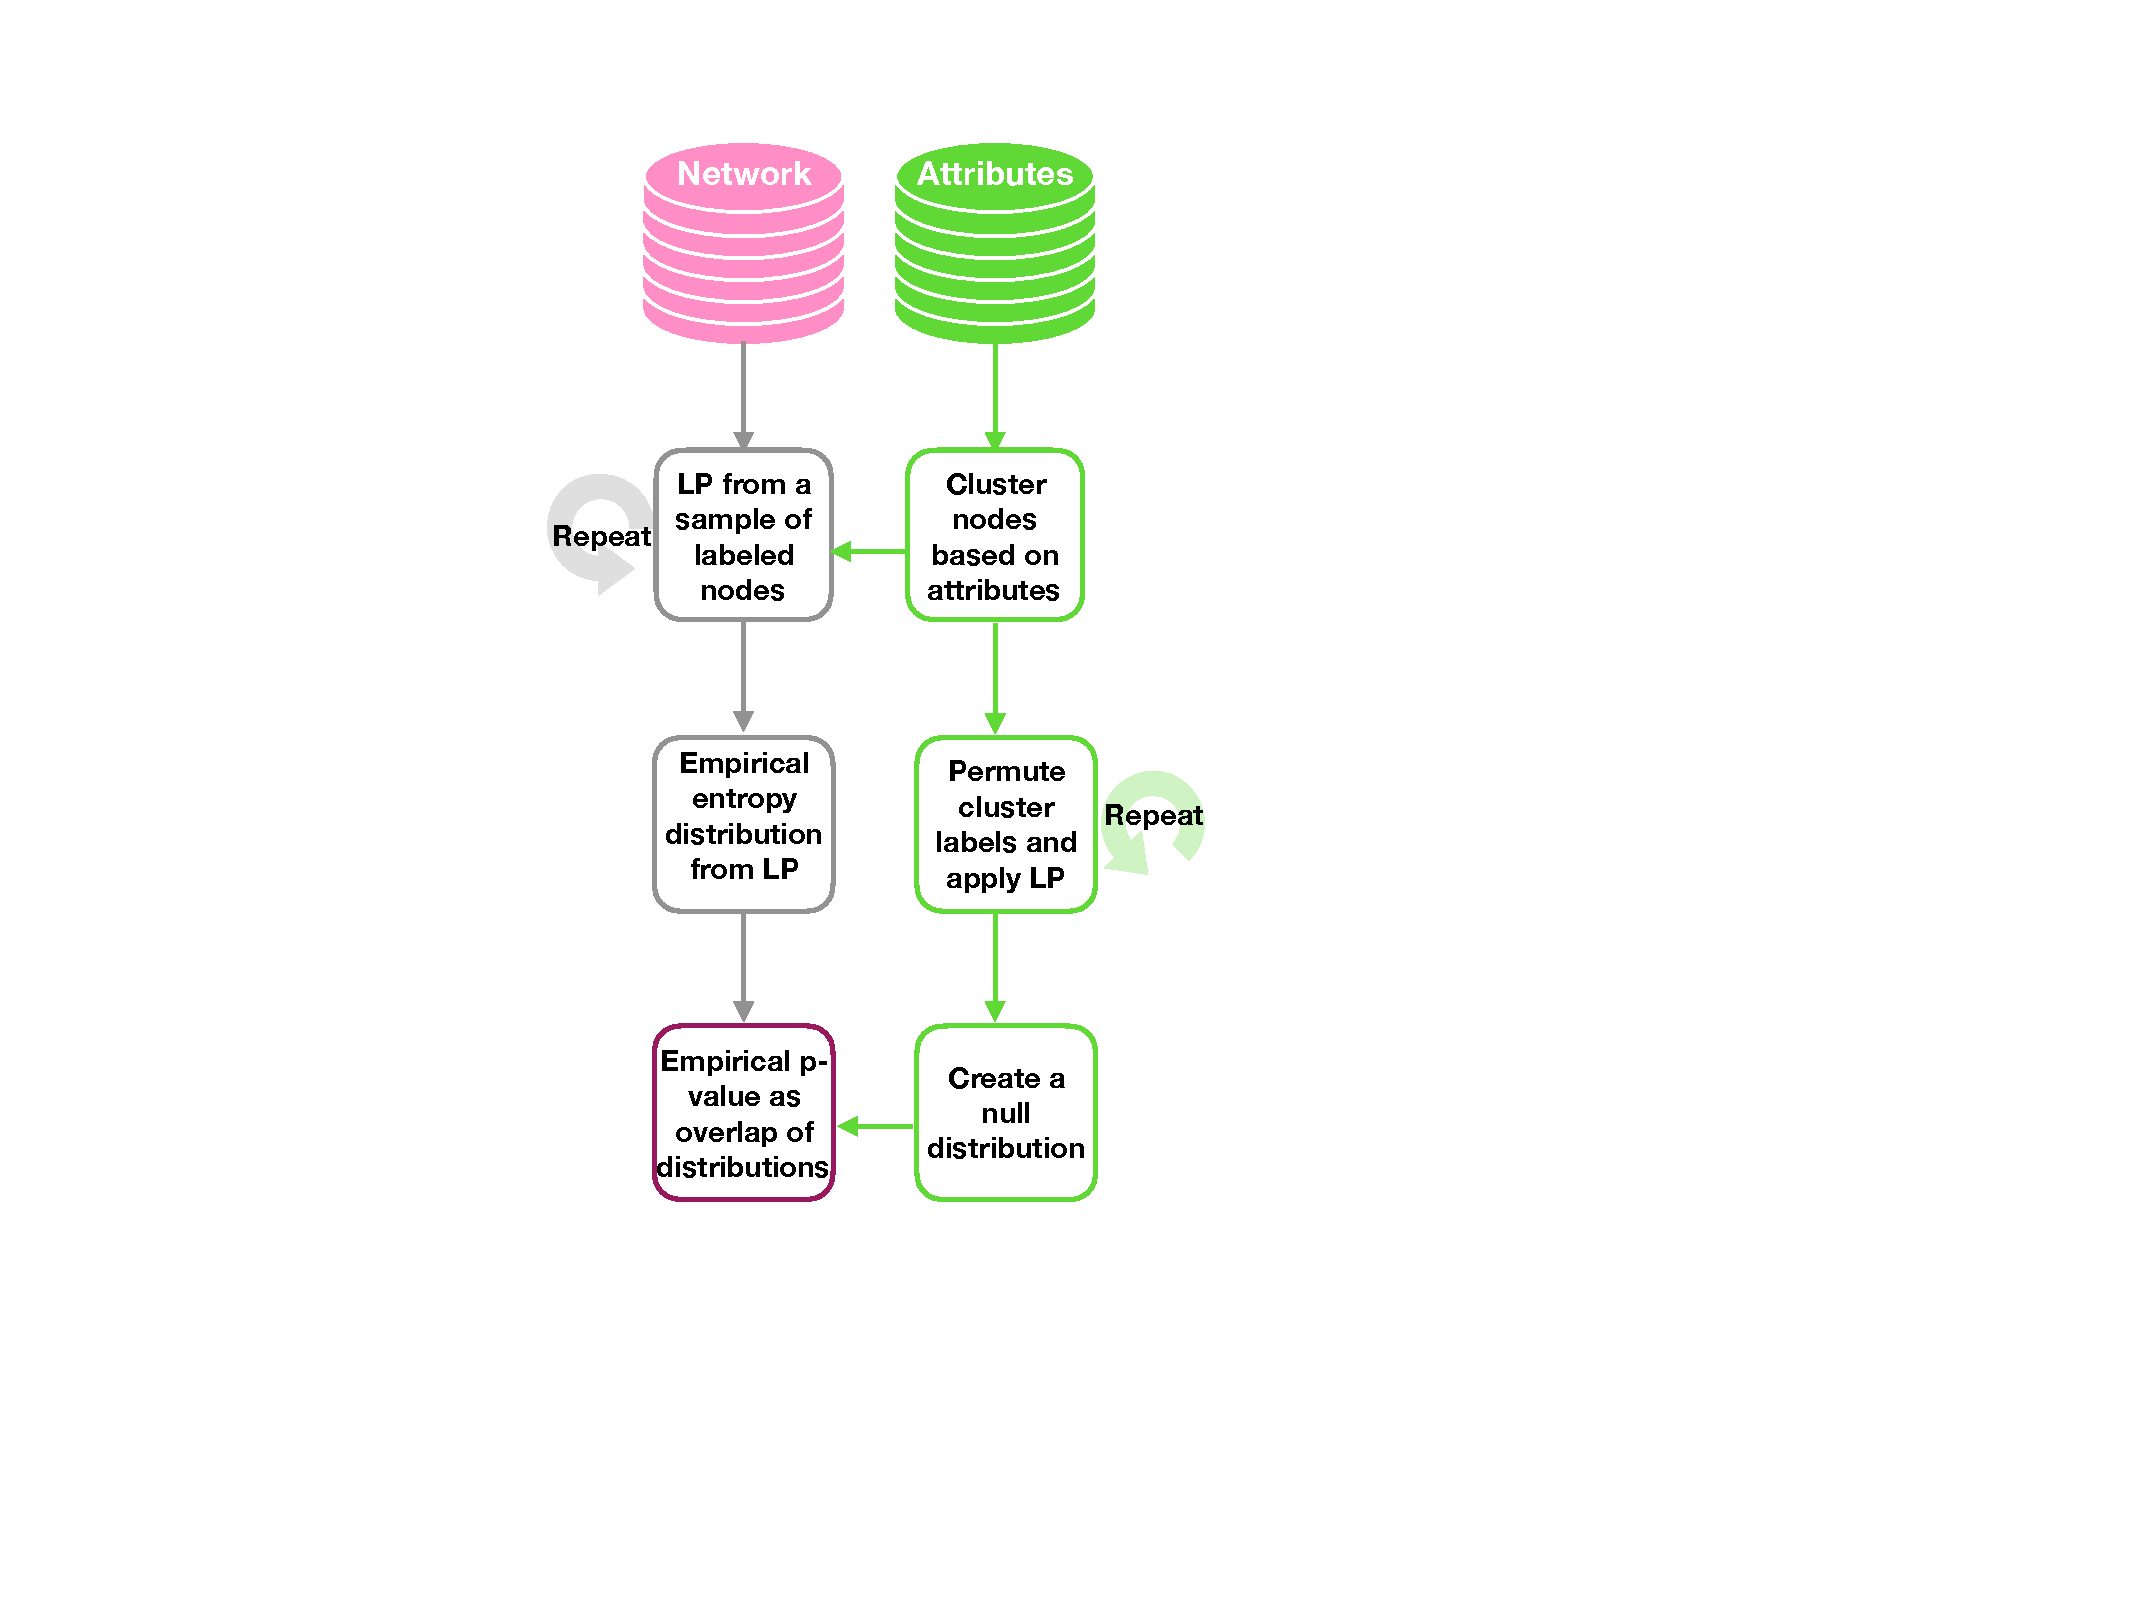
\includegraphics[scale=0.5]{Schem.pdf}
\caption{{\bf Overview of the method}. Our test first labels the nodes according to attribute information, $\tilde{{\bf z}}$. Then in a collection of $T$ trials, a sample of $l$ nodes is treated as labeled, according to $\tilde{{\bf z}}$. In each trial, a label propagation task is performed to predict the probability distribution over communities for the unlabeled $N-l$ nodes. The entropy of the node-to-community assignment probabilities is used as an estimate of how well the attributes align with connectivity. Also in each trial, $\tilde{{\bf z}}$ is permuted and subjected to the label propagation task to compute a `null' entropy value. After repeating this process in $T$ trials, the empirical $p$-value is calculated based on the overlap between the null entropy distribution and the empirical entropy distribution.}
\label{Overview}
\end{center}
\end{figure}

\subsection{Notation}
For convenience, we define some notation that assists in setting up this problem. For a network with $N$ nodes, we let ${\bf z}$ be the $N$-length vector of node-to-community assignments, based on only the network connectivity information given in adjacency matrix, ${\bf A}$. This implies that the $i$-th entry, $z_{i}$ gives the community assignment for node $i$. Alternatively, when nodes are labeled according to the attribute information, we denote their community assignments with $\tilde{{\bf z}}$.  Finally, our permutation test involves taking a subset of nodes and their labels in $\tilde{{\bf z}}$ to treat as the \emph{labeled} nodes and propagate the labels out to the unlabeled nodes. We denote this distinction by $\tilde{{\bf z}}^{L}$ and $\tilde{{\bf z}}^{U}$, denoting the community labels for the labeled and unlabeled subsets, respectively. Finally, we assume that each node has $p$ associated attributes, which are stored in the $N \times p$ matrix, ${\bf X}$. That is, the $i$th row of ${\bf X}$, $X_{i}$ gives the values of the $p$ attributes for node $i$. 

\subsection{Classifying Nodes}
The first step is to classify nodes according to attributes, denoted by $\tilde{{\bf z}}$. We assume some prior knowledge for the $K$, specifying many communities are in the data, hence each $\tilde{{\ z}}_{i}$ takes on 1 of $K$ values. In the case where nodes are classified discretely, according to a single source of information, this labeling occurs without any effort. In the case where each node has multiple attributes, we have found that a simple clustering method, such as $k$-means works well. 

\subsection{Sampling Nodes and Creating Entropy Distributions}
In the sampling step, for a large number of trials, $S$, we randomly select $l$ nodes, $\{L\}$ and their corresponding labels, $\tilde{{\bf z}}^{L}$. From here, we seek to predict the labels for the the remaining $N-l$ nodes that comprise the unlabeled set, $\{U\}$, with labels $\tilde{{\bf z}}^{L}$. 

\indent After splitting all $N$ nodes into their labeled an unlabeled sets, we use the label propagation approach described by Zhu \emph{et al.,} \cite{learning } to generate a probability distribution for each of the nodes in $\{U\}$. Ultimately, we seek to define the $N \times K$ matrix, ${\bf Y}$, where $Y_{ic}$ is the probability that node $i$ belongs to class $c$. We can split this matrix into two matrices, ${\bf Y}^{L}$ and ${\bf Y}^{U}$ with the containing the subset of rows corresponding to nodes in $\{L\}$ and $\{U\}$, respectively. Therefore, the label propagation task is to effectively estimate ${\bf Y}^{U}$. We use $\tilde{{\bf z}}^{L}$ to initialize ${\bf Y}^{L}$ so that for node $i$, with $\tilde{{z}_{i}}^{L}=c$, $Y^{L}_{ic}=1$ and all other elements in the row are 0.   

 To compute ${\bf Y}^{U}$, we first compute the row-normalized adjacency matrix, ${\bar{\bf A}}$. That is, $\bar{A_{ij}}=A_{ij}/\sum_{t}A_{it}$. We then rearrange $\bar{A_{ij}}$ so that the first $l$ rows and columns correspond to the labeled nodes, and the next $N-l$ rows and columns correspond to the unlabeled nodes. To do this, ${\bf A}$ is split into 4 submatrices after the $l$th row and $l$th column.That is, we write ${\bar{\bf A}}$ as,
 
%\begin{equation}
${\bar{\bf A}}=
\begin{bmatrix}
 \bar{A}_{ll} & \bar{A}_{lu} \\
 \bar{A}_{ul} & \bar{A}_{uu} \\
 \end{bmatrix}$.
 
 From here, we iteratively update ${\bf Y}^{U}$ according to the update rule provided by Zhu \emph{et al.,} \cite{learning} as,
 
 \begin{equation}
 \label{FP}
 {\bf Y}^{U} \leftarrow {\bar A}_{uu}{\bf Y}^{U}+{\bar A}_{ul}{\bf Y}_{L}.
 \end{equation}
 
 In practice, ${\bf Y}^{U}$ is continuously updated until convergence. 
 
 Computing ${\bf Y}^{U}$ for one pair of ${\bf L}$ and ${\bf U}$ comprises the true label propagation task of one trial. To generate our null distribution, we first permute the entries of $\tilde{{\bf z}}^{L}$, and denote this permuted version as $\tilde{{\bf z}}_{\text{perm}}^{L}$. Just as we showed in the true label propagation task, we use $\tilde{{\bf z}}_{\text{perm}}^{L}$ to define a corresponding permuted version of ${\bf Y}_{\text{perm}}^{L}$ with $Y_{\text{perm}_{ic}}^{L}$ set to be 1 if node $i$ belongs to community $c$, under the permuted labels, given by $\tilde{{\bf z}}_{\text{perm}}^{L}$. The analogous update relationship shown in equation \ref{FP} gives ${\bf Y}_{\text{perm}}^{L}$. 
 
After computing ${\bf Y}^{U}$ and ${\bf Y}_{\text{perm}}^{U}$, the next step is to compute their corresponding entropies, $E$ and $E_{\text{perm}}$. We compute entropy $H(x)$ as,

\begin{equation}
H(x)=-\sum_{ic}p_{ic}\log(p_{ic}).
\end{equation}

Moreover, $H({\bf Y}^{U})$ and $H({\bf Y}_{\text{perm}}^{U})$ give $E$ and $E_{\text{perm}}$, respectively. We let $\mathcal{E}=\{E_{1}, E_{2}, \dots E_{T}\}$ and $\mathcal{E}_{\text{perm}}=\{E_{1}, E_{2}, \dots E_{T}\}$ be the collection of entropies over the $T$ trials. 

\subsection{Computing the empirical $p$-value}
After having performed $T$ trials, we compute the empirical $p$-value for the test and is interpreted as the overlap between $\mathcal{E}$ and $\mathcal{E}_{\text{perm}}$. In the case where attributes, ${\bf X}$ and connectivity ${\bf A}$ are well-aligned with connectivity, $\mathcal{E}$ and $\mathcal{E}_{\text{perm}}$ should not overlap because the entropy for the label propagation task should be very low. Alternatively, as ${\bf X}$ and ${\bf A}$ become less aligned, the entropy of the prediction from the label propagation task should be higher and hence $\mathcal{E}$ and $\mathcal{E}_{\text{perm}}$ will overlap. Then the empirical $p$-value, $p$ is calculated as,

\begin{equation}
p=P(\mathcal{E}_{\text{perm}}<\max(\mathcal{E})).
\end{equation}

That is, our interpretation of the empirical $p$-value is the proportion of $\mathcal{E}_{\text{perm}}$ that are less than the maximum value of $\mathcal{E}$. 

\section{Results}
We present results on synthetic networks and on a network representation of a single cell mass cytometry dataset. In this section, we seek to confirm that the empirical $p$-value leads to an accurate and interpretable conclusion. The results on synthetic data re useful because we have an understanding of when the $p$-value should be significant, due to our knowledge of how the data were generated. Similarly, in the single cell mass cytometry dataset, we use particular marker features to validate our computed empirical $p$-values. 

\subsection{Synthetic Examples}
First, we sought to verify that our empirical $p$-value was capturing desirable behavior. First, we expected the $p$-value to decrease in significance as the label propagation distribution increases in overlap with the empirical null distribution. Second, we sought to have a $p$-value that decreased in significance as the entropy of the partition increased. In Figure \ref{Align:Syn1}, we considered a network generated from a stochastic block model with $N=200$ nodes, $K=4$ communities, within-community edge probability ($p_{in}$), $p_{in}=0.6$, and between-community edge probability, ($p_{out}$), $p_{out}=0.02$. That is for a pair of nodes, $i$ and $j$, the probability of an edge existing between them is modeled as $P(A_{ij}=1)=p_{in}$ if $z_{i}=z_{j}$ and $P(A_{ij}=1)=p_{out}$ if $z_{i}\ne z_{j}$.

Associated with each node is a 3-dimensional Gaussian attribute vector, drawn from 1 of $K$ multivariate Gaussian distributions. Under this formulation, each community has its own associated multivariate Gaussian distribution and attribute vectors and a node in community $k$ is parameterized by mean ${\boldsymbol \mu}_{k}=[\mu_{1},\mu_{2},\mu_{3}]$ and covariance matrix ${\boldsymbol \Sigma}_{k}$.
 
 To generate each ${\boldsymbol \mu}_{k}=[\mu_{1},\mu_{2},\mu_{3}]$, we draw each $\mu_{d}$ from a standard Normal distribution with mean 0 and unit variance. For a community $k$, ${\boldsymbol \Sigma}_{k}$ is also the identify covariance matrix.

\begin{figure*}
\centering
\begin{center}
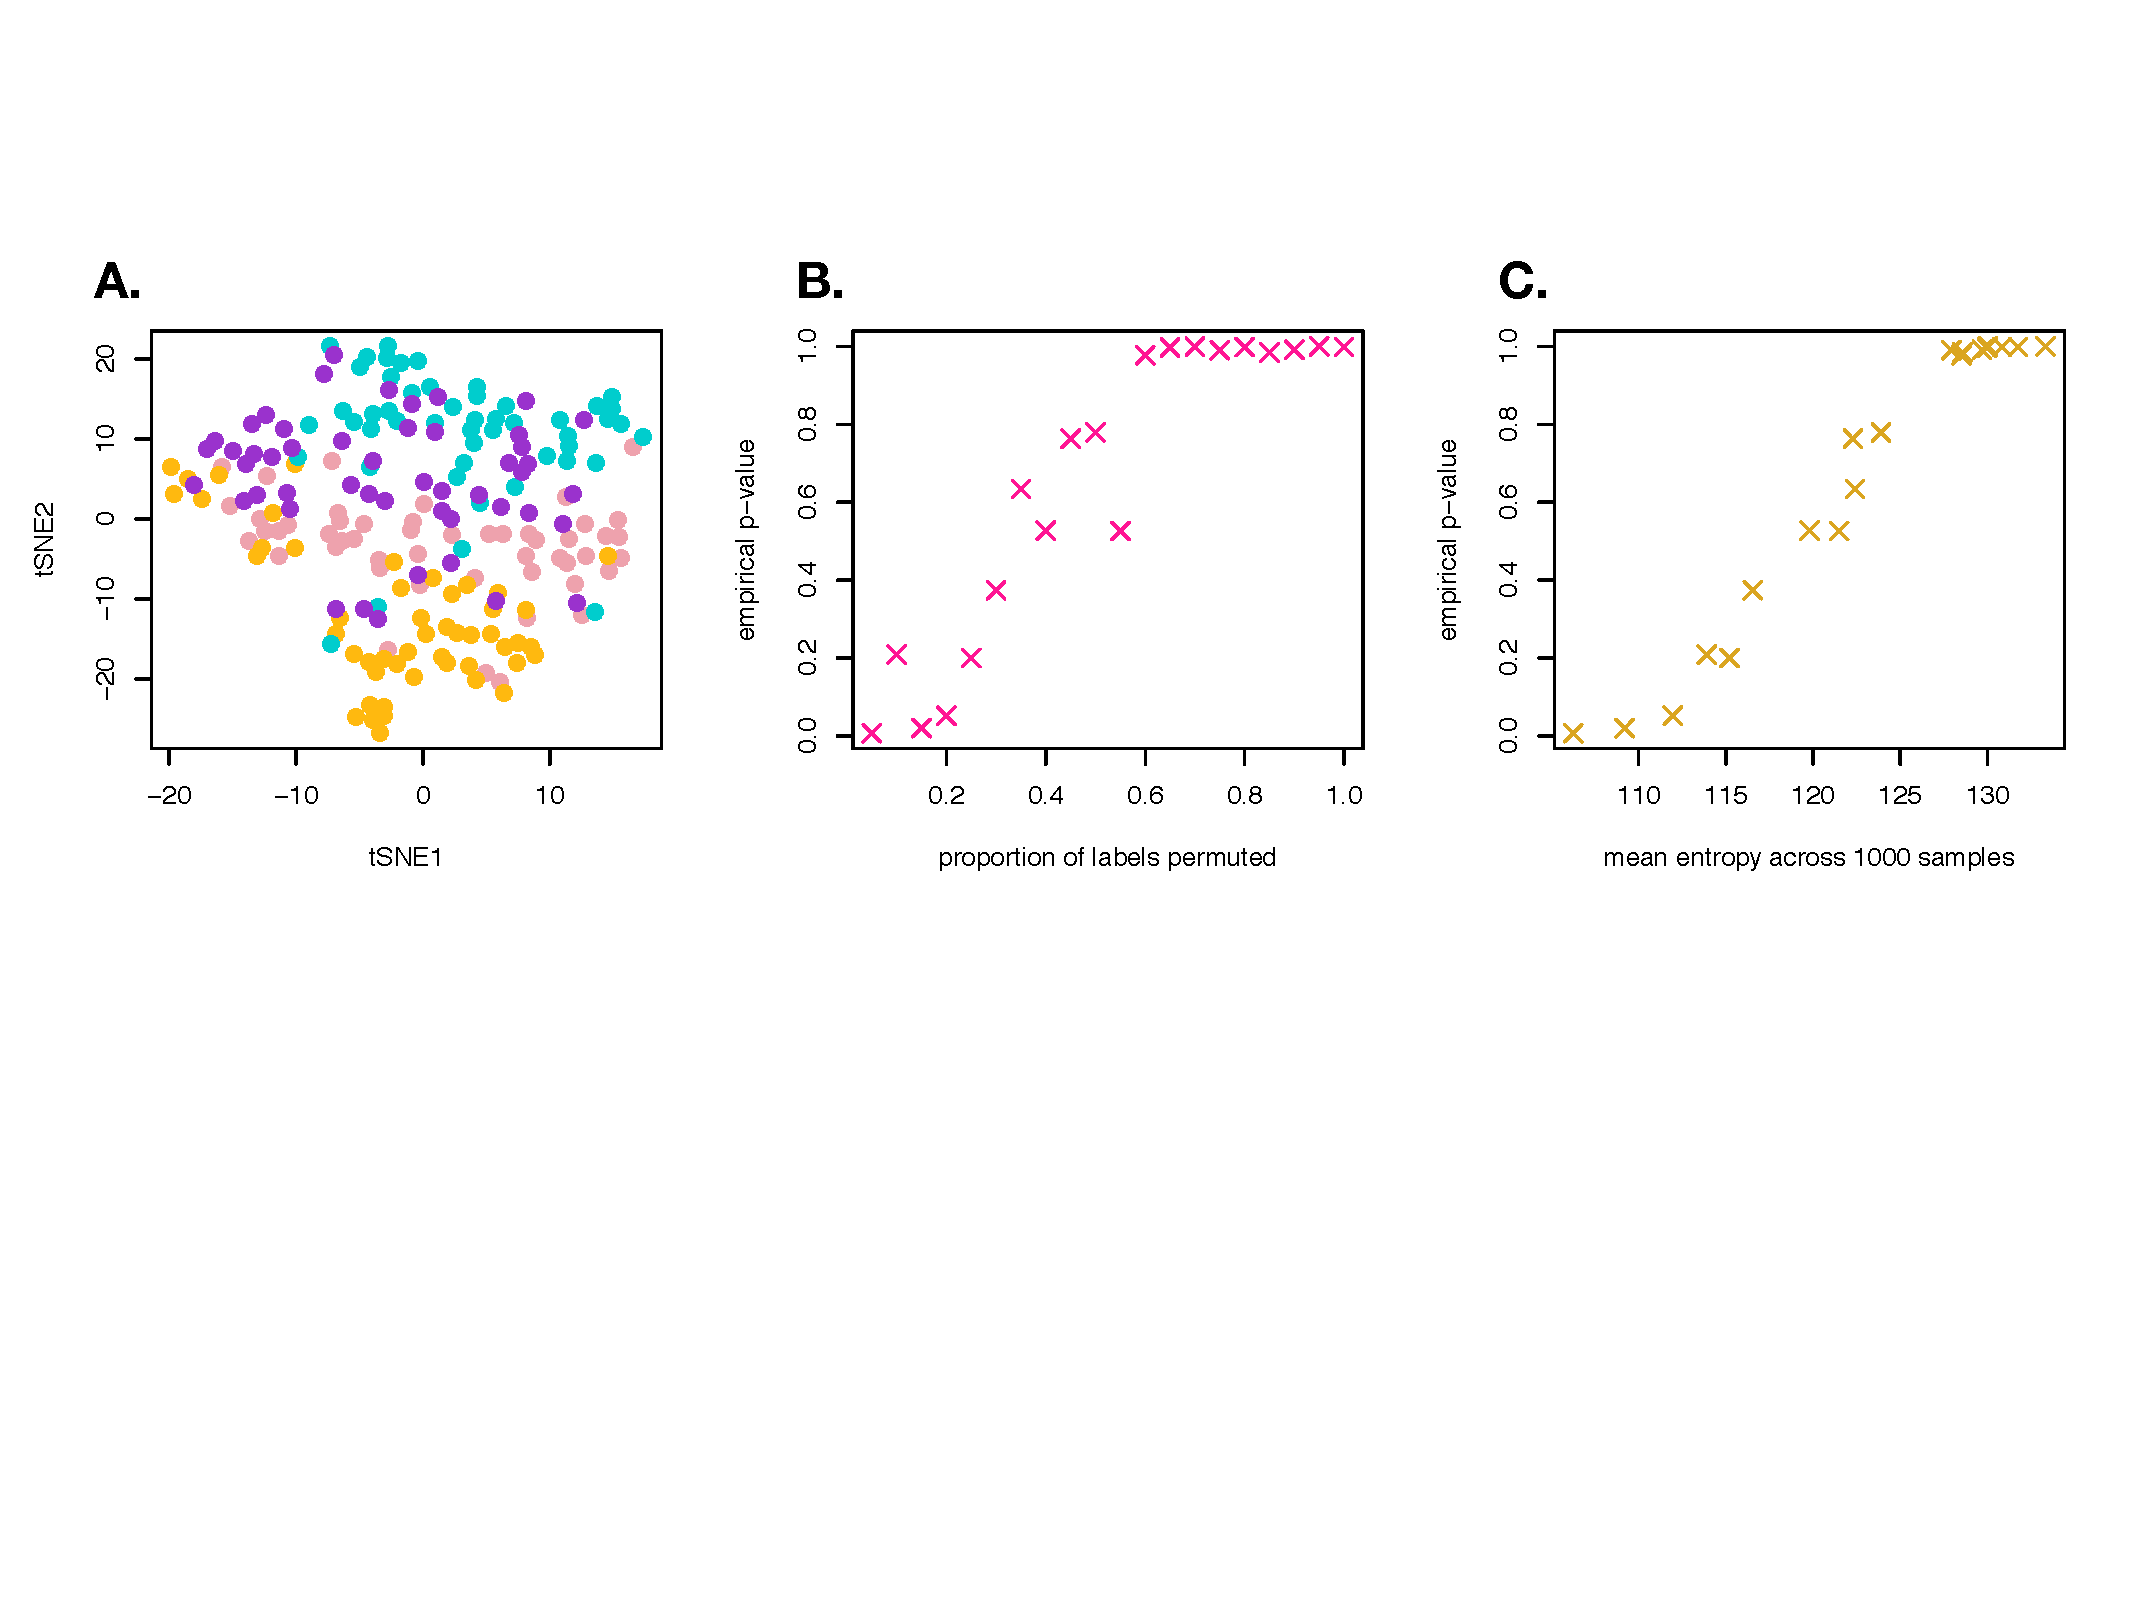
\includegraphics[width=.9\textwidth]{SimpleSynthetic.pdf}
\caption{{\bf Properties of the empirical $p$-value.} To understand the properties of our empirical $p$-value, we generated a synthetic network, ${\bf A}$ from an SBM with $N=200$ nodes, $K=4$. The vector of continuous attributes for a node $i$, ($X_{i}$) was drawn from a multivariate Gaussian distribution parameterized by its community assignment (${\bf z}$) or $\{{\boldsymbol \mu}_{z_{i}}, {\boldsymbol \Sigma}_{z_{i}}\}$. In these experiments, we permuted varying fractions of $\tilde{{\bf z}}$ and observed the effects on entropy and empirical $p$-value. {\bf A}. We used tSNE to visualize the two dimensional projection of the 200 nodes. For the most part, members of the same community cluster together. {\bf B.} We plotted the empirical $p$-value as a function of the proportion of labels permuted and observed decreased statistical significance (increased empirical $p$-value) with an increasing proportion of permuted labels. {\bf C.} We plotted the empirical $p$-value as a function of the mean entropy ($\mathcal{E}$) across $T=1000$ trials used to generate the entropy distributions for each experiment. Increased entropy corresponding to a larger proportion of $\tilde{\bf z}$ permuted leads to a decreased $p$-value.}
\label{Align:Syn1}
\end{center}
\end{figure*}

When performing our label propagation task, we used a sample of $S=1000$ nodes and repeated the experiment $T=1000$ times. \\
\indent First, we visualized the distribution of the attributes, using a 2-dimensional projection with tSNE \cite{TwoD}. In Figure \ref{Align:Syn1}A., each point represents a node and is colored by its community assignment, ${\bf z}$. We can see that there are clearly clusters of nodes from the same community, but there is also a some mixing. To test how the empirical $p$-value behaved as the label propagation distribution converged to the null distribution, we experimentally perturbed various proportions of the node labels based on attributes ($\tilde{\bf z}$) that were input to the label propagation task. This test was implemented to verify that with a higher proportion of permuted entries in $\tilde{\bf z}$, the empirical entropy distributions, $\mathcal{E}$ and $\mathcal{E}_{\text{perm}}$ would have more extensive overlap. As expected, in Figure \ref{Align:Syn1}B., we observed that by permuting a larger proportion of the labels, $\tilde{\bf z}$, there was an associated increase in the empirical $p$-value (decreased significance). Finally, in Figure \ref{Align:Syn1}C. we examined the relationship between the average entropy across each element of $\mathcal{E}$ obtained over the 1000 simulations, and the empirical $p$-value. As expected, these quantities are highly related, with a higher entropy leading to a more significant empirical $p$-value.


\subsubsection{Comparison to BESTest}
We used the synthetic data from the experiment described in Figure \ref{Align:Syn1} to compare our results to those obtained using BESTest. BESTest is the method developed by Peel \emph{et al.}, to inform their attributed neoSBM model of how informative attributes are on community structure \cite{peel2017ground}. BESTest works first by labeling the nodes according to $\tilde{\bf z}$, based on the attribute information. Under this partition of the nodes, the SBM parameters are optimized, where the maximum likelihood estimate for the connection probability between a pair of communities $r$ and $s$ is given by $\hat{\omega}_{rs}$. This maximum likelihood estimate $\hat{\omega}_{rs}$ is computed as $\hat{\omega}_{rs}=m_{rs}/n_{r}n_{s}$. Here, $m_{rs}$ is the number of edges between communities $r$ and $s$, while $n_{r}$ and $n_{s}$ are the number of nodes in communities $r$ and $s$, respectively. The entropy, $\mathcal{H}$ of this partition across the communities is computed as,

\begin{equation}
\mathcal{H}({\tilde{\bf z}})=-\frac{1}{2}[\sum_{rs}\log \hat{\omega}_{rs}+(n_{r}n_{s}-m_{rs})\log(1-\hat{\omega}_{rs})]+O(N^{-1}). 
\end{equation}

The empirical $p$-value is computed with BESTest through a permutation test which computes $\mathcal{H}({\tilde{\bf z}}_{\text{perm}})$ many times and reports the fraction of $\mathcal{H}({\tilde{\bf z}}_{\text{perm}})<\mathcal{H}({\tilde{\bf z}})$. This method is appropriate and useful for the attributed SBM. We distinguish our method because it is testing alignment of the connectivity in genera and does not make an assumption about the stochastic block model being an appropriate model for the data. 

Varying proportions of the attribute labels allowed us to examine different levels of entropy on the partition of a held-out set. We used $T=1000$ permutations to compute the BESest empirical $p$-value. In Figure \ref{BestCompare}A., we looked at the relationship between the $p$-value under the LP test (horizontal axis) and from BESTest (vertical axis). We see that there is broader range of $p$-values with LP, in comparison to BESTest, which seems to jump quickly from not-significant to significant. In Figure \ref{BestCompare}B., we plotted the BestTest empirical $p$-value as a function of the BESTest entropy. We observed a pattern very similar to Figure \ref{BestCompare}A., where a wide range of entropies across experiments are not reflected in a continuously changing $p$-value. Next, we sought to understand how the BESTest entropy compared with the $p$-values computed with LP. In Figure \ref{BestCompare}C., we observe a wider range of $p$-values across the continuum of observed entropies. Finally, in Figure \ref{BestCompare}D. , we examined the relationship between LP and BESTest entropies and found them to well correlated ($r=0.95$). This suggests that both tests are capturing the same level of uncertainty, but the interpretation of the empirical $p$-value differs. 

\begin{figure*}
\centering
\begin{center}
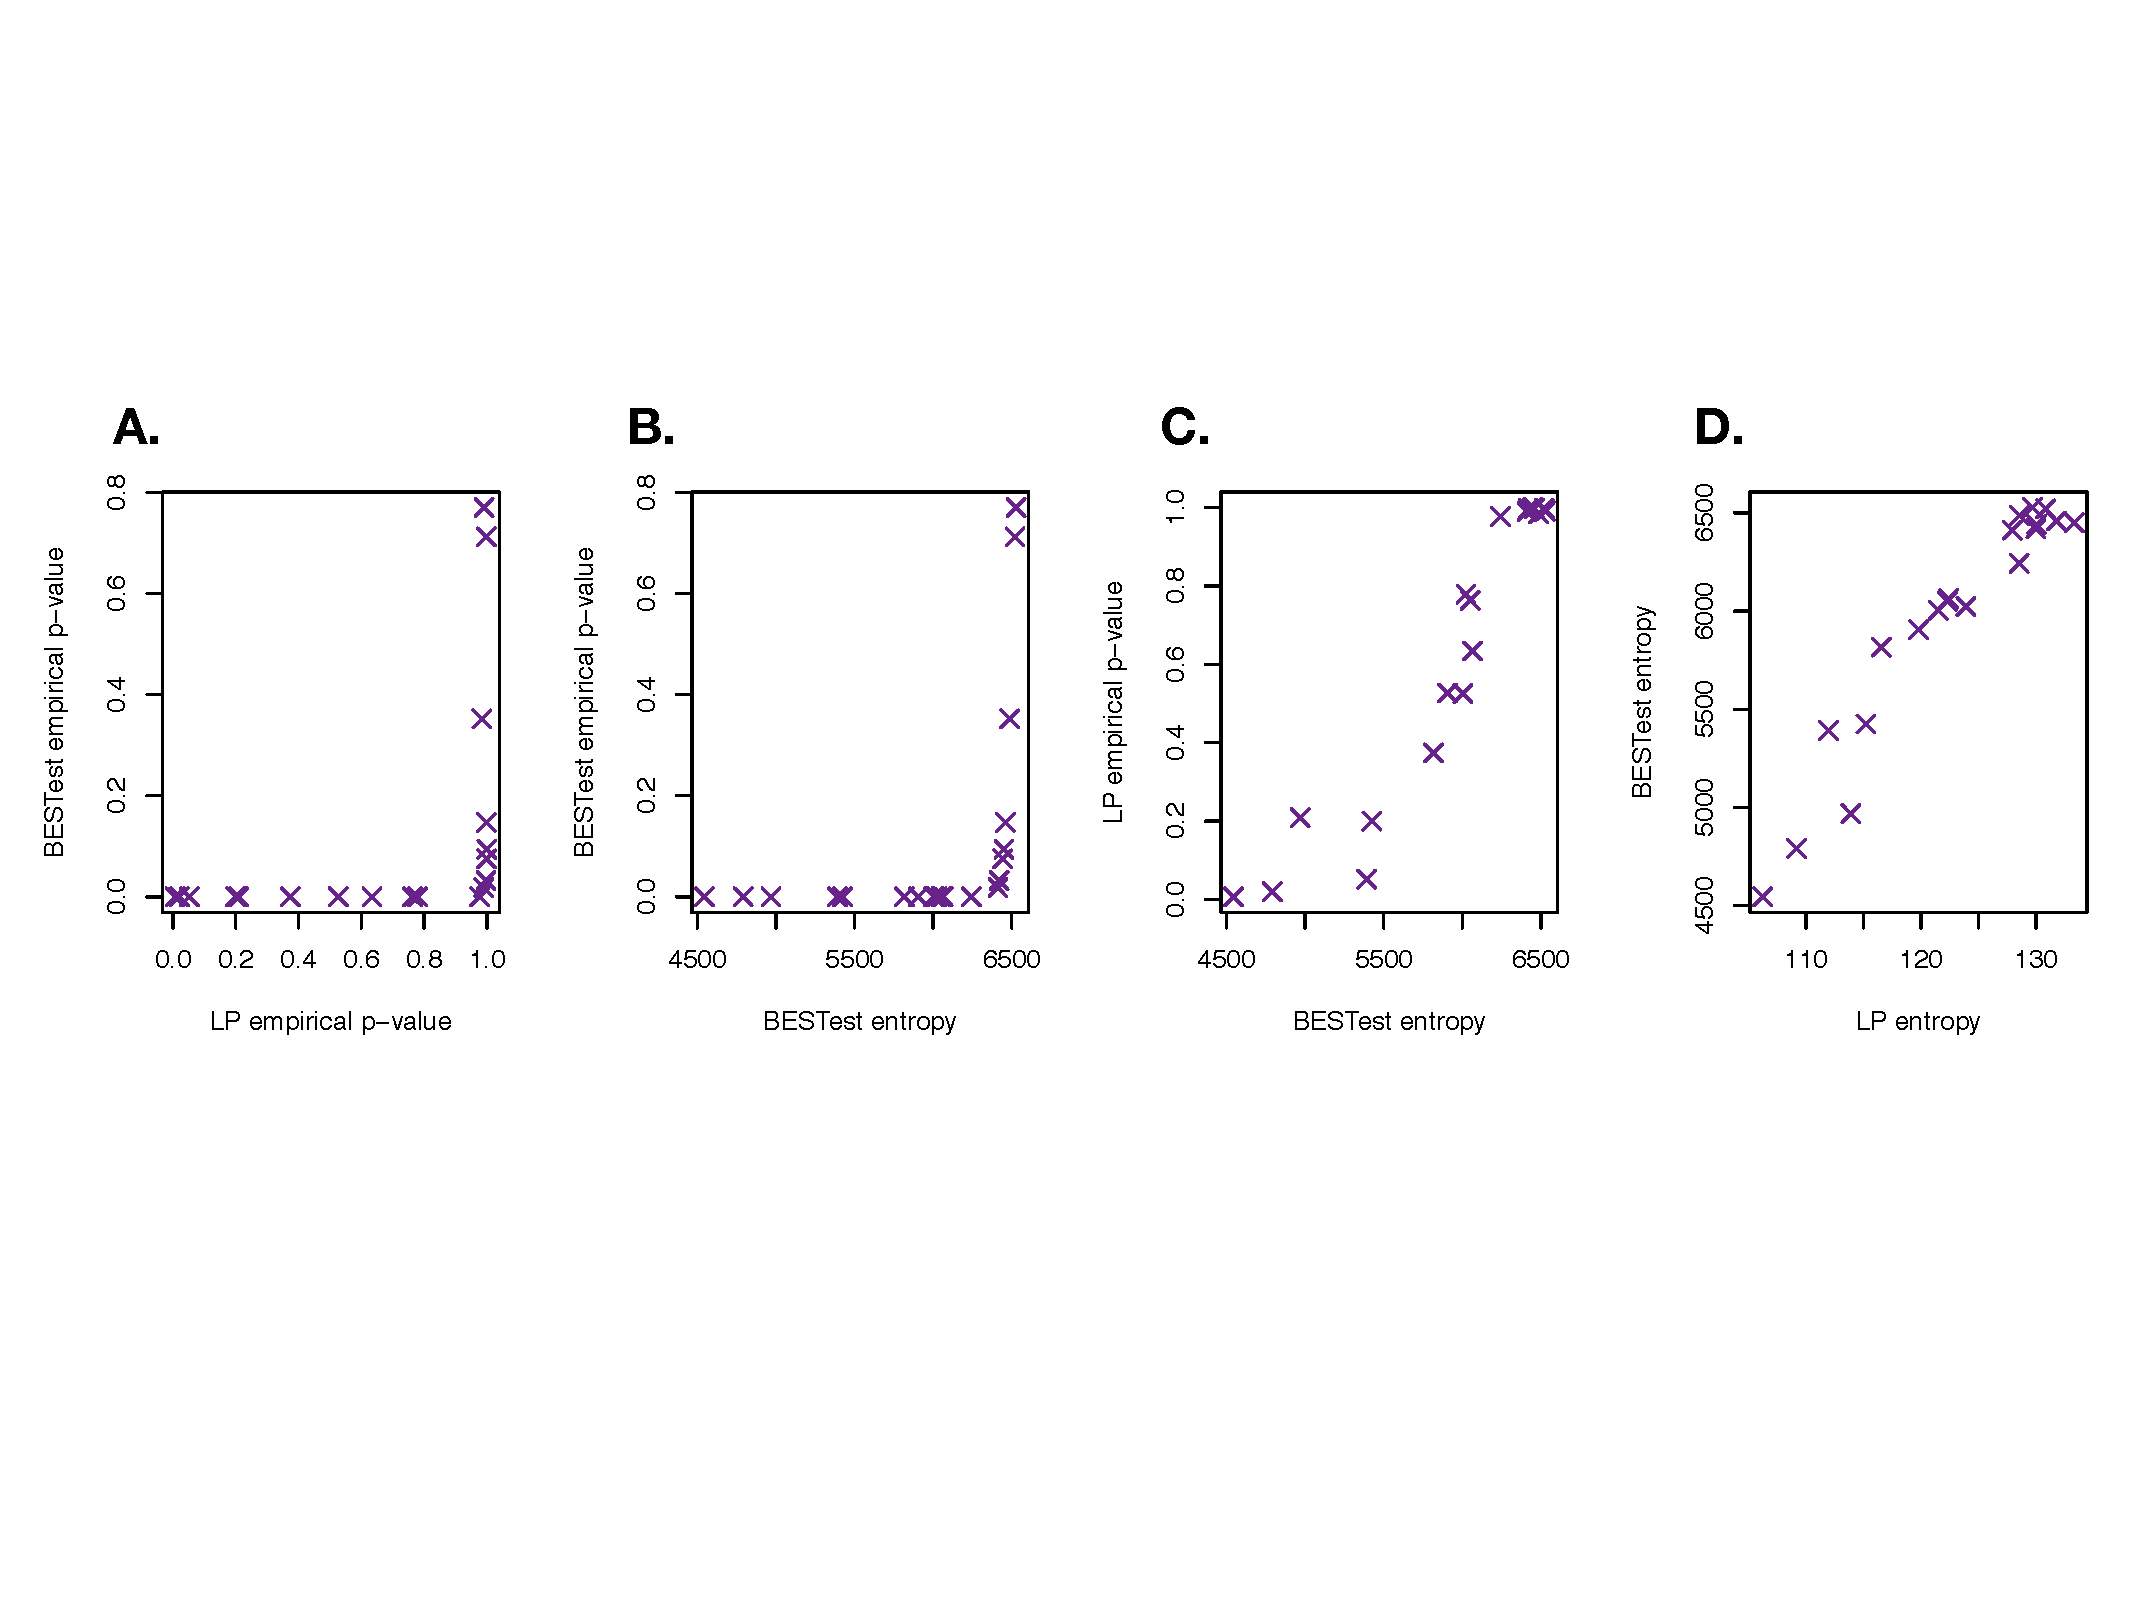
\includegraphics[width=.9\textwidth]{BestCompare.pdf}
\caption{{\bf Comparison with BESTest.} We sought to understand the relationship between our empirical $p$-value and that computed according to BESTest. To study this, we used the same experiment described in Figure \ref{Align:Syn1}, where we varied the proportion of permuted labels from $\tilde{\bf z}$. We denote our empirical $p$-value by `LP empirical $p$-value. {\bf A.} We plotted the BESTest empirical $p$-value against our LP empirical $p$-value. {\bf B.} We plotted the BESTest empirical $p$-value as a function of the BESTest entropy. BESTest gives a significant empirical $p$-value for a much wider range of entropy levels than our test. {\bf C.} The experiments produced a wide range of entropies under BESTest, which are captured by corresponding differences in our empirical $p$-value. {\bf D.} We compared the BESTest approach to computing entropy to our LP method and observed a high correlation between these entropy measures $(r=0.95)$. }
\label{BestCompare}
\end{center}
\end{figure*}


\subsubsection{Strength of community structure} Now we explored how structural communities, according to connectivity, influence the entropy and corresponding empirical $p$-values. We refer to a strong community structure as one that has many within-community connections and few between-community connections. To approximate this, we considered the $p_{in}$ to $p_{out}$ ratio for a stochastic block model. As previously described, $p_{in}$ is defined as the probability of observing an edge between a pair of nodes in the same community, while $p_{out}$ is the probability of observing an edge between a pair of nodes in different communities. We expected that the entropy and empirical $p$-value would increase with an increasing $p_{in}/p_{out}$ ratio. That is, as the community structure becomes less prominent with an increased number of connections between communities, the label propagation task should become more difficult. To study this with synthetic data, we varied the $p_{in}/p_{out}$ ratio, by considering a four community stochastic block model with values of $p_{in}$ between 0.05 and 0.45 and choosing a corresponding $p_{out}$, such that the mean degree was equal 30.  For each pair of $p_{in}$ and $p_{out}$, we generated 10 synthetic stochastic block models. Accompanying each synthetic network was a fixed 3-dimensional attribute matrix, ${\bf X}$, where the attribute vectors for the members of community $k$ were drawn from a 3-dimensional multivariate Gaussian, paramertized by $\{{\boldsymbol \mu}_{k},{\boldsymbol \Sigma}_{k}\}$. For each synthetic network, we computed the entropy under our label propagation method and the corresponding $p$-value. 

\indent In Figure \ref{Pin}A., we plot the mean LP entropy over the $T=1000$ samples used to construct the empirical entropy distribution, $\mathcal{E}$, across the 10 networks for each set of $p_{in}$ and $p_{out}$. The shaded region denotes the standard deviation of the LP entropy. As the ratio between $p_{in}$ and $p_{out}$ increases, the empirical LP entropy decreases. We see a similar effect in Figure \ref{Pin}B., where we plot the empirical $p$-value as a function of the $p_{in}/p_{out}$ ratio. In this plot, the shaded region denotes the standard deviation of the empirical $p$-value. Here, a significant $p$-value (at $\alpha=0.05)$ was reached (implying attributes and connectivity are aligned) when $p_{in}/p_{out} \approx 5$. Finally in Figure \ref{Pin}C., we examined the relationship between the mean entropy and the associated mean empirical $p$-value across the 10 networks generated under each parameter pair. These values were strongly correlated ($r=0.91$).  

\begin{figure}
\centering
\begin{center}
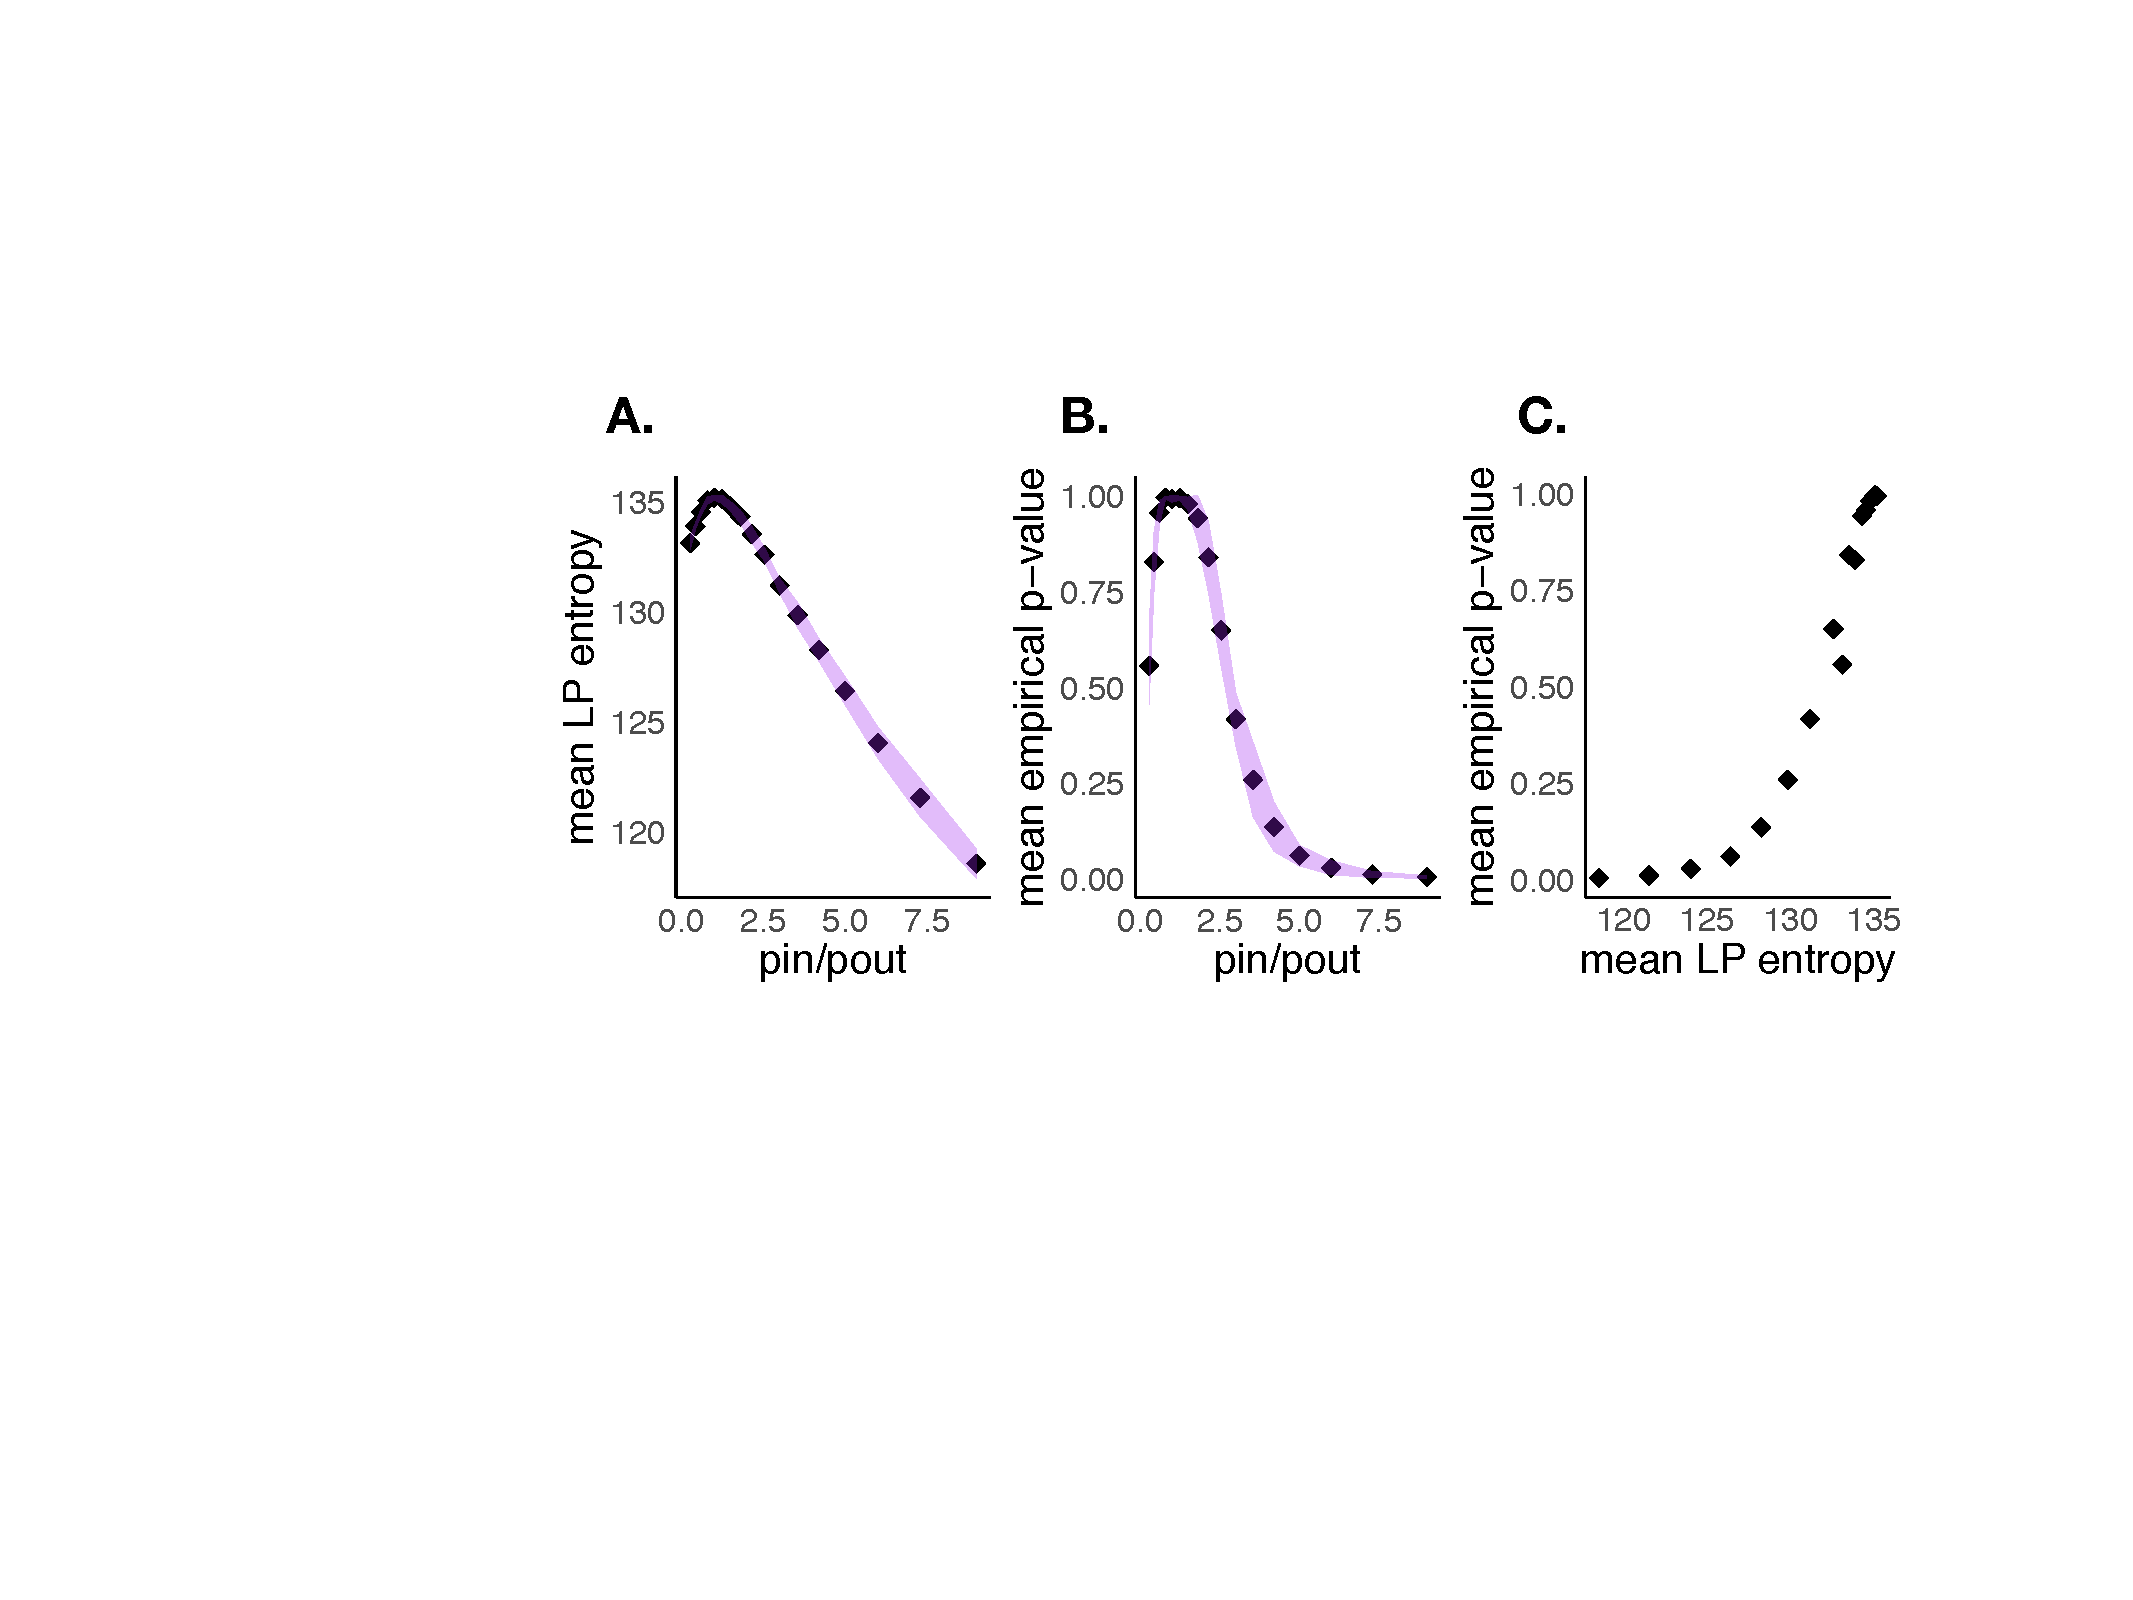
\includegraphics[width=0.9\textwidth]{PinPout.pdf}
\caption{{\bf Analysis of the strength of structural communities.} To understand the effect of network structure on our test, we generated synthetic networks from stochastic block models with various $p_{in}$ (within-community) and $p_{out}$ (between-community) parameters. Networks were generated with $p_{in}$ varying between 0.05 and 0.45 and we chose a corresponding $p_{out}$ such that the mean degree was 30. We used $p_{in}/p_{out}$ as a proxy for the strength of community, with a higher value of this ratio indicating a stronger community structure with more within-community edges and fewer between community edges. For each $p_{in}$, $p_{out}$ combination, we generated 10 synthetic network realizations. {\bf A.} We plotted the relationship between our LP entropy and $p_{in}/p_{out}$. The shaded area denotes standard deviation of the mean entropy over the 10 networks for each $p_{in}$, $p_{out}$ combination. {\bf B.} Similar to ({\bf A.}), we plotted the mean empirical $p$-value over the $T=1000$ trials used to generate the entropy distributions, $\mathcal{E}$ and $\mathcal{E}_{\text{perm}}$. For large $p_{in}/p_{out}$, the empirical $p$-value became more significant. The shaded area denotes standard deviation of empirical $p$-value over the 10 networks for each $p_{in}$, $p_{out}$ combination. {\bf C.} Finally, we plotted the relationship between the mean entropy over the $T$=1000 trials, $\mathcal{E}$ and the empirical $p$-value. These values are strongly correlated with $r=0.91$. }
\label{Pin}
\end{center}
\end{figure}

\subsection{Mass Cytometry Network Example}
We also applied our test to a mass cytometry dataset. Mass cytometry \cite{cytof} is an immunological profiling technique that gives simultaneous quantification of various immune features, such as, cell type abundances and signaling information. We used a freely available mass cytometry dataset, originally described in Ref. \cite{wong2015}, but pre-processed in an R tool called CytofKit \cite{cytofkit}. The dataset profiles 51 immune features across single cells on human T helper (T(H)) cells from peripheral blood and tonsils, which have shown to be heterogeneous within a sample. To untangle the heterogeneity and infer cellular phenotypes, dimension reduction and clustering are applied to single cell data. In this pursuit, the objective is to cluster the single cells into predicted phenotypes, based on the measured features. A powerful way to segment the single cells into their respective phenotypes is by constructing a similarity network between the cells and clustering with community detection. This method for studying single cell data is called PhenoGraph and is described in Ref. \cite{phenoGraph}. We studied the data in an analogous way by constructing a $5$-nearest neighbor network and applying community detection. To do this, each cell is connected to its 5 nearest neighbors, based on euclidean distance on the pairwise Euclidean distance for the 51 features. In this particular dataset, we considered a subset of 1000 single cells and their 51 measured features. After constructing the network, we predicted phenotypes by identifying communities (${\bf z}$) with the Louvain algorithm \cite{blondel}. Applying the Louvain algorithm identified 10 communities.  As shown in \cite{cytofkit}, one further analysis after clustering the single cells is to identify marker features with discriminative power between the inferred phenotypes. 

\begin{figure*}
\centering
\begin{center}
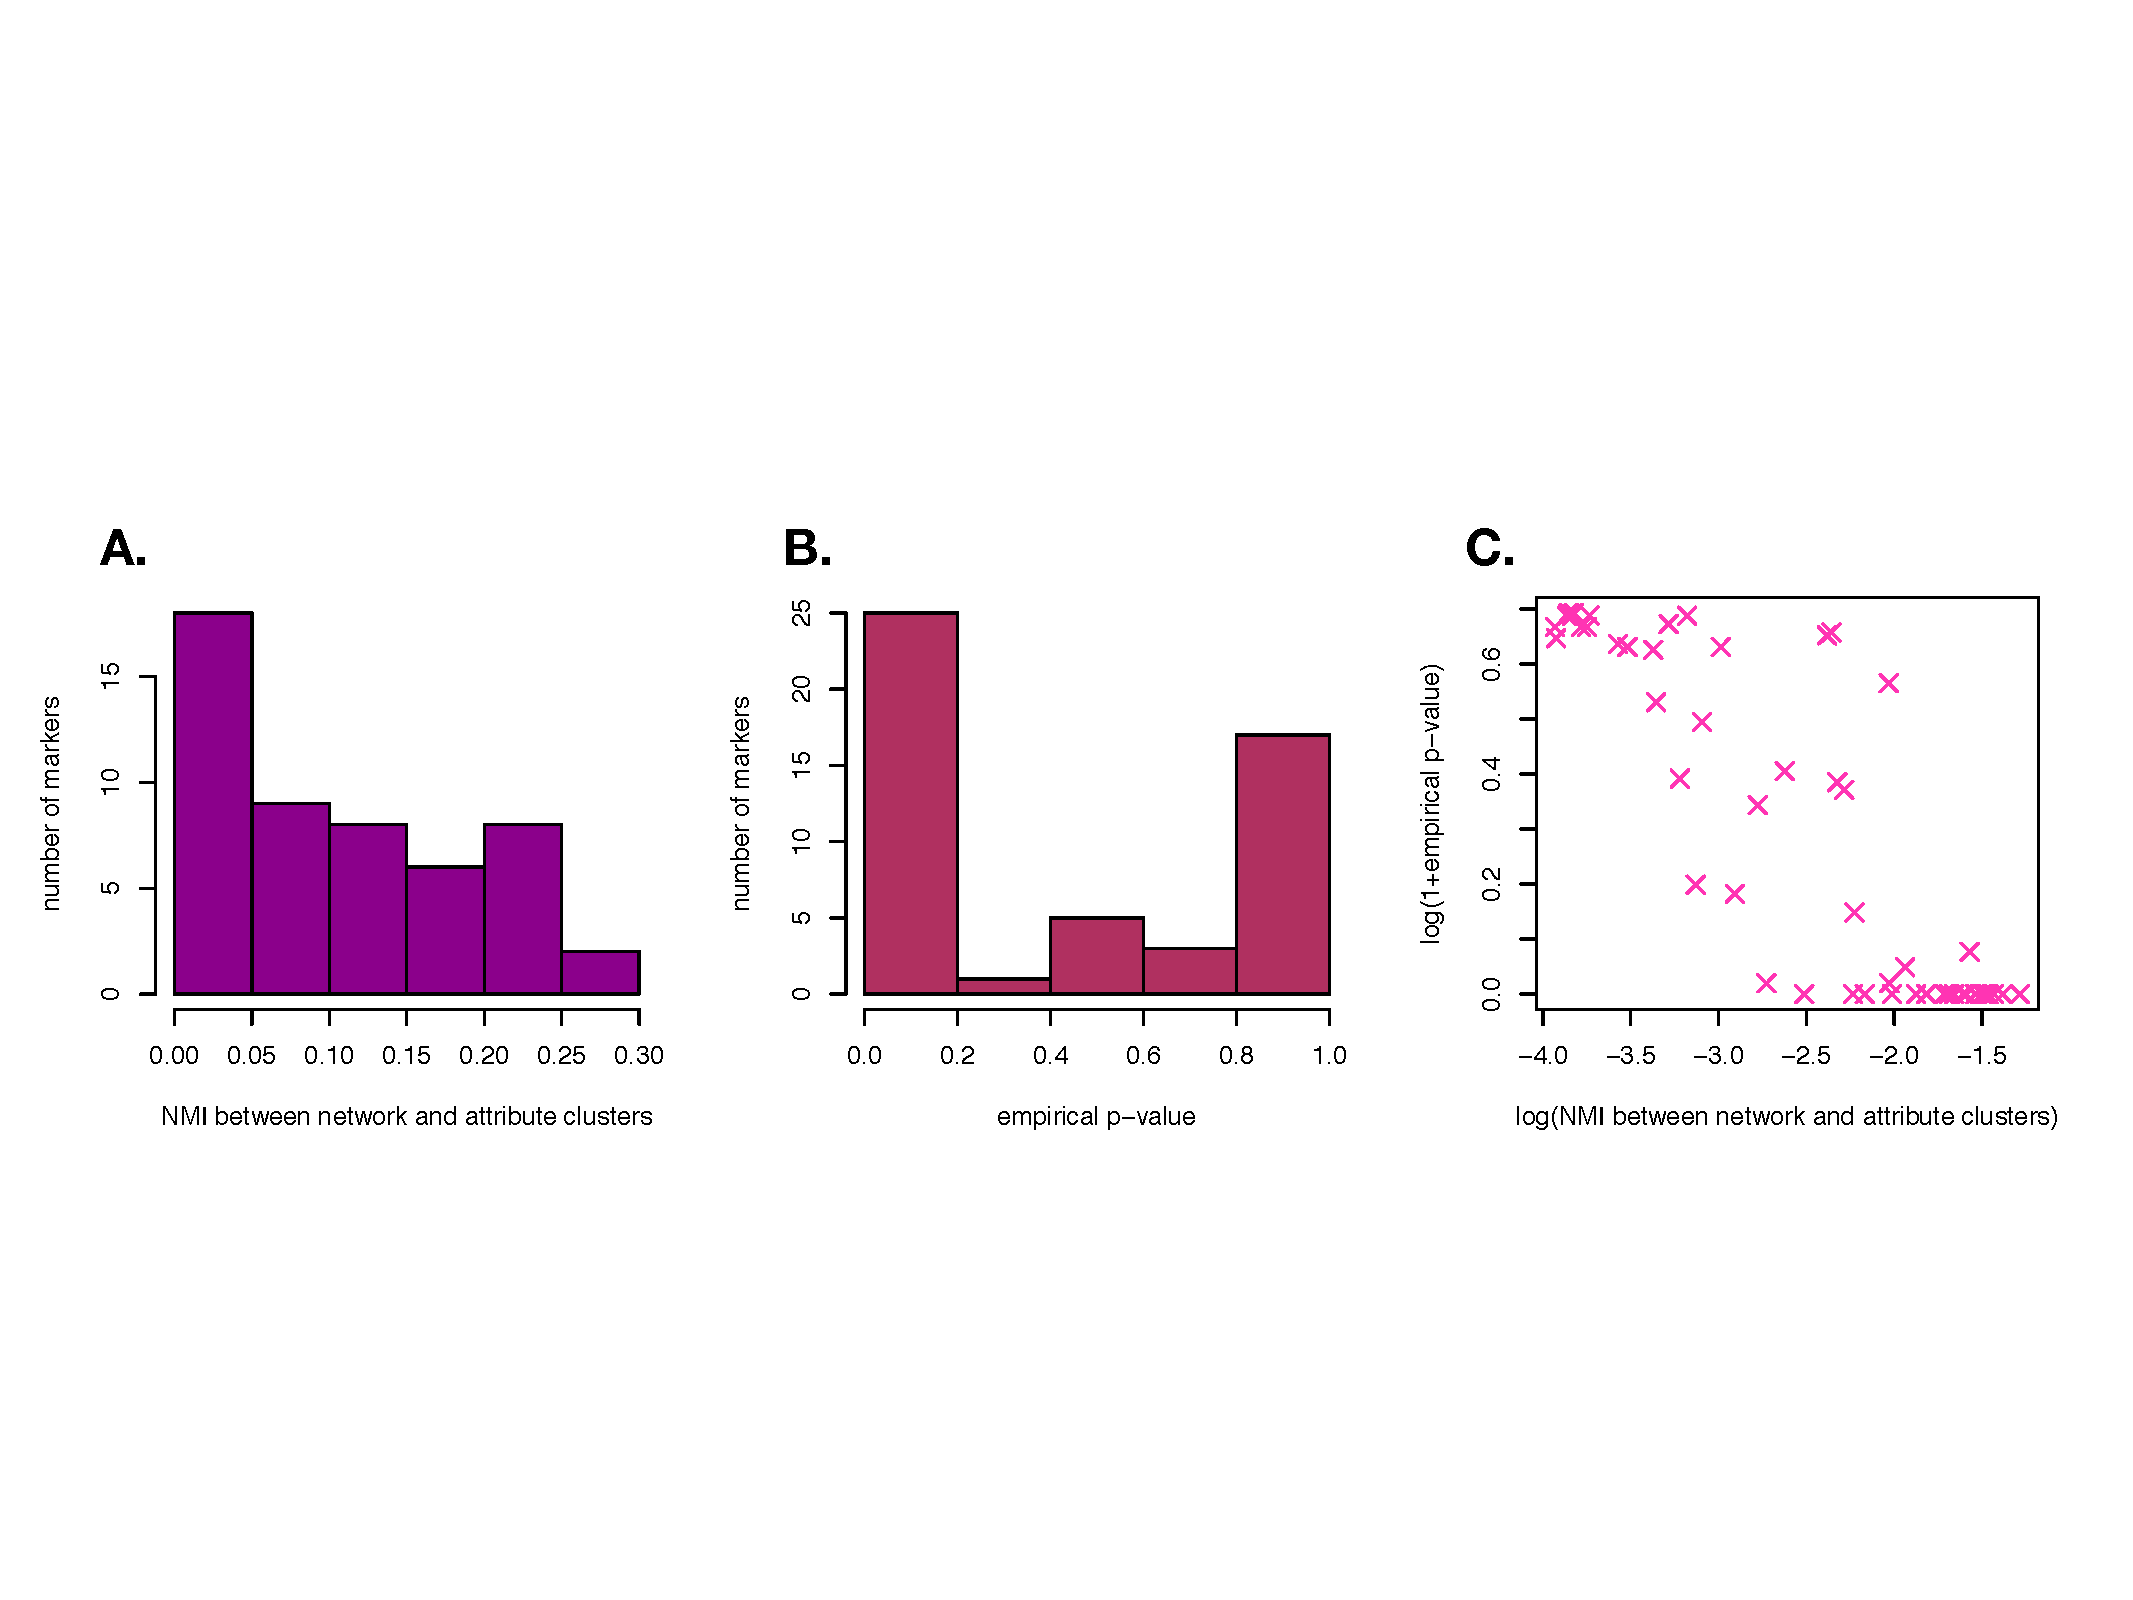
\includegraphics[width=.9\textwidth]{MakerDist.pdf}
\caption{{\bf Alignment of markers with communities.} We considered each of the possible 51 features in the single cell data and their potential to be used as markers of particular inferred cellular phenotypes. We identified 10 communities (or inferred phenotypes) under the Louvain algorithm, producing a partition of the network, ${\bf z}$. We then created a partition, $\tilde{\bf z}$ from each attribute in isolation. For each attribute and its induced partition of the nodes, $\tilde{\bf z}$, normalized mutual information (NMI) was used to measure the discriminative power of the marker in distinguishing network communities, or NMI($ \tilde{\bf z},{\bf z}$). We expected that our $p$-value should align with this NMI measure in that markers leading to high NMI between the induced $\tilde{\bf z}$ and ${\bf z}$ should have more significant $p$-values. {\bf A.} We used a histogram to visualize the distribution of NMI values across the 51 possible markers, with many of them leading to low NMI (between 0 and 0.1). {\bf B.} Similar to {\bf A.}, we visualized the empirical $p$-value for the 51 possible markers. {\bf C.} We compared the relationship between the empirical $p$-value (vertical axis) and NMI($ \tilde{\bf z},{\bf z}$) (horizontal axis) across the 51 possible markers. As expected, we observed these quantities to be anti-correlated in that more significant (lower) empirical $p$-values were obtained for higher values of NMI($ \tilde{\bf z},{\bf z}$).}
\label{MarkerDist}
\end{center}
\end{figure*}

The first test we performed on the single cell mass cytometry network was to examine how each marker feature related to the community partition, ${\bf z}$ identified with the Louvain algorithm. To assess this first without using our method, we used each of the 51 features in isolation to generate a partition of the network, $\tilde{\bf z}$. Since this generate a single continuous feature for each node, we computed $\tilde{z}$ in each case with $k$-means across the 1000 cells, with 10 clusters. We chose 10 clusters so that ${\bf}$ and $\tilde{\bf z}$ would be on the same scale. Before applying our LP test to this network, we used normalized mutual information (NMI) \cite{commdeccompare} to quantify the similarity between ${\bf z}$ and $\tilde{\bf z}$. A high NMI (i.e. close to 1), indicates that the attribute used to create $\tilde{\bf z}$ creates a similar partition to the ${\bf z}$, obtained from the Louvain algorithm. Conversely, an NMI near 0 idicates that when nodes (cells) are clustered based on the particular feature, their partition is very similar to that obtained using connectivity information. 

\begin{figure}[h!]
\begin{center}
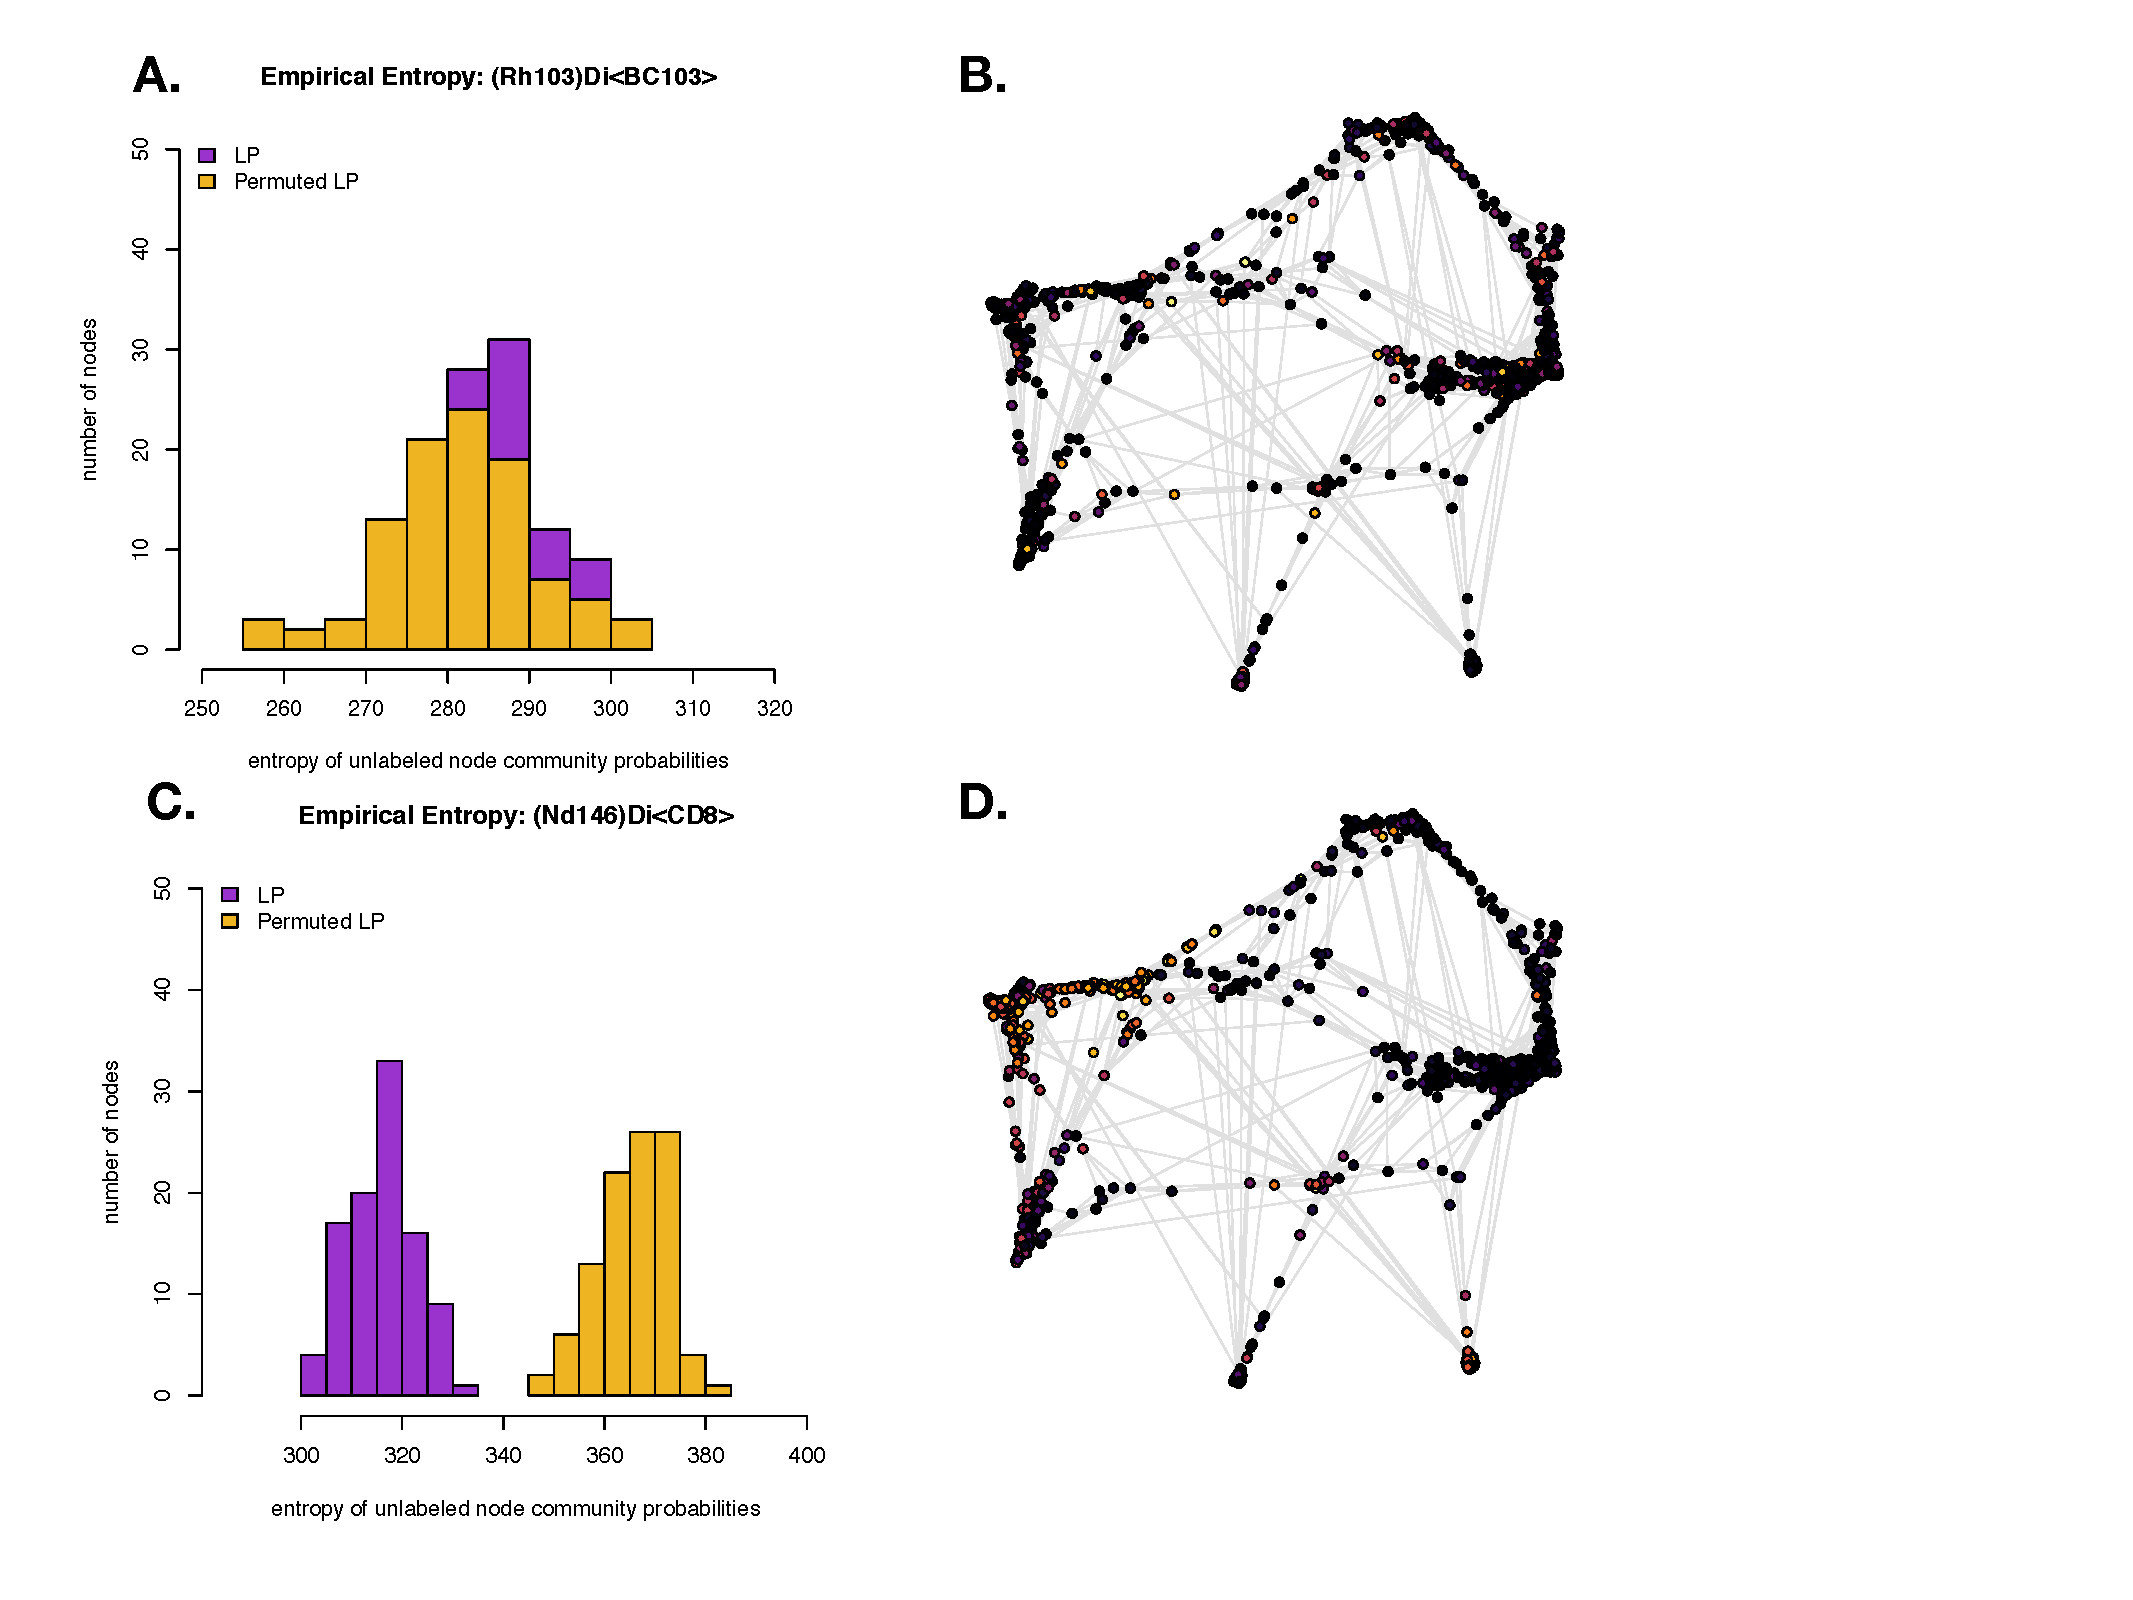
\includegraphics[width=.8\textwidth]{MassCytometry.pdf}
\caption{{\bf Validation with a well and poorly aligned markers}. We used two markers with different correlation strength with communities as another validation of the computed entropy under label propagations. First, we defined a labeling of the nodes, $\tilde{\bf z}$ based on marker (Rh103)Di$<\text{BC103}>$ that did not vary across communities in its expression, and hence not discriminate between the communities. {\bf A.} We visualized the distribution of $\mathcal{E}$ (purple), in comparison to  $\mathcal{E}_{\text{perm}}$ (gold). Since this marker has low discriminative power, we expected the shown overlap between $\mathcal{E}$ and $\mathcal{E}_{\text{perm}}$. {\bf B.} We plotted the network of the 1000 single cells and colored nodes by their expression of (Rh103)Di$<\text{BC103}>$, with lighter colors indicating higher expression. It is difficult to notice clustering in this network between cells with similar expression values. {\bf C.} Conversely to the result shown in ({\bf A.}), we chose a marker with high discriminative power, (Nd146)Di$<\text{CD}8>$. Again, we show the distribution of $\mathcal{E}$ (purple), in comparison to  $\mathcal{E}_{\text{perm}}$ (gold). Since this marker has good discriminative power, $\mathcal{E}$ and $\mathcal{E}_{\text{perm}}$ do not overlap. {\bf D.} We plotted the network of single cells, with nodes colored according to the intensity of (Nd146)Di$<\text{CD}8>$, with lighter colors indicating higher expression.}
\label{MassCy}
\end{center}
\end{figure}

In Figure \ref{MarkerDist}A. we show the distribution of NMIs computed between ${\bf z}$ and $\tilde{\bf z}$ for each of the 51 potential markers. We observe a fairly broad range or marker qualities represented. Similarly, we applied our LP task for $T=500$ trials. Figure \ref{MarkerDist}B. shows the distribution of empirical $p$-values from our LP method. We noticed that there are approximately 25 markers with a low $p$-value (between 0 and 0.2), according to our LP test. The majority of the markers do not have significant $p$-values, which is also reflected in Figure \ref{MarkerDist}A. for the markers having an NMI $<0.1$. Finally, in Figure \ref{MarkerDist}C., we examined the relationship between the NMI between ${\bf z}$ and $\tilde{\bf z}$ and the empirical $p$-value, across each of the 51 markers. As expected, these quantities are highly related, with high values of NMI corresponding to lower, more significant $p$-values.

To visualize how particular markers correlated with communities in the network, through their induced partition, $\tilde{\bf z}$,we chose a marker with low empirical $p$-value, (Nd146)Di$<\text{CD}8>$, and a marker with high empirical $p$-value, (Rh103)Di$<\text{BC103}>$. In Figure \ref{MassCy}, we sought to visualize both the entropy distributions, $\mathcal{E}$ and $\mathcal{E}_{\text{perm}}$, as well as the communities colored by the expression of each marker. In Figure \ref{MassCy} A. and C., we show the empirical entropy distributions, $\mathcal{E}$ (purple) and $\mathcal{E}_{\text{perm}}$ (gold). For the marker with significant empirical $p$-value, (Nd146)Di$<\text{CD}8>$ (Figure \ref{MassCy}C., the the empirical entropy distributions do not overlap. Conversely, for the poorly predicted marker, (Rh103)Di$<\text{BC103}>$, there is strong overlap between the empirical entropy distributions (Figure \ref{MassCy}A.). In Figure \ref{MassCy} C. and D., we colored the communities identified by Louvain by the intensities of the markers, (Rh103)Di$<\text{BC103}>$ and (Nd146)Di$<\text{CD}8>$, respectively. Light colors indicate a high marker expression, while darker colors indicate low expression. In Figure \ref{MassCy}B., where nodes are colored according to (Rh103)Di$<\text{BC103}>$, we see that nodes with high intensity expression are scattered around the network and not confided to a particular community. However, in Figure \ref{MassCy}D., where nodes are colored by (Nd146)Di$<\text{CD}8>$, many high expression markers are confined to the same community. This analysis further confirms that our empirical $p$-value is identifying markers with discriminative power because they are well-correlated with certain communities.

\begin{figure}[h!]
\begin{center}
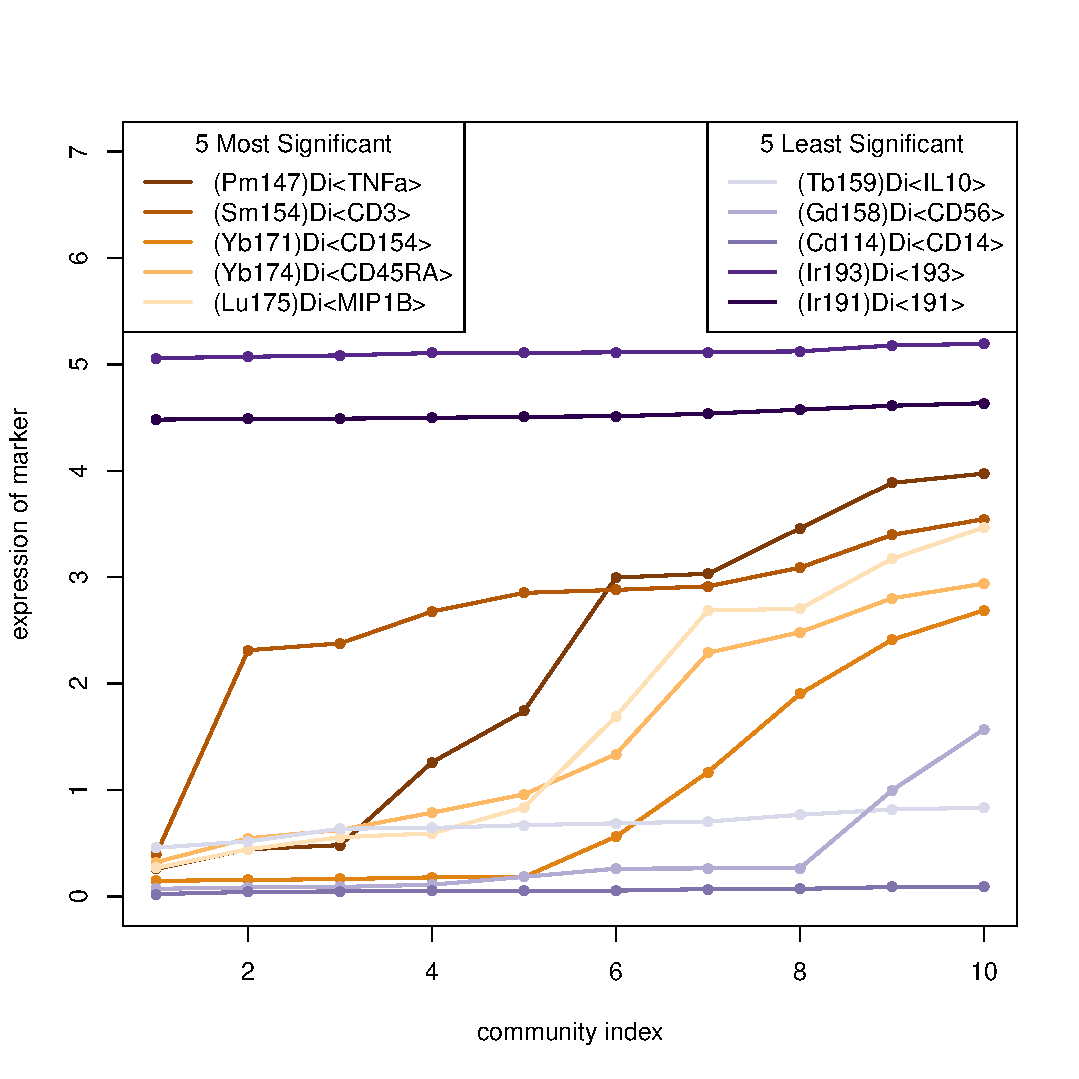
\includegraphics[width=0.8\textwidth]{MakerRank.pdf}
\caption{{\bf Variation of markers with significant empirical $p$-values across communities}. We computed the empirical $p$-values induced by the partition $\tilde{\bf z}$ for each of the 51 markers and looked closely at the top and bottom 5 markers, as inferred through the empirical $p$-value. Since a quality marker in this case is said to be one that induces a labeled of the nodes, $\tilde{\bf z}$ similar to the result obtained under the Louvain algorithm ${\bf z}$, we expect the expression of such a marker to vary across communities. In this plot, we show the expression of each marker as a function of the community index. The family of orange-colored lines correspond to the top 5 predicted markers (according to empirical $p$-value). From all of these lines, the expression varies across communities. Conversely, we plotted the lowest-ranked markers (in terms of empirical $p$-value and their expression is relatively constant across all communities.}
\label{MarkerRank}
\end{center}
\end{figure}

As an final experiment, we sought to see if the markers with significant empirical $p$-values (implying that they are effective in distinguishing cellular phenotypes) did indeed vary across communities in the network, through their induced partition, $\tilde{\bf z}$. To do this, we selected 10 markers from the 51 measured features of the single-cell data. In particular, we looked at the 5 most and least significant markers, in terms of the computed empirical $p$-value. For each of these 10 markers, we computed the mean marker expression across each of the 10 communities, identified by applying the Louvain algorithm \cite{blondel} algorithm to ${\bf A}$. We then plotted the mean marker expression across communities for the 5 most and least significant markers in Figure \ref{MarkerRank}. The least significant markers are shown in the family of blue lines and are relatively static across each of the 10 communities. In contrast, the orange family of lines corresponds to the markers for the top 5 most significant communities and do vary across communities. Since a marker with a significant low empirical $p$-value should correlate well with communities, this is the pattern we expected. The 5 poorly ranked markers clearly do not correlate with communities because their expression is constant across all communities.

\section{Conclusion}
In this paper, we introduced a label propagation based approach to determine how closely attributes align with network connectivity. To label propagation task seeks to predict the labels for an unlabeled set of nodes, according to the initial partition of the nodes according to the attribute information, $\tilde{\bf z}$. The label propagation task we adopt returns a probability distribution for each of the unlabeled nodes over the possible communities. The empirical $p$-value of our test is computed by comparing the empirical entropy distributions from our label propagation task, and a permuted label propagation task, denoted by $\mathcal{E}$ and $\mathcal{E}_{\text{perm}}$, respectively. The intuition is that if attributes are well aligned with network connectivity patterns, then the label propagation task should produce results that are more certain, and hence have lower entropy. Our results indicate that the computed entropy and empirical $p$-value are behaving as expected on synthetic example, where we designed the experiments in a way that we knew how well the attributes and connectivity correlated. We also show that our test is useful in the identification of important marker features for distinguishing communities in the single cell mass cytometry network. Here, features (markers) with low empirical $p$-value as features that vary across communities and hence give insight into what distinguishes the communities. 

As future work, we can examine how the entropy and empirical $p$-value relate the the quality of communities identified across the variety of community detection approaches. For example, perhaps our test is more aligned with the assumptions of the stochastic block model than label propagation. Finally, similar to how we detected particular marker features that were aligned with the identified communities, perhaps we can use our tool as a feature selection method that can enable a meaningful network representation of the data. 


\chapter{A network approach to understanding microbiome disruption in response to acute lung injury}
\indent As the final chapter in this thesis, we present an application of how network analysis and community detection were used to understand the changes in the microbiome composition of patients acute lung injury. Analogous to the discussions related to microbiome analysis earlier in this thesis, the profiling of the microbiome is accomplished through metagenomic sequencing and identifying OTUs (operational taxonomic units). Each OTU is treated as a taxonomic unit, or bacterial species and typical microbiome analyses look at the counts of a collection of OTUs across samples. In this work, we seek to study how the co-occurence patterns of OTUs differ between healthy patients and those with acute lung injury. We show that creating a network representation of this data and analyzing it with community detection is crucial for the ability to understand functional differences between two cohorts of patients.

\section{Background and Motivation}
 This study is a follow-up analysis to the work by Walsh \emph{et al.}, which sought to profile the microbial composition of patients with acute lung injury (ALI) from smoke \cite{walsh2017}. This analysis shows that patients with acute lung injury have enrichment for different taxa than healthy patients, however the co-occurence patterns between pairs of species was not investigated. it is interesting to study these co-occurence patterns because specific types of pairwise interactions between species lead to different functions of the involved individuals \cite{boon}.  In these interactions, bacteria undergo processed, such as, exchanging intermediate compounds to make amino acids or lateral gene transfer. Pairwise interactions can be classified as being mutualistic, where all species in an interaction benefit , or antagonistic, where some species benefit at the expense of others \cite{mutualism}. The identification of important pairwise interactions between taxa offer the opportunity for therapeutic intervention.  
 
 \subsection{Data Background}
\indent DNA was extracted from bronchial washings of 48 patients after 72 hours of hospitalization for burn and inhalation injury in the North Carolina Jaycee Burn Center. Patients were classified as having burn inhalation injury as hypoxemia according to the ration of the partial pressure of arterial oxygen ($PaO_{2}$) (P) to the fraction of inspired oxygen ($FiO_{2}$) (F) $\le 300$. A. patient with a P/F ratio $>300$ was assumed to have normal oxygenation levels. Those with P/F $<300$ were classified as having acute lung injury (ALI). DNA was sequenced using the MiSeq \cite{miSeq} platform and bacterial species were identified using the MT-Toolbox pipeline \cite{your}. The output of MT-Toolbox was an OTU count table, profiling the abundances or counts of 372 OTUs for each of the 48 patients.

\section{Network Analysis Methods}
\subsection{Creating Networks with SparCC}
\indent Given the OTU count table that we generated, the next objective was to construct 2 networks. The first network being the OTU co-occurence network, constructed from the 24 patients with acute lung injury. The other network is the OTU co-occurence network between healthy patients. To construct these networks, we used SparCC \cite{sparcc}, the method discussed in chapter 2. As a recap, the objective of this method is to create sparse correlation networks between OTUs, based on their counts. Pearson correlation can be used to compute these correlations, bit suffers from the count-based nature of the data, producing spurious correlations. The authors further point out that spurious correlations are often worse when the diversity of the sample (defined as some function of the number of OTUs present) is low. Hence, SparCC is a state-of-the-art method because it takes this issue into account. The correlation network in each case  is between OTUs, according to their co-occurence patterns across patients in the associated cohort (healthy vs. acute lung injury). \\
\indent The correlation networks returned by SparCC had both positive and negative edge weights. In this analysis, we only consider positive edges, as most of the the community detection literature is not amenable to signed networks. We were further curious to see how we could more closely hone in on the important structures by thresholding the network, or removing edges less than some threshold weight. We based this threshold on two criteria. First, we sought to find a stable threshold where slight variations in thereshold would not dramatically change the number of communities detected with a modularity-based community detection algorithm. Next, we also sought to identify the threshold producing a node-to- community partition similar to the results produced at an adjacent threshold. In summary, both of this methods seek to find a stable threshold that does not dramatically change the community structure. For both networks, this threshold turned out to be 0.14. In other words, we discarded edges with a weight less than 0.14. This produced 4 communities (identified through modularity optimization) in each network. We show the acute lung injury and healthy OTU co-occurence networks  (left and right, respectively) in Figure \ref{alinet}. Here, nodes are colored by their community assignment. From even this early glance, we observe that the structures of these networks are quite different. This observation allowed us to further analyze the difference in biological function reflected in these different network structures.  


\begin{figure}[h!]
\begin{center}
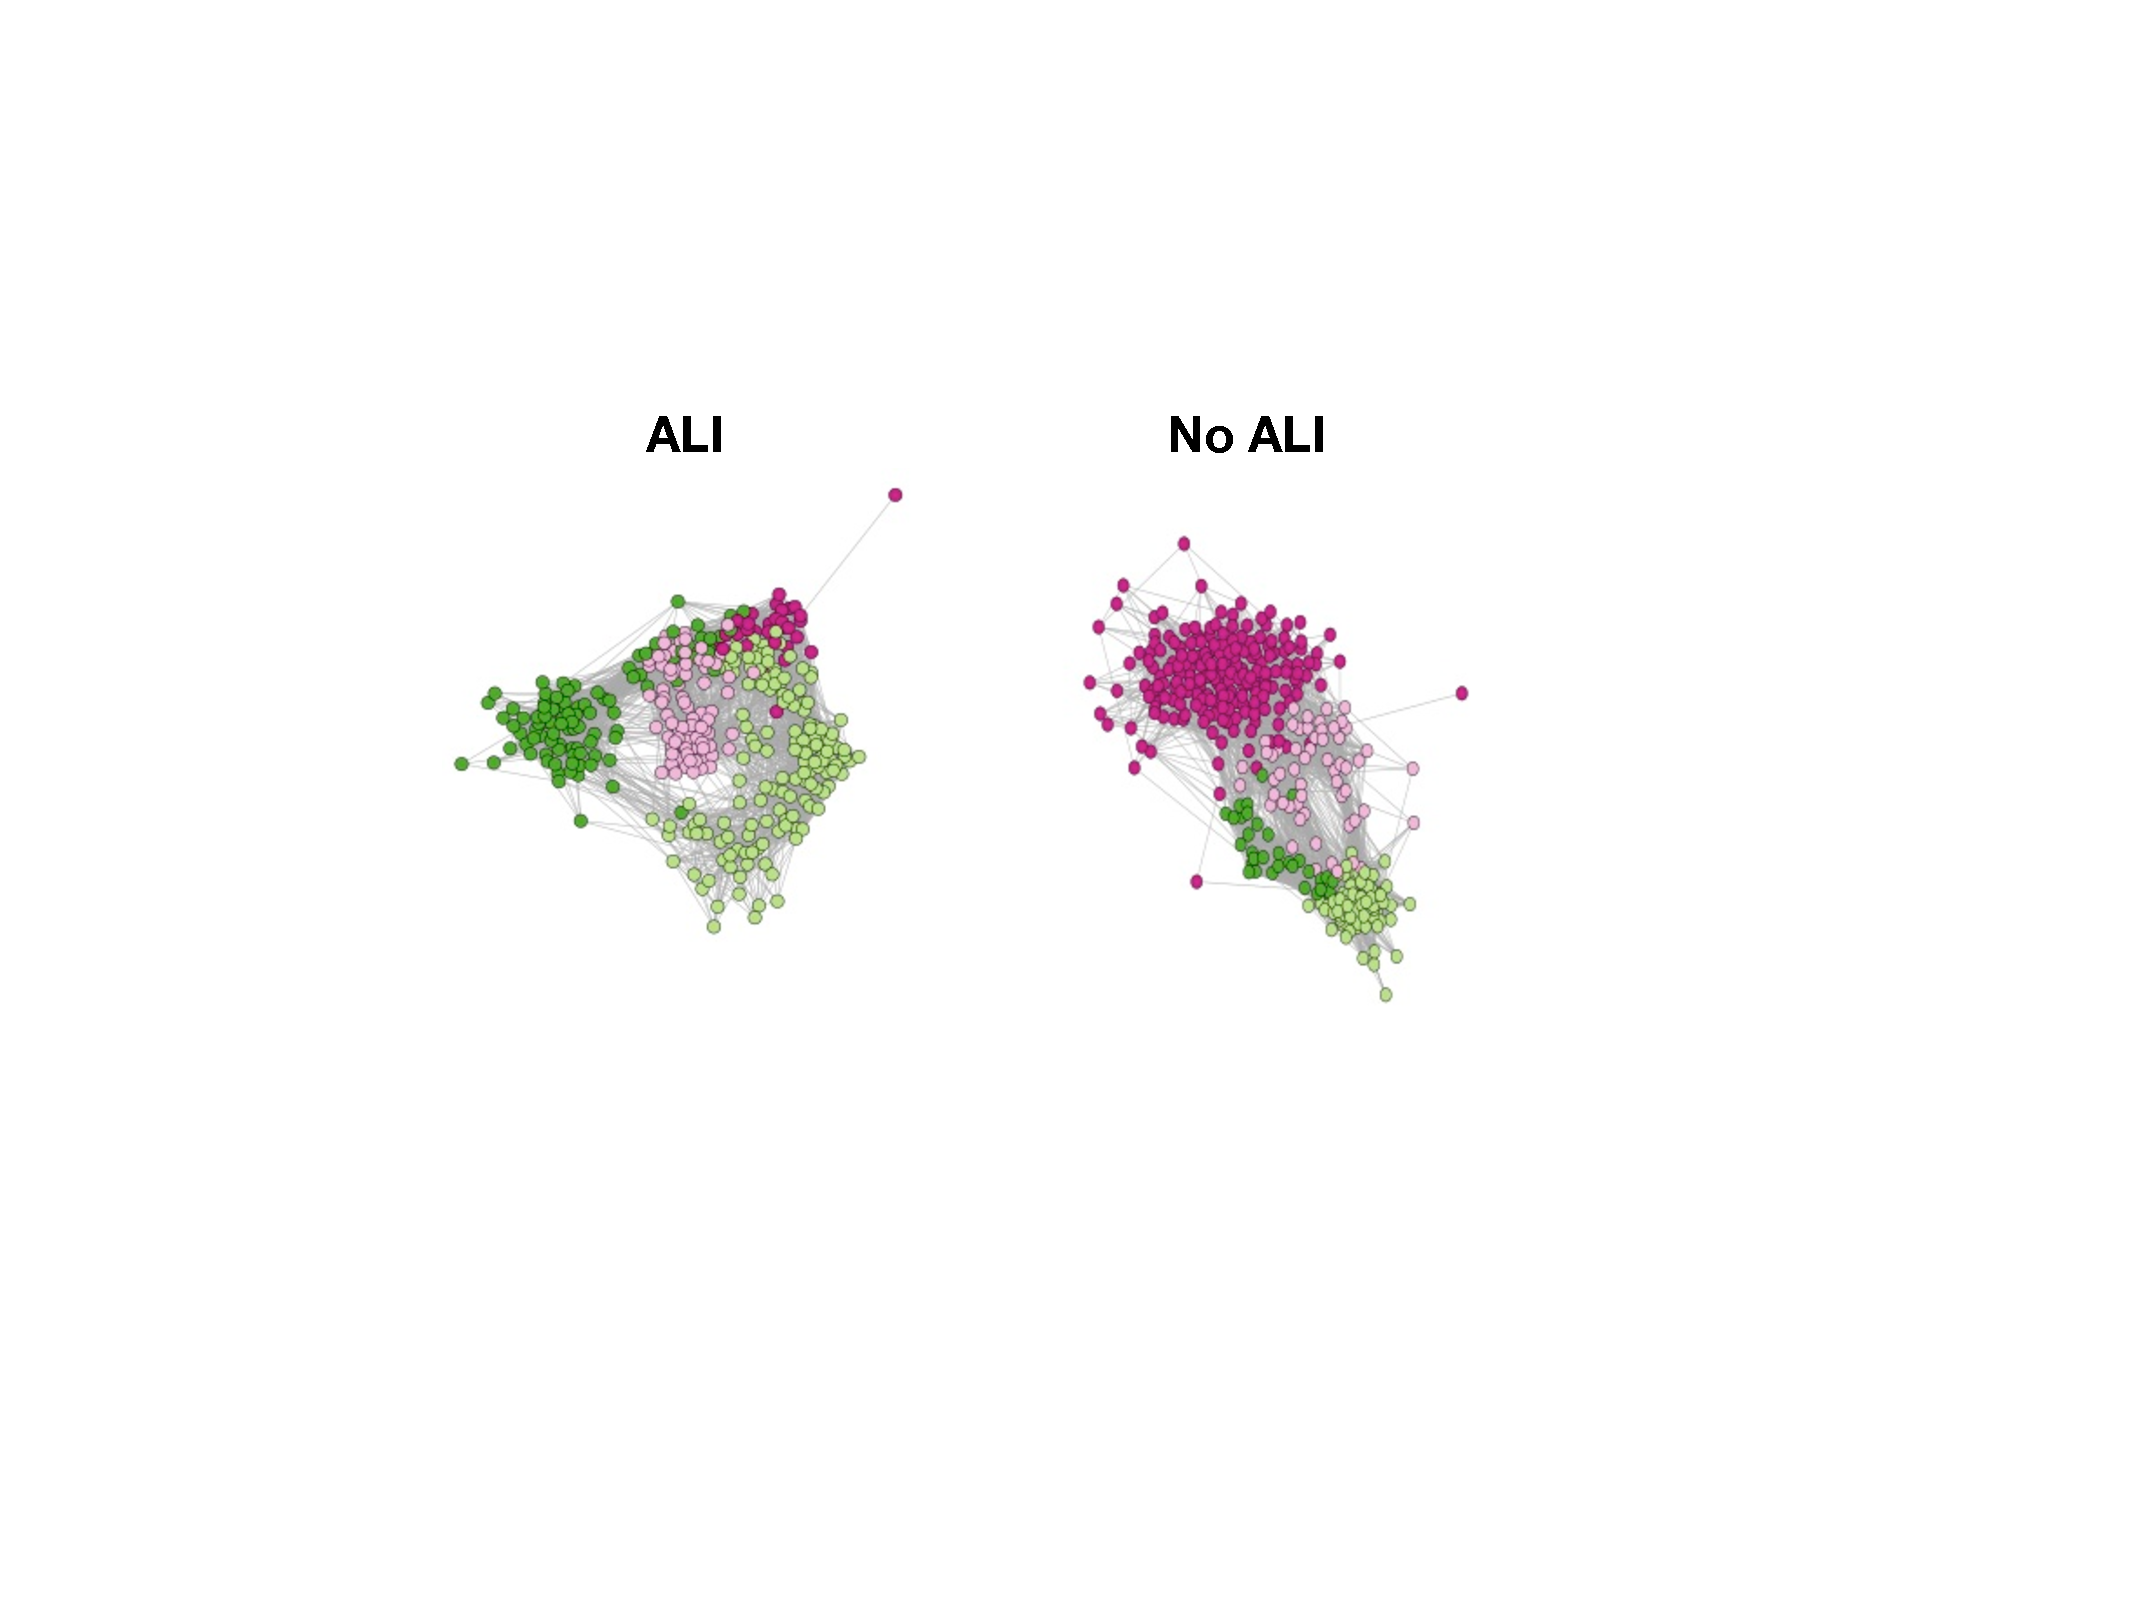
\includegraphics[width=0.7\textwidth]{ALINet}
\caption{{\bf Microbial co-occurence networks for each patient cohort}. We constructed networks with SparCC in the ALI and non-ALI cohort networks (left and right, respectively). Four communities were identified in each network. Nodes are colored by their community assignment.}
\label{alinet}
\end{center}
\end{figure}

\section{Results}
\subsection{Community overlap between network}
\indent After constructing the network for each cohort, we first evaluated the similarity in all pairs of communities across both networks, and used bioinformatics tools to further uncover the biological differences. We denote the communities in the ALI network by ALI 1, ALI 2, ALI 3, and ALI 4. Similarly, we denote the four communities in the No ALI network by No ALI 1, No ALI 2, No ALI 3, and No ALI 4. In table \ref{Tab5}, we show the contingency tables, where each entry counts the number of OTUs shared between the community pair. We denoted the large overlaps (i.e. sharing many common OTUs) by pink shading in the table. In particular, we highlight the similarity between ALI 4 and No ALI A, ALI 3 and No ALI B, ALI 1 and No ALI C, and ALI 2 and No ALI D. 

\begin{table}[]
\centering
\label{my-label}
\begin{tabular}{lllll}
      & No ALI A                                          & No ALI B                   & No ALI C                   & No ALI D                                          \\
ALI 1 & 1                                                 & 1                          & \cellcolor[HTML]{EEB6D1}27 & 2                                                 \\
ALI 2 & \cellcolor[HTML]{FFFFFF}50                        & 5                          & 9                          & \cellcolor[HTML]{EEB6D1}{\color[HTML]{333333} 22} \\
ALI 3 & 66                                                & \cellcolor[HTML]{EEB6D1}46 & 37                         & 5                                                 \\
ALI 4 & \cellcolor[HTML]{EEB6D1}{\color[HTML]{333333} 77} & 5                          & 15                         & 4                                                
\end{tabular}
\caption{{\bf Comparing Networks in Each Patient Cohort}. We compare the OTUs in each pair of communities in the ALI and No ALI cohort networks. Large overlaps are denoted by pink shading in the table.}
\label{Tab5}
\end{table}

\subsection{Evaluating functional differences}
\indent Next, we sought to study functional differences in the airway microbiota between patients with and without acute lung injury. In other words, each of the OTUs contains different genes, which leads to different functions (i.e. containing many genes that encode glycoside hydrolase activity). Moreover, we hypothesized that there would be a difference in the functions of the communities between the ALI and non ALI networks. To investigate this, we used PICRUSt \cite{picrust}, a bioinformatic approach used to predict the function of each community. PICRUSt works by looking at each community and the known genetic information about the OTUs assigned to that community and determining the enrichment of particular functions. 

\subsection{Classifying each community according to predicted function}
\indent PICRUSt originally returned 6,911 unique functions according to the communities across both networks. We were interested to see if we could train a classifier to predict an OTUs community assignment based on its inferred function, according to PICRUSt. In other words, each OTU has several predicted functions, according to its genetic content and we wished to test if we could predict an OTUs community assignment in each network based on the presence or absence of certain functions. From the 6,911 features returned by PICRUSt, we reduced the set by filtering out the functions that were not associated with any OTU. We further filtered out functions if they had a small ratio of within-class variance to between-class variance, meaning that we only wanted features that varied a lot between classes. Using a ratio threshold of 0.05 brought the number of features in our model to 328. A random forest model was trained with half of the data for the ALI and No ALI datasets independently.  To visualize which features were most predictive in being able to classify an OTU into a community, based on function, we measured its importance their importance based on their Gini importance \cite{gini}. In Figure \ref{Function}, the biological functions are presented from top to bottom for the ALI and No ALI networks (left and right, respectively) in terms of their Gini score.

\begin{figure}[h!]
\begin{center}
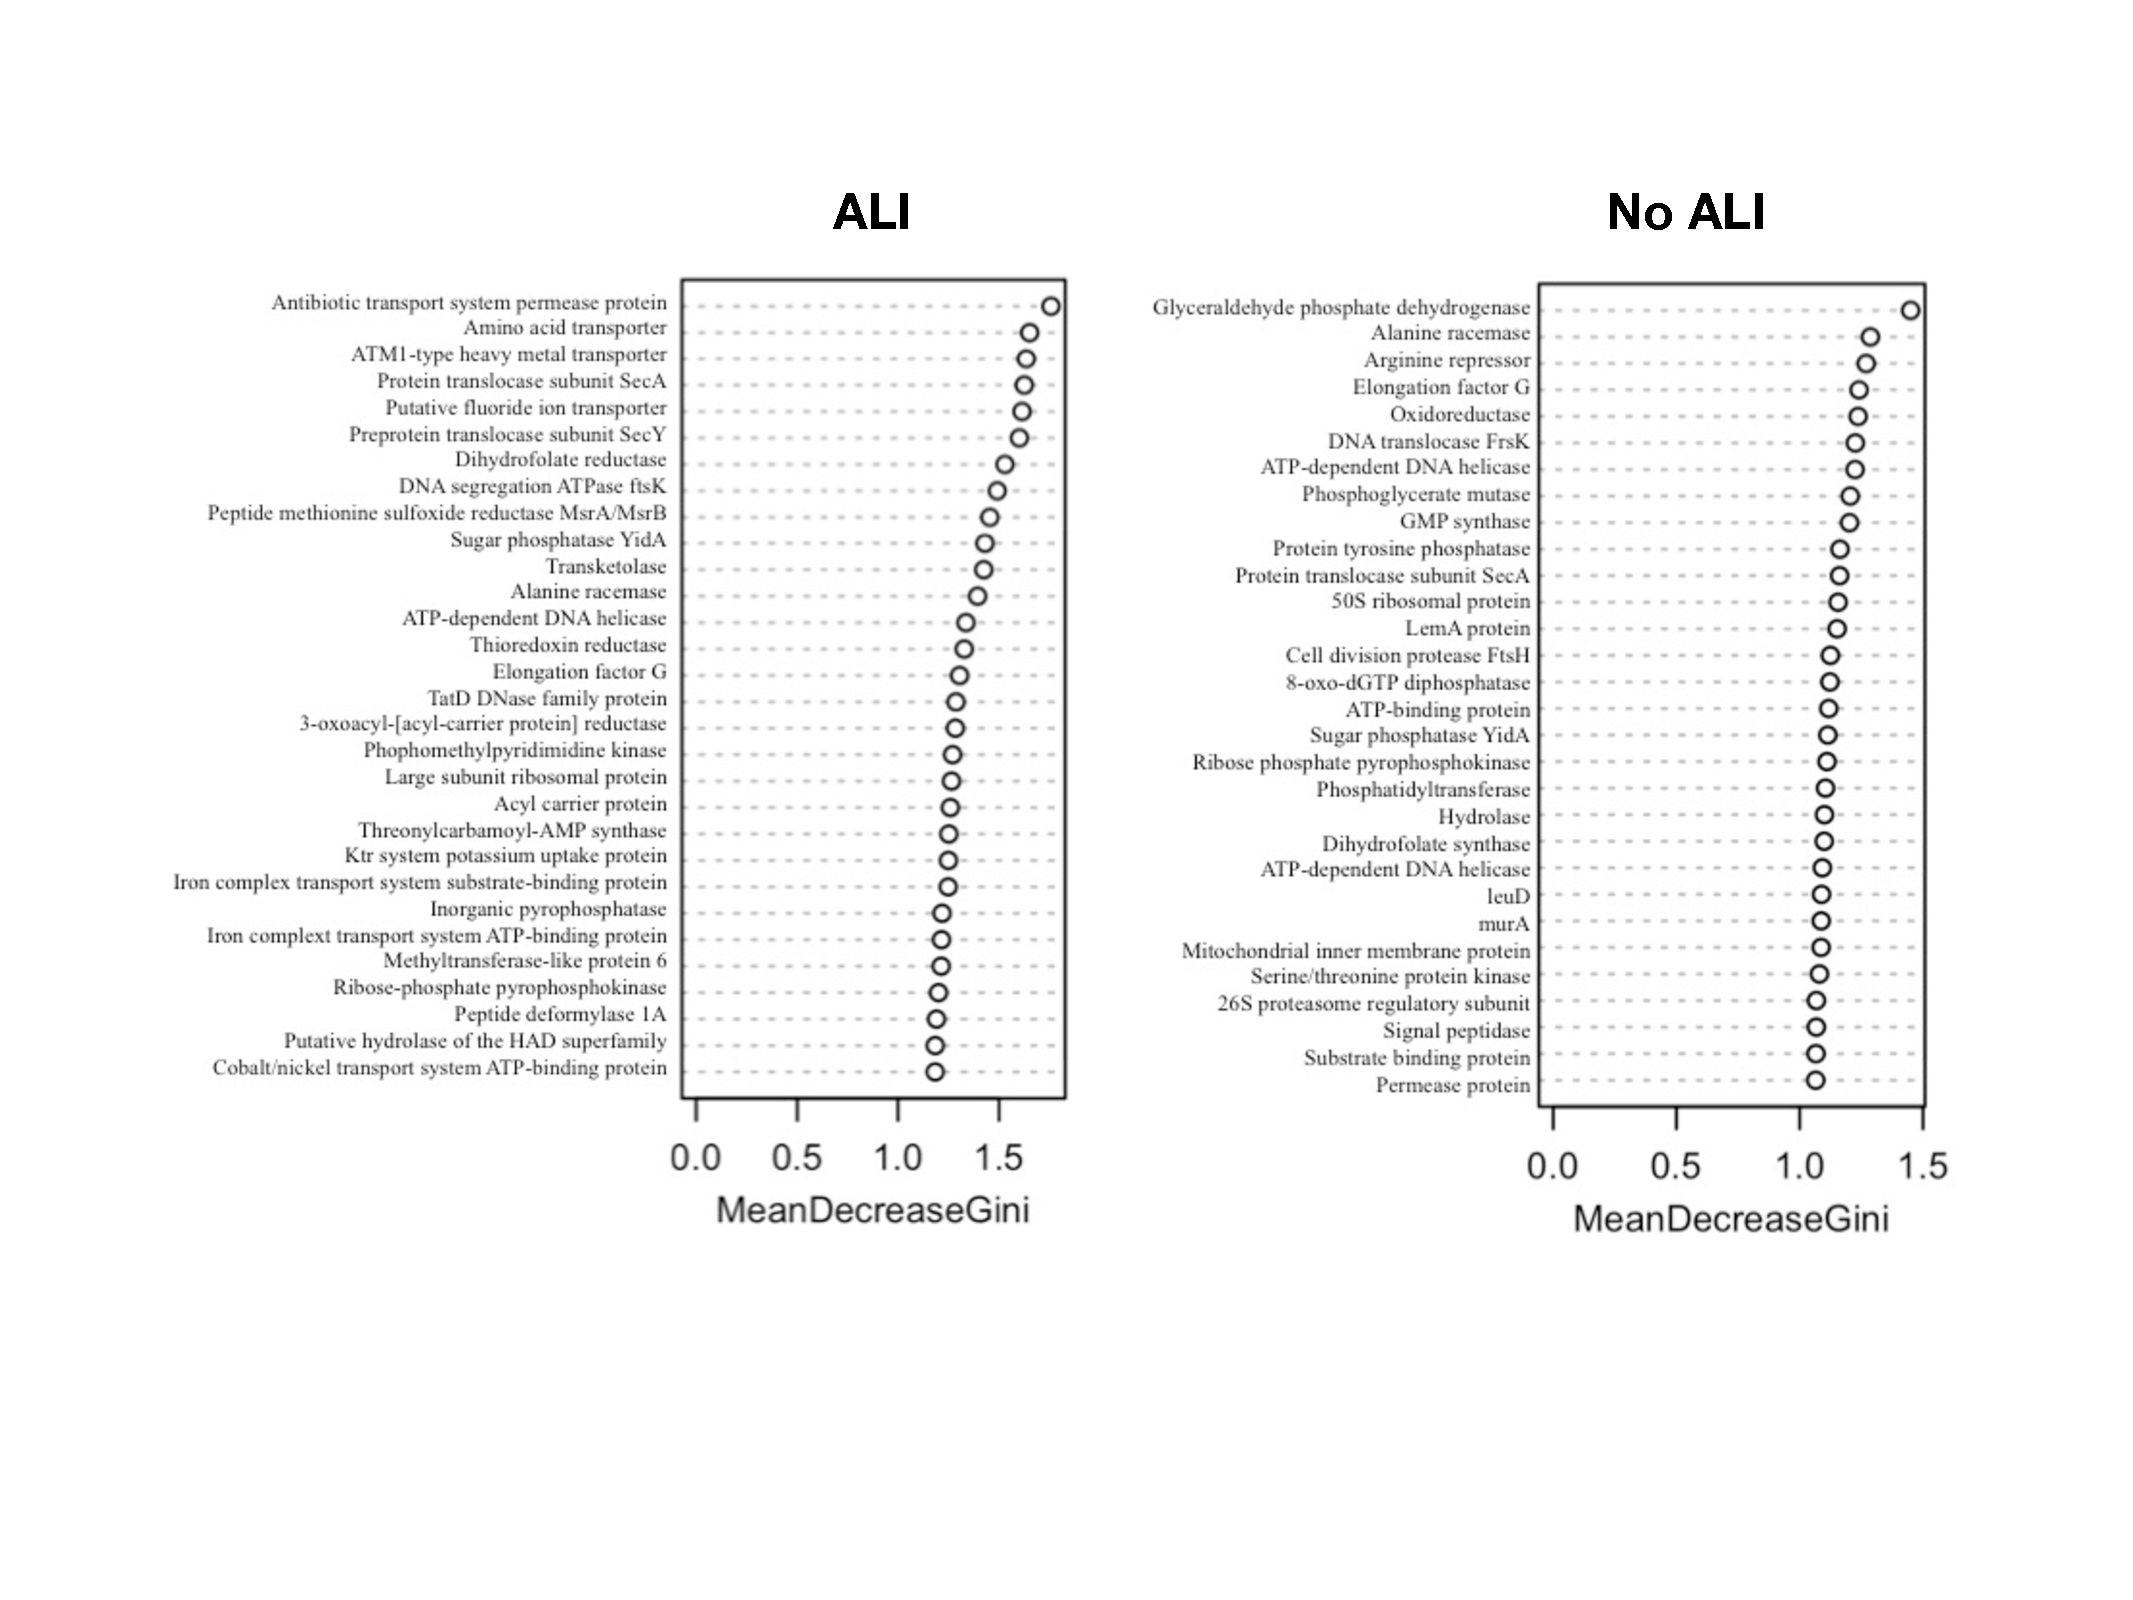
\includegraphics[width=0.9\textwidth]{Function}
\caption{{\bf Predictive functions for community classification}. We used a set of 328 filtered functions to predict OTU-to-community assignment in the ALI and No ALI network (left and right, respectively). Biological features with more discriminative ability in classification from the random forest classifier are ranked higher on the list.}
\label{Function}
\end{center}
\end{figure}

When these highly ranked predictors were compared between the ALI and no ALI networks, there was very little observed overlap between the highly ranked features between the ALI and no ALI networks, which suggested that acute lung injury is severely altering the microbiome and its function.

\section{Discussion}
\indent In this chapter we presented preliminary work with an approach to better understand the disruption and evolution to the microbiome in response to acute lung injury. Recognizing the importance of not just measuring the abundances of OTUs in a sample, but also the species that it occurs with offers more in-depth insight into the underlying biological processes occurring. Constructing networks with SparCC for each of the ALI and No ALI cohorts allows us to probe the structural organization of these two different networks. The PICRUSt bionformatics tool and classification task provided important insight into the biological functions that are most indicative of each community in the ALI and No ALI networks. As shown in Figure \ref{Function}, the antibiotic transport system permease protein was ranked to be the most predictive in terms of classifying the OTUs into communities. This might suggest that patients with ALI are better able to transport antibiotics out of the cell, making them more resistant to treatment. This observation suggests that future work should be done to determine if \emph{Prevotella melaninogenica}, an enriched species shown by Walsh \emph{et al.} contains the antibiotic transport system permease protein and gives bacteria an advantage in resisting antibiotic treatment and remaining  in the airways of patients with ALI. \\
\indent Overall, this work prioritized microbial interactions and potential biological mechanisms (specifically antibiotic resistance) that can be further investigated in the lab to understand the implications of acute lung injury on the microbial ecosystem in airways. 

\chapter{Conclusion and Future Work}
In this thesis, we presented three new methods that enable network analysis on more diverse types of networks. In this section, we will recap each of the developed methods, explain possible extensions to the work, and describe classes of problems or applications that may benefit from such an approach.

\section{sMLSBM}
\subsection{Recap}
We first presented the strata multilayer stochastic block model (sMLSBM), an extension to the standard stochastic block model that fits a collection of models to a multilayer network. Seminal approaches to fit an SBM to a multilayer network used all of the layers together to learn a single stochastic block model to describe a multilayer network. Moreover, our approach is novel because it assumes that there are potentially multiple stochastic block models that have given rise to the collection of networks. By learning a set of stochastic block models, each model corresponding to a `stratum', we have the ability to cluster networks and to understand the generative process that gave rise to each layer. We have shown this is useful in the microbiome example, shown in Figure \ref{sampleNet}, where we visualized the SparCC-generated correlation networks  across body sites. From this figure, it is clear that sets of networks have very different structures and fitting the same model to all of the layers together would not provide a meaningful summary of the data. We can summarize the implications of this work as follows.First, we show that the SBM fit with the collective information from all networks in a stratum can be sampled to understand a representative connectivity pattern for members of that cluster. This work inspired the investigation of detectability and how to most effectively combine the network layers within a stratum to accurately define community structure.


\subsection{Future Work}
The first two major limitations of sMLSBM is that it exists for handling unweighted networks and that fitting the model requires for the specification for the number of strata, $S$. In reality, most networks are weighted, and weights are an important aspect of structural organization. As we have alluded to, the literature for dealing with weighted stochastic block models is still in its primitive phase, as it is not immediately clear how to handle the distribution of edge weights. With increasing advances in weighted stochastic block models, this ability to extend sMSLBM to weighted networks could be valuable.\\
\indent Second, in all of the examples in this paper, we always had a rough idea about how many strata, $S$ to use. In reality, if you are looking to cluster your networks and figure out how many stochastic block models describe your multilayer network, you might not know what $S$ to choose. To temporarily mediate this issue there are a couple of hacks that can be used. First, an SBM can be fit to each network layer individually and the corresponding adjacency probability matrices can be clustered with $k$-means, where the number of clusters can be specified with one of the many model selection criteria. Second, the adjacency probability matrices can be visualized using tSNE or PCA to guess how many clusters of networks exist in the data. Finally, since fitting sMLSBM is done in a way that maximizes likelihood, one could always compute fit multiple models with different $S$ and compare the likelihoods of the fitted models. \\
\indent One interesting application of multilayer networks in in the analysis of temporal network data, where each network layer corresponds to a point in time. It would be interesting to incorporate this time element in determining each stratum. That is, one can assume that network layers that are closer together in terms of their time step should be more likely to be members of the same stratum. If this were the case and strata were composed only of network layers that appeared sequentially in time. The breaks between these temporally-contiguous sets of networks is known as change point detection and has been previously explored for probabilistic hierarchical networks by Peel \emph{et al.,} \cite{peelChange}. \\
\indent Finally, super nodes currently operates on an assumption that each network layer belongs to a specific cluster. Given the great success in mixture models, perhaps it could be useful to model each network's membership to a cluster with a probability distribution, rather than a binary classification. 

\section{Super Nodes}
\subsection{Recap}
Next, we introduced super nodes, which is a pre-processing step for large networks before applying community detection. We discusses that the benefits of a super node representation of the network is a decreased run time of community detection algorithms, decreased variability among outputs of the community detection methods, and more consistent labeling within a local region of the network (i.e. less label entropy within a neighborhood). We demonstrated our approach on several large social network datasets. Finally, we discussed the important issue in the development of community detection approaches that results are difficult to validate without ground truth. We did our best to validate our approach with normalized mutual information and under segmentation error to compare to the results that would have been obtained by using the full network. \\
\indent Some limitations of this work is that it is for unweighted networks and we don't have evidence that the seeds chosen are the absolute best super node centers. To mediate both of these issues, it might be useful to use Random walks to choose seeds and grow out super nodes. In choosing seeds, for example, a number of random walks can be started from a large number of randomly selected nodes. The seeds of our super nodes could be the set of nodes that many random walks pass through. Furthermore, the growing out process for the super nodes could assign the non-seed nodes to the seed contained in the majority of their random walks. Random walks are a powerful tool to compress networks due to their relationship with the Graph Laplacian matrix. 
\subsection{Future Work}
\indent Since we have introduced a method to handle attributed network data, it may also be interesting to determine how attributes can be incorporated in defining a super node. This is briefly considered in references \cite{SuperNodeSide,supergenomic}, which require some notion of node attributes. However, perhaps we can incorporate node information in our growing out step.\\
\indent Given that one appeal of the super node representation of the network is that it reduces the large network to a much smaller size, it would be useful to figure out how to exploit this information for visualization, network summarization, and prediction tasks. More work should be done to determine how the summary statistics of the original network are carried over to the super node representation. For prediction tasks such as link prediction, or collaborative filtering, it would be interesting to probe how information within and between super nodes can be used to maximize predictive accuracy. 

\section{Attributed SBMs}
\subsection{Recap}
Finally, we presented an extension of the stochastic block model to handle networks, where the nodes have multiple continuous attributes. This work extends the current literature of attributed stochastic block models because it allows for multiple continuous attributes. This work also builds on the assumption that a node's connectivity and attribute data should depend on its community membership. To validate our model and inference approach, we show that the learned model can be used and obtain good performance on two prediction tasks: link prediction, and collaborative filtering. Finally, we demonstrate this performance of the attributed SBM on two biological data sets, specifically for microbiome data and protein interaction networks. 
\subsection{Future Work}
Similar to the limitations of sMLSBM and super nodes, this method is also only applicable to unweighted network and it is required to specify the number of communities expected to find. While the combination of attributes and connectivity in a weighted network is likely a challenging task, it is useful to develop a model selection criteria to decide how many communities to find. Next, the examples we have shown have included only a few continuous attributes, but it might become difficult to estimate the covariance matrix if there are many continuous attributes. The limitations of this should explored and it should also be investigated how lower dimensional representations of the attributes affect the quality of the link prediction and collaborative filtering results. Finally, we make a strong assumption in our model that connectivity and attributes are conditionally independent, given the class labels. Perhaps we can do more work in the future to determine how realistic this assumption is for a dataset of interest. \\
\indent We also briefly alluded to the detectability limits of stochastic block models and how adding attributes that are principled (or aligned with the node-to-community assignments) can affect the ability to find communities. This question can be explored more rigorously and formally. \\
\indent Finally, in the introduction, we introduced the affiliation model as a flexible probabilistic approach to model connections between nodes according to their community affiliations. Perhaps adapting the affiliation model to handle multiple continuous attributes could provide a more flexible notion of an attributed community. Given that the BIGCLAM method that we presented is achieved by optimizing a likelihood through block coordinate gradient ascent, it could be possible to simply augment the likelihood with the Gaussian attribute term. \\


% Bibliography
\clearpage
\phantomsection

{\def\chapter*#1{} % suppress bibliograph header.
\begin{singlespace}
\addcontentsline{toc}{chapter}{BIBLIOGRAPHY}
\begin{center}
\Large \textbf{BIBLIOGRAPHY}
\vspace{17pt}
\end{center}

\bibliographystyle{apalike}
\bibliography{dissBib}
\end{singlespace}
}





\end{document}
